%!TEX root = ../main.tex
% Chapter 1

%\chapter{background}
\chapter{Introduction and Problem Statement}
The purpose of this assignment is to design, simulate and implement a PI controller to compensate a DC motor using a microcontroller. The implementation will be assessed by means of a report in accordance with ECSA ELO 2, as part as the following milestones:
\begin{description}
	\item[Milestone 1] Characterisation of a DC motor
	\item[Milestone 2] Mathematical modelling and simulation of the DC motor
	\item[Milestone 3]Controller design and simulation of closed loop system
	\item[Milestone 4] Practical demonstration of controller design
	\item[Milestone 5]  Final report
\end{description}
The first milestone was completed successfully earlier in the semester and the lab report is included in appendix A. 







\chapter{Literature Study}
\section{Modeling the DC Motor}
According to the Prescribed textbook\cite[p.160]{dorf2011modern}: \\ \blockquote{\emph{Time constant}\\ The time interval necessary for a system to
change from one state to another by a specified percentage. For a first order system, the time constant is
the time it takes the output to manifest a 63.2\%
change due to a step input.}

\section{Simulatong the system}
\blockquote{Simulink, developed by The MathWorks, is an environment for multidomain simulation and
Model-Based Design for dynamic and embedded systems. It provides an interactive
graphical environment and a customizable set of block libraries that let you design, simulate,
implement, and test a variety of time-varying systems, including communications, controls,
signal processing, video processing, and image processing.
With Simulink, you build models by dragging and dropping blocks from the library browser
onto the graphical editor and connecting them with lines that establish mathematical
relationships between blocks. You can set up simulation parameters by double clicking the
blocks.\\
\cite[p.4]{li2008simulink}}




\chapter{Modeling}
In this section the characteristics of the DC motor need to be interpreted in a way that allows an appropriate controller to built around it. The List of all the measured parameters, and methods are included in the ``One page Experiment design'' included in \hyperref[apx:A]{Appendix A}.Since the specification only requires a first order model of the motor, and since the mechanical time constant overwhelms the electrical time constant, the mechanical time constant is the only parameter necessary to meet the specifications.
\section{Measuring the Mechanical Time constant}
With regards to the definition of a time constant as discussed in the Literature study, the time constant of the DC motor was calculated by plotting the rotational velocity of the over time after shutting off the power source. Refer to Figure~\ref{fig:shutoff}
These Measurements were taken by connecting the Tachometer to the PicoScope and recording the values into a .csv file. The Data was prepared for plotting in the following ways:
\begin{itemize}
	\item The time stamps were offset so that the shutoff occurred at $t=0$ 
	\item The tachometer gave a reading 360mV when the speed was 0 RPM, so the Y axis was offset accordingly
	\item The Data was smoothed using an average filter. See python script in \hyperref[apx:B]{Appendix B}
\end{itemize}

\begin{figure}[h]
    \myfloatalign
    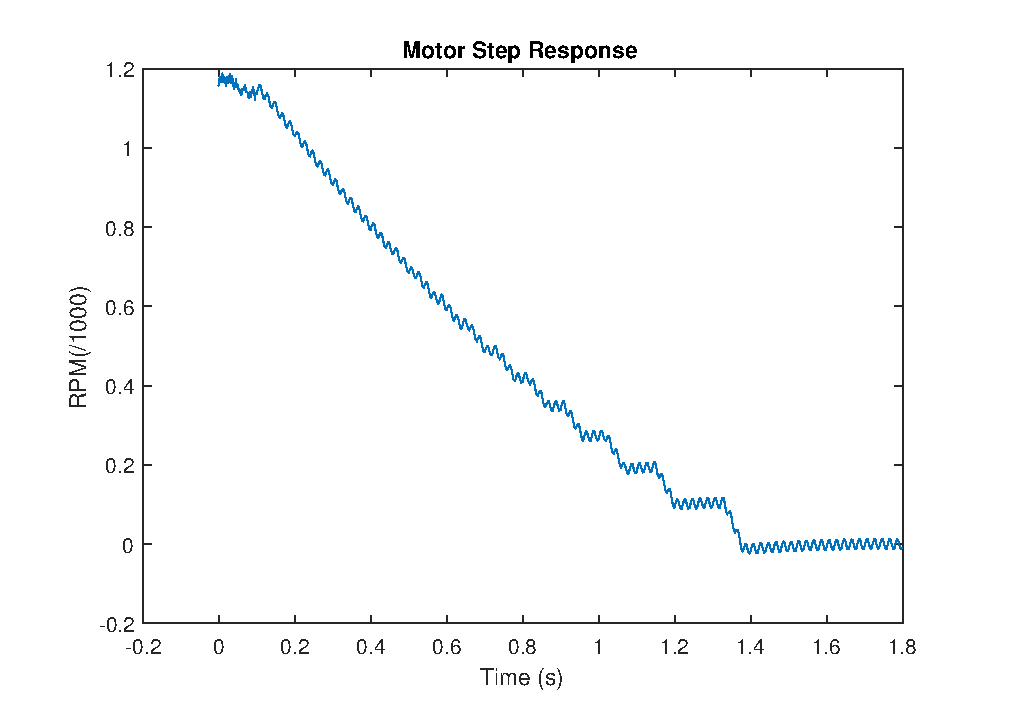
\includegraphics[width=1.2\textwidth]{gfx/Motor_shutoff} %can also be placed in images/example
    \caption{Time Response of the DC motor}
    \label{fig:shutoff}
\end{figure}
From the representation of the data in Figure~\ref{fig:shutoff}, it can be measured that the motor took Approximately 0.77 seconds to reach a speed of 440RPM, A value 63\% from the steady state value. The mechanical time constant $\tau_\ell$ is given by:
\begin{equation}
	\tau_\ell = 0.77s
\end{equation}
\section{Determining K and comparing the model with the results}
Having measured the time constant, the time domain model of the DC motor is in the form:
\begin{align}
	\dot{\omega}(t) &= Ke^{\frac{t}{\tau_\ell} }
\end{align}
Using the value calculated for $\tau_\ell$ and choosing K by means of trial and error, the following model was found to be reasonably close to the measured response:
\begin{align}\label{eq:1}
	K &= 1.2\\
	\dot{\omega}(t) &= 1.2e^{\frac{t}{0.77} }\\
	G(s) &= \frac{1.2}{0.77s+1} 
\end{align}
Refer to Figure~\ref{fig:shutoff_vs_model}, where the time domain model is compared to the measured results. It must be noted that, at this stage in the practical process, the motor was modeled as a function of the input voltage, which was in the order of 0-400V. This model, therefore represents the response to a 400V step in input. It was later found that the motor must be compensated using a duty cycle. Finally, both the reference speed and tachometer output are given in the form:
\begin{align}
1 RPM &= 1mV	
\end{align}
These considerations obviously render the above transfer function unusable (since a plant input in the order of 100 corresponds to an output in the order of 1) and the gain K, must be adjusted before designing the PI controller. It was found that lowering the gain by a factor of 100 yielded an appropriate plant transfer function. By definition, the time constant stays unchanged, regardless of the gain.The transfer function on which the PI controller will be based is therefore given by:
\begin{align}
	\label{eq:motortf}
	G(s) &= \frac{0.012}{0.77s+1} 
\end{align}



\begin{figure}[h]
    \myfloatalign
    \includegraphics[width=1.2\textwidth]{gfx/Motor_shutoff_vs_Time_domain_model} %can also be placed in images/example
    \caption{Simulation of the time domain model compared with Laboratory results}
    \label{fig:shutoff_vs_model}
\end{figure}
\section{Designing the PID}
The following table shows the specifications that the system must adhere to:

\begin{table}[h]
\centering
\caption{Specifications}
\label{tbl:spec}
\begin{tabular}{llll}
\cline{1-2}
\multicolumn{1}{|l|}{\textbf{Parameter}}      & \multicolumn{1}{l|}{\textbf{Maximum Value}} &  &  \\ \cline{1-2}
\multicolumn{1}{|l|}{Steady state error}    & \multicolumn{1}{l|}{1\%}                   &  &  \\ \cline{1-2}
\multicolumn{1}{|l|}{Percent Overshoot(P.O.)} & \multicolumn{1}{l|}{10 \%}                       &  &  \\ \cline{1-2}
\multicolumn{1}{|l|}{Settling time} & \multicolumn{1}{l|}{<2s}                       &  &  \\ \cline{1-2}
                                              &                                             &  & 
\end{tabular}

\end{table}
The transfer function for a PI controller in General is given by:
\begin{equation}\label{eq:2}
	G_{c}(s) = K_{c}+ \frac{K_{i}}{s}
\end{equation}
The equations for Percent overshoot and settling time are given by:
\begin{align} \label{eq:poform}
P.O. &= e^{\left( \frac{-\pi\zeta}{\sqrt{1-\zeta^2}}\right)}
\end{align}
\begin{align}\label{eq:tsform}
T_s &= \frac{4}{\zeta\omega_n}
\end{align}

Furthermore, $\zeta$ and $\omega_n$ can be used to define a desired characteristic equation in the form:

\begin{align} \label{eq:4}
Q(s) &= s^2 + 2\zeta\omega_ns + \omega_n^2
\end{align}

The PI controller design can be summed up as the reconciliation of the desired characteristic equation \ref{eq:4} with the characteristic equation of the system, which is given by:
\begin{align}\label{eq:5}
Q(s) &= G(s)G_c(s) + 1 
\end{align}
With respect to the equations \ref{eq:motortf} and \ref{eq:2}\\
This design is described in the next section.


%----------------------------------------------------------------------------------------

\chapter{Controller Design}
\section{Determining $\zeta$ and $\omega_n$}
Substituting the P.O from Table~\ref{tbl:spec} and solving equation~\ref{eq:poform} yields:
\begin{align}
	\label{eq:zetacalc}
	P.O. &= e^{\left( \frac{-\pi\zeta}{\sqrt{1-\zeta^2}}\right)}\\
	0.1 &= e^{\left( \frac{-\pi\zeta}{\sqrt{1-\zeta^2}}\right)}\\
	\zeta &= 0.5911 \text{ solved numerically} 
\end{align}
Substituting the result of Eq~\ref{eq:zetacalc} and the settling time from Table~\ref{tbl:spec} into eq~\ref{eq:tsform} yields:
\begin{align}
	\label{eq:omegacalc}
	2 &= \frac{4}{\zeta\omega_n} \rvert_{\zeta = 0.5911}\\
	\omega_n &= 3.384
\end{align}

\section{solving for $K_p$ and $K_i$}
Reconciling the compensated transfer function and desired transfer function yields:
\begin{align}
	\label{eq:kpkichar}
Q(s) &= 1 + G_c(s)G(s) \\
Q(s)&= s^2 + 2\zeta\omega_ns + \omega_n^2\\
Q(s) &= s^2 + s(1.298 + 0.012K_p) + 0.012K_i 
\end{align}

By the principle of superposition:
\begin{align}
2\zeta\omega_n &= 1.298 + 0.012K_p \\
\omega_n^2 &= 0.012K_i 
\end{align}
\begin{align}
	\label{eq:}
	K_p &= 255.155\\
	K_i &= 954.288\\
\end{align}
\emph{Note: the values of $K_p$ and $K_i$ seem very high, but this is by design, since the PI controller must have a very high gain, converting an error input in the order of 1V to an output in the order of 100\% }
\section{testing the results}
Figure~\ref{fig:theoplot} was plotted to confirm the calculations. The result was very close to the specification, in the simulation, these results will be tuned, since the specifications are given as upper limits.

\begin{figure}[h]
		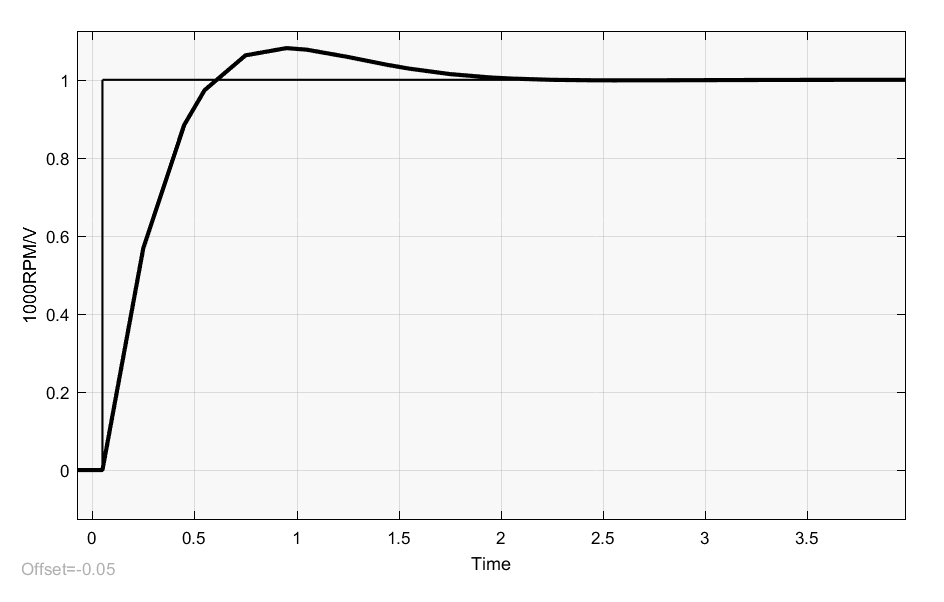
\includegraphics[clip,width=0.7\textwidth]{gfx/calc_plot}%
		\caption{Plot of the transient response of the Caculated system}
\label{fig:theoplot}
\end{figure}


Table~\ref{tbl:theospec} Compares the specification to the theoretical result of the calculated parameters:

\begin{table}[h]
\centering
\caption{Theoretical Results}
\label{tbl:theospec}
\begin{tabular}{llll}
\cline{1-2}
\multicolumn{1}{|l|}{\textbf{Parameter}}      & \multicolumn{1}{l|}{\textbf{Value}} &  &  \\ \cline{1-2}
\multicolumn{1}{|l|}{Steady state error}    & \multicolumn{1}{l|}{0\%}                   &  &  \\ \cline{1-2}
\multicolumn{1}{|l|}{Percent Overshoot(P.O.)} & \multicolumn{1}{l|}{10.5 \%}                       &  &  \\ \cline{1-2}
\multicolumn{1}{|l|}{Settling time} & \multicolumn{1}{l|}{2.2s}                       &  &  \\ \cline{1-2}
                                              &                                             &  & 
\end{tabular}

\end{table}


\chapter{Controller Simulation}
Simulink automates most of the simulation process. Figure~\ref{fig:simblockdiagram} Shows the simple simulation. The simulation was also used to tune the Parameters calculated in the previous section to be well within the specifications. These tuned parameters were implemented using the controller.The parameters after the tuning process are given by:
\begin{description}
	\item[$K_p$] 300 
	\item[$K_i$] 800
\end{description}
\begin{figure}[h]
	\includegraphics[clip,width=1\textwidth]{gfx/sim_Block_Diagram.pdf}%
		\caption{Simulink Block diagram of the compensated plant simulation }
\label{fig:simblockdiagram}
\end{figure}

The simulation in Figure~\ref{fig:simblockdiagram} yields the transient response in Figure~\ref{fig:simbtransplot}

\begin{figure}[h]
		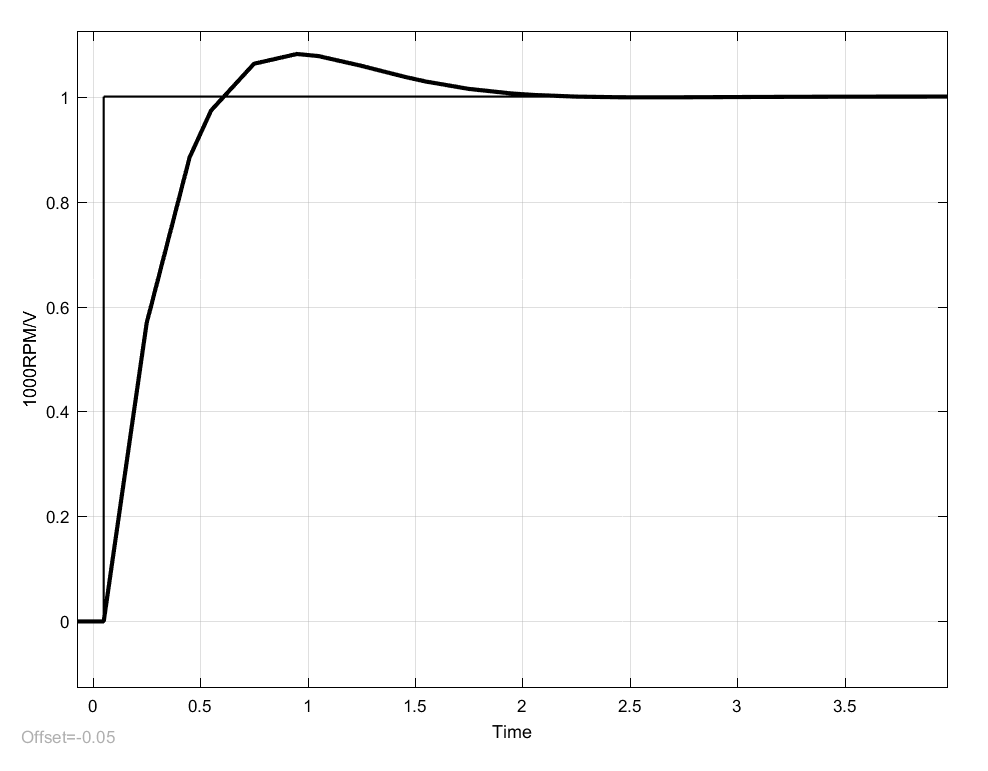
\includegraphics[clip,width=0.7\textwidth]{gfx/sim_plot}%
		\caption{Plot of the transient response of the simulated system}
\label{fig:simbtransplot}
\end{figure}

Table~\ref{tbl:simspec} Compares the specification to the simulated result of the calculated parameters:

\begin{table}[h]
\centering
\caption{Simulated Results}
\label{tbl:simspec}
\begin{tabular}{llll}
\cline{1-2}
\multicolumn{1}{|l|}{\textbf{Parameter}}      & \multicolumn{1}{l|}{\textbf{Value}} &  &  \\ \cline{1-2}
\multicolumn{1}{|l|}{Steady state error}    & \multicolumn{1}{l|}{0\%}                   &  &  \\ \cline{1-2}
\multicolumn{1}{|l|}{Percent Overshoot(P.O.)} & \multicolumn{1}{l|}{8.1 \%}                       &  &  \\ \cline{1-2}
\multicolumn{1}{|l|}{Settling time} & \multicolumn{1}{l|}{2s}                       &  &  \\ \cline{1-2}
                                              &                                             &  & 
\end{tabular}

\end{table}


\chapter{Practical Implementation}
Having calculated and simulated the PI compensator, it was implemented on an ARM microcontroller and connected to a driver circuit. The microcontroller was also configured to log the following data:
\begin{itemize}
	\item The desired set point (Volt)
	\item Tachometer output (Volt)
	\item Error (Volt)
	\item Duty cycle(\%)
\end{itemize}
The output used to plot Figure~\ref{fig:practrans} was prepared for plotting using the python script included in Appendix~\hyperref[apx:B]{B}. A step input of 1V was used, making the setpoint for the controller to track 1000RPM. 
\begin{figure}[h]
% GNUPLOT: LaTeX picture
\setlength{\unitlength}{0.240900pt}
\ifx\plotpoint\undefined\newsavebox{\plotpoint}\fi
\begin{picture}(1500,900)(0,0)
\sbox{\plotpoint}{\rule[-0.200pt]{0.400pt}{0.400pt}}%
\put(151.0,131.0){\rule[-0.200pt]{310.279pt}{0.400pt}}
\put(151.0,131.0){\rule[-0.200pt]{4.818pt}{0.400pt}}
\put(131,131){\makebox(0,0)[r]{$0$}}
\put(1419.0,131.0){\rule[-0.200pt]{4.818pt}{0.400pt}}
\put(151.0,252.0){\rule[-0.200pt]{310.279pt}{0.400pt}}
\put(151.0,252.0){\rule[-0.200pt]{4.818pt}{0.400pt}}
\put(131,252){\makebox(0,0)[r]{$0.2$}}
\put(1419.0,252.0){\rule[-0.200pt]{4.818pt}{0.400pt}}
\put(151.0,374.0){\rule[-0.200pt]{310.279pt}{0.400pt}}
\put(151.0,374.0){\rule[-0.200pt]{4.818pt}{0.400pt}}
\put(131,374){\makebox(0,0)[r]{$0.4$}}
\put(1419.0,374.0){\rule[-0.200pt]{4.818pt}{0.400pt}}
\put(151.0,495.0){\rule[-0.200pt]{310.279pt}{0.400pt}}
\put(151.0,495.0){\rule[-0.200pt]{4.818pt}{0.400pt}}
\put(131,495){\makebox(0,0)[r]{$0.6$}}
\put(1419.0,495.0){\rule[-0.200pt]{4.818pt}{0.400pt}}
\put(151.0,616.0){\rule[-0.200pt]{310.279pt}{0.400pt}}
\put(151.0,616.0){\rule[-0.200pt]{4.818pt}{0.400pt}}
\put(131,616){\makebox(0,0)[r]{$0.8$}}
\put(1419.0,616.0){\rule[-0.200pt]{4.818pt}{0.400pt}}
\put(151.0,738.0){\rule[-0.200pt]{310.279pt}{0.400pt}}
\put(151.0,738.0){\rule[-0.200pt]{4.818pt}{0.400pt}}
\put(131,738){\makebox(0,0)[r]{$1$}}
\put(1419.0,738.0){\rule[-0.200pt]{4.818pt}{0.400pt}}
\put(151.0,859.0){\rule[-0.200pt]{310.279pt}{0.400pt}}
\put(151.0,859.0){\rule[-0.200pt]{4.818pt}{0.400pt}}
\put(131,859){\makebox(0,0)[r]{$1.2$}}
\put(1419.0,859.0){\rule[-0.200pt]{4.818pt}{0.400pt}}
\put(151.0,131.0){\rule[-0.200pt]{0.400pt}{175.375pt}}
\put(151.0,131.0){\rule[-0.200pt]{0.400pt}{4.818pt}}
\put(151,90){\makebox(0,0){$0$}}
\put(151.0,839.0){\rule[-0.200pt]{0.400pt}{4.818pt}}
\put(409.0,131.0){\rule[-0.200pt]{0.400pt}{175.375pt}}
\put(409.0,131.0){\rule[-0.200pt]{0.400pt}{4.818pt}}
\put(409,90){\makebox(0,0){$2$}}
\put(409.0,839.0){\rule[-0.200pt]{0.400pt}{4.818pt}}
\put(666.0,131.0){\rule[-0.200pt]{0.400pt}{175.375pt}}
\put(666.0,131.0){\rule[-0.200pt]{0.400pt}{4.818pt}}
\put(666,90){\makebox(0,0){$4$}}
\put(666.0,839.0){\rule[-0.200pt]{0.400pt}{4.818pt}}
\put(924.0,131.0){\rule[-0.200pt]{0.400pt}{175.375pt}}
\put(924.0,131.0){\rule[-0.200pt]{0.400pt}{4.818pt}}
\put(924,90){\makebox(0,0){$6$}}
\put(924.0,839.0){\rule[-0.200pt]{0.400pt}{4.818pt}}
\put(1181.0,131.0){\rule[-0.200pt]{0.400pt}{175.375pt}}
\put(1181.0,131.0){\rule[-0.200pt]{0.400pt}{4.818pt}}
\put(1181,90){\makebox(0,0){$8$}}
\put(1181.0,839.0){\rule[-0.200pt]{0.400pt}{4.818pt}}
\put(1439.0,131.0){\rule[-0.200pt]{0.400pt}{175.375pt}}
\put(1439.0,131.0){\rule[-0.200pt]{0.400pt}{4.818pt}}
\put(1439,90){\makebox(0,0){$10$}}
\put(1439.0,839.0){\rule[-0.200pt]{0.400pt}{4.818pt}}
\put(151.0,131.0){\rule[-0.200pt]{0.400pt}{175.375pt}}
\put(151.0,131.0){\rule[-0.200pt]{310.279pt}{0.400pt}}
\put(1439.0,131.0){\rule[-0.200pt]{0.400pt}{175.375pt}}
\put(151.0,859.0){\rule[-0.200pt]{310.279pt}{0.400pt}}
\put(30,495){\makebox(0,0){\rotatebox{90}{Voltage/RPM}}}
\put(795,29){\makebox(0,0){Time}}
\put(151,201){\usebox{\plotpoint}}
\multiput(151.58,201.00)(0.493,0.853){23}{\rule{0.119pt}{0.777pt}}
\multiput(150.17,201.00)(13.000,20.387){2}{\rule{0.400pt}{0.388pt}}
\multiput(164.58,223.00)(0.493,0.695){23}{\rule{0.119pt}{0.654pt}}
\multiput(163.17,223.00)(13.000,16.643){2}{\rule{0.400pt}{0.327pt}}
\multiput(177.58,241.00)(0.493,0.933){23}{\rule{0.119pt}{0.838pt}}
\multiput(176.17,241.00)(13.000,22.260){2}{\rule{0.400pt}{0.419pt}}
\multiput(190.58,265.00)(0.493,0.933){23}{\rule{0.119pt}{0.838pt}}
\multiput(189.17,265.00)(13.000,22.260){2}{\rule{0.400pt}{0.419pt}}
\multiput(203.58,289.00)(0.492,1.056){21}{\rule{0.119pt}{0.933pt}}
\multiput(202.17,289.00)(12.000,23.063){2}{\rule{0.400pt}{0.467pt}}
\multiput(215.58,314.00)(0.493,1.012){23}{\rule{0.119pt}{0.900pt}}
\multiput(214.17,314.00)(13.000,24.132){2}{\rule{0.400pt}{0.450pt}}
\multiput(228.58,340.00)(0.493,0.972){23}{\rule{0.119pt}{0.869pt}}
\multiput(227.17,340.00)(13.000,23.196){2}{\rule{0.400pt}{0.435pt}}
\multiput(241.58,365.00)(0.493,3.431){23}{\rule{0.119pt}{2.777pt}}
\multiput(240.17,365.00)(13.000,81.236){2}{\rule{0.400pt}{1.388pt}}
\multiput(254.58,452.00)(0.493,1.052){23}{\rule{0.119pt}{0.931pt}}
\multiput(253.17,452.00)(13.000,25.068){2}{\rule{0.400pt}{0.465pt}}
\multiput(267.58,479.00)(0.493,1.091){23}{\rule{0.119pt}{0.962pt}}
\multiput(266.17,479.00)(13.000,26.004){2}{\rule{0.400pt}{0.481pt}}
\multiput(280.58,507.00)(0.493,1.131){23}{\rule{0.119pt}{0.992pt}}
\multiput(279.17,507.00)(13.000,26.940){2}{\rule{0.400pt}{0.496pt}}
\multiput(293.58,536.00)(0.493,1.091){23}{\rule{0.119pt}{0.962pt}}
\multiput(292.17,536.00)(13.000,26.004){2}{\rule{0.400pt}{0.481pt}}
\multiput(306.58,564.00)(0.492,1.272){21}{\rule{0.119pt}{1.100pt}}
\multiput(305.17,564.00)(12.000,27.717){2}{\rule{0.400pt}{0.550pt}}
\multiput(318.58,594.00)(0.493,1.171){23}{\rule{0.119pt}{1.023pt}}
\multiput(317.17,594.00)(13.000,27.877){2}{\rule{0.400pt}{0.512pt}}
\multiput(331.58,624.00)(0.493,1.131){23}{\rule{0.119pt}{0.992pt}}
\multiput(330.17,624.00)(13.000,26.940){2}{\rule{0.400pt}{0.496pt}}
\multiput(344.58,653.00)(0.493,1.131){23}{\rule{0.119pt}{0.992pt}}
\multiput(343.17,653.00)(13.000,26.940){2}{\rule{0.400pt}{0.496pt}}
\multiput(357.58,682.00)(0.493,0.655){23}{\rule{0.119pt}{0.623pt}}
\multiput(356.17,682.00)(13.000,15.707){2}{\rule{0.400pt}{0.312pt}}
\multiput(370.00,699.58)(0.497,0.493){23}{\rule{0.500pt}{0.119pt}}
\multiput(370.00,698.17)(11.962,13.000){2}{\rule{0.250pt}{0.400pt}}
\multiput(383.00,712.58)(0.652,0.491){17}{\rule{0.620pt}{0.118pt}}
\multiput(383.00,711.17)(11.713,10.000){2}{\rule{0.310pt}{0.400pt}}
\multiput(396.00,722.59)(0.728,0.489){15}{\rule{0.678pt}{0.118pt}}
\multiput(396.00,721.17)(11.593,9.000){2}{\rule{0.339pt}{0.400pt}}
\multiput(409.00,731.59)(0.758,0.488){13}{\rule{0.700pt}{0.117pt}}
\multiput(409.00,730.17)(10.547,8.000){2}{\rule{0.350pt}{0.400pt}}
\multiput(421.00,739.58)(0.590,0.492){19}{\rule{0.573pt}{0.118pt}}
\multiput(421.00,738.17)(11.811,11.000){2}{\rule{0.286pt}{0.400pt}}
\multiput(434.00,750.59)(1.123,0.482){9}{\rule{0.967pt}{0.116pt}}
\multiput(434.00,749.17)(10.994,6.000){2}{\rule{0.483pt}{0.400pt}}
\multiput(447.00,756.60)(1.797,0.468){5}{\rule{1.400pt}{0.113pt}}
\multiput(447.00,755.17)(10.094,4.000){2}{\rule{0.700pt}{0.400pt}}
\multiput(460.00,760.61)(2.695,0.447){3}{\rule{1.833pt}{0.108pt}}
\multiput(460.00,759.17)(9.195,3.000){2}{\rule{0.917pt}{0.400pt}}
\multiput(473.00,763.61)(2.695,0.447){3}{\rule{1.833pt}{0.108pt}}
\multiput(473.00,762.17)(9.195,3.000){2}{\rule{0.917pt}{0.400pt}}
\multiput(486.00,766.59)(1.378,0.477){7}{\rule{1.140pt}{0.115pt}}
\multiput(486.00,765.17)(10.634,5.000){2}{\rule{0.570pt}{0.400pt}}
\multiput(499.58,763.30)(0.493,-2.241){23}{\rule{0.119pt}{1.854pt}}
\multiput(498.17,767.15)(13.000,-53.152){2}{\rule{0.400pt}{0.927pt}}
\multiput(512.00,714.60)(1.797,0.468){5}{\rule{1.400pt}{0.113pt}}
\multiput(512.00,713.17)(10.094,4.000){2}{\rule{0.700pt}{0.400pt}}
\multiput(525.00,718.61)(2.472,0.447){3}{\rule{1.700pt}{0.108pt}}
\multiput(525.00,717.17)(8.472,3.000){2}{\rule{0.850pt}{0.400pt}}
\put(537,721.17){\rule{2.700pt}{0.400pt}}
\multiput(537.00,720.17)(7.396,2.000){2}{\rule{1.350pt}{0.400pt}}
\put(550,722.67){\rule{3.132pt}{0.400pt}}
\multiput(550.00,722.17)(6.500,1.000){2}{\rule{1.566pt}{0.400pt}}
\put(563,722.67){\rule{3.132pt}{0.400pt}}
\multiput(563.00,723.17)(6.500,-1.000){2}{\rule{1.566pt}{0.400pt}}
\put(589,723.17){\rule{2.700pt}{0.400pt}}
\multiput(589.00,722.17)(7.396,2.000){2}{\rule{1.350pt}{0.400pt}}
\put(576.0,723.0){\rule[-0.200pt]{3.132pt}{0.400pt}}
\put(628,723.67){\rule{2.891pt}{0.400pt}}
\multiput(628.00,724.17)(6.000,-1.000){2}{\rule{1.445pt}{0.400pt}}
\put(602.0,725.0){\rule[-0.200pt]{6.263pt}{0.400pt}}
\put(653,723.67){\rule{3.132pt}{0.400pt}}
\multiput(653.00,723.17)(6.500,1.000){2}{\rule{1.566pt}{0.400pt}}
\put(640.0,724.0){\rule[-0.200pt]{3.132pt}{0.400pt}}
\put(692,723.67){\rule{3.132pt}{0.400pt}}
\multiput(692.00,724.17)(6.500,-1.000){2}{\rule{1.566pt}{0.400pt}}
\put(705,723.67){\rule{3.132pt}{0.400pt}}
\multiput(705.00,723.17)(6.500,1.000){2}{\rule{1.566pt}{0.400pt}}
\put(718,724.67){\rule{3.132pt}{0.400pt}}
\multiput(718.00,724.17)(6.500,1.000){2}{\rule{1.566pt}{0.400pt}}
\put(731,725.67){\rule{2.891pt}{0.400pt}}
\multiput(731.00,725.17)(6.000,1.000){2}{\rule{1.445pt}{0.400pt}}
\put(743,726.67){\rule{3.132pt}{0.400pt}}
\multiput(743.00,726.17)(6.500,1.000){2}{\rule{1.566pt}{0.400pt}}
\put(756,726.67){\rule{3.132pt}{0.400pt}}
\multiput(756.00,727.17)(6.500,-1.000){2}{\rule{1.566pt}{0.400pt}}
\put(769,725.67){\rule{3.132pt}{0.400pt}}
\multiput(769.00,726.17)(6.500,-1.000){2}{\rule{1.566pt}{0.400pt}}
\put(782,724.67){\rule{3.132pt}{0.400pt}}
\multiput(782.00,725.17)(6.500,-1.000){2}{\rule{1.566pt}{0.400pt}}
\put(795,724.67){\rule{3.132pt}{0.400pt}}
\multiput(795.00,724.17)(6.500,1.000){2}{\rule{1.566pt}{0.400pt}}
\put(808,725.67){\rule{3.132pt}{0.400pt}}
\multiput(808.00,725.17)(6.500,1.000){2}{\rule{1.566pt}{0.400pt}}
\put(821,726.67){\rule{3.132pt}{0.400pt}}
\multiput(821.00,726.17)(6.500,1.000){2}{\rule{1.566pt}{0.400pt}}
\put(834,727.67){\rule{3.132pt}{0.400pt}}
\multiput(834.00,727.17)(6.500,1.000){2}{\rule{1.566pt}{0.400pt}}
\put(666.0,725.0){\rule[-0.200pt]{6.263pt}{0.400pt}}
\put(859,728.67){\rule{3.132pt}{0.400pt}}
\multiput(859.00,728.17)(6.500,1.000){2}{\rule{1.566pt}{0.400pt}}
\put(872,729.67){\rule{3.132pt}{0.400pt}}
\multiput(872.00,729.17)(6.500,1.000){2}{\rule{1.566pt}{0.400pt}}
\put(885,731.17){\rule{2.700pt}{0.400pt}}
\multiput(885.00,730.17)(7.396,2.000){2}{\rule{1.350pt}{0.400pt}}
\put(898,733.17){\rule{2.700pt}{0.400pt}}
\multiput(898.00,732.17)(7.396,2.000){2}{\rule{1.350pt}{0.400pt}}
\put(847.0,729.0){\rule[-0.200pt]{2.891pt}{0.400pt}}
\put(937,734.67){\rule{3.132pt}{0.400pt}}
\multiput(937.00,734.17)(6.500,1.000){2}{\rule{1.566pt}{0.400pt}}
\put(950,736.17){\rule{2.500pt}{0.400pt}}
\multiput(950.00,735.17)(6.811,2.000){2}{\rule{1.250pt}{0.400pt}}
\put(962,737.67){\rule{3.132pt}{0.400pt}}
\multiput(962.00,737.17)(6.500,1.000){2}{\rule{1.566pt}{0.400pt}}
\put(975,738.67){\rule{3.132pt}{0.400pt}}
\multiput(975.00,738.17)(6.500,1.000){2}{\rule{1.566pt}{0.400pt}}
\put(988,738.67){\rule{3.132pt}{0.400pt}}
\multiput(988.00,739.17)(6.500,-1.000){2}{\rule{1.566pt}{0.400pt}}
\put(911.0,735.0){\rule[-0.200pt]{6.263pt}{0.400pt}}
\put(1014,738.67){\rule{3.132pt}{0.400pt}}
\multiput(1014.00,738.17)(6.500,1.000){2}{\rule{1.566pt}{0.400pt}}
\put(1001.0,739.0){\rule[-0.200pt]{3.132pt}{0.400pt}}
\put(1053,738.67){\rule{2.891pt}{0.400pt}}
\multiput(1053.00,739.17)(6.000,-1.000){2}{\rule{1.445pt}{0.400pt}}
\put(1065,737.67){\rule{3.132pt}{0.400pt}}
\multiput(1065.00,738.17)(6.500,-1.000){2}{\rule{1.566pt}{0.400pt}}
\put(1078,737.67){\rule{3.132pt}{0.400pt}}
\multiput(1078.00,737.17)(6.500,1.000){2}{\rule{1.566pt}{0.400pt}}
\put(1091,737.67){\rule{3.132pt}{0.400pt}}
\multiput(1091.00,738.17)(6.500,-1.000){2}{\rule{1.566pt}{0.400pt}}
\put(1104,736.67){\rule{3.132pt}{0.400pt}}
\multiput(1104.00,737.17)(6.500,-1.000){2}{\rule{1.566pt}{0.400pt}}
\put(1117,735.67){\rule{3.132pt}{0.400pt}}
\multiput(1117.00,736.17)(6.500,-1.000){2}{\rule{1.566pt}{0.400pt}}
\put(1027.0,740.0){\rule[-0.200pt]{6.263pt}{0.400pt}}
\put(1143,734.17){\rule{2.700pt}{0.400pt}}
\multiput(1143.00,735.17)(7.396,-2.000){2}{\rule{1.350pt}{0.400pt}}
\put(1156,732.67){\rule{3.132pt}{0.400pt}}
\multiput(1156.00,733.17)(6.500,-1.000){2}{\rule{1.566pt}{0.400pt}}
\put(1130.0,736.0){\rule[-0.200pt]{3.132pt}{0.400pt}}
\put(1207,731.17){\rule{2.700pt}{0.400pt}}
\multiput(1207.00,732.17)(7.396,-2.000){2}{\rule{1.350pt}{0.400pt}}
\put(1220,729.67){\rule{3.132pt}{0.400pt}}
\multiput(1220.00,730.17)(6.500,-1.000){2}{\rule{1.566pt}{0.400pt}}
\put(1233,728.17){\rule{2.700pt}{0.400pt}}
\multiput(1233.00,729.17)(7.396,-2.000){2}{\rule{1.350pt}{0.400pt}}
\put(1246,727.67){\rule{3.132pt}{0.400pt}}
\multiput(1246.00,727.17)(6.500,1.000){2}{\rule{1.566pt}{0.400pt}}
\put(1259,728.67){\rule{3.132pt}{0.400pt}}
\multiput(1259.00,728.17)(6.500,1.000){2}{\rule{1.566pt}{0.400pt}}
\put(1272,728.17){\rule{2.500pt}{0.400pt}}
\multiput(1272.00,729.17)(6.811,-2.000){2}{\rule{1.250pt}{0.400pt}}
\put(1169.0,733.0){\rule[-0.200pt]{9.154pt}{0.400pt}}
\put(1323,726.67){\rule{3.132pt}{0.400pt}}
\multiput(1323.00,727.17)(6.500,-1.000){2}{\rule{1.566pt}{0.400pt}}
\put(1336,725.67){\rule{3.132pt}{0.400pt}}
\multiput(1336.00,726.17)(6.500,-1.000){2}{\rule{1.566pt}{0.400pt}}
\put(1349,726.17){\rule{2.700pt}{0.400pt}}
\multiput(1349.00,725.17)(7.396,2.000){2}{\rule{1.350pt}{0.400pt}}
\put(1362,727.67){\rule{3.132pt}{0.400pt}}
\multiput(1362.00,727.17)(6.500,1.000){2}{\rule{1.566pt}{0.400pt}}
\put(1284.0,728.0){\rule[-0.200pt]{9.395pt}{0.400pt}}
\put(1387,727.67){\rule{3.132pt}{0.400pt}}
\multiput(1387.00,728.17)(6.500,-1.000){2}{\rule{1.566pt}{0.400pt}}
\put(1375.0,729.0){\rule[-0.200pt]{2.891pt}{0.400pt}}
\put(1413,727.67){\rule{3.132pt}{0.400pt}}
\multiput(1413.00,727.17)(6.500,1.000){2}{\rule{1.566pt}{0.400pt}}
\put(1426,727.67){\rule{3.132pt}{0.400pt}}
\multiput(1426.00,728.17)(6.500,-1.000){2}{\rule{1.566pt}{0.400pt}}
\put(1400.0,728.0){\rule[-0.200pt]{3.132pt}{0.400pt}}
\put(1439,728){\usebox{\plotpoint}}
\put(151.0,131.0){\rule[-0.200pt]{0.400pt}{175.375pt}}
\put(151.0,131.0){\rule[-0.200pt]{310.279pt}{0.400pt}}
\put(1439.0,131.0){\rule[-0.200pt]{0.400pt}{175.375pt}}
\put(151.0,859.0){\rule[-0.200pt]{310.279pt}{0.400pt}}
\end{picture}
\begin{picture}(1500,900)(0,0)
\put(151.0,180.0){\rule[-0.200pt]{310.279pt}{0.400pt}}
\put(151.0,180.0){\rule[-0.200pt]{4.818pt}{0.400pt}}
\put(131,180){\makebox(0,0)[r]{$0.2$}}
\put(1419.0,180.0){\rule[-0.200pt]{4.818pt}{0.400pt}}
\put(151.0,301.0){\rule[-0.200pt]{310.279pt}{0.400pt}}
\put(151.0,301.0){\rule[-0.200pt]{4.818pt}{0.400pt}}
\put(131,301){\makebox(0,0)[r]{$0.4$}}
\put(1419.0,301.0){\rule[-0.200pt]{4.818pt}{0.400pt}}
\put(151.0,422.0){\rule[-0.200pt]{310.279pt}{0.400pt}}
\put(151.0,422.0){\rule[-0.200pt]{4.818pt}{0.400pt}}
\put(131,422){\makebox(0,0)[r]{$0.6$}}
\put(1419.0,422.0){\rule[-0.200pt]{4.818pt}{0.400pt}}
\put(151.0,544.0){\rule[-0.200pt]{310.279pt}{0.400pt}}
\put(151.0,544.0){\rule[-0.200pt]{4.818pt}{0.400pt}}
\put(131,544){\makebox(0,0)[r]{$0.8$}}
\put(1419.0,544.0){\rule[-0.200pt]{4.818pt}{0.400pt}}
\put(151.0,665.0){\rule[-0.200pt]{310.279pt}{0.400pt}}
\put(151.0,665.0){\rule[-0.200pt]{4.818pt}{0.400pt}}
\put(131,665){\makebox(0,0)[r]{$1$}}
\put(1419.0,665.0){\rule[-0.200pt]{4.818pt}{0.400pt}}
\put(151.0,786.0){\rule[-0.200pt]{310.279pt}{0.400pt}}
\put(151.0,786.0){\rule[-0.200pt]{4.818pt}{0.400pt}}
\put(131,786){\makebox(0,0)[r]{$1.2$}}
\put(1419.0,786.0){\rule[-0.200pt]{4.818pt}{0.400pt}}
\put(151.0,131.0){\rule[-0.200pt]{0.400pt}{175.375pt}}
\put(151.0,131.0){\rule[-0.200pt]{0.400pt}{4.818pt}}
\put(151,90){\makebox(0,0){$0$}}
\put(151.0,839.0){\rule[-0.200pt]{0.400pt}{4.818pt}}
\put(409.0,131.0){\rule[-0.200pt]{0.400pt}{175.375pt}}
\put(409.0,131.0){\rule[-0.200pt]{0.400pt}{4.818pt}}
\put(409,90){\makebox(0,0){$2$}}
\put(409.0,839.0){\rule[-0.200pt]{0.400pt}{4.818pt}}
\put(666.0,131.0){\rule[-0.200pt]{0.400pt}{175.375pt}}
\put(666.0,131.0){\rule[-0.200pt]{0.400pt}{4.818pt}}
\put(666,90){\makebox(0,0){$4$}}
\put(666.0,839.0){\rule[-0.200pt]{0.400pt}{4.818pt}}
\put(924.0,131.0){\rule[-0.200pt]{0.400pt}{175.375pt}}
\put(924.0,131.0){\rule[-0.200pt]{0.400pt}{4.818pt}}
\put(924,90){\makebox(0,0){$6$}}
\put(924.0,839.0){\rule[-0.200pt]{0.400pt}{4.818pt}}
\put(1181.0,131.0){\rule[-0.200pt]{0.400pt}{175.375pt}}
\put(1181.0,131.0){\rule[-0.200pt]{0.400pt}{4.818pt}}
\put(1181,90){\makebox(0,0){$8$}}
\put(1181.0,839.0){\rule[-0.200pt]{0.400pt}{4.818pt}}
\put(1439.0,131.0){\rule[-0.200pt]{0.400pt}{175.375pt}}
\put(1439.0,131.0){\rule[-0.200pt]{0.400pt}{4.818pt}}
\put(1439,90){\makebox(0,0){$10$}}
\put(1439.0,839.0){\rule[-0.200pt]{0.400pt}{4.818pt}}
\put(151.0,131.0){\rule[-0.200pt]{0.400pt}{175.375pt}}
\put(151.0,131.0){\rule[-0.200pt]{310.279pt}{0.400pt}}
\put(1439.0,131.0){\rule[-0.200pt]{0.400pt}{175.375pt}}
\put(151.0,859.0){\rule[-0.200pt]{310.279pt}{0.400pt}}
\put(30,495){\makebox(0,0){\rotatebox{90}{Voltage/RPM}}}
\put(795,29){\makebox(0,0){Time}}
\multiput(153.58,131.00)(0.492,0.873){19}{\rule{0.118pt}{0.791pt}}
\multiput(152.17,131.00)(11.000,17.358){2}{\rule{0.400pt}{0.395pt}}
\multiput(164.58,150.00)(0.493,0.695){23}{\rule{0.119pt}{0.654pt}}
\multiput(163.17,150.00)(13.000,16.643){2}{\rule{0.400pt}{0.327pt}}
\multiput(177.58,168.00)(0.493,0.933){23}{\rule{0.119pt}{0.838pt}}
\multiput(176.17,168.00)(13.000,22.260){2}{\rule{0.400pt}{0.419pt}}
\multiput(190.58,192.00)(0.493,0.933){23}{\rule{0.119pt}{0.838pt}}
\multiput(189.17,192.00)(13.000,22.260){2}{\rule{0.400pt}{0.419pt}}
\multiput(203.58,216.00)(0.492,1.099){21}{\rule{0.119pt}{0.967pt}}
\multiput(202.17,216.00)(12.000,23.994){2}{\rule{0.400pt}{0.483pt}}
\multiput(215.58,242.00)(0.493,0.972){23}{\rule{0.119pt}{0.869pt}}
\multiput(214.17,242.00)(13.000,23.196){2}{\rule{0.400pt}{0.435pt}}
\multiput(228.58,267.00)(0.493,1.012){23}{\rule{0.119pt}{0.900pt}}
\multiput(227.17,267.00)(13.000,24.132){2}{\rule{0.400pt}{0.450pt}}
\multiput(241.58,293.00)(0.493,3.391){23}{\rule{0.119pt}{2.746pt}}
\multiput(240.17,293.00)(13.000,80.300){2}{\rule{0.400pt}{1.373pt}}
\multiput(254.58,379.00)(0.493,1.052){23}{\rule{0.119pt}{0.931pt}}
\multiput(253.17,379.00)(13.000,25.068){2}{\rule{0.400pt}{0.465pt}}
\multiput(267.58,406.00)(0.493,1.091){23}{\rule{0.119pt}{0.962pt}}
\multiput(266.17,406.00)(13.000,26.004){2}{\rule{0.400pt}{0.481pt}}
\multiput(280.58,434.00)(0.493,1.131){23}{\rule{0.119pt}{0.992pt}}
\multiput(279.17,434.00)(13.000,26.940){2}{\rule{0.400pt}{0.496pt}}
\multiput(293.58,463.00)(0.493,1.131){23}{\rule{0.119pt}{0.992pt}}
\multiput(292.17,463.00)(13.000,26.940){2}{\rule{0.400pt}{0.496pt}}
\multiput(306.58,492.00)(0.492,1.229){21}{\rule{0.119pt}{1.067pt}}
\multiput(305.17,492.00)(12.000,26.786){2}{\rule{0.400pt}{0.533pt}}
\multiput(318.58,521.00)(0.493,1.171){23}{\rule{0.119pt}{1.023pt}}
\multiput(317.17,521.00)(13.000,27.877){2}{\rule{0.400pt}{0.512pt}}
\multiput(331.58,551.00)(0.493,1.131){23}{\rule{0.119pt}{0.992pt}}
\multiput(330.17,551.00)(13.000,26.940){2}{\rule{0.400pt}{0.496pt}}
\multiput(344.58,580.00)(0.493,1.131){23}{\rule{0.119pt}{0.992pt}}
\multiput(343.17,580.00)(13.000,26.940){2}{\rule{0.400pt}{0.496pt}}
\multiput(357.58,609.00)(0.493,0.655){23}{\rule{0.119pt}{0.623pt}}
\multiput(356.17,609.00)(13.000,15.707){2}{\rule{0.400pt}{0.312pt}}
\multiput(370.00,626.58)(0.497,0.493){23}{\rule{0.500pt}{0.119pt}}
\multiput(370.00,625.17)(11.962,13.000){2}{\rule{0.250pt}{0.400pt}}
\multiput(383.00,639.58)(0.652,0.491){17}{\rule{0.620pt}{0.118pt}}
\multiput(383.00,638.17)(11.713,10.000){2}{\rule{0.310pt}{0.400pt}}
\multiput(396.00,649.59)(0.728,0.489){15}{\rule{0.678pt}{0.118pt}}
\multiput(396.00,648.17)(11.593,9.000){2}{\rule{0.339pt}{0.400pt}}
\multiput(409.00,658.59)(0.758,0.488){13}{\rule{0.700pt}{0.117pt}}
\multiput(409.00,657.17)(10.547,8.000){2}{\rule{0.350pt}{0.400pt}}
\multiput(421.00,666.58)(0.590,0.492){19}{\rule{0.573pt}{0.118pt}}
\multiput(421.00,665.17)(11.811,11.000){2}{\rule{0.286pt}{0.400pt}}
\multiput(434.00,677.59)(1.123,0.482){9}{\rule{0.967pt}{0.116pt}}
\multiput(434.00,676.17)(10.994,6.000){2}{\rule{0.483pt}{0.400pt}}
\multiput(447.00,683.60)(1.797,0.468){5}{\rule{1.400pt}{0.113pt}}
\multiput(447.00,682.17)(10.094,4.000){2}{\rule{0.700pt}{0.400pt}}
\multiput(460.00,687.61)(2.695,0.447){3}{\rule{1.833pt}{0.108pt}}
\multiput(460.00,686.17)(9.195,3.000){2}{\rule{0.917pt}{0.400pt}}
\multiput(473.00,690.61)(2.695,0.447){3}{\rule{1.833pt}{0.108pt}}
\multiput(473.00,689.17)(9.195,3.000){2}{\rule{0.917pt}{0.400pt}}
\multiput(486.00,693.59)(1.378,0.477){7}{\rule{1.140pt}{0.115pt}}
\multiput(486.00,692.17)(10.634,5.000){2}{\rule{0.570pt}{0.400pt}}
\multiput(499.58,690.30)(0.493,-2.241){23}{\rule{0.119pt}{1.854pt}}
\multiput(498.17,694.15)(13.000,-53.152){2}{\rule{0.400pt}{0.927pt}}
\multiput(512.00,641.60)(1.797,0.468){5}{\rule{1.400pt}{0.113pt}}
\multiput(512.00,640.17)(10.094,4.000){2}{\rule{0.700pt}{0.400pt}}
\multiput(525.00,645.61)(2.472,0.447){3}{\rule{1.700pt}{0.108pt}}
\multiput(525.00,644.17)(8.472,3.000){2}{\rule{0.850pt}{0.400pt}}
\put(537,648.17){\rule{2.700pt}{0.400pt}}
\multiput(537.00,647.17)(7.396,2.000){2}{\rule{1.350pt}{0.400pt}}
\put(550,649.67){\rule{3.132pt}{0.400pt}}
\multiput(550.00,649.17)(6.500,1.000){2}{\rule{1.566pt}{0.400pt}}
\put(589,650.67){\rule{3.132pt}{0.400pt}}
\multiput(589.00,650.17)(6.500,1.000){2}{\rule{1.566pt}{0.400pt}}
\put(602,651.67){\rule{3.132pt}{0.400pt}}
\multiput(602.00,651.17)(6.500,1.000){2}{\rule{1.566pt}{0.400pt}}
\put(615,651.67){\rule{3.132pt}{0.400pt}}
\multiput(615.00,652.17)(6.500,-1.000){2}{\rule{1.566pt}{0.400pt}}
\put(563.0,651.0){\rule[-0.200pt]{6.263pt}{0.400pt}}
\put(718,651.67){\rule{3.132pt}{0.400pt}}
\multiput(718.00,651.17)(6.500,1.000){2}{\rule{1.566pt}{0.400pt}}
\put(731,653.17){\rule{2.500pt}{0.400pt}}
\multiput(731.00,652.17)(6.811,2.000){2}{\rule{1.250pt}{0.400pt}}
\put(628.0,652.0){\rule[-0.200pt]{21.681pt}{0.400pt}}
\put(769,653.17){\rule{2.700pt}{0.400pt}}
\multiput(769.00,654.17)(7.396,-2.000){2}{\rule{1.350pt}{0.400pt}}
\put(743.0,655.0){\rule[-0.200pt]{6.263pt}{0.400pt}}
\put(808,653.17){\rule{2.700pt}{0.400pt}}
\multiput(808.00,652.17)(7.396,2.000){2}{\rule{1.350pt}{0.400pt}}
\put(782.0,653.0){\rule[-0.200pt]{6.263pt}{0.400pt}}
\put(834,654.67){\rule{3.132pt}{0.400pt}}
\multiput(834.00,654.17)(6.500,1.000){2}{\rule{1.566pt}{0.400pt}}
\put(821.0,655.0){\rule[-0.200pt]{3.132pt}{0.400pt}}
\put(859,655.67){\rule{3.132pt}{0.400pt}}
\multiput(859.00,655.17)(6.500,1.000){2}{\rule{1.566pt}{0.400pt}}
\put(872,656.67){\rule{3.132pt}{0.400pt}}
\multiput(872.00,656.17)(6.500,1.000){2}{\rule{1.566pt}{0.400pt}}
\put(885,658.17){\rule{2.700pt}{0.400pt}}
\multiput(885.00,657.17)(7.396,2.000){2}{\rule{1.350pt}{0.400pt}}
\put(898,660.17){\rule{2.700pt}{0.400pt}}
\multiput(898.00,659.17)(7.396,2.000){2}{\rule{1.350pt}{0.400pt}}
\put(847.0,656.0){\rule[-0.200pt]{2.891pt}{0.400pt}}
\put(937,661.67){\rule{3.132pt}{0.400pt}}
\multiput(937.00,661.17)(6.500,1.000){2}{\rule{1.566pt}{0.400pt}}
\put(950,663.17){\rule{2.500pt}{0.400pt}}
\multiput(950.00,662.17)(6.811,2.000){2}{\rule{1.250pt}{0.400pt}}
\put(962,665.17){\rule{2.700pt}{0.400pt}}
\multiput(962.00,664.17)(7.396,2.000){2}{\rule{1.350pt}{0.400pt}}
\put(911.0,662.0){\rule[-0.200pt]{6.263pt}{0.400pt}}
\put(1001,665.67){\rule{3.132pt}{0.400pt}}
\multiput(1001.00,666.17)(6.500,-1.000){2}{\rule{1.566pt}{0.400pt}}
\put(1014,665.67){\rule{3.132pt}{0.400pt}}
\multiput(1014.00,665.17)(6.500,1.000){2}{\rule{1.566pt}{0.400pt}}
\put(1027,666.67){\rule{3.132pt}{0.400pt}}
\multiput(1027.00,666.17)(6.500,1.000){2}{\rule{1.566pt}{0.400pt}}
\put(1040,666.67){\rule{3.132pt}{0.400pt}}
\multiput(1040.00,667.17)(6.500,-1.000){2}{\rule{1.566pt}{0.400pt}}
\put(1053,665.67){\rule{2.891pt}{0.400pt}}
\multiput(1053.00,666.17)(6.000,-1.000){2}{\rule{1.445pt}{0.400pt}}
\put(1065,664.67){\rule{3.132pt}{0.400pt}}
\multiput(1065.00,665.17)(6.500,-1.000){2}{\rule{1.566pt}{0.400pt}}
\put(1078,664.67){\rule{3.132pt}{0.400pt}}
\multiput(1078.00,664.17)(6.500,1.000){2}{\rule{1.566pt}{0.400pt}}
\put(1091,664.67){\rule{3.132pt}{0.400pt}}
\multiput(1091.00,665.17)(6.500,-1.000){2}{\rule{1.566pt}{0.400pt}}
\put(1104,663.67){\rule{3.132pt}{0.400pt}}
\multiput(1104.00,664.17)(6.500,-1.000){2}{\rule{1.566pt}{0.400pt}}
\put(1117,662.67){\rule{3.132pt}{0.400pt}}
\multiput(1117.00,663.17)(6.500,-1.000){2}{\rule{1.566pt}{0.400pt}}
\put(975.0,667.0){\rule[-0.200pt]{6.263pt}{0.400pt}}
\put(1143,661.17){\rule{2.700pt}{0.400pt}}
\multiput(1143.00,662.17)(7.396,-2.000){2}{\rule{1.350pt}{0.400pt}}
\put(1156,659.67){\rule{3.132pt}{0.400pt}}
\multiput(1156.00,660.17)(6.500,-1.000){2}{\rule{1.566pt}{0.400pt}}
\put(1130.0,663.0){\rule[-0.200pt]{3.132pt}{0.400pt}}
\put(1207,658.17){\rule{2.700pt}{0.400pt}}
\multiput(1207.00,659.17)(7.396,-2.000){2}{\rule{1.350pt}{0.400pt}}
\put(1220,656.67){\rule{3.132pt}{0.400pt}}
\multiput(1220.00,657.17)(6.500,-1.000){2}{\rule{1.566pt}{0.400pt}}
\put(1233,655.67){\rule{3.132pt}{0.400pt}}
\multiput(1233.00,656.17)(6.500,-1.000){2}{\rule{1.566pt}{0.400pt}}
\put(1169.0,660.0){\rule[-0.200pt]{9.154pt}{0.400pt}}
\put(1259,655.67){\rule{3.132pt}{0.400pt}}
\multiput(1259.00,655.17)(6.500,1.000){2}{\rule{1.566pt}{0.400pt}}
\put(1272,655.67){\rule{2.891pt}{0.400pt}}
\multiput(1272.00,656.17)(6.000,-1.000){2}{\rule{1.445pt}{0.400pt}}
\put(1284,654.67){\rule{3.132pt}{0.400pt}}
\multiput(1284.00,655.17)(6.500,-1.000){2}{\rule{1.566pt}{0.400pt}}
\put(1246.0,656.0){\rule[-0.200pt]{3.132pt}{0.400pt}}
\put(1323,653.67){\rule{3.132pt}{0.400pt}}
\multiput(1323.00,654.17)(6.500,-1.000){2}{\rule{1.566pt}{0.400pt}}
\put(1297.0,655.0){\rule[-0.200pt]{6.263pt}{0.400pt}}
\put(1349,654.17){\rule{2.700pt}{0.400pt}}
\multiput(1349.00,653.17)(7.396,2.000){2}{\rule{1.350pt}{0.400pt}}
\put(1336.0,654.0){\rule[-0.200pt]{3.132pt}{0.400pt}}
\put(1387,654.67){\rule{3.132pt}{0.400pt}}
\multiput(1387.00,655.17)(6.500,-1.000){2}{\rule{1.566pt}{0.400pt}}
\put(1362.0,656.0){\rule[-0.200pt]{6.022pt}{0.400pt}}
\put(1413,654.67){\rule{3.132pt}{0.400pt}}
\multiput(1413.00,654.17)(6.500,1.000){2}{\rule{1.566pt}{0.400pt}}
\put(1400.0,655.0){\rule[-0.200pt]{3.132pt}{0.400pt}}
\put(1426.0,656.0){\rule[-0.200pt]{3.132pt}{0.400pt}}
\put(151.0,131.0){\rule[-0.200pt]{0.400pt}{175.375pt}}
\put(151.0,131.0){\rule[-0.200pt]{310.279pt}{0.400pt}}
\put(1439.0,131.0){\rule[-0.200pt]{0.400pt}{175.375pt}}
\put(151.0,859.0){\rule[-0.200pt]{310.279pt}{0.400pt}}
\end{picture}
\begin{picture}(1500,900)(0,0)
\put(151.0,228.0){\rule[-0.200pt]{310.279pt}{0.400pt}}
\put(151.0,228.0){\rule[-0.200pt]{4.818pt}{0.400pt}}
\put(131,228){\makebox(0,0)[r]{$0.4$}}
\put(1419.0,228.0){\rule[-0.200pt]{4.818pt}{0.400pt}}
\put(151.0,349.0){\rule[-0.200pt]{310.279pt}{0.400pt}}
\put(151.0,349.0){\rule[-0.200pt]{4.818pt}{0.400pt}}
\put(131,349){\makebox(0,0)[r]{$0.6$}}
\put(1419.0,349.0){\rule[-0.200pt]{4.818pt}{0.400pt}}
\put(151.0,471.0){\rule[-0.200pt]{310.279pt}{0.400pt}}
\put(151.0,471.0){\rule[-0.200pt]{4.818pt}{0.400pt}}
\put(131,471){\makebox(0,0)[r]{$0.8$}}
\put(1419.0,471.0){\rule[-0.200pt]{4.818pt}{0.400pt}}
\put(151.0,592.0){\rule[-0.200pt]{310.279pt}{0.400pt}}
\put(151.0,592.0){\rule[-0.200pt]{4.818pt}{0.400pt}}
\put(131,592){\makebox(0,0)[r]{$1$}}
\put(1419.0,592.0){\rule[-0.200pt]{4.818pt}{0.400pt}}
\put(151.0,713.0){\rule[-0.200pt]{310.279pt}{0.400pt}}
\put(151.0,713.0){\rule[-0.200pt]{4.818pt}{0.400pt}}
\put(131,713){\makebox(0,0)[r]{$1.2$}}
\put(1419.0,713.0){\rule[-0.200pt]{4.818pt}{0.400pt}}
\put(151.0,835.0){\rule[-0.200pt]{310.279pt}{0.400pt}}
\put(151.0,835.0){\rule[-0.200pt]{4.818pt}{0.400pt}}
\put(131,835){\makebox(0,0)[r]{$1.4$}}
\put(1419.0,835.0){\rule[-0.200pt]{4.818pt}{0.400pt}}
\put(151.0,131.0){\rule[-0.200pt]{0.400pt}{175.375pt}}
\put(151.0,131.0){\rule[-0.200pt]{0.400pt}{4.818pt}}
\put(151,90){\makebox(0,0){$0$}}
\put(151.0,839.0){\rule[-0.200pt]{0.400pt}{4.818pt}}
\put(409.0,131.0){\rule[-0.200pt]{0.400pt}{175.375pt}}
\put(409.0,131.0){\rule[-0.200pt]{0.400pt}{4.818pt}}
\put(409,90){\makebox(0,0){$2$}}
\put(409.0,839.0){\rule[-0.200pt]{0.400pt}{4.818pt}}
\put(666.0,131.0){\rule[-0.200pt]{0.400pt}{175.375pt}}
\put(666.0,131.0){\rule[-0.200pt]{0.400pt}{4.818pt}}
\put(666,90){\makebox(0,0){$4$}}
\put(666.0,839.0){\rule[-0.200pt]{0.400pt}{4.818pt}}
\put(924.0,131.0){\rule[-0.200pt]{0.400pt}{175.375pt}}
\put(924.0,131.0){\rule[-0.200pt]{0.400pt}{4.818pt}}
\put(924,90){\makebox(0,0){$6$}}
\put(924.0,839.0){\rule[-0.200pt]{0.400pt}{4.818pt}}
\put(1181.0,131.0){\rule[-0.200pt]{0.400pt}{175.375pt}}
\put(1181.0,131.0){\rule[-0.200pt]{0.400pt}{4.818pt}}
\put(1181,90){\makebox(0,0){$8$}}
\put(1181.0,839.0){\rule[-0.200pt]{0.400pt}{4.818pt}}
\put(1439.0,131.0){\rule[-0.200pt]{0.400pt}{175.375pt}}
\put(1439.0,131.0){\rule[-0.200pt]{0.400pt}{4.818pt}}
\put(1439,90){\makebox(0,0){$10$}}
\put(1439.0,839.0){\rule[-0.200pt]{0.400pt}{4.818pt}}
\put(151.0,131.0){\rule[-0.200pt]{0.400pt}{175.375pt}}
\put(151.0,131.0){\rule[-0.200pt]{310.279pt}{0.400pt}}
\put(1439.0,131.0){\rule[-0.200pt]{0.400pt}{175.375pt}}
\put(151.0,859.0){\rule[-0.200pt]{310.279pt}{0.400pt}}
\put(30,495){\makebox(0,0){\rotatebox{90}{Voltage/RPM}}}
\put(795,29){\makebox(0,0){Time}}
\multiput(196.59,131.00)(0.485,0.950){11}{\rule{0.117pt}{0.843pt}}
\multiput(195.17,131.00)(7.000,11.251){2}{\rule{0.400pt}{0.421pt}}
\multiput(203.58,144.00)(0.492,1.056){21}{\rule{0.119pt}{0.933pt}}
\multiput(202.17,144.00)(12.000,23.063){2}{\rule{0.400pt}{0.467pt}}
\multiput(215.58,169.00)(0.493,1.012){23}{\rule{0.119pt}{0.900pt}}
\multiput(214.17,169.00)(13.000,24.132){2}{\rule{0.400pt}{0.450pt}}
\multiput(228.58,195.00)(0.493,0.972){23}{\rule{0.119pt}{0.869pt}}
\multiput(227.17,195.00)(13.000,23.196){2}{\rule{0.400pt}{0.435pt}}
\multiput(241.58,220.00)(0.493,3.391){23}{\rule{0.119pt}{2.746pt}}
\multiput(240.17,220.00)(13.000,80.300){2}{\rule{0.400pt}{1.373pt}}
\multiput(254.58,306.00)(0.493,1.091){23}{\rule{0.119pt}{0.962pt}}
\multiput(253.17,306.00)(13.000,26.004){2}{\rule{0.400pt}{0.481pt}}
\multiput(267.58,334.00)(0.493,1.052){23}{\rule{0.119pt}{0.931pt}}
\multiput(266.17,334.00)(13.000,25.068){2}{\rule{0.400pt}{0.465pt}}
\multiput(280.58,361.00)(0.493,1.131){23}{\rule{0.119pt}{0.992pt}}
\multiput(279.17,361.00)(13.000,26.940){2}{\rule{0.400pt}{0.496pt}}
\multiput(293.58,390.00)(0.493,1.131){23}{\rule{0.119pt}{0.992pt}}
\multiput(292.17,390.00)(13.000,26.940){2}{\rule{0.400pt}{0.496pt}}
\multiput(306.58,419.00)(0.492,1.229){21}{\rule{0.119pt}{1.067pt}}
\multiput(305.17,419.00)(12.000,26.786){2}{\rule{0.400pt}{0.533pt}}
\multiput(318.58,448.00)(0.493,1.171){23}{\rule{0.119pt}{1.023pt}}
\multiput(317.17,448.00)(13.000,27.877){2}{\rule{0.400pt}{0.512pt}}
\multiput(331.58,478.00)(0.493,1.131){23}{\rule{0.119pt}{0.992pt}}
\multiput(330.17,478.00)(13.000,26.940){2}{\rule{0.400pt}{0.496pt}}
\multiput(344.58,507.00)(0.493,1.171){23}{\rule{0.119pt}{1.023pt}}
\multiput(343.17,507.00)(13.000,27.877){2}{\rule{0.400pt}{0.512pt}}
\multiput(357.58,537.00)(0.493,0.655){23}{\rule{0.119pt}{0.623pt}}
\multiput(356.17,537.00)(13.000,15.707){2}{\rule{0.400pt}{0.312pt}}
\multiput(370.00,554.58)(0.539,0.492){21}{\rule{0.533pt}{0.119pt}}
\multiput(370.00,553.17)(11.893,12.000){2}{\rule{0.267pt}{0.400pt}}
\multiput(383.00,566.58)(0.652,0.491){17}{\rule{0.620pt}{0.118pt}}
\multiput(383.00,565.17)(11.713,10.000){2}{\rule{0.310pt}{0.400pt}}
\multiput(396.00,576.59)(0.728,0.489){15}{\rule{0.678pt}{0.118pt}}
\multiput(396.00,575.17)(11.593,9.000){2}{\rule{0.339pt}{0.400pt}}
\multiput(409.00,585.59)(0.758,0.488){13}{\rule{0.700pt}{0.117pt}}
\multiput(409.00,584.17)(10.547,8.000){2}{\rule{0.350pt}{0.400pt}}
\multiput(421.00,593.58)(0.539,0.492){21}{\rule{0.533pt}{0.119pt}}
\multiput(421.00,592.17)(11.893,12.000){2}{\rule{0.267pt}{0.400pt}}
\multiput(434.00,605.59)(1.378,0.477){7}{\rule{1.140pt}{0.115pt}}
\multiput(434.00,604.17)(10.634,5.000){2}{\rule{0.570pt}{0.400pt}}
\multiput(447.00,610.60)(1.797,0.468){5}{\rule{1.400pt}{0.113pt}}
\multiput(447.00,609.17)(10.094,4.000){2}{\rule{0.700pt}{0.400pt}}
\multiput(460.00,614.60)(1.797,0.468){5}{\rule{1.400pt}{0.113pt}}
\multiput(460.00,613.17)(10.094,4.000){2}{\rule{0.700pt}{0.400pt}}
\multiput(473.00,618.61)(2.695,0.447){3}{\rule{1.833pt}{0.108pt}}
\multiput(473.00,617.17)(9.195,3.000){2}{\rule{0.917pt}{0.400pt}}
\multiput(486.00,621.60)(1.797,0.468){5}{\rule{1.400pt}{0.113pt}}
\multiput(486.00,620.17)(10.094,4.000){2}{\rule{0.700pt}{0.400pt}}
\multiput(499.58,617.43)(0.493,-2.201){23}{\rule{0.119pt}{1.823pt}}
\multiput(498.17,621.22)(13.000,-52.216){2}{\rule{0.400pt}{0.912pt}}
\multiput(512.00,569.61)(2.695,0.447){3}{\rule{1.833pt}{0.108pt}}
\multiput(512.00,568.17)(9.195,3.000){2}{\rule{0.917pt}{0.400pt}}
\multiput(525.00,572.61)(2.472,0.447){3}{\rule{1.700pt}{0.108pt}}
\multiput(525.00,571.17)(8.472,3.000){2}{\rule{0.850pt}{0.400pt}}
\put(537,575.17){\rule{2.700pt}{0.400pt}}
\multiput(537.00,574.17)(7.396,2.000){2}{\rule{1.350pt}{0.400pt}}
\put(550,576.67){\rule{3.132pt}{0.400pt}}
\multiput(550.00,576.17)(6.500,1.000){2}{\rule{1.566pt}{0.400pt}}
\put(589,577.67){\rule{3.132pt}{0.400pt}}
\multiput(589.00,577.17)(6.500,1.000){2}{\rule{1.566pt}{0.400pt}}
\put(602,578.67){\rule{3.132pt}{0.400pt}}
\multiput(602.00,578.17)(6.500,1.000){2}{\rule{1.566pt}{0.400pt}}
\put(615,578.67){\rule{3.132pt}{0.400pt}}
\multiput(615.00,579.17)(6.500,-1.000){2}{\rule{1.566pt}{0.400pt}}
\put(563.0,578.0){\rule[-0.200pt]{6.263pt}{0.400pt}}
\put(718,579.17){\rule{2.700pt}{0.400pt}}
\multiput(718.00,578.17)(7.396,2.000){2}{\rule{1.350pt}{0.400pt}}
\put(731,580.67){\rule{2.891pt}{0.400pt}}
\multiput(731.00,580.17)(6.000,1.000){2}{\rule{1.445pt}{0.400pt}}
\put(743,581.67){\rule{3.132pt}{0.400pt}}
\multiput(743.00,581.17)(6.500,1.000){2}{\rule{1.566pt}{0.400pt}}
\put(756,581.67){\rule{3.132pt}{0.400pt}}
\multiput(756.00,582.17)(6.500,-1.000){2}{\rule{1.566pt}{0.400pt}}
\put(769,580.67){\rule{3.132pt}{0.400pt}}
\multiput(769.00,581.17)(6.500,-1.000){2}{\rule{1.566pt}{0.400pt}}
\put(782,579.67){\rule{3.132pt}{0.400pt}}
\multiput(782.00,580.17)(6.500,-1.000){2}{\rule{1.566pt}{0.400pt}}
\put(795,579.67){\rule{3.132pt}{0.400pt}}
\multiput(795.00,579.17)(6.500,1.000){2}{\rule{1.566pt}{0.400pt}}
\put(808,580.67){\rule{3.132pt}{0.400pt}}
\multiput(808.00,580.17)(6.500,1.000){2}{\rule{1.566pt}{0.400pt}}
\put(821,581.67){\rule{3.132pt}{0.400pt}}
\multiput(821.00,581.17)(6.500,1.000){2}{\rule{1.566pt}{0.400pt}}
\put(628.0,579.0){\rule[-0.200pt]{21.681pt}{0.400pt}}
\put(859,582.67){\rule{3.132pt}{0.400pt}}
\multiput(859.00,582.17)(6.500,1.000){2}{\rule{1.566pt}{0.400pt}}
\put(872,583.67){\rule{3.132pt}{0.400pt}}
\multiput(872.00,583.17)(6.500,1.000){2}{\rule{1.566pt}{0.400pt}}
\multiput(885.00,585.61)(2.695,0.447){3}{\rule{1.833pt}{0.108pt}}
\multiput(885.00,584.17)(9.195,3.000){2}{\rule{0.917pt}{0.400pt}}
\put(898,587.67){\rule{3.132pt}{0.400pt}}
\multiput(898.00,587.17)(6.500,1.000){2}{\rule{1.566pt}{0.400pt}}
\put(834.0,583.0){\rule[-0.200pt]{6.022pt}{0.400pt}}
\put(937,588.67){\rule{3.132pt}{0.400pt}}
\multiput(937.00,588.17)(6.500,1.000){2}{\rule{1.566pt}{0.400pt}}
\put(950,590.17){\rule{2.500pt}{0.400pt}}
\multiput(950.00,589.17)(6.811,2.000){2}{\rule{1.250pt}{0.400pt}}
\put(962,592.17){\rule{2.700pt}{0.400pt}}
\multiput(962.00,591.17)(7.396,2.000){2}{\rule{1.350pt}{0.400pt}}
\put(911.0,589.0){\rule[-0.200pt]{6.263pt}{0.400pt}}
\put(1001,592.67){\rule{3.132pt}{0.400pt}}
\multiput(1001.00,593.17)(6.500,-1.000){2}{\rule{1.566pt}{0.400pt}}
\put(1014,592.67){\rule{3.132pt}{0.400pt}}
\multiput(1014.00,592.17)(6.500,1.000){2}{\rule{1.566pt}{0.400pt}}
\put(1027,593.67){\rule{3.132pt}{0.400pt}}
\multiput(1027.00,593.17)(6.500,1.000){2}{\rule{1.566pt}{0.400pt}}
\put(1040,593.67){\rule{3.132pt}{0.400pt}}
\multiput(1040.00,594.17)(6.500,-1.000){2}{\rule{1.566pt}{0.400pt}}
\put(1053,592.67){\rule{2.891pt}{0.400pt}}
\multiput(1053.00,593.17)(6.000,-1.000){2}{\rule{1.445pt}{0.400pt}}
\put(1065,591.67){\rule{3.132pt}{0.400pt}}
\multiput(1065.00,592.17)(6.500,-1.000){2}{\rule{1.566pt}{0.400pt}}
\put(1078,591.67){\rule{3.132pt}{0.400pt}}
\multiput(1078.00,591.17)(6.500,1.000){2}{\rule{1.566pt}{0.400pt}}
\put(1091,591.67){\rule{3.132pt}{0.400pt}}
\multiput(1091.00,592.17)(6.500,-1.000){2}{\rule{1.566pt}{0.400pt}}
\put(1104,590.67){\rule{3.132pt}{0.400pt}}
\multiput(1104.00,591.17)(6.500,-1.000){2}{\rule{1.566pt}{0.400pt}}
\put(1117,589.67){\rule{3.132pt}{0.400pt}}
\multiput(1117.00,590.17)(6.500,-1.000){2}{\rule{1.566pt}{0.400pt}}
\put(975.0,594.0){\rule[-0.200pt]{6.263pt}{0.400pt}}
\put(1143,588.17){\rule{2.700pt}{0.400pt}}
\multiput(1143.00,589.17)(7.396,-2.000){2}{\rule{1.350pt}{0.400pt}}
\put(1156,586.67){\rule{3.132pt}{0.400pt}}
\multiput(1156.00,587.17)(6.500,-1.000){2}{\rule{1.566pt}{0.400pt}}
\put(1130.0,590.0){\rule[-0.200pt]{3.132pt}{0.400pt}}
\put(1181,586.67){\rule{3.132pt}{0.400pt}}
\multiput(1181.00,586.17)(6.500,1.000){2}{\rule{1.566pt}{0.400pt}}
\put(1194,586.67){\rule{3.132pt}{0.400pt}}
\multiput(1194.00,587.17)(6.500,-1.000){2}{\rule{1.566pt}{0.400pt}}
\put(1207,585.67){\rule{3.132pt}{0.400pt}}
\multiput(1207.00,586.17)(6.500,-1.000){2}{\rule{1.566pt}{0.400pt}}
\put(1220,584.17){\rule{2.700pt}{0.400pt}}
\multiput(1220.00,585.17)(7.396,-2.000){2}{\rule{1.350pt}{0.400pt}}
\put(1233,582.67){\rule{3.132pt}{0.400pt}}
\multiput(1233.00,583.17)(6.500,-1.000){2}{\rule{1.566pt}{0.400pt}}
\put(1246,582.67){\rule{3.132pt}{0.400pt}}
\multiput(1246.00,582.17)(6.500,1.000){2}{\rule{1.566pt}{0.400pt}}
\put(1169.0,587.0){\rule[-0.200pt]{2.891pt}{0.400pt}}
\put(1272,582.67){\rule{2.891pt}{0.400pt}}
\multiput(1272.00,583.17)(6.000,-1.000){2}{\rule{1.445pt}{0.400pt}}
\put(1284,581.67){\rule{3.132pt}{0.400pt}}
\multiput(1284.00,582.17)(6.500,-1.000){2}{\rule{1.566pt}{0.400pt}}
\put(1297,581.67){\rule{3.132pt}{0.400pt}}
\multiput(1297.00,581.17)(6.500,1.000){2}{\rule{1.566pt}{0.400pt}}
\put(1259.0,584.0){\rule[-0.200pt]{3.132pt}{0.400pt}}
\put(1323,581.67){\rule{3.132pt}{0.400pt}}
\multiput(1323.00,582.17)(6.500,-1.000){2}{\rule{1.566pt}{0.400pt}}
\put(1336,580.67){\rule{3.132pt}{0.400pt}}
\multiput(1336.00,581.17)(6.500,-1.000){2}{\rule{1.566pt}{0.400pt}}
\put(1349,581.17){\rule{2.700pt}{0.400pt}}
\multiput(1349.00,580.17)(7.396,2.000){2}{\rule{1.350pt}{0.400pt}}
\put(1362,582.67){\rule{3.132pt}{0.400pt}}
\multiput(1362.00,582.17)(6.500,1.000){2}{\rule{1.566pt}{0.400pt}}
\put(1375,582.67){\rule{2.891pt}{0.400pt}}
\multiput(1375.00,583.17)(6.000,-1.000){2}{\rule{1.445pt}{0.400pt}}
\put(1387,581.67){\rule{3.132pt}{0.400pt}}
\multiput(1387.00,582.17)(6.500,-1.000){2}{\rule{1.566pt}{0.400pt}}
\put(1400,581.67){\rule{3.132pt}{0.400pt}}
\multiput(1400.00,581.17)(6.500,1.000){2}{\rule{1.566pt}{0.400pt}}
\put(1310.0,583.0){\rule[-0.200pt]{3.132pt}{0.400pt}}
\put(1413.0,583.0){\rule[-0.200pt]{6.263pt}{0.400pt}}
\put(151.0,131.0){\rule[-0.200pt]{0.400pt}{175.375pt}}
\put(151.0,131.0){\rule[-0.200pt]{310.279pt}{0.400pt}}
\put(1439.0,131.0){\rule[-0.200pt]{0.400pt}{175.375pt}}
\put(151.0,859.0){\rule[-0.200pt]{310.279pt}{0.400pt}}
\end{picture}
\begin{picture}(1500,900)(0,0)
\put(151.0,155.0){\rule[-0.200pt]{310.279pt}{0.400pt}}
\put(151.0,155.0){\rule[-0.200pt]{4.818pt}{0.400pt}}
\put(131,155){\makebox(0,0)[r]{$0.4$}}
\put(1419.0,155.0){\rule[-0.200pt]{4.818pt}{0.400pt}}
\put(151.0,277.0){\rule[-0.200pt]{310.279pt}{0.400pt}}
\put(151.0,277.0){\rule[-0.200pt]{4.818pt}{0.400pt}}
\put(131,277){\makebox(0,0)[r]{$0.6$}}
\put(1419.0,277.0){\rule[-0.200pt]{4.818pt}{0.400pt}}
\put(151.0,398.0){\rule[-0.200pt]{310.279pt}{0.400pt}}
\put(151.0,398.0){\rule[-0.200pt]{4.818pt}{0.400pt}}
\put(131,398){\makebox(0,0)[r]{$0.8$}}
\put(1419.0,398.0){\rule[-0.200pt]{4.818pt}{0.400pt}}
\put(151.0,519.0){\rule[-0.200pt]{310.279pt}{0.400pt}}
\put(151.0,519.0){\rule[-0.200pt]{4.818pt}{0.400pt}}
\put(131,519){\makebox(0,0)[r]{$1$}}
\put(1419.0,519.0){\rule[-0.200pt]{4.818pt}{0.400pt}}
\put(151.0,641.0){\rule[-0.200pt]{310.279pt}{0.400pt}}
\put(151.0,641.0){\rule[-0.200pt]{4.818pt}{0.400pt}}
\put(131,641){\makebox(0,0)[r]{$1.2$}}
\put(1419.0,641.0){\rule[-0.200pt]{4.818pt}{0.400pt}}
\put(151.0,762.0){\rule[-0.200pt]{310.279pt}{0.400pt}}
\put(151.0,762.0){\rule[-0.200pt]{4.818pt}{0.400pt}}
\put(131,762){\makebox(0,0)[r]{$1.4$}}
\put(1419.0,762.0){\rule[-0.200pt]{4.818pt}{0.400pt}}
\put(151.0,131.0){\rule[-0.200pt]{0.400pt}{175.375pt}}
\put(151.0,131.0){\rule[-0.200pt]{0.400pt}{4.818pt}}
\put(151,90){\makebox(0,0){$0$}}
\put(151.0,839.0){\rule[-0.200pt]{0.400pt}{4.818pt}}
\put(409.0,131.0){\rule[-0.200pt]{0.400pt}{175.375pt}}
\put(409.0,131.0){\rule[-0.200pt]{0.400pt}{4.818pt}}
\put(409,90){\makebox(0,0){$2$}}
\put(409.0,839.0){\rule[-0.200pt]{0.400pt}{4.818pt}}
\put(666.0,131.0){\rule[-0.200pt]{0.400pt}{175.375pt}}
\put(666.0,131.0){\rule[-0.200pt]{0.400pt}{4.818pt}}
\put(666,90){\makebox(0,0){$4$}}
\put(666.0,839.0){\rule[-0.200pt]{0.400pt}{4.818pt}}
\put(924.0,131.0){\rule[-0.200pt]{0.400pt}{175.375pt}}
\put(924.0,131.0){\rule[-0.200pt]{0.400pt}{4.818pt}}
\put(924,90){\makebox(0,0){$6$}}
\put(924.0,839.0){\rule[-0.200pt]{0.400pt}{4.818pt}}
\put(1181.0,131.0){\rule[-0.200pt]{0.400pt}{175.375pt}}
\put(1181.0,131.0){\rule[-0.200pt]{0.400pt}{4.818pt}}
\put(1181,90){\makebox(0,0){$8$}}
\put(1181.0,839.0){\rule[-0.200pt]{0.400pt}{4.818pt}}
\put(1439.0,131.0){\rule[-0.200pt]{0.400pt}{175.375pt}}
\put(1439.0,131.0){\rule[-0.200pt]{0.400pt}{4.818pt}}
\put(1439,90){\makebox(0,0){$10$}}
\put(1439.0,839.0){\rule[-0.200pt]{0.400pt}{4.818pt}}
\put(151.0,131.0){\rule[-0.200pt]{0.400pt}{175.375pt}}
\put(151.0,131.0){\rule[-0.200pt]{310.279pt}{0.400pt}}
\put(1439.0,131.0){\rule[-0.200pt]{0.400pt}{175.375pt}}
\put(151.0,859.0){\rule[-0.200pt]{310.279pt}{0.400pt}}
\put(30,495){\makebox(0,0){\rotatebox{90}{Voltage/RPM}}}
\put(795,29){\makebox(0,0){Time}}
\multiput(233.59,131.00)(0.488,1.022){13}{\rule{0.117pt}{0.900pt}}
\multiput(232.17,131.00)(8.000,14.132){2}{\rule{0.400pt}{0.450pt}}
\multiput(241.58,147.00)(0.493,3.431){23}{\rule{0.119pt}{2.777pt}}
\multiput(240.17,147.00)(13.000,81.236){2}{\rule{0.400pt}{1.388pt}}
\multiput(254.58,234.00)(0.493,1.052){23}{\rule{0.119pt}{0.931pt}}
\multiput(253.17,234.00)(13.000,25.068){2}{\rule{0.400pt}{0.465pt}}
\multiput(267.58,261.00)(0.493,1.091){23}{\rule{0.119pt}{0.962pt}}
\multiput(266.17,261.00)(13.000,26.004){2}{\rule{0.400pt}{0.481pt}}
\multiput(280.58,289.00)(0.493,1.091){23}{\rule{0.119pt}{0.962pt}}
\multiput(279.17,289.00)(13.000,26.004){2}{\rule{0.400pt}{0.481pt}}
\multiput(293.58,317.00)(0.493,1.131){23}{\rule{0.119pt}{0.992pt}}
\multiput(292.17,317.00)(13.000,26.940){2}{\rule{0.400pt}{0.496pt}}
\multiput(306.58,346.00)(0.492,1.272){21}{\rule{0.119pt}{1.100pt}}
\multiput(305.17,346.00)(12.000,27.717){2}{\rule{0.400pt}{0.550pt}}
\multiput(318.58,376.00)(0.493,1.131){23}{\rule{0.119pt}{0.992pt}}
\multiput(317.17,376.00)(13.000,26.940){2}{\rule{0.400pt}{0.496pt}}
\multiput(331.58,405.00)(0.493,1.131){23}{\rule{0.119pt}{0.992pt}}
\multiput(330.17,405.00)(13.000,26.940){2}{\rule{0.400pt}{0.496pt}}
\multiput(344.58,434.00)(0.493,1.171){23}{\rule{0.119pt}{1.023pt}}
\multiput(343.17,434.00)(13.000,27.877){2}{\rule{0.400pt}{0.512pt}}
\multiput(357.58,464.00)(0.493,0.655){23}{\rule{0.119pt}{0.623pt}}
\multiput(356.17,464.00)(13.000,15.707){2}{\rule{0.400pt}{0.312pt}}
\multiput(370.00,481.58)(0.539,0.492){21}{\rule{0.533pt}{0.119pt}}
\multiput(370.00,480.17)(11.893,12.000){2}{\rule{0.267pt}{0.400pt}}
\multiput(383.00,493.58)(0.652,0.491){17}{\rule{0.620pt}{0.118pt}}
\multiput(383.00,492.17)(11.713,10.000){2}{\rule{0.310pt}{0.400pt}}
\multiput(396.00,503.59)(0.728,0.489){15}{\rule{0.678pt}{0.118pt}}
\multiput(396.00,502.17)(11.593,9.000){2}{\rule{0.339pt}{0.400pt}}
\multiput(409.00,512.59)(0.758,0.488){13}{\rule{0.700pt}{0.117pt}}
\multiput(409.00,511.17)(10.547,8.000){2}{\rule{0.350pt}{0.400pt}}
\multiput(421.00,520.58)(0.539,0.492){21}{\rule{0.533pt}{0.119pt}}
\multiput(421.00,519.17)(11.893,12.000){2}{\rule{0.267pt}{0.400pt}}
\multiput(434.00,532.59)(1.378,0.477){7}{\rule{1.140pt}{0.115pt}}
\multiput(434.00,531.17)(10.634,5.000){2}{\rule{0.570pt}{0.400pt}}
\multiput(447.00,537.60)(1.797,0.468){5}{\rule{1.400pt}{0.113pt}}
\multiput(447.00,536.17)(10.094,4.000){2}{\rule{0.700pt}{0.400pt}}
\multiput(460.00,541.60)(1.797,0.468){5}{\rule{1.400pt}{0.113pt}}
\multiput(460.00,540.17)(10.094,4.000){2}{\rule{0.700pt}{0.400pt}}
\multiput(473.00,545.61)(2.695,0.447){3}{\rule{1.833pt}{0.108pt}}
\multiput(473.00,544.17)(9.195,3.000){2}{\rule{0.917pt}{0.400pt}}
\multiput(486.00,548.60)(1.797,0.468){5}{\rule{1.400pt}{0.113pt}}
\multiput(486.00,547.17)(10.094,4.000){2}{\rule{0.700pt}{0.400pt}}
\multiput(499.58,544.43)(0.493,-2.201){23}{\rule{0.119pt}{1.823pt}}
\multiput(498.17,548.22)(13.000,-52.216){2}{\rule{0.400pt}{0.912pt}}
\multiput(512.00,496.60)(1.797,0.468){5}{\rule{1.400pt}{0.113pt}}
\multiput(512.00,495.17)(10.094,4.000){2}{\rule{0.700pt}{0.400pt}}
\multiput(525.00,500.61)(2.472,0.447){3}{\rule{1.700pt}{0.108pt}}
\multiput(525.00,499.17)(8.472,3.000){2}{\rule{0.850pt}{0.400pt}}
\put(537,502.67){\rule{3.132pt}{0.400pt}}
\multiput(537.00,502.17)(6.500,1.000){2}{\rule{1.566pt}{0.400pt}}
\put(550,503.67){\rule{3.132pt}{0.400pt}}
\multiput(550.00,503.17)(6.500,1.000){2}{\rule{1.566pt}{0.400pt}}
\put(589,504.67){\rule{3.132pt}{0.400pt}}
\multiput(589.00,504.17)(6.500,1.000){2}{\rule{1.566pt}{0.400pt}}
\put(602,505.67){\rule{3.132pt}{0.400pt}}
\multiput(602.00,505.17)(6.500,1.000){2}{\rule{1.566pt}{0.400pt}}
\put(563.0,505.0){\rule[-0.200pt]{6.263pt}{0.400pt}}
\put(628,505.67){\rule{2.891pt}{0.400pt}}
\multiput(628.00,506.17)(6.000,-1.000){2}{\rule{1.445pt}{0.400pt}}
\put(615.0,507.0){\rule[-0.200pt]{3.132pt}{0.400pt}}
\put(666,505.67){\rule{3.132pt}{0.400pt}}
\multiput(666.00,505.17)(6.500,1.000){2}{\rule{1.566pt}{0.400pt}}
\put(679,505.67){\rule{3.132pt}{0.400pt}}
\multiput(679.00,506.17)(6.500,-1.000){2}{\rule{1.566pt}{0.400pt}}
\put(640.0,506.0){\rule[-0.200pt]{6.263pt}{0.400pt}}
\put(705,505.67){\rule{3.132pt}{0.400pt}}
\multiput(705.00,505.17)(6.500,1.000){2}{\rule{1.566pt}{0.400pt}}
\put(718,506.67){\rule{3.132pt}{0.400pt}}
\multiput(718.00,506.17)(6.500,1.000){2}{\rule{1.566pt}{0.400pt}}
\put(731,507.67){\rule{2.891pt}{0.400pt}}
\multiput(731.00,507.17)(6.000,1.000){2}{\rule{1.445pt}{0.400pt}}
\put(743,508.67){\rule{3.132pt}{0.400pt}}
\multiput(743.00,508.17)(6.500,1.000){2}{\rule{1.566pt}{0.400pt}}
\put(756,508.67){\rule{3.132pt}{0.400pt}}
\multiput(756.00,509.17)(6.500,-1.000){2}{\rule{1.566pt}{0.400pt}}
\put(769,507.67){\rule{3.132pt}{0.400pt}}
\multiput(769.00,508.17)(6.500,-1.000){2}{\rule{1.566pt}{0.400pt}}
\put(782,506.67){\rule{3.132pt}{0.400pt}}
\multiput(782.00,507.17)(6.500,-1.000){2}{\rule{1.566pt}{0.400pt}}
\put(795,506.67){\rule{3.132pt}{0.400pt}}
\multiput(795.00,506.17)(6.500,1.000){2}{\rule{1.566pt}{0.400pt}}
\put(808,507.67){\rule{3.132pt}{0.400pt}}
\multiput(808.00,507.17)(6.500,1.000){2}{\rule{1.566pt}{0.400pt}}
\put(821,508.67){\rule{3.132pt}{0.400pt}}
\multiput(821.00,508.17)(6.500,1.000){2}{\rule{1.566pt}{0.400pt}}
\put(692.0,506.0){\rule[-0.200pt]{3.132pt}{0.400pt}}
\put(859,509.67){\rule{3.132pt}{0.400pt}}
\multiput(859.00,509.17)(6.500,1.000){2}{\rule{1.566pt}{0.400pt}}
\put(872,510.67){\rule{3.132pt}{0.400pt}}
\multiput(872.00,510.17)(6.500,1.000){2}{\rule{1.566pt}{0.400pt}}
\multiput(885.00,512.61)(2.695,0.447){3}{\rule{1.833pt}{0.108pt}}
\multiput(885.00,511.17)(9.195,3.000){2}{\rule{0.917pt}{0.400pt}}
\put(898,514.67){\rule{3.132pt}{0.400pt}}
\multiput(898.00,514.17)(6.500,1.000){2}{\rule{1.566pt}{0.400pt}}
\put(834.0,510.0){\rule[-0.200pt]{6.022pt}{0.400pt}}
\put(937,515.67){\rule{3.132pt}{0.400pt}}
\multiput(937.00,515.17)(6.500,1.000){2}{\rule{1.566pt}{0.400pt}}
\multiput(950.00,517.61)(2.472,0.447){3}{\rule{1.700pt}{0.108pt}}
\multiput(950.00,516.17)(8.472,3.000){2}{\rule{0.850pt}{0.400pt}}
\put(962,519.67){\rule{3.132pt}{0.400pt}}
\multiput(962.00,519.17)(6.500,1.000){2}{\rule{1.566pt}{0.400pt}}
\put(975,520.67){\rule{3.132pt}{0.400pt}}
\multiput(975.00,520.17)(6.500,1.000){2}{\rule{1.566pt}{0.400pt}}
\put(988,520.67){\rule{3.132pt}{0.400pt}}
\multiput(988.00,521.17)(6.500,-1.000){2}{\rule{1.566pt}{0.400pt}}
\put(911.0,516.0){\rule[-0.200pt]{6.263pt}{0.400pt}}
\put(1027,520.67){\rule{3.132pt}{0.400pt}}
\multiput(1027.00,520.17)(6.500,1.000){2}{\rule{1.566pt}{0.400pt}}
\put(1001.0,521.0){\rule[-0.200pt]{6.263pt}{0.400pt}}
\put(1053,520.17){\rule{2.500pt}{0.400pt}}
\multiput(1053.00,521.17)(6.811,-2.000){2}{\rule{1.250pt}{0.400pt}}
\put(1065,518.67){\rule{3.132pt}{0.400pt}}
\multiput(1065.00,519.17)(6.500,-1.000){2}{\rule{1.566pt}{0.400pt}}
\put(1078,518.67){\rule{3.132pt}{0.400pt}}
\multiput(1078.00,518.17)(6.500,1.000){2}{\rule{1.566pt}{0.400pt}}
\put(1091,518.67){\rule{3.132pt}{0.400pt}}
\multiput(1091.00,519.17)(6.500,-1.000){2}{\rule{1.566pt}{0.400pt}}
\put(1104,517.67){\rule{3.132pt}{0.400pt}}
\multiput(1104.00,518.17)(6.500,-1.000){2}{\rule{1.566pt}{0.400pt}}
\put(1117,516.67){\rule{3.132pt}{0.400pt}}
\multiput(1117.00,517.17)(6.500,-1.000){2}{\rule{1.566pt}{0.400pt}}
\put(1040.0,522.0){\rule[-0.200pt]{3.132pt}{0.400pt}}
\put(1143,515.67){\rule{3.132pt}{0.400pt}}
\multiput(1143.00,516.17)(6.500,-1.000){2}{\rule{1.566pt}{0.400pt}}
\put(1156,514.17){\rule{2.700pt}{0.400pt}}
\multiput(1156.00,515.17)(7.396,-2.000){2}{\rule{1.350pt}{0.400pt}}
\put(1130.0,517.0){\rule[-0.200pt]{3.132pt}{0.400pt}}
\put(1181,513.67){\rule{3.132pt}{0.400pt}}
\multiput(1181.00,513.17)(6.500,1.000){2}{\rule{1.566pt}{0.400pt}}
\put(1169.0,514.0){\rule[-0.200pt]{2.891pt}{0.400pt}}
\put(1207,513.17){\rule{2.700pt}{0.400pt}}
\multiput(1207.00,514.17)(7.396,-2.000){2}{\rule{1.350pt}{0.400pt}}
\put(1220,511.17){\rule{2.700pt}{0.400pt}}
\multiput(1220.00,512.17)(7.396,-2.000){2}{\rule{1.350pt}{0.400pt}}
\put(1233,509.67){\rule{3.132pt}{0.400pt}}
\multiput(1233.00,510.17)(6.500,-1.000){2}{\rule{1.566pt}{0.400pt}}
\put(1246,509.67){\rule{3.132pt}{0.400pt}}
\multiput(1246.00,509.17)(6.500,1.000){2}{\rule{1.566pt}{0.400pt}}
\put(1194.0,515.0){\rule[-0.200pt]{3.132pt}{0.400pt}}
\put(1272,509.67){\rule{2.891pt}{0.400pt}}
\multiput(1272.00,510.17)(6.000,-1.000){2}{\rule{1.445pt}{0.400pt}}
\put(1284,508.67){\rule{3.132pt}{0.400pt}}
\multiput(1284.00,509.17)(6.500,-1.000){2}{\rule{1.566pt}{0.400pt}}
\put(1297,508.67){\rule{3.132pt}{0.400pt}}
\multiput(1297.00,508.17)(6.500,1.000){2}{\rule{1.566pt}{0.400pt}}
\put(1259.0,511.0){\rule[-0.200pt]{3.132pt}{0.400pt}}
\put(1323,508.67){\rule{3.132pt}{0.400pt}}
\multiput(1323.00,509.17)(6.500,-1.000){2}{\rule{1.566pt}{0.400pt}}
\put(1336,507.67){\rule{3.132pt}{0.400pt}}
\multiput(1336.00,508.17)(6.500,-1.000){2}{\rule{1.566pt}{0.400pt}}
\put(1349,508.17){\rule{2.700pt}{0.400pt}}
\multiput(1349.00,507.17)(7.396,2.000){2}{\rule{1.350pt}{0.400pt}}
\put(1362,509.67){\rule{3.132pt}{0.400pt}}
\multiput(1362.00,509.17)(6.500,1.000){2}{\rule{1.566pt}{0.400pt}}
\put(1375,509.67){\rule{2.891pt}{0.400pt}}
\multiput(1375.00,510.17)(6.000,-1.000){2}{\rule{1.445pt}{0.400pt}}
\put(1387,508.67){\rule{3.132pt}{0.400pt}}
\multiput(1387.00,509.17)(6.500,-1.000){2}{\rule{1.566pt}{0.400pt}}
\put(1400,508.67){\rule{3.132pt}{0.400pt}}
\multiput(1400.00,508.17)(6.500,1.000){2}{\rule{1.566pt}{0.400pt}}
\put(1310.0,510.0){\rule[-0.200pt]{3.132pt}{0.400pt}}
\put(1413.0,510.0){\rule[-0.200pt]{6.263pt}{0.400pt}}
\put(151.0,131.0){\rule[-0.200pt]{0.400pt}{175.375pt}}
\put(151.0,131.0){\rule[-0.200pt]{310.279pt}{0.400pt}}
\put(1439.0,131.0){\rule[-0.200pt]{0.400pt}{175.375pt}}
\put(151.0,859.0){\rule[-0.200pt]{310.279pt}{0.400pt}}
\end{picture}
\begin{picture}(1500,900)(0,0)
\put(151.0,204.0){\rule[-0.200pt]{310.279pt}{0.400pt}}
\put(151.0,204.0){\rule[-0.200pt]{4.818pt}{0.400pt}}
\put(131,204){\makebox(0,0)[r]{$0.6$}}
\put(1419.0,204.0){\rule[-0.200pt]{4.818pt}{0.400pt}}
\put(151.0,325.0){\rule[-0.200pt]{310.279pt}{0.400pt}}
\put(151.0,325.0){\rule[-0.200pt]{4.818pt}{0.400pt}}
\put(131,325){\makebox(0,0)[r]{$0.8$}}
\put(1419.0,325.0){\rule[-0.200pt]{4.818pt}{0.400pt}}
\put(151.0,446.0){\rule[-0.200pt]{310.279pt}{0.400pt}}
\put(151.0,446.0){\rule[-0.200pt]{4.818pt}{0.400pt}}
\put(131,446){\makebox(0,0)[r]{$1$}}
\put(1419.0,446.0){\rule[-0.200pt]{4.818pt}{0.400pt}}
\put(151.0,568.0){\rule[-0.200pt]{310.279pt}{0.400pt}}
\put(151.0,568.0){\rule[-0.200pt]{4.818pt}{0.400pt}}
\put(131,568){\makebox(0,0)[r]{$1.2$}}
\put(1419.0,568.0){\rule[-0.200pt]{4.818pt}{0.400pt}}
\put(151.0,689.0){\rule[-0.200pt]{310.279pt}{0.400pt}}
\put(151.0,689.0){\rule[-0.200pt]{4.818pt}{0.400pt}}
\put(131,689){\makebox(0,0)[r]{$1.4$}}
\put(1419.0,689.0){\rule[-0.200pt]{4.818pt}{0.400pt}}
\put(151.0,810.0){\rule[-0.200pt]{310.279pt}{0.400pt}}
\put(151.0,810.0){\rule[-0.200pt]{4.818pt}{0.400pt}}
\put(131,810){\makebox(0,0)[r]{$1.6$}}
\put(1419.0,810.0){\rule[-0.200pt]{4.818pt}{0.400pt}}
\put(151.0,131.0){\rule[-0.200pt]{0.400pt}{175.375pt}}
\put(151.0,131.0){\rule[-0.200pt]{0.400pt}{4.818pt}}
\put(151,90){\makebox(0,0){$0$}}
\put(151.0,839.0){\rule[-0.200pt]{0.400pt}{4.818pt}}
\put(409.0,131.0){\rule[-0.200pt]{0.400pt}{175.375pt}}
\put(409.0,131.0){\rule[-0.200pt]{0.400pt}{4.818pt}}
\put(409,90){\makebox(0,0){$2$}}
\put(409.0,839.0){\rule[-0.200pt]{0.400pt}{4.818pt}}
\put(666.0,131.0){\rule[-0.200pt]{0.400pt}{175.375pt}}
\put(666.0,131.0){\rule[-0.200pt]{0.400pt}{4.818pt}}
\put(666,90){\makebox(0,0){$4$}}
\put(666.0,839.0){\rule[-0.200pt]{0.400pt}{4.818pt}}
\put(924.0,131.0){\rule[-0.200pt]{0.400pt}{175.375pt}}
\put(924.0,131.0){\rule[-0.200pt]{0.400pt}{4.818pt}}
\put(924,90){\makebox(0,0){$6$}}
\put(924.0,839.0){\rule[-0.200pt]{0.400pt}{4.818pt}}
\put(1181.0,131.0){\rule[-0.200pt]{0.400pt}{175.375pt}}
\put(1181.0,131.0){\rule[-0.200pt]{0.400pt}{4.818pt}}
\put(1181,90){\makebox(0,0){$8$}}
\put(1181.0,839.0){\rule[-0.200pt]{0.400pt}{4.818pt}}
\put(1439.0,131.0){\rule[-0.200pt]{0.400pt}{175.375pt}}
\put(1439.0,131.0){\rule[-0.200pt]{0.400pt}{4.818pt}}
\put(1439,90){\makebox(0,0){$10$}}
\put(1439.0,839.0){\rule[-0.200pt]{0.400pt}{4.818pt}}
\put(151.0,131.0){\rule[-0.200pt]{0.400pt}{175.375pt}}
\put(151.0,131.0){\rule[-0.200pt]{310.279pt}{0.400pt}}
\put(1439.0,131.0){\rule[-0.200pt]{0.400pt}{175.375pt}}
\put(151.0,859.0){\rule[-0.200pt]{310.279pt}{0.400pt}}
\put(30,495){\makebox(0,0){\rotatebox{90}{Voltage/RPM}}}
\put(795,29){\makebox(0,0){Time}}
\multiput(250.60,131.00)(0.468,4.283){5}{\rule{0.113pt}{3.100pt}}
\multiput(249.17,131.00)(4.000,23.566){2}{\rule{0.400pt}{1.550pt}}
\multiput(254.58,161.00)(0.493,1.052){23}{\rule{0.119pt}{0.931pt}}
\multiput(253.17,161.00)(13.000,25.068){2}{\rule{0.400pt}{0.465pt}}
\multiput(267.58,188.00)(0.493,1.091){23}{\rule{0.119pt}{0.962pt}}
\multiput(266.17,188.00)(13.000,26.004){2}{\rule{0.400pt}{0.481pt}}
\multiput(280.58,216.00)(0.493,1.091){23}{\rule{0.119pt}{0.962pt}}
\multiput(279.17,216.00)(13.000,26.004){2}{\rule{0.400pt}{0.481pt}}
\multiput(293.58,244.00)(0.493,1.131){23}{\rule{0.119pt}{0.992pt}}
\multiput(292.17,244.00)(13.000,26.940){2}{\rule{0.400pt}{0.496pt}}
\multiput(306.58,273.00)(0.492,1.272){21}{\rule{0.119pt}{1.100pt}}
\multiput(305.17,273.00)(12.000,27.717){2}{\rule{0.400pt}{0.550pt}}
\multiput(318.58,303.00)(0.493,1.131){23}{\rule{0.119pt}{0.992pt}}
\multiput(317.17,303.00)(13.000,26.940){2}{\rule{0.400pt}{0.496pt}}
\multiput(331.58,332.00)(0.493,1.171){23}{\rule{0.119pt}{1.023pt}}
\multiput(330.17,332.00)(13.000,27.877){2}{\rule{0.400pt}{0.512pt}}
\multiput(344.58,362.00)(0.493,1.131){23}{\rule{0.119pt}{0.992pt}}
\multiput(343.17,362.00)(13.000,26.940){2}{\rule{0.400pt}{0.496pt}}
\multiput(357.58,391.00)(0.493,0.655){23}{\rule{0.119pt}{0.623pt}}
\multiput(356.17,391.00)(13.000,15.707){2}{\rule{0.400pt}{0.312pt}}
\multiput(370.00,408.58)(0.539,0.492){21}{\rule{0.533pt}{0.119pt}}
\multiput(370.00,407.17)(11.893,12.000){2}{\rule{0.267pt}{0.400pt}}
\multiput(383.00,420.58)(0.652,0.491){17}{\rule{0.620pt}{0.118pt}}
\multiput(383.00,419.17)(11.713,10.000){2}{\rule{0.310pt}{0.400pt}}
\multiput(396.00,430.58)(0.652,0.491){17}{\rule{0.620pt}{0.118pt}}
\multiput(396.00,429.17)(11.713,10.000){2}{\rule{0.310pt}{0.400pt}}
\multiput(409.00,440.59)(0.874,0.485){11}{\rule{0.786pt}{0.117pt}}
\multiput(409.00,439.17)(10.369,7.000){2}{\rule{0.393pt}{0.400pt}}
\multiput(421.00,447.58)(0.539,0.492){21}{\rule{0.533pt}{0.119pt}}
\multiput(421.00,446.17)(11.893,12.000){2}{\rule{0.267pt}{0.400pt}}
\multiput(434.00,459.59)(1.378,0.477){7}{\rule{1.140pt}{0.115pt}}
\multiput(434.00,458.17)(10.634,5.000){2}{\rule{0.570pt}{0.400pt}}
\multiput(447.00,464.59)(1.378,0.477){7}{\rule{1.140pt}{0.115pt}}
\multiput(447.00,463.17)(10.634,5.000){2}{\rule{0.570pt}{0.400pt}}
\multiput(460.00,469.61)(2.695,0.447){3}{\rule{1.833pt}{0.108pt}}
\multiput(460.00,468.17)(9.195,3.000){2}{\rule{0.917pt}{0.400pt}}
\multiput(473.00,472.61)(2.695,0.447){3}{\rule{1.833pt}{0.108pt}}
\multiput(473.00,471.17)(9.195,3.000){2}{\rule{0.917pt}{0.400pt}}
\multiput(486.00,475.60)(1.797,0.468){5}{\rule{1.400pt}{0.113pt}}
\multiput(486.00,474.17)(10.094,4.000){2}{\rule{0.700pt}{0.400pt}}
\multiput(499.58,471.43)(0.493,-2.201){23}{\rule{0.119pt}{1.823pt}}
\multiput(498.17,475.22)(13.000,-52.216){2}{\rule{0.400pt}{0.912pt}}
\multiput(512.00,423.60)(1.797,0.468){5}{\rule{1.400pt}{0.113pt}}
\multiput(512.00,422.17)(10.094,4.000){2}{\rule{0.700pt}{0.400pt}}
\multiput(525.00,427.61)(2.472,0.447){3}{\rule{1.700pt}{0.108pt}}
\multiput(525.00,426.17)(8.472,3.000){2}{\rule{0.850pt}{0.400pt}}
\put(537,430.17){\rule{2.700pt}{0.400pt}}
\multiput(537.00,429.17)(7.396,2.000){2}{\rule{1.350pt}{0.400pt}}
\put(550,431.67){\rule{3.132pt}{0.400pt}}
\multiput(550.00,431.17)(6.500,1.000){2}{\rule{1.566pt}{0.400pt}}
\put(563,431.67){\rule{3.132pt}{0.400pt}}
\multiput(563.00,432.17)(6.500,-1.000){2}{\rule{1.566pt}{0.400pt}}
\put(589,432.17){\rule{2.700pt}{0.400pt}}
\multiput(589.00,431.17)(7.396,2.000){2}{\rule{1.350pt}{0.400pt}}
\put(576.0,432.0){\rule[-0.200pt]{3.132pt}{0.400pt}}
\put(628,432.67){\rule{2.891pt}{0.400pt}}
\multiput(628.00,433.17)(6.000,-1.000){2}{\rule{1.445pt}{0.400pt}}
\put(602.0,434.0){\rule[-0.200pt]{6.263pt}{0.400pt}}
\put(653,432.67){\rule{3.132pt}{0.400pt}}
\multiput(653.00,432.17)(6.500,1.000){2}{\rule{1.566pt}{0.400pt}}
\put(640.0,433.0){\rule[-0.200pt]{3.132pt}{0.400pt}}
\put(692,432.67){\rule{3.132pt}{0.400pt}}
\multiput(692.00,433.17)(6.500,-1.000){2}{\rule{1.566pt}{0.400pt}}
\put(705,432.67){\rule{3.132pt}{0.400pt}}
\multiput(705.00,432.17)(6.500,1.000){2}{\rule{1.566pt}{0.400pt}}
\put(718,433.67){\rule{3.132pt}{0.400pt}}
\multiput(718.00,433.17)(6.500,1.000){2}{\rule{1.566pt}{0.400pt}}
\put(731,434.67){\rule{2.891pt}{0.400pt}}
\multiput(731.00,434.17)(6.000,1.000){2}{\rule{1.445pt}{0.400pt}}
\put(743,435.67){\rule{3.132pt}{0.400pt}}
\multiput(743.00,435.17)(6.500,1.000){2}{\rule{1.566pt}{0.400pt}}
\put(756,435.67){\rule{3.132pt}{0.400pt}}
\multiput(756.00,436.17)(6.500,-1.000){2}{\rule{1.566pt}{0.400pt}}
\put(769,434.67){\rule{3.132pt}{0.400pt}}
\multiput(769.00,435.17)(6.500,-1.000){2}{\rule{1.566pt}{0.400pt}}
\put(782,433.67){\rule{3.132pt}{0.400pt}}
\multiput(782.00,434.17)(6.500,-1.000){2}{\rule{1.566pt}{0.400pt}}
\put(795,433.67){\rule{3.132pt}{0.400pt}}
\multiput(795.00,433.17)(6.500,1.000){2}{\rule{1.566pt}{0.400pt}}
\put(808,434.67){\rule{3.132pt}{0.400pt}}
\multiput(808.00,434.17)(6.500,1.000){2}{\rule{1.566pt}{0.400pt}}
\put(821,435.67){\rule{3.132pt}{0.400pt}}
\multiput(821.00,435.17)(6.500,1.000){2}{\rule{1.566pt}{0.400pt}}
\put(834,436.67){\rule{3.132pt}{0.400pt}}
\multiput(834.00,436.17)(6.500,1.000){2}{\rule{1.566pt}{0.400pt}}
\put(666.0,434.0){\rule[-0.200pt]{6.263pt}{0.400pt}}
\put(872,437.67){\rule{3.132pt}{0.400pt}}
\multiput(872.00,437.17)(6.500,1.000){2}{\rule{1.566pt}{0.400pt}}
\multiput(885.00,439.61)(2.695,0.447){3}{\rule{1.833pt}{0.108pt}}
\multiput(885.00,438.17)(9.195,3.000){2}{\rule{0.917pt}{0.400pt}}
\put(898,441.67){\rule{3.132pt}{0.400pt}}
\multiput(898.00,441.17)(6.500,1.000){2}{\rule{1.566pt}{0.400pt}}
\put(847.0,438.0){\rule[-0.200pt]{6.022pt}{0.400pt}}
\put(937,442.67){\rule{3.132pt}{0.400pt}}
\multiput(937.00,442.17)(6.500,1.000){2}{\rule{1.566pt}{0.400pt}}
\multiput(950.00,444.61)(2.472,0.447){3}{\rule{1.700pt}{0.108pt}}
\multiput(950.00,443.17)(8.472,3.000){2}{\rule{0.850pt}{0.400pt}}
\put(962,446.67){\rule{3.132pt}{0.400pt}}
\multiput(962.00,446.17)(6.500,1.000){2}{\rule{1.566pt}{0.400pt}}
\put(975,447.67){\rule{3.132pt}{0.400pt}}
\multiput(975.00,447.17)(6.500,1.000){2}{\rule{1.566pt}{0.400pt}}
\put(988,447.67){\rule{3.132pt}{0.400pt}}
\multiput(988.00,448.17)(6.500,-1.000){2}{\rule{1.566pt}{0.400pt}}
\put(911.0,443.0){\rule[-0.200pt]{6.263pt}{0.400pt}}
\put(1027,447.67){\rule{3.132pt}{0.400pt}}
\multiput(1027.00,447.17)(6.500,1.000){2}{\rule{1.566pt}{0.400pt}}
\put(1001.0,448.0){\rule[-0.200pt]{6.263pt}{0.400pt}}
\put(1053,447.17){\rule{2.500pt}{0.400pt}}
\multiput(1053.00,448.17)(6.811,-2.000){2}{\rule{1.250pt}{0.400pt}}
\put(1065,445.67){\rule{3.132pt}{0.400pt}}
\multiput(1065.00,446.17)(6.500,-1.000){2}{\rule{1.566pt}{0.400pt}}
\put(1078,445.67){\rule{3.132pt}{0.400pt}}
\multiput(1078.00,445.17)(6.500,1.000){2}{\rule{1.566pt}{0.400pt}}
\put(1091,445.67){\rule{3.132pt}{0.400pt}}
\multiput(1091.00,446.17)(6.500,-1.000){2}{\rule{1.566pt}{0.400pt}}
\put(1104,444.67){\rule{3.132pt}{0.400pt}}
\multiput(1104.00,445.17)(6.500,-1.000){2}{\rule{1.566pt}{0.400pt}}
\put(1117,443.67){\rule{3.132pt}{0.400pt}}
\multiput(1117.00,444.17)(6.500,-1.000){2}{\rule{1.566pt}{0.400pt}}
\put(1040.0,449.0){\rule[-0.200pt]{3.132pt}{0.400pt}}
\put(1143,442.67){\rule{3.132pt}{0.400pt}}
\multiput(1143.00,443.17)(6.500,-1.000){2}{\rule{1.566pt}{0.400pt}}
\put(1156,441.17){\rule{2.700pt}{0.400pt}}
\multiput(1156.00,442.17)(7.396,-2.000){2}{\rule{1.350pt}{0.400pt}}
\put(1130.0,444.0){\rule[-0.200pt]{3.132pt}{0.400pt}}
\put(1181,440.67){\rule{3.132pt}{0.400pt}}
\multiput(1181.00,440.17)(6.500,1.000){2}{\rule{1.566pt}{0.400pt}}
\put(1169.0,441.0){\rule[-0.200pt]{2.891pt}{0.400pt}}
\put(1207,440.17){\rule{2.700pt}{0.400pt}}
\multiput(1207.00,441.17)(7.396,-2.000){2}{\rule{1.350pt}{0.400pt}}
\put(1220,438.67){\rule{3.132pt}{0.400pt}}
\multiput(1220.00,439.17)(6.500,-1.000){2}{\rule{1.566pt}{0.400pt}}
\put(1233,437.17){\rule{2.700pt}{0.400pt}}
\multiput(1233.00,438.17)(7.396,-2.000){2}{\rule{1.350pt}{0.400pt}}
\put(1246,436.67){\rule{3.132pt}{0.400pt}}
\multiput(1246.00,436.17)(6.500,1.000){2}{\rule{1.566pt}{0.400pt}}
\put(1194.0,442.0){\rule[-0.200pt]{3.132pt}{0.400pt}}
\put(1272,436.67){\rule{2.891pt}{0.400pt}}
\multiput(1272.00,437.17)(6.000,-1.000){2}{\rule{1.445pt}{0.400pt}}
\put(1259.0,438.0){\rule[-0.200pt]{3.132pt}{0.400pt}}
\put(1323,435.67){\rule{3.132pt}{0.400pt}}
\multiput(1323.00,436.17)(6.500,-1.000){2}{\rule{1.566pt}{0.400pt}}
\put(1336,434.67){\rule{3.132pt}{0.400pt}}
\multiput(1336.00,435.17)(6.500,-1.000){2}{\rule{1.566pt}{0.400pt}}
\put(1349,435.17){\rule{2.700pt}{0.400pt}}
\multiput(1349.00,434.17)(7.396,2.000){2}{\rule{1.350pt}{0.400pt}}
\put(1362,436.67){\rule{3.132pt}{0.400pt}}
\multiput(1362.00,436.17)(6.500,1.000){2}{\rule{1.566pt}{0.400pt}}
\put(1284.0,437.0){\rule[-0.200pt]{9.395pt}{0.400pt}}
\put(1387,436.67){\rule{3.132pt}{0.400pt}}
\multiput(1387.00,437.17)(6.500,-1.000){2}{\rule{1.566pt}{0.400pt}}
\put(1375.0,438.0){\rule[-0.200pt]{2.891pt}{0.400pt}}
\put(1413,436.67){\rule{3.132pt}{0.400pt}}
\multiput(1413.00,436.17)(6.500,1.000){2}{\rule{1.566pt}{0.400pt}}
\put(1426,436.67){\rule{3.132pt}{0.400pt}}
\multiput(1426.00,437.17)(6.500,-1.000){2}{\rule{1.566pt}{0.400pt}}
\put(1400.0,437.0){\rule[-0.200pt]{3.132pt}{0.400pt}}
\put(1439,437){\usebox{\plotpoint}}
\put(151.0,131.0){\rule[-0.200pt]{0.400pt}{175.375pt}}
\put(151.0,131.0){\rule[-0.200pt]{310.279pt}{0.400pt}}
\put(1439.0,131.0){\rule[-0.200pt]{0.400pt}{175.375pt}}
\put(151.0,859.0){\rule[-0.200pt]{310.279pt}{0.400pt}}
\end{picture}
\begin{picture}(1500,900)(0,0)
\put(151.0,131.0){\rule[-0.200pt]{310.279pt}{0.400pt}}
\put(151.0,131.0){\rule[-0.200pt]{4.818pt}{0.400pt}}
\put(131,131){\makebox(0,0)[r]{$0.6$}}
\put(1419.0,131.0){\rule[-0.200pt]{4.818pt}{0.400pt}}
\put(151.0,252.0){\rule[-0.200pt]{310.279pt}{0.400pt}}
\put(151.0,252.0){\rule[-0.200pt]{4.818pt}{0.400pt}}
\put(131,252){\makebox(0,0)[r]{$0.8$}}
\put(1419.0,252.0){\rule[-0.200pt]{4.818pt}{0.400pt}}
\put(151.0,374.0){\rule[-0.200pt]{310.279pt}{0.400pt}}
\put(151.0,374.0){\rule[-0.200pt]{4.818pt}{0.400pt}}
\put(131,374){\makebox(0,0)[r]{$1$}}
\put(1419.0,374.0){\rule[-0.200pt]{4.818pt}{0.400pt}}
\put(151.0,495.0){\rule[-0.200pt]{310.279pt}{0.400pt}}
\put(151.0,495.0){\rule[-0.200pt]{4.818pt}{0.400pt}}
\put(131,495){\makebox(0,0)[r]{$1.2$}}
\put(1419.0,495.0){\rule[-0.200pt]{4.818pt}{0.400pt}}
\put(151.0,616.0){\rule[-0.200pt]{310.279pt}{0.400pt}}
\put(151.0,616.0){\rule[-0.200pt]{4.818pt}{0.400pt}}
\put(131,616){\makebox(0,0)[r]{$1.4$}}
\put(1419.0,616.0){\rule[-0.200pt]{4.818pt}{0.400pt}}
\put(151.0,738.0){\rule[-0.200pt]{310.279pt}{0.400pt}}
\put(151.0,738.0){\rule[-0.200pt]{4.818pt}{0.400pt}}
\put(131,738){\makebox(0,0)[r]{$1.6$}}
\put(1419.0,738.0){\rule[-0.200pt]{4.818pt}{0.400pt}}
\put(151.0,859.0){\rule[-0.200pt]{310.279pt}{0.400pt}}
\put(151.0,859.0){\rule[-0.200pt]{4.818pt}{0.400pt}}
\put(131,859){\makebox(0,0)[r]{$1.8$}}
\put(1419.0,859.0){\rule[-0.200pt]{4.818pt}{0.400pt}}
\put(151.0,131.0){\rule[-0.200pt]{0.400pt}{175.375pt}}
\put(151.0,131.0){\rule[-0.200pt]{0.400pt}{4.818pt}}
\put(151,90){\makebox(0,0){$0$}}
\put(151.0,839.0){\rule[-0.200pt]{0.400pt}{4.818pt}}
\put(409.0,131.0){\rule[-0.200pt]{0.400pt}{175.375pt}}
\put(409.0,131.0){\rule[-0.200pt]{0.400pt}{4.818pt}}
\put(409,90){\makebox(0,0){$2$}}
\put(409.0,839.0){\rule[-0.200pt]{0.400pt}{4.818pt}}
\put(666.0,131.0){\rule[-0.200pt]{0.400pt}{175.375pt}}
\put(666.0,131.0){\rule[-0.200pt]{0.400pt}{4.818pt}}
\put(666,90){\makebox(0,0){$4$}}
\put(666.0,839.0){\rule[-0.200pt]{0.400pt}{4.818pt}}
\put(924.0,131.0){\rule[-0.200pt]{0.400pt}{175.375pt}}
\put(924.0,131.0){\rule[-0.200pt]{0.400pt}{4.818pt}}
\put(924,90){\makebox(0,0){$6$}}
\put(924.0,839.0){\rule[-0.200pt]{0.400pt}{4.818pt}}
\put(1181.0,131.0){\rule[-0.200pt]{0.400pt}{175.375pt}}
\put(1181.0,131.0){\rule[-0.200pt]{0.400pt}{4.818pt}}
\put(1181,90){\makebox(0,0){$8$}}
\put(1181.0,839.0){\rule[-0.200pt]{0.400pt}{4.818pt}}
\put(1439.0,131.0){\rule[-0.200pt]{0.400pt}{175.375pt}}
\put(1439.0,131.0){\rule[-0.200pt]{0.400pt}{4.818pt}}
\put(1439,90){\makebox(0,0){$10$}}
\put(1439.0,839.0){\rule[-0.200pt]{0.400pt}{4.818pt}}
\put(151.0,131.0){\rule[-0.200pt]{0.400pt}{175.375pt}}
\put(151.0,131.0){\rule[-0.200pt]{310.279pt}{0.400pt}}
\put(1439.0,131.0){\rule[-0.200pt]{0.400pt}{175.375pt}}
\put(151.0,859.0){\rule[-0.200pt]{310.279pt}{0.400pt}}
\put(30,495){\makebox(0,0){\rotatebox{90}{Voltage/RPM}}}
\put(795,29){\makebox(0,0){Time}}
\multiput(274.59,131.00)(0.482,1.033){9}{\rule{0.116pt}{0.900pt}}
\multiput(273.17,131.00)(6.000,10.132){2}{\rule{0.400pt}{0.450pt}}
\multiput(280.58,143.00)(0.493,1.131){23}{\rule{0.119pt}{0.992pt}}
\multiput(279.17,143.00)(13.000,26.940){2}{\rule{0.400pt}{0.496pt}}
\multiput(293.58,172.00)(0.493,1.091){23}{\rule{0.119pt}{0.962pt}}
\multiput(292.17,172.00)(13.000,26.004){2}{\rule{0.400pt}{0.481pt}}
\multiput(306.58,200.00)(0.492,1.272){21}{\rule{0.119pt}{1.100pt}}
\multiput(305.17,200.00)(12.000,27.717){2}{\rule{0.400pt}{0.550pt}}
\multiput(318.58,230.00)(0.493,1.171){23}{\rule{0.119pt}{1.023pt}}
\multiput(317.17,230.00)(13.000,27.877){2}{\rule{0.400pt}{0.512pt}}
\multiput(331.58,260.00)(0.493,1.131){23}{\rule{0.119pt}{0.992pt}}
\multiput(330.17,260.00)(13.000,26.940){2}{\rule{0.400pt}{0.496pt}}
\multiput(344.58,289.00)(0.493,1.131){23}{\rule{0.119pt}{0.992pt}}
\multiput(343.17,289.00)(13.000,26.940){2}{\rule{0.400pt}{0.496pt}}
\multiput(357.58,318.00)(0.493,0.655){23}{\rule{0.119pt}{0.623pt}}
\multiput(356.17,318.00)(13.000,15.707){2}{\rule{0.400pt}{0.312pt}}
\multiput(370.00,335.58)(0.497,0.493){23}{\rule{0.500pt}{0.119pt}}
\multiput(370.00,334.17)(11.962,13.000){2}{\rule{0.250pt}{0.400pt}}
\multiput(383.00,348.58)(0.652,0.491){17}{\rule{0.620pt}{0.118pt}}
\multiput(383.00,347.17)(11.713,10.000){2}{\rule{0.310pt}{0.400pt}}
\multiput(396.00,358.59)(0.728,0.489){15}{\rule{0.678pt}{0.118pt}}
\multiput(396.00,357.17)(11.593,9.000){2}{\rule{0.339pt}{0.400pt}}
\multiput(409.00,367.59)(0.758,0.488){13}{\rule{0.700pt}{0.117pt}}
\multiput(409.00,366.17)(10.547,8.000){2}{\rule{0.350pt}{0.400pt}}
\multiput(421.00,375.58)(0.590,0.492){19}{\rule{0.573pt}{0.118pt}}
\multiput(421.00,374.17)(11.811,11.000){2}{\rule{0.286pt}{0.400pt}}
\multiput(434.00,386.59)(1.123,0.482){9}{\rule{0.967pt}{0.116pt}}
\multiput(434.00,385.17)(10.994,6.000){2}{\rule{0.483pt}{0.400pt}}
\multiput(447.00,392.60)(1.797,0.468){5}{\rule{1.400pt}{0.113pt}}
\multiput(447.00,391.17)(10.094,4.000){2}{\rule{0.700pt}{0.400pt}}
\multiput(460.00,396.61)(2.695,0.447){3}{\rule{1.833pt}{0.108pt}}
\multiput(460.00,395.17)(9.195,3.000){2}{\rule{0.917pt}{0.400pt}}
\multiput(473.00,399.61)(2.695,0.447){3}{\rule{1.833pt}{0.108pt}}
\multiput(473.00,398.17)(9.195,3.000){2}{\rule{0.917pt}{0.400pt}}
\multiput(486.00,402.59)(1.378,0.477){7}{\rule{1.140pt}{0.115pt}}
\multiput(486.00,401.17)(10.634,5.000){2}{\rule{0.570pt}{0.400pt}}
\multiput(499.58,399.30)(0.493,-2.241){23}{\rule{0.119pt}{1.854pt}}
\multiput(498.17,403.15)(13.000,-53.152){2}{\rule{0.400pt}{0.927pt}}
\multiput(512.00,350.60)(1.797,0.468){5}{\rule{1.400pt}{0.113pt}}
\multiput(512.00,349.17)(10.094,4.000){2}{\rule{0.700pt}{0.400pt}}
\multiput(525.00,354.61)(2.472,0.447){3}{\rule{1.700pt}{0.108pt}}
\multiput(525.00,353.17)(8.472,3.000){2}{\rule{0.850pt}{0.400pt}}
\put(537,357.17){\rule{2.700pt}{0.400pt}}
\multiput(537.00,356.17)(7.396,2.000){2}{\rule{1.350pt}{0.400pt}}
\put(550,358.67){\rule{3.132pt}{0.400pt}}
\multiput(550.00,358.17)(6.500,1.000){2}{\rule{1.566pt}{0.400pt}}
\put(563,358.67){\rule{3.132pt}{0.400pt}}
\multiput(563.00,359.17)(6.500,-1.000){2}{\rule{1.566pt}{0.400pt}}
\put(589,359.17){\rule{2.700pt}{0.400pt}}
\multiput(589.00,358.17)(7.396,2.000){2}{\rule{1.350pt}{0.400pt}}
\put(576.0,359.0){\rule[-0.200pt]{3.132pt}{0.400pt}}
\put(628,359.67){\rule{2.891pt}{0.400pt}}
\multiput(628.00,360.17)(6.000,-1.000){2}{\rule{1.445pt}{0.400pt}}
\put(602.0,361.0){\rule[-0.200pt]{6.263pt}{0.400pt}}
\put(653,359.67){\rule{3.132pt}{0.400pt}}
\multiput(653.00,359.17)(6.500,1.000){2}{\rule{1.566pt}{0.400pt}}
\put(640.0,360.0){\rule[-0.200pt]{3.132pt}{0.400pt}}
\put(692,359.67){\rule{3.132pt}{0.400pt}}
\multiput(692.00,360.17)(6.500,-1.000){2}{\rule{1.566pt}{0.400pt}}
\put(705,359.67){\rule{3.132pt}{0.400pt}}
\multiput(705.00,359.17)(6.500,1.000){2}{\rule{1.566pt}{0.400pt}}
\put(718,360.67){\rule{3.132pt}{0.400pt}}
\multiput(718.00,360.17)(6.500,1.000){2}{\rule{1.566pt}{0.400pt}}
\put(731,361.67){\rule{2.891pt}{0.400pt}}
\multiput(731.00,361.17)(6.000,1.000){2}{\rule{1.445pt}{0.400pt}}
\put(743,362.67){\rule{3.132pt}{0.400pt}}
\multiput(743.00,362.17)(6.500,1.000){2}{\rule{1.566pt}{0.400pt}}
\put(756,362.67){\rule{3.132pt}{0.400pt}}
\multiput(756.00,363.17)(6.500,-1.000){2}{\rule{1.566pt}{0.400pt}}
\put(769,361.67){\rule{3.132pt}{0.400pt}}
\multiput(769.00,362.17)(6.500,-1.000){2}{\rule{1.566pt}{0.400pt}}
\put(782,360.67){\rule{3.132pt}{0.400pt}}
\multiput(782.00,361.17)(6.500,-1.000){2}{\rule{1.566pt}{0.400pt}}
\put(795,360.67){\rule{3.132pt}{0.400pt}}
\multiput(795.00,360.17)(6.500,1.000){2}{\rule{1.566pt}{0.400pt}}
\put(808,361.67){\rule{3.132pt}{0.400pt}}
\multiput(808.00,361.17)(6.500,1.000){2}{\rule{1.566pt}{0.400pt}}
\put(821,362.67){\rule{3.132pt}{0.400pt}}
\multiput(821.00,362.17)(6.500,1.000){2}{\rule{1.566pt}{0.400pt}}
\put(834,363.67){\rule{3.132pt}{0.400pt}}
\multiput(834.00,363.17)(6.500,1.000){2}{\rule{1.566pt}{0.400pt}}
\put(666.0,361.0){\rule[-0.200pt]{6.263pt}{0.400pt}}
\put(859,364.67){\rule{3.132pt}{0.400pt}}
\multiput(859.00,364.17)(6.500,1.000){2}{\rule{1.566pt}{0.400pt}}
\put(872,365.67){\rule{3.132pt}{0.400pt}}
\multiput(872.00,365.17)(6.500,1.000){2}{\rule{1.566pt}{0.400pt}}
\put(885,367.17){\rule{2.700pt}{0.400pt}}
\multiput(885.00,366.17)(7.396,2.000){2}{\rule{1.350pt}{0.400pt}}
\put(898,369.17){\rule{2.700pt}{0.400pt}}
\multiput(898.00,368.17)(7.396,2.000){2}{\rule{1.350pt}{0.400pt}}
\put(847.0,365.0){\rule[-0.200pt]{2.891pt}{0.400pt}}
\put(937,370.67){\rule{3.132pt}{0.400pt}}
\multiput(937.00,370.17)(6.500,1.000){2}{\rule{1.566pt}{0.400pt}}
\put(950,372.17){\rule{2.500pt}{0.400pt}}
\multiput(950.00,371.17)(6.811,2.000){2}{\rule{1.250pt}{0.400pt}}
\put(962,373.67){\rule{3.132pt}{0.400pt}}
\multiput(962.00,373.17)(6.500,1.000){2}{\rule{1.566pt}{0.400pt}}
\put(975,374.67){\rule{3.132pt}{0.400pt}}
\multiput(975.00,374.17)(6.500,1.000){2}{\rule{1.566pt}{0.400pt}}
\put(988,374.67){\rule{3.132pt}{0.400pt}}
\multiput(988.00,375.17)(6.500,-1.000){2}{\rule{1.566pt}{0.400pt}}
\put(911.0,371.0){\rule[-0.200pt]{6.263pt}{0.400pt}}
\put(1014,374.67){\rule{3.132pt}{0.400pt}}
\multiput(1014.00,374.17)(6.500,1.000){2}{\rule{1.566pt}{0.400pt}}
\put(1001.0,375.0){\rule[-0.200pt]{3.132pt}{0.400pt}}
\put(1053,374.67){\rule{2.891pt}{0.400pt}}
\multiput(1053.00,375.17)(6.000,-1.000){2}{\rule{1.445pt}{0.400pt}}
\put(1065,373.67){\rule{3.132pt}{0.400pt}}
\multiput(1065.00,374.17)(6.500,-1.000){2}{\rule{1.566pt}{0.400pt}}
\put(1078,373.67){\rule{3.132pt}{0.400pt}}
\multiput(1078.00,373.17)(6.500,1.000){2}{\rule{1.566pt}{0.400pt}}
\put(1091,373.67){\rule{3.132pt}{0.400pt}}
\multiput(1091.00,374.17)(6.500,-1.000){2}{\rule{1.566pt}{0.400pt}}
\put(1104,372.67){\rule{3.132pt}{0.400pt}}
\multiput(1104.00,373.17)(6.500,-1.000){2}{\rule{1.566pt}{0.400pt}}
\put(1117,371.67){\rule{3.132pt}{0.400pt}}
\multiput(1117.00,372.17)(6.500,-1.000){2}{\rule{1.566pt}{0.400pt}}
\put(1027.0,376.0){\rule[-0.200pt]{6.263pt}{0.400pt}}
\put(1143,370.17){\rule{2.700pt}{0.400pt}}
\multiput(1143.00,371.17)(7.396,-2.000){2}{\rule{1.350pt}{0.400pt}}
\put(1156,368.67){\rule{3.132pt}{0.400pt}}
\multiput(1156.00,369.17)(6.500,-1.000){2}{\rule{1.566pt}{0.400pt}}
\put(1130.0,372.0){\rule[-0.200pt]{3.132pt}{0.400pt}}
\put(1207,367.17){\rule{2.700pt}{0.400pt}}
\multiput(1207.00,368.17)(7.396,-2.000){2}{\rule{1.350pt}{0.400pt}}
\put(1220,365.67){\rule{3.132pt}{0.400pt}}
\multiput(1220.00,366.17)(6.500,-1.000){2}{\rule{1.566pt}{0.400pt}}
\put(1233,364.17){\rule{2.700pt}{0.400pt}}
\multiput(1233.00,365.17)(7.396,-2.000){2}{\rule{1.350pt}{0.400pt}}
\put(1246,363.67){\rule{3.132pt}{0.400pt}}
\multiput(1246.00,363.17)(6.500,1.000){2}{\rule{1.566pt}{0.400pt}}
\put(1259,364.67){\rule{3.132pt}{0.400pt}}
\multiput(1259.00,364.17)(6.500,1.000){2}{\rule{1.566pt}{0.400pt}}
\put(1272,364.17){\rule{2.500pt}{0.400pt}}
\multiput(1272.00,365.17)(6.811,-2.000){2}{\rule{1.250pt}{0.400pt}}
\put(1169.0,369.0){\rule[-0.200pt]{9.154pt}{0.400pt}}
\put(1323,362.67){\rule{3.132pt}{0.400pt}}
\multiput(1323.00,363.17)(6.500,-1.000){2}{\rule{1.566pt}{0.400pt}}
\put(1336,361.67){\rule{3.132pt}{0.400pt}}
\multiput(1336.00,362.17)(6.500,-1.000){2}{\rule{1.566pt}{0.400pt}}
\put(1349,362.17){\rule{2.700pt}{0.400pt}}
\multiput(1349.00,361.17)(7.396,2.000){2}{\rule{1.350pt}{0.400pt}}
\put(1362,363.67){\rule{3.132pt}{0.400pt}}
\multiput(1362.00,363.17)(6.500,1.000){2}{\rule{1.566pt}{0.400pt}}
\put(1284.0,364.0){\rule[-0.200pt]{9.395pt}{0.400pt}}
\put(1387,363.67){\rule{3.132pt}{0.400pt}}
\multiput(1387.00,364.17)(6.500,-1.000){2}{\rule{1.566pt}{0.400pt}}
\put(1375.0,365.0){\rule[-0.200pt]{2.891pt}{0.400pt}}
\put(1413,363.67){\rule{3.132pt}{0.400pt}}
\multiput(1413.00,363.17)(6.500,1.000){2}{\rule{1.566pt}{0.400pt}}
\put(1426,363.67){\rule{3.132pt}{0.400pt}}
\multiput(1426.00,364.17)(6.500,-1.000){2}{\rule{1.566pt}{0.400pt}}
\put(1400.0,364.0){\rule[-0.200pt]{3.132pt}{0.400pt}}
\put(1439,364){\usebox{\plotpoint}}
\put(151.0,131.0){\rule[-0.200pt]{0.400pt}{175.375pt}}
\put(151.0,131.0){\rule[-0.200pt]{310.279pt}{0.400pt}}
\put(1439.0,131.0){\rule[-0.200pt]{0.400pt}{175.375pt}}
\put(151.0,859.0){\rule[-0.200pt]{310.279pt}{0.400pt}}
\end{picture}
\begin{picture}(1500,900)(0,0)
\put(151.0,180.0){\rule[-0.200pt]{310.279pt}{0.400pt}}
\put(151.0,180.0){\rule[-0.200pt]{4.818pt}{0.400pt}}
\put(131,180){\makebox(0,0)[r]{$0.8$}}
\put(1419.0,180.0){\rule[-0.200pt]{4.818pt}{0.400pt}}
\put(151.0,301.0){\rule[-0.200pt]{310.279pt}{0.400pt}}
\put(151.0,301.0){\rule[-0.200pt]{4.818pt}{0.400pt}}
\put(131,301){\makebox(0,0)[r]{$1$}}
\put(1419.0,301.0){\rule[-0.200pt]{4.818pt}{0.400pt}}
\put(151.0,422.0){\rule[-0.200pt]{310.279pt}{0.400pt}}
\put(151.0,422.0){\rule[-0.200pt]{4.818pt}{0.400pt}}
\put(131,422){\makebox(0,0)[r]{$1.2$}}
\put(1419.0,422.0){\rule[-0.200pt]{4.818pt}{0.400pt}}
\put(151.0,544.0){\rule[-0.200pt]{310.279pt}{0.400pt}}
\put(151.0,544.0){\rule[-0.200pt]{4.818pt}{0.400pt}}
\put(131,544){\makebox(0,0)[r]{$1.4$}}
\put(1419.0,544.0){\rule[-0.200pt]{4.818pt}{0.400pt}}
\put(151.0,665.0){\rule[-0.200pt]{310.279pt}{0.400pt}}
\put(151.0,665.0){\rule[-0.200pt]{4.818pt}{0.400pt}}
\put(131,665){\makebox(0,0)[r]{$1.6$}}
\put(1419.0,665.0){\rule[-0.200pt]{4.818pt}{0.400pt}}
\put(151.0,786.0){\rule[-0.200pt]{310.279pt}{0.400pt}}
\put(151.0,786.0){\rule[-0.200pt]{4.818pt}{0.400pt}}
\put(131,786){\makebox(0,0)[r]{$1.8$}}
\put(1419.0,786.0){\rule[-0.200pt]{4.818pt}{0.400pt}}
\put(151.0,131.0){\rule[-0.200pt]{0.400pt}{175.375pt}}
\put(151.0,131.0){\rule[-0.200pt]{0.400pt}{4.818pt}}
\put(151,90){\makebox(0,0){$0$}}
\put(151.0,839.0){\rule[-0.200pt]{0.400pt}{4.818pt}}
\put(409.0,131.0){\rule[-0.200pt]{0.400pt}{175.375pt}}
\put(409.0,131.0){\rule[-0.200pt]{0.400pt}{4.818pt}}
\put(409,90){\makebox(0,0){$2$}}
\put(409.0,839.0){\rule[-0.200pt]{0.400pt}{4.818pt}}
\put(666.0,131.0){\rule[-0.200pt]{0.400pt}{175.375pt}}
\put(666.0,131.0){\rule[-0.200pt]{0.400pt}{4.818pt}}
\put(666,90){\makebox(0,0){$4$}}
\put(666.0,839.0){\rule[-0.200pt]{0.400pt}{4.818pt}}
\put(924.0,131.0){\rule[-0.200pt]{0.400pt}{175.375pt}}
\put(924.0,131.0){\rule[-0.200pt]{0.400pt}{4.818pt}}
\put(924,90){\makebox(0,0){$6$}}
\put(924.0,839.0){\rule[-0.200pt]{0.400pt}{4.818pt}}
\put(1181.0,131.0){\rule[-0.200pt]{0.400pt}{175.375pt}}
\put(1181.0,131.0){\rule[-0.200pt]{0.400pt}{4.818pt}}
\put(1181,90){\makebox(0,0){$8$}}
\put(1181.0,839.0){\rule[-0.200pt]{0.400pt}{4.818pt}}
\put(1439.0,131.0){\rule[-0.200pt]{0.400pt}{175.375pt}}
\put(1439.0,131.0){\rule[-0.200pt]{0.400pt}{4.818pt}}
\put(1439,90){\makebox(0,0){$10$}}
\put(1439.0,839.0){\rule[-0.200pt]{0.400pt}{4.818pt}}
\put(151.0,131.0){\rule[-0.200pt]{0.400pt}{175.375pt}}
\put(151.0,131.0){\rule[-0.200pt]{310.279pt}{0.400pt}}
\put(1439.0,131.0){\rule[-0.200pt]{0.400pt}{175.375pt}}
\put(151.0,859.0){\rule[-0.200pt]{310.279pt}{0.400pt}}
\put(30,495){\makebox(0,0){\rotatebox{90}{Voltage/RPM}}}
\put(795,29){\makebox(0,0){Time}}
\multiput(307.58,131.00)(0.492,1.203){19}{\rule{0.118pt}{1.045pt}}
\multiput(306.17,131.00)(11.000,23.830){2}{\rule{0.400pt}{0.523pt}}
\multiput(318.58,157.00)(0.493,1.171){23}{\rule{0.119pt}{1.023pt}}
\multiput(317.17,157.00)(13.000,27.877){2}{\rule{0.400pt}{0.512pt}}
\multiput(331.58,187.00)(0.493,1.131){23}{\rule{0.119pt}{0.992pt}}
\multiput(330.17,187.00)(13.000,26.940){2}{\rule{0.400pt}{0.496pt}}
\multiput(344.58,216.00)(0.493,1.131){23}{\rule{0.119pt}{0.992pt}}
\multiput(343.17,216.00)(13.000,26.940){2}{\rule{0.400pt}{0.496pt}}
\multiput(357.58,245.00)(0.493,0.655){23}{\rule{0.119pt}{0.623pt}}
\multiput(356.17,245.00)(13.000,15.707){2}{\rule{0.400pt}{0.312pt}}
\multiput(370.00,262.58)(0.497,0.493){23}{\rule{0.500pt}{0.119pt}}
\multiput(370.00,261.17)(11.962,13.000){2}{\rule{0.250pt}{0.400pt}}
\multiput(383.00,275.58)(0.652,0.491){17}{\rule{0.620pt}{0.118pt}}
\multiput(383.00,274.17)(11.713,10.000){2}{\rule{0.310pt}{0.400pt}}
\multiput(396.00,285.59)(0.728,0.489){15}{\rule{0.678pt}{0.118pt}}
\multiput(396.00,284.17)(11.593,9.000){2}{\rule{0.339pt}{0.400pt}}
\multiput(409.00,294.59)(0.758,0.488){13}{\rule{0.700pt}{0.117pt}}
\multiput(409.00,293.17)(10.547,8.000){2}{\rule{0.350pt}{0.400pt}}
\multiput(421.00,302.58)(0.590,0.492){19}{\rule{0.573pt}{0.118pt}}
\multiput(421.00,301.17)(11.811,11.000){2}{\rule{0.286pt}{0.400pt}}
\multiput(434.00,313.59)(1.123,0.482){9}{\rule{0.967pt}{0.116pt}}
\multiput(434.00,312.17)(10.994,6.000){2}{\rule{0.483pt}{0.400pt}}
\multiput(447.00,319.60)(1.797,0.468){5}{\rule{1.400pt}{0.113pt}}
\multiput(447.00,318.17)(10.094,4.000){2}{\rule{0.700pt}{0.400pt}}
\multiput(460.00,323.61)(2.695,0.447){3}{\rule{1.833pt}{0.108pt}}
\multiput(460.00,322.17)(9.195,3.000){2}{\rule{0.917pt}{0.400pt}}
\multiput(473.00,326.61)(2.695,0.447){3}{\rule{1.833pt}{0.108pt}}
\multiput(473.00,325.17)(9.195,3.000){2}{\rule{0.917pt}{0.400pt}}
\multiput(486.00,329.59)(1.378,0.477){7}{\rule{1.140pt}{0.115pt}}
\multiput(486.00,328.17)(10.634,5.000){2}{\rule{0.570pt}{0.400pt}}
\multiput(499.58,326.30)(0.493,-2.241){23}{\rule{0.119pt}{1.854pt}}
\multiput(498.17,330.15)(13.000,-53.152){2}{\rule{0.400pt}{0.927pt}}
\multiput(512.00,277.60)(1.797,0.468){5}{\rule{1.400pt}{0.113pt}}
\multiput(512.00,276.17)(10.094,4.000){2}{\rule{0.700pt}{0.400pt}}
\multiput(525.00,281.61)(2.472,0.447){3}{\rule{1.700pt}{0.108pt}}
\multiput(525.00,280.17)(8.472,3.000){2}{\rule{0.850pt}{0.400pt}}
\put(537,284.17){\rule{2.700pt}{0.400pt}}
\multiput(537.00,283.17)(7.396,2.000){2}{\rule{1.350pt}{0.400pt}}
\put(550,285.67){\rule{3.132pt}{0.400pt}}
\multiput(550.00,285.17)(6.500,1.000){2}{\rule{1.566pt}{0.400pt}}
\put(589,286.67){\rule{3.132pt}{0.400pt}}
\multiput(589.00,286.17)(6.500,1.000){2}{\rule{1.566pt}{0.400pt}}
\put(602,287.67){\rule{3.132pt}{0.400pt}}
\multiput(602.00,287.17)(6.500,1.000){2}{\rule{1.566pt}{0.400pt}}
\put(615,287.67){\rule{3.132pt}{0.400pt}}
\multiput(615.00,288.17)(6.500,-1.000){2}{\rule{1.566pt}{0.400pt}}
\put(563.0,287.0){\rule[-0.200pt]{6.263pt}{0.400pt}}
\put(718,287.67){\rule{3.132pt}{0.400pt}}
\multiput(718.00,287.17)(6.500,1.000){2}{\rule{1.566pt}{0.400pt}}
\put(731,289.17){\rule{2.500pt}{0.400pt}}
\multiput(731.00,288.17)(6.811,2.000){2}{\rule{1.250pt}{0.400pt}}
\put(628.0,288.0){\rule[-0.200pt]{21.681pt}{0.400pt}}
\put(769,289.17){\rule{2.700pt}{0.400pt}}
\multiput(769.00,290.17)(7.396,-2.000){2}{\rule{1.350pt}{0.400pt}}
\put(743.0,291.0){\rule[-0.200pt]{6.263pt}{0.400pt}}
\put(808,289.17){\rule{2.700pt}{0.400pt}}
\multiput(808.00,288.17)(7.396,2.000){2}{\rule{1.350pt}{0.400pt}}
\put(782.0,289.0){\rule[-0.200pt]{6.263pt}{0.400pt}}
\put(834,290.67){\rule{3.132pt}{0.400pt}}
\multiput(834.00,290.17)(6.500,1.000){2}{\rule{1.566pt}{0.400pt}}
\put(821.0,291.0){\rule[-0.200pt]{3.132pt}{0.400pt}}
\put(859,291.67){\rule{3.132pt}{0.400pt}}
\multiput(859.00,291.17)(6.500,1.000){2}{\rule{1.566pt}{0.400pt}}
\put(872,292.67){\rule{3.132pt}{0.400pt}}
\multiput(872.00,292.17)(6.500,1.000){2}{\rule{1.566pt}{0.400pt}}
\put(885,294.17){\rule{2.700pt}{0.400pt}}
\multiput(885.00,293.17)(7.396,2.000){2}{\rule{1.350pt}{0.400pt}}
\put(898,296.17){\rule{2.700pt}{0.400pt}}
\multiput(898.00,295.17)(7.396,2.000){2}{\rule{1.350pt}{0.400pt}}
\put(847.0,292.0){\rule[-0.200pt]{2.891pt}{0.400pt}}
\put(937,297.67){\rule{3.132pt}{0.400pt}}
\multiput(937.00,297.17)(6.500,1.000){2}{\rule{1.566pt}{0.400pt}}
\put(950,299.17){\rule{2.500pt}{0.400pt}}
\multiput(950.00,298.17)(6.811,2.000){2}{\rule{1.250pt}{0.400pt}}
\put(962,301.17){\rule{2.700pt}{0.400pt}}
\multiput(962.00,300.17)(7.396,2.000){2}{\rule{1.350pt}{0.400pt}}
\put(911.0,298.0){\rule[-0.200pt]{6.263pt}{0.400pt}}
\put(1001,301.67){\rule{3.132pt}{0.400pt}}
\multiput(1001.00,302.17)(6.500,-1.000){2}{\rule{1.566pt}{0.400pt}}
\put(1014,301.67){\rule{3.132pt}{0.400pt}}
\multiput(1014.00,301.17)(6.500,1.000){2}{\rule{1.566pt}{0.400pt}}
\put(1027,302.67){\rule{3.132pt}{0.400pt}}
\multiput(1027.00,302.17)(6.500,1.000){2}{\rule{1.566pt}{0.400pt}}
\put(1040,302.67){\rule{3.132pt}{0.400pt}}
\multiput(1040.00,303.17)(6.500,-1.000){2}{\rule{1.566pt}{0.400pt}}
\put(1053,301.67){\rule{2.891pt}{0.400pt}}
\multiput(1053.00,302.17)(6.000,-1.000){2}{\rule{1.445pt}{0.400pt}}
\put(1065,300.67){\rule{3.132pt}{0.400pt}}
\multiput(1065.00,301.17)(6.500,-1.000){2}{\rule{1.566pt}{0.400pt}}
\put(1078,300.67){\rule{3.132pt}{0.400pt}}
\multiput(1078.00,300.17)(6.500,1.000){2}{\rule{1.566pt}{0.400pt}}
\put(1091,300.67){\rule{3.132pt}{0.400pt}}
\multiput(1091.00,301.17)(6.500,-1.000){2}{\rule{1.566pt}{0.400pt}}
\put(1104,299.67){\rule{3.132pt}{0.400pt}}
\multiput(1104.00,300.17)(6.500,-1.000){2}{\rule{1.566pt}{0.400pt}}
\put(1117,298.67){\rule{3.132pt}{0.400pt}}
\multiput(1117.00,299.17)(6.500,-1.000){2}{\rule{1.566pt}{0.400pt}}
\put(975.0,303.0){\rule[-0.200pt]{6.263pt}{0.400pt}}
\put(1143,297.17){\rule{2.700pt}{0.400pt}}
\multiput(1143.00,298.17)(7.396,-2.000){2}{\rule{1.350pt}{0.400pt}}
\put(1156,295.67){\rule{3.132pt}{0.400pt}}
\multiput(1156.00,296.17)(6.500,-1.000){2}{\rule{1.566pt}{0.400pt}}
\put(1130.0,299.0){\rule[-0.200pt]{3.132pt}{0.400pt}}
\put(1207,294.17){\rule{2.700pt}{0.400pt}}
\multiput(1207.00,295.17)(7.396,-2.000){2}{\rule{1.350pt}{0.400pt}}
\put(1220,292.67){\rule{3.132pt}{0.400pt}}
\multiput(1220.00,293.17)(6.500,-1.000){2}{\rule{1.566pt}{0.400pt}}
\put(1233,291.67){\rule{3.132pt}{0.400pt}}
\multiput(1233.00,292.17)(6.500,-1.000){2}{\rule{1.566pt}{0.400pt}}
\put(1169.0,296.0){\rule[-0.200pt]{9.154pt}{0.400pt}}
\put(1259,291.67){\rule{3.132pt}{0.400pt}}
\multiput(1259.00,291.17)(6.500,1.000){2}{\rule{1.566pt}{0.400pt}}
\put(1272,291.67){\rule{2.891pt}{0.400pt}}
\multiput(1272.00,292.17)(6.000,-1.000){2}{\rule{1.445pt}{0.400pt}}
\put(1284,290.67){\rule{3.132pt}{0.400pt}}
\multiput(1284.00,291.17)(6.500,-1.000){2}{\rule{1.566pt}{0.400pt}}
\put(1246.0,292.0){\rule[-0.200pt]{3.132pt}{0.400pt}}
\put(1323,289.67){\rule{3.132pt}{0.400pt}}
\multiput(1323.00,290.17)(6.500,-1.000){2}{\rule{1.566pt}{0.400pt}}
\put(1297.0,291.0){\rule[-0.200pt]{6.263pt}{0.400pt}}
\put(1349,290.17){\rule{2.700pt}{0.400pt}}
\multiput(1349.00,289.17)(7.396,2.000){2}{\rule{1.350pt}{0.400pt}}
\put(1336.0,290.0){\rule[-0.200pt]{3.132pt}{0.400pt}}
\put(1387,290.67){\rule{3.132pt}{0.400pt}}
\multiput(1387.00,291.17)(6.500,-1.000){2}{\rule{1.566pt}{0.400pt}}
\put(1362.0,292.0){\rule[-0.200pt]{6.022pt}{0.400pt}}
\put(1413,290.67){\rule{3.132pt}{0.400pt}}
\multiput(1413.00,290.17)(6.500,1.000){2}{\rule{1.566pt}{0.400pt}}
\put(1400.0,291.0){\rule[-0.200pt]{3.132pt}{0.400pt}}
\put(1426.0,292.0){\rule[-0.200pt]{3.132pt}{0.400pt}}
\put(151.0,131.0){\rule[-0.200pt]{0.400pt}{175.375pt}}
\put(151.0,131.0){\rule[-0.200pt]{310.279pt}{0.400pt}}
\put(1439.0,131.0){\rule[-0.200pt]{0.400pt}{175.375pt}}
\put(151.0,859.0){\rule[-0.200pt]{310.279pt}{0.400pt}}
\end{picture}
\begin{picture}(1500,900)(0,0)
\put(151.0,228.0){\rule[-0.200pt]{310.279pt}{0.400pt}}
\put(151.0,228.0){\rule[-0.200pt]{4.818pt}{0.400pt}}
\put(131,228){\makebox(0,0)[r]{$1$}}
\put(1419.0,228.0){\rule[-0.200pt]{4.818pt}{0.400pt}}
\put(151.0,349.0){\rule[-0.200pt]{310.279pt}{0.400pt}}
\put(151.0,349.0){\rule[-0.200pt]{4.818pt}{0.400pt}}
\put(131,349){\makebox(0,0)[r]{$1.2$}}
\put(1419.0,349.0){\rule[-0.200pt]{4.818pt}{0.400pt}}
\put(151.0,471.0){\rule[-0.200pt]{310.279pt}{0.400pt}}
\put(151.0,471.0){\rule[-0.200pt]{4.818pt}{0.400pt}}
\put(131,471){\makebox(0,0)[r]{$1.4$}}
\put(1419.0,471.0){\rule[-0.200pt]{4.818pt}{0.400pt}}
\put(151.0,592.0){\rule[-0.200pt]{310.279pt}{0.400pt}}
\put(151.0,592.0){\rule[-0.200pt]{4.818pt}{0.400pt}}
\put(131,592){\makebox(0,0)[r]{$1.6$}}
\put(1419.0,592.0){\rule[-0.200pt]{4.818pt}{0.400pt}}
\put(151.0,713.0){\rule[-0.200pt]{310.279pt}{0.400pt}}
\put(151.0,713.0){\rule[-0.200pt]{4.818pt}{0.400pt}}
\put(131,713){\makebox(0,0)[r]{$1.8$}}
\put(1419.0,713.0){\rule[-0.200pt]{4.818pt}{0.400pt}}
\put(151.0,835.0){\rule[-0.200pt]{310.279pt}{0.400pt}}
\put(151.0,835.0){\rule[-0.200pt]{4.818pt}{0.400pt}}
\put(131,835){\makebox(0,0)[r]{$2$}}
\put(1419.0,835.0){\rule[-0.200pt]{4.818pt}{0.400pt}}
\put(151.0,131.0){\rule[-0.200pt]{0.400pt}{175.375pt}}
\put(151.0,131.0){\rule[-0.200pt]{0.400pt}{4.818pt}}
\put(151,90){\makebox(0,0){$0$}}
\put(151.0,839.0){\rule[-0.200pt]{0.400pt}{4.818pt}}
\put(409.0,131.0){\rule[-0.200pt]{0.400pt}{175.375pt}}
\put(409.0,131.0){\rule[-0.200pt]{0.400pt}{4.818pt}}
\put(409,90){\makebox(0,0){$2$}}
\put(409.0,839.0){\rule[-0.200pt]{0.400pt}{4.818pt}}
\put(666.0,131.0){\rule[-0.200pt]{0.400pt}{175.375pt}}
\put(666.0,131.0){\rule[-0.200pt]{0.400pt}{4.818pt}}
\put(666,90){\makebox(0,0){$4$}}
\put(666.0,839.0){\rule[-0.200pt]{0.400pt}{4.818pt}}
\put(924.0,131.0){\rule[-0.200pt]{0.400pt}{175.375pt}}
\put(924.0,131.0){\rule[-0.200pt]{0.400pt}{4.818pt}}
\put(924,90){\makebox(0,0){$6$}}
\put(924.0,839.0){\rule[-0.200pt]{0.400pt}{4.818pt}}
\put(1181.0,131.0){\rule[-0.200pt]{0.400pt}{175.375pt}}
\put(1181.0,131.0){\rule[-0.200pt]{0.400pt}{4.818pt}}
\put(1181,90){\makebox(0,0){$8$}}
\put(1181.0,839.0){\rule[-0.200pt]{0.400pt}{4.818pt}}
\put(1439.0,131.0){\rule[-0.200pt]{0.400pt}{175.375pt}}
\put(1439.0,131.0){\rule[-0.200pt]{0.400pt}{4.818pt}}
\put(1439,90){\makebox(0,0){$10$}}
\put(1439.0,839.0){\rule[-0.200pt]{0.400pt}{4.818pt}}
\put(151.0,131.0){\rule[-0.200pt]{0.400pt}{175.375pt}}
\put(151.0,131.0){\rule[-0.200pt]{310.279pt}{0.400pt}}
\put(1439.0,131.0){\rule[-0.200pt]{0.400pt}{175.375pt}}
\put(151.0,859.0){\rule[-0.200pt]{310.279pt}{0.400pt}}
\put(30,495){\makebox(0,0){\rotatebox{90}{Voltage/RPM}}}
\put(795,29){\makebox(0,0){Time}}
\multiput(339.59,131.00)(0.477,1.267){7}{\rule{0.115pt}{1.060pt}}
\multiput(338.17,131.00)(5.000,9.800){2}{\rule{0.400pt}{0.530pt}}
\multiput(344.58,143.00)(0.493,1.171){23}{\rule{0.119pt}{1.023pt}}
\multiput(343.17,143.00)(13.000,27.877){2}{\rule{0.400pt}{0.512pt}}
\multiput(357.58,173.00)(0.493,0.655){23}{\rule{0.119pt}{0.623pt}}
\multiput(356.17,173.00)(13.000,15.707){2}{\rule{0.400pt}{0.312pt}}
\multiput(370.00,190.58)(0.539,0.492){21}{\rule{0.533pt}{0.119pt}}
\multiput(370.00,189.17)(11.893,12.000){2}{\rule{0.267pt}{0.400pt}}
\multiput(383.00,202.58)(0.652,0.491){17}{\rule{0.620pt}{0.118pt}}
\multiput(383.00,201.17)(11.713,10.000){2}{\rule{0.310pt}{0.400pt}}
\multiput(396.00,212.59)(0.728,0.489){15}{\rule{0.678pt}{0.118pt}}
\multiput(396.00,211.17)(11.593,9.000){2}{\rule{0.339pt}{0.400pt}}
\multiput(409.00,221.59)(0.758,0.488){13}{\rule{0.700pt}{0.117pt}}
\multiput(409.00,220.17)(10.547,8.000){2}{\rule{0.350pt}{0.400pt}}
\multiput(421.00,229.58)(0.539,0.492){21}{\rule{0.533pt}{0.119pt}}
\multiput(421.00,228.17)(11.893,12.000){2}{\rule{0.267pt}{0.400pt}}
\multiput(434.00,241.59)(1.378,0.477){7}{\rule{1.140pt}{0.115pt}}
\multiput(434.00,240.17)(10.634,5.000){2}{\rule{0.570pt}{0.400pt}}
\multiput(447.00,246.60)(1.797,0.468){5}{\rule{1.400pt}{0.113pt}}
\multiput(447.00,245.17)(10.094,4.000){2}{\rule{0.700pt}{0.400pt}}
\multiput(460.00,250.60)(1.797,0.468){5}{\rule{1.400pt}{0.113pt}}
\multiput(460.00,249.17)(10.094,4.000){2}{\rule{0.700pt}{0.400pt}}
\multiput(473.00,254.61)(2.695,0.447){3}{\rule{1.833pt}{0.108pt}}
\multiput(473.00,253.17)(9.195,3.000){2}{\rule{0.917pt}{0.400pt}}
\multiput(486.00,257.60)(1.797,0.468){5}{\rule{1.400pt}{0.113pt}}
\multiput(486.00,256.17)(10.094,4.000){2}{\rule{0.700pt}{0.400pt}}
\multiput(499.58,253.43)(0.493,-2.201){23}{\rule{0.119pt}{1.823pt}}
\multiput(498.17,257.22)(13.000,-52.216){2}{\rule{0.400pt}{0.912pt}}
\multiput(512.00,205.61)(2.695,0.447){3}{\rule{1.833pt}{0.108pt}}
\multiput(512.00,204.17)(9.195,3.000){2}{\rule{0.917pt}{0.400pt}}
\multiput(525.00,208.61)(2.472,0.447){3}{\rule{1.700pt}{0.108pt}}
\multiput(525.00,207.17)(8.472,3.000){2}{\rule{0.850pt}{0.400pt}}
\put(537,211.17){\rule{2.700pt}{0.400pt}}
\multiput(537.00,210.17)(7.396,2.000){2}{\rule{1.350pt}{0.400pt}}
\put(550,212.67){\rule{3.132pt}{0.400pt}}
\multiput(550.00,212.17)(6.500,1.000){2}{\rule{1.566pt}{0.400pt}}
\put(589,213.67){\rule{3.132pt}{0.400pt}}
\multiput(589.00,213.17)(6.500,1.000){2}{\rule{1.566pt}{0.400pt}}
\put(602,214.67){\rule{3.132pt}{0.400pt}}
\multiput(602.00,214.17)(6.500,1.000){2}{\rule{1.566pt}{0.400pt}}
\put(615,214.67){\rule{3.132pt}{0.400pt}}
\multiput(615.00,215.17)(6.500,-1.000){2}{\rule{1.566pt}{0.400pt}}
\put(563.0,214.0){\rule[-0.200pt]{6.263pt}{0.400pt}}
\put(718,215.17){\rule{2.700pt}{0.400pt}}
\multiput(718.00,214.17)(7.396,2.000){2}{\rule{1.350pt}{0.400pt}}
\put(731,216.67){\rule{2.891pt}{0.400pt}}
\multiput(731.00,216.17)(6.000,1.000){2}{\rule{1.445pt}{0.400pt}}
\put(743,217.67){\rule{3.132pt}{0.400pt}}
\multiput(743.00,217.17)(6.500,1.000){2}{\rule{1.566pt}{0.400pt}}
\put(756,217.67){\rule{3.132pt}{0.400pt}}
\multiput(756.00,218.17)(6.500,-1.000){2}{\rule{1.566pt}{0.400pt}}
\put(769,216.67){\rule{3.132pt}{0.400pt}}
\multiput(769.00,217.17)(6.500,-1.000){2}{\rule{1.566pt}{0.400pt}}
\put(782,215.67){\rule{3.132pt}{0.400pt}}
\multiput(782.00,216.17)(6.500,-1.000){2}{\rule{1.566pt}{0.400pt}}
\put(795,215.67){\rule{3.132pt}{0.400pt}}
\multiput(795.00,215.17)(6.500,1.000){2}{\rule{1.566pt}{0.400pt}}
\put(808,216.67){\rule{3.132pt}{0.400pt}}
\multiput(808.00,216.17)(6.500,1.000){2}{\rule{1.566pt}{0.400pt}}
\put(821,217.67){\rule{3.132pt}{0.400pt}}
\multiput(821.00,217.17)(6.500,1.000){2}{\rule{1.566pt}{0.400pt}}
\put(628.0,215.0){\rule[-0.200pt]{21.681pt}{0.400pt}}
\put(859,218.67){\rule{3.132pt}{0.400pt}}
\multiput(859.00,218.17)(6.500,1.000){2}{\rule{1.566pt}{0.400pt}}
\put(872,219.67){\rule{3.132pt}{0.400pt}}
\multiput(872.00,219.17)(6.500,1.000){2}{\rule{1.566pt}{0.400pt}}
\multiput(885.00,221.61)(2.695,0.447){3}{\rule{1.833pt}{0.108pt}}
\multiput(885.00,220.17)(9.195,3.000){2}{\rule{0.917pt}{0.400pt}}
\put(898,223.67){\rule{3.132pt}{0.400pt}}
\multiput(898.00,223.17)(6.500,1.000){2}{\rule{1.566pt}{0.400pt}}
\put(834.0,219.0){\rule[-0.200pt]{6.022pt}{0.400pt}}
\put(937,224.67){\rule{3.132pt}{0.400pt}}
\multiput(937.00,224.17)(6.500,1.000){2}{\rule{1.566pt}{0.400pt}}
\put(950,226.17){\rule{2.500pt}{0.400pt}}
\multiput(950.00,225.17)(6.811,2.000){2}{\rule{1.250pt}{0.400pt}}
\put(962,228.17){\rule{2.700pt}{0.400pt}}
\multiput(962.00,227.17)(7.396,2.000){2}{\rule{1.350pt}{0.400pt}}
\put(911.0,225.0){\rule[-0.200pt]{6.263pt}{0.400pt}}
\put(1001,228.67){\rule{3.132pt}{0.400pt}}
\multiput(1001.00,229.17)(6.500,-1.000){2}{\rule{1.566pt}{0.400pt}}
\put(1014,228.67){\rule{3.132pt}{0.400pt}}
\multiput(1014.00,228.17)(6.500,1.000){2}{\rule{1.566pt}{0.400pt}}
\put(1027,229.67){\rule{3.132pt}{0.400pt}}
\multiput(1027.00,229.17)(6.500,1.000){2}{\rule{1.566pt}{0.400pt}}
\put(1040,229.67){\rule{3.132pt}{0.400pt}}
\multiput(1040.00,230.17)(6.500,-1.000){2}{\rule{1.566pt}{0.400pt}}
\put(1053,228.67){\rule{2.891pt}{0.400pt}}
\multiput(1053.00,229.17)(6.000,-1.000){2}{\rule{1.445pt}{0.400pt}}
\put(1065,227.67){\rule{3.132pt}{0.400pt}}
\multiput(1065.00,228.17)(6.500,-1.000){2}{\rule{1.566pt}{0.400pt}}
\put(1078,227.67){\rule{3.132pt}{0.400pt}}
\multiput(1078.00,227.17)(6.500,1.000){2}{\rule{1.566pt}{0.400pt}}
\put(1091,227.67){\rule{3.132pt}{0.400pt}}
\multiput(1091.00,228.17)(6.500,-1.000){2}{\rule{1.566pt}{0.400pt}}
\put(1104,226.67){\rule{3.132pt}{0.400pt}}
\multiput(1104.00,227.17)(6.500,-1.000){2}{\rule{1.566pt}{0.400pt}}
\put(1117,225.67){\rule{3.132pt}{0.400pt}}
\multiput(1117.00,226.17)(6.500,-1.000){2}{\rule{1.566pt}{0.400pt}}
\put(975.0,230.0){\rule[-0.200pt]{6.263pt}{0.400pt}}
\put(1143,224.17){\rule{2.700pt}{0.400pt}}
\multiput(1143.00,225.17)(7.396,-2.000){2}{\rule{1.350pt}{0.400pt}}
\put(1156,222.67){\rule{3.132pt}{0.400pt}}
\multiput(1156.00,223.17)(6.500,-1.000){2}{\rule{1.566pt}{0.400pt}}
\put(1130.0,226.0){\rule[-0.200pt]{3.132pt}{0.400pt}}
\put(1181,222.67){\rule{3.132pt}{0.400pt}}
\multiput(1181.00,222.17)(6.500,1.000){2}{\rule{1.566pt}{0.400pt}}
\put(1194,222.67){\rule{3.132pt}{0.400pt}}
\multiput(1194.00,223.17)(6.500,-1.000){2}{\rule{1.566pt}{0.400pt}}
\put(1207,221.67){\rule{3.132pt}{0.400pt}}
\multiput(1207.00,222.17)(6.500,-1.000){2}{\rule{1.566pt}{0.400pt}}
\put(1220,220.17){\rule{2.700pt}{0.400pt}}
\multiput(1220.00,221.17)(7.396,-2.000){2}{\rule{1.350pt}{0.400pt}}
\put(1233,218.67){\rule{3.132pt}{0.400pt}}
\multiput(1233.00,219.17)(6.500,-1.000){2}{\rule{1.566pt}{0.400pt}}
\put(1246,218.67){\rule{3.132pt}{0.400pt}}
\multiput(1246.00,218.17)(6.500,1.000){2}{\rule{1.566pt}{0.400pt}}
\put(1169.0,223.0){\rule[-0.200pt]{2.891pt}{0.400pt}}
\put(1272,218.67){\rule{2.891pt}{0.400pt}}
\multiput(1272.00,219.17)(6.000,-1.000){2}{\rule{1.445pt}{0.400pt}}
\put(1284,217.67){\rule{3.132pt}{0.400pt}}
\multiput(1284.00,218.17)(6.500,-1.000){2}{\rule{1.566pt}{0.400pt}}
\put(1297,217.67){\rule{3.132pt}{0.400pt}}
\multiput(1297.00,217.17)(6.500,1.000){2}{\rule{1.566pt}{0.400pt}}
\put(1259.0,220.0){\rule[-0.200pt]{3.132pt}{0.400pt}}
\put(1323,217.67){\rule{3.132pt}{0.400pt}}
\multiput(1323.00,218.17)(6.500,-1.000){2}{\rule{1.566pt}{0.400pt}}
\put(1336,216.67){\rule{3.132pt}{0.400pt}}
\multiput(1336.00,217.17)(6.500,-1.000){2}{\rule{1.566pt}{0.400pt}}
\put(1349,217.17){\rule{2.700pt}{0.400pt}}
\multiput(1349.00,216.17)(7.396,2.000){2}{\rule{1.350pt}{0.400pt}}
\put(1362,218.67){\rule{3.132pt}{0.400pt}}
\multiput(1362.00,218.17)(6.500,1.000){2}{\rule{1.566pt}{0.400pt}}
\put(1375,218.67){\rule{2.891pt}{0.400pt}}
\multiput(1375.00,219.17)(6.000,-1.000){2}{\rule{1.445pt}{0.400pt}}
\put(1387,217.67){\rule{3.132pt}{0.400pt}}
\multiput(1387.00,218.17)(6.500,-1.000){2}{\rule{1.566pt}{0.400pt}}
\put(1400,217.67){\rule{3.132pt}{0.400pt}}
\multiput(1400.00,217.17)(6.500,1.000){2}{\rule{1.566pt}{0.400pt}}
\put(1310.0,219.0){\rule[-0.200pt]{3.132pt}{0.400pt}}
\put(1413.0,219.0){\rule[-0.200pt]{6.263pt}{0.400pt}}
\put(151.0,131.0){\rule[-0.200pt]{0.400pt}{175.375pt}}
\put(151.0,131.0){\rule[-0.200pt]{310.279pt}{0.400pt}}
\put(1439.0,131.0){\rule[-0.200pt]{0.400pt}{175.375pt}}
\put(151.0,859.0){\rule[-0.200pt]{310.279pt}{0.400pt}}
\end{picture}
\begin{picture}(1500,900)(0,0)
\put(151.0,155.0){\rule[-0.200pt]{310.279pt}{0.400pt}}
\put(151.0,155.0){\rule[-0.200pt]{4.818pt}{0.400pt}}
\put(131,155){\makebox(0,0)[r]{$1$}}
\put(1419.0,155.0){\rule[-0.200pt]{4.818pt}{0.400pt}}
\put(151.0,277.0){\rule[-0.200pt]{310.279pt}{0.400pt}}
\put(151.0,277.0){\rule[-0.200pt]{4.818pt}{0.400pt}}
\put(131,277){\makebox(0,0)[r]{$1.2$}}
\put(1419.0,277.0){\rule[-0.200pt]{4.818pt}{0.400pt}}
\put(151.0,398.0){\rule[-0.200pt]{310.279pt}{0.400pt}}
\put(151.0,398.0){\rule[-0.200pt]{4.818pt}{0.400pt}}
\put(131,398){\makebox(0,0)[r]{$1.4$}}
\put(1419.0,398.0){\rule[-0.200pt]{4.818pt}{0.400pt}}
\put(151.0,519.0){\rule[-0.200pt]{310.279pt}{0.400pt}}
\put(151.0,519.0){\rule[-0.200pt]{4.818pt}{0.400pt}}
\put(131,519){\makebox(0,0)[r]{$1.6$}}
\put(1419.0,519.0){\rule[-0.200pt]{4.818pt}{0.400pt}}
\put(151.0,641.0){\rule[-0.200pt]{310.279pt}{0.400pt}}
\put(151.0,641.0){\rule[-0.200pt]{4.818pt}{0.400pt}}
\put(131,641){\makebox(0,0)[r]{$1.8$}}
\put(1419.0,641.0){\rule[-0.200pt]{4.818pt}{0.400pt}}
\put(151.0,762.0){\rule[-0.200pt]{310.279pt}{0.400pt}}
\put(151.0,762.0){\rule[-0.200pt]{4.818pt}{0.400pt}}
\put(131,762){\makebox(0,0)[r]{$2$}}
\put(1419.0,762.0){\rule[-0.200pt]{4.818pt}{0.400pt}}
\put(151.0,131.0){\rule[-0.200pt]{0.400pt}{175.375pt}}
\put(151.0,131.0){\rule[-0.200pt]{0.400pt}{4.818pt}}
\put(151,90){\makebox(0,0){$0$}}
\put(151.0,839.0){\rule[-0.200pt]{0.400pt}{4.818pt}}
\put(409.0,131.0){\rule[-0.200pt]{0.400pt}{175.375pt}}
\put(409.0,131.0){\rule[-0.200pt]{0.400pt}{4.818pt}}
\put(409,90){\makebox(0,0){$2$}}
\put(409.0,839.0){\rule[-0.200pt]{0.400pt}{4.818pt}}
\put(666.0,131.0){\rule[-0.200pt]{0.400pt}{175.375pt}}
\put(666.0,131.0){\rule[-0.200pt]{0.400pt}{4.818pt}}
\put(666,90){\makebox(0,0){$4$}}
\put(666.0,839.0){\rule[-0.200pt]{0.400pt}{4.818pt}}
\put(924.0,131.0){\rule[-0.200pt]{0.400pt}{175.375pt}}
\put(924.0,131.0){\rule[-0.200pt]{0.400pt}{4.818pt}}
\put(924,90){\makebox(0,0){$6$}}
\put(924.0,839.0){\rule[-0.200pt]{0.400pt}{4.818pt}}
\put(1181.0,131.0){\rule[-0.200pt]{0.400pt}{175.375pt}}
\put(1181.0,131.0){\rule[-0.200pt]{0.400pt}{4.818pt}}
\put(1181,90){\makebox(0,0){$8$}}
\put(1181.0,839.0){\rule[-0.200pt]{0.400pt}{4.818pt}}
\put(1439.0,131.0){\rule[-0.200pt]{0.400pt}{175.375pt}}
\put(1439.0,131.0){\rule[-0.200pt]{0.400pt}{4.818pt}}
\put(1439,90){\makebox(0,0){$10$}}
\put(1439.0,839.0){\rule[-0.200pt]{0.400pt}{4.818pt}}
\put(151.0,131.0){\rule[-0.200pt]{0.400pt}{175.375pt}}
\put(151.0,131.0){\rule[-0.200pt]{310.279pt}{0.400pt}}
\put(1439.0,131.0){\rule[-0.200pt]{0.400pt}{175.375pt}}
\put(151.0,859.0){\rule[-0.200pt]{310.279pt}{0.400pt}}
\put(30,495){\makebox(0,0){\rotatebox{90}{Voltage/RPM}}}
\put(795,29){\makebox(0,0){Time}}
\multiput(385.00,131.59)(0.692,0.488){13}{\rule{0.650pt}{0.117pt}}
\multiput(385.00,130.17)(9.651,8.000){2}{\rule{0.325pt}{0.400pt}}
\multiput(396.00,139.59)(0.728,0.489){15}{\rule{0.678pt}{0.118pt}}
\multiput(396.00,138.17)(11.593,9.000){2}{\rule{0.339pt}{0.400pt}}
\multiput(409.00,148.59)(0.758,0.488){13}{\rule{0.700pt}{0.117pt}}
\multiput(409.00,147.17)(10.547,8.000){2}{\rule{0.350pt}{0.400pt}}
\multiput(421.00,156.58)(0.539,0.492){21}{\rule{0.533pt}{0.119pt}}
\multiput(421.00,155.17)(11.893,12.000){2}{\rule{0.267pt}{0.400pt}}
\multiput(434.00,168.59)(1.378,0.477){7}{\rule{1.140pt}{0.115pt}}
\multiput(434.00,167.17)(10.634,5.000){2}{\rule{0.570pt}{0.400pt}}
\multiput(447.00,173.60)(1.797,0.468){5}{\rule{1.400pt}{0.113pt}}
\multiput(447.00,172.17)(10.094,4.000){2}{\rule{0.700pt}{0.400pt}}
\multiput(460.00,177.60)(1.797,0.468){5}{\rule{1.400pt}{0.113pt}}
\multiput(460.00,176.17)(10.094,4.000){2}{\rule{0.700pt}{0.400pt}}
\multiput(473.00,181.61)(2.695,0.447){3}{\rule{1.833pt}{0.108pt}}
\multiput(473.00,180.17)(9.195,3.000){2}{\rule{0.917pt}{0.400pt}}
\multiput(486.00,184.60)(1.797,0.468){5}{\rule{1.400pt}{0.113pt}}
\multiput(486.00,183.17)(10.094,4.000){2}{\rule{0.700pt}{0.400pt}}
\multiput(499.58,180.43)(0.493,-2.201){23}{\rule{0.119pt}{1.823pt}}
\multiput(498.17,184.22)(13.000,-52.216){2}{\rule{0.400pt}{0.912pt}}
\multiput(512.00,132.60)(1.797,0.468){5}{\rule{1.400pt}{0.113pt}}
\multiput(512.00,131.17)(10.094,4.000){2}{\rule{0.700pt}{0.400pt}}
\multiput(525.00,136.61)(2.472,0.447){3}{\rule{1.700pt}{0.108pt}}
\multiput(525.00,135.17)(8.472,3.000){2}{\rule{0.850pt}{0.400pt}}
\put(537,138.67){\rule{3.132pt}{0.400pt}}
\multiput(537.00,138.17)(6.500,1.000){2}{\rule{1.566pt}{0.400pt}}
\put(550,139.67){\rule{3.132pt}{0.400pt}}
\multiput(550.00,139.17)(6.500,1.000){2}{\rule{1.566pt}{0.400pt}}
\put(589,140.67){\rule{3.132pt}{0.400pt}}
\multiput(589.00,140.17)(6.500,1.000){2}{\rule{1.566pt}{0.400pt}}
\put(602,141.67){\rule{3.132pt}{0.400pt}}
\multiput(602.00,141.17)(6.500,1.000){2}{\rule{1.566pt}{0.400pt}}
\put(563.0,141.0){\rule[-0.200pt]{6.263pt}{0.400pt}}
\put(628,141.67){\rule{2.891pt}{0.400pt}}
\multiput(628.00,142.17)(6.000,-1.000){2}{\rule{1.445pt}{0.400pt}}
\put(615.0,143.0){\rule[-0.200pt]{3.132pt}{0.400pt}}
\put(666,141.67){\rule{3.132pt}{0.400pt}}
\multiput(666.00,141.17)(6.500,1.000){2}{\rule{1.566pt}{0.400pt}}
\put(679,141.67){\rule{3.132pt}{0.400pt}}
\multiput(679.00,142.17)(6.500,-1.000){2}{\rule{1.566pt}{0.400pt}}
\put(640.0,142.0){\rule[-0.200pt]{6.263pt}{0.400pt}}
\put(705,141.67){\rule{3.132pt}{0.400pt}}
\multiput(705.00,141.17)(6.500,1.000){2}{\rule{1.566pt}{0.400pt}}
\put(718,142.67){\rule{3.132pt}{0.400pt}}
\multiput(718.00,142.17)(6.500,1.000){2}{\rule{1.566pt}{0.400pt}}
\put(731,143.67){\rule{2.891pt}{0.400pt}}
\multiput(731.00,143.17)(6.000,1.000){2}{\rule{1.445pt}{0.400pt}}
\put(743,144.67){\rule{3.132pt}{0.400pt}}
\multiput(743.00,144.17)(6.500,1.000){2}{\rule{1.566pt}{0.400pt}}
\put(756,144.67){\rule{3.132pt}{0.400pt}}
\multiput(756.00,145.17)(6.500,-1.000){2}{\rule{1.566pt}{0.400pt}}
\put(769,143.67){\rule{3.132pt}{0.400pt}}
\multiput(769.00,144.17)(6.500,-1.000){2}{\rule{1.566pt}{0.400pt}}
\put(782,142.67){\rule{3.132pt}{0.400pt}}
\multiput(782.00,143.17)(6.500,-1.000){2}{\rule{1.566pt}{0.400pt}}
\put(795,142.67){\rule{3.132pt}{0.400pt}}
\multiput(795.00,142.17)(6.500,1.000){2}{\rule{1.566pt}{0.400pt}}
\put(808,143.67){\rule{3.132pt}{0.400pt}}
\multiput(808.00,143.17)(6.500,1.000){2}{\rule{1.566pt}{0.400pt}}
\put(821,144.67){\rule{3.132pt}{0.400pt}}
\multiput(821.00,144.17)(6.500,1.000){2}{\rule{1.566pt}{0.400pt}}
\put(692.0,142.0){\rule[-0.200pt]{3.132pt}{0.400pt}}
\put(859,145.67){\rule{3.132pt}{0.400pt}}
\multiput(859.00,145.17)(6.500,1.000){2}{\rule{1.566pt}{0.400pt}}
\put(872,146.67){\rule{3.132pt}{0.400pt}}
\multiput(872.00,146.17)(6.500,1.000){2}{\rule{1.566pt}{0.400pt}}
\multiput(885.00,148.61)(2.695,0.447){3}{\rule{1.833pt}{0.108pt}}
\multiput(885.00,147.17)(9.195,3.000){2}{\rule{0.917pt}{0.400pt}}
\put(898,150.67){\rule{3.132pt}{0.400pt}}
\multiput(898.00,150.17)(6.500,1.000){2}{\rule{1.566pt}{0.400pt}}
\put(834.0,146.0){\rule[-0.200pt]{6.022pt}{0.400pt}}
\put(937,151.67){\rule{3.132pt}{0.400pt}}
\multiput(937.00,151.17)(6.500,1.000){2}{\rule{1.566pt}{0.400pt}}
\multiput(950.00,153.61)(2.472,0.447){3}{\rule{1.700pt}{0.108pt}}
\multiput(950.00,152.17)(8.472,3.000){2}{\rule{0.850pt}{0.400pt}}
\put(962,155.67){\rule{3.132pt}{0.400pt}}
\multiput(962.00,155.17)(6.500,1.000){2}{\rule{1.566pt}{0.400pt}}
\put(975,156.67){\rule{3.132pt}{0.400pt}}
\multiput(975.00,156.17)(6.500,1.000){2}{\rule{1.566pt}{0.400pt}}
\put(988,156.67){\rule{3.132pt}{0.400pt}}
\multiput(988.00,157.17)(6.500,-1.000){2}{\rule{1.566pt}{0.400pt}}
\put(911.0,152.0){\rule[-0.200pt]{6.263pt}{0.400pt}}
\put(1027,156.67){\rule{3.132pt}{0.400pt}}
\multiput(1027.00,156.17)(6.500,1.000){2}{\rule{1.566pt}{0.400pt}}
\put(1001.0,157.0){\rule[-0.200pt]{6.263pt}{0.400pt}}
\put(1053,156.17){\rule{2.500pt}{0.400pt}}
\multiput(1053.00,157.17)(6.811,-2.000){2}{\rule{1.250pt}{0.400pt}}
\put(1065,154.67){\rule{3.132pt}{0.400pt}}
\multiput(1065.00,155.17)(6.500,-1.000){2}{\rule{1.566pt}{0.400pt}}
\put(1078,154.67){\rule{3.132pt}{0.400pt}}
\multiput(1078.00,154.17)(6.500,1.000){2}{\rule{1.566pt}{0.400pt}}
\put(1091,154.67){\rule{3.132pt}{0.400pt}}
\multiput(1091.00,155.17)(6.500,-1.000){2}{\rule{1.566pt}{0.400pt}}
\put(1104,153.67){\rule{3.132pt}{0.400pt}}
\multiput(1104.00,154.17)(6.500,-1.000){2}{\rule{1.566pt}{0.400pt}}
\put(1117,152.67){\rule{3.132pt}{0.400pt}}
\multiput(1117.00,153.17)(6.500,-1.000){2}{\rule{1.566pt}{0.400pt}}
\put(1040.0,158.0){\rule[-0.200pt]{3.132pt}{0.400pt}}
\put(1143,151.67){\rule{3.132pt}{0.400pt}}
\multiput(1143.00,152.17)(6.500,-1.000){2}{\rule{1.566pt}{0.400pt}}
\put(1156,150.17){\rule{2.700pt}{0.400pt}}
\multiput(1156.00,151.17)(7.396,-2.000){2}{\rule{1.350pt}{0.400pt}}
\put(1130.0,153.0){\rule[-0.200pt]{3.132pt}{0.400pt}}
\put(1181,149.67){\rule{3.132pt}{0.400pt}}
\multiput(1181.00,149.17)(6.500,1.000){2}{\rule{1.566pt}{0.400pt}}
\put(1169.0,150.0){\rule[-0.200pt]{2.891pt}{0.400pt}}
\put(1207,149.17){\rule{2.700pt}{0.400pt}}
\multiput(1207.00,150.17)(7.396,-2.000){2}{\rule{1.350pt}{0.400pt}}
\put(1220,147.17){\rule{2.700pt}{0.400pt}}
\multiput(1220.00,148.17)(7.396,-2.000){2}{\rule{1.350pt}{0.400pt}}
\put(1233,145.67){\rule{3.132pt}{0.400pt}}
\multiput(1233.00,146.17)(6.500,-1.000){2}{\rule{1.566pt}{0.400pt}}
\put(1246,145.67){\rule{3.132pt}{0.400pt}}
\multiput(1246.00,145.17)(6.500,1.000){2}{\rule{1.566pt}{0.400pt}}
\put(1194.0,151.0){\rule[-0.200pt]{3.132pt}{0.400pt}}
\put(1272,145.67){\rule{2.891pt}{0.400pt}}
\multiput(1272.00,146.17)(6.000,-1.000){2}{\rule{1.445pt}{0.400pt}}
\put(1284,144.67){\rule{3.132pt}{0.400pt}}
\multiput(1284.00,145.17)(6.500,-1.000){2}{\rule{1.566pt}{0.400pt}}
\put(1297,144.67){\rule{3.132pt}{0.400pt}}
\multiput(1297.00,144.17)(6.500,1.000){2}{\rule{1.566pt}{0.400pt}}
\put(1259.0,147.0){\rule[-0.200pt]{3.132pt}{0.400pt}}
\put(1323,144.67){\rule{3.132pt}{0.400pt}}
\multiput(1323.00,145.17)(6.500,-1.000){2}{\rule{1.566pt}{0.400pt}}
\put(1336,143.67){\rule{3.132pt}{0.400pt}}
\multiput(1336.00,144.17)(6.500,-1.000){2}{\rule{1.566pt}{0.400pt}}
\put(1349,144.17){\rule{2.700pt}{0.400pt}}
\multiput(1349.00,143.17)(7.396,2.000){2}{\rule{1.350pt}{0.400pt}}
\put(1362,145.67){\rule{3.132pt}{0.400pt}}
\multiput(1362.00,145.17)(6.500,1.000){2}{\rule{1.566pt}{0.400pt}}
\put(1375,145.67){\rule{2.891pt}{0.400pt}}
\multiput(1375.00,146.17)(6.000,-1.000){2}{\rule{1.445pt}{0.400pt}}
\put(1387,144.67){\rule{3.132pt}{0.400pt}}
\multiput(1387.00,145.17)(6.500,-1.000){2}{\rule{1.566pt}{0.400pt}}
\put(1400,144.67){\rule{3.132pt}{0.400pt}}
\multiput(1400.00,144.17)(6.500,1.000){2}{\rule{1.566pt}{0.400pt}}
\put(1310.0,146.0){\rule[-0.200pt]{3.132pt}{0.400pt}}
\put(1413.0,146.0){\rule[-0.200pt]{6.263pt}{0.400pt}}
\put(151.0,131.0){\rule[-0.200pt]{0.400pt}{175.375pt}}
\put(151.0,131.0){\rule[-0.200pt]{310.279pt}{0.400pt}}
\put(1439.0,131.0){\rule[-0.200pt]{0.400pt}{175.375pt}}
\put(151.0,859.0){\rule[-0.200pt]{310.279pt}{0.400pt}}
\end{picture}
\begin{picture}(1500,900)(0,0)
\put(151.0,204.0){\rule[-0.200pt]{310.279pt}{0.400pt}}
\put(151.0,204.0){\rule[-0.200pt]{4.818pt}{0.400pt}}
\put(131,204){\makebox(0,0)[r]{$1.2$}}
\put(1419.0,204.0){\rule[-0.200pt]{4.818pt}{0.400pt}}
\put(151.0,325.0){\rule[-0.200pt]{310.279pt}{0.400pt}}
\put(151.0,325.0){\rule[-0.200pt]{4.818pt}{0.400pt}}
\put(131,325){\makebox(0,0)[r]{$1.4$}}
\put(1419.0,325.0){\rule[-0.200pt]{4.818pt}{0.400pt}}
\put(151.0,446.0){\rule[-0.200pt]{310.279pt}{0.400pt}}
\put(151.0,446.0){\rule[-0.200pt]{4.818pt}{0.400pt}}
\put(131,446){\makebox(0,0)[r]{$1.6$}}
\put(1419.0,446.0){\rule[-0.200pt]{4.818pt}{0.400pt}}
\put(151.0,568.0){\rule[-0.200pt]{310.279pt}{0.400pt}}
\put(151.0,568.0){\rule[-0.200pt]{4.818pt}{0.400pt}}
\put(131,568){\makebox(0,0)[r]{$1.8$}}
\put(1419.0,568.0){\rule[-0.200pt]{4.818pt}{0.400pt}}
\put(151.0,689.0){\rule[-0.200pt]{310.279pt}{0.400pt}}
\put(151.0,689.0){\rule[-0.200pt]{4.818pt}{0.400pt}}
\put(131,689){\makebox(0,0)[r]{$2$}}
\put(1419.0,689.0){\rule[-0.200pt]{4.818pt}{0.400pt}}
\put(151.0,810.0){\rule[-0.200pt]{310.279pt}{0.400pt}}
\put(151.0,810.0){\rule[-0.200pt]{4.818pt}{0.400pt}}
\put(131,810){\makebox(0,0)[r]{$2.2$}}
\put(1419.0,810.0){\rule[-0.200pt]{4.818pt}{0.400pt}}
\put(151.0,131.0){\rule[-0.200pt]{0.400pt}{175.375pt}}
\put(151.0,131.0){\rule[-0.200pt]{0.400pt}{4.818pt}}
\put(151,90){\makebox(0,0){$0$}}
\put(151.0,839.0){\rule[-0.200pt]{0.400pt}{4.818pt}}
\put(409.0,131.0){\rule[-0.200pt]{0.400pt}{175.375pt}}
\put(409.0,131.0){\rule[-0.200pt]{0.400pt}{4.818pt}}
\put(409,90){\makebox(0,0){$2$}}
\put(409.0,839.0){\rule[-0.200pt]{0.400pt}{4.818pt}}
\put(666.0,131.0){\rule[-0.200pt]{0.400pt}{175.375pt}}
\put(666.0,131.0){\rule[-0.200pt]{0.400pt}{4.818pt}}
\put(666,90){\makebox(0,0){$4$}}
\put(666.0,839.0){\rule[-0.200pt]{0.400pt}{4.818pt}}
\put(924.0,131.0){\rule[-0.200pt]{0.400pt}{175.375pt}}
\put(924.0,131.0){\rule[-0.200pt]{0.400pt}{4.818pt}}
\put(924,90){\makebox(0,0){$6$}}
\put(924.0,839.0){\rule[-0.200pt]{0.400pt}{4.818pt}}
\put(1181.0,131.0){\rule[-0.200pt]{0.400pt}{175.375pt}}
\put(1181.0,131.0){\rule[-0.200pt]{0.400pt}{4.818pt}}
\put(1181,90){\makebox(0,0){$8$}}
\put(1181.0,839.0){\rule[-0.200pt]{0.400pt}{4.818pt}}
\put(1439.0,131.0){\rule[-0.200pt]{0.400pt}{175.375pt}}
\put(1439.0,131.0){\rule[-0.200pt]{0.400pt}{4.818pt}}
\put(1439,90){\makebox(0,0){$10$}}
\put(1439.0,839.0){\rule[-0.200pt]{0.400pt}{4.818pt}}
\put(151.0,131.0){\rule[-0.200pt]{0.400pt}{175.375pt}}
\put(151.0,131.0){\rule[-0.200pt]{310.279pt}{0.400pt}}
\put(1439.0,131.0){\rule[-0.200pt]{0.400pt}{175.375pt}}
\put(151.0,859.0){\rule[-0.200pt]{310.279pt}{0.400pt}}
\put(30,495){\makebox(0,0){\rotatebox{90}{Voltage/RPM}}}
\put(795,29){\makebox(0,0){Time}}
\put(151.0,131.0){\rule[-0.200pt]{0.400pt}{175.375pt}}
\put(151.0,131.0){\rule[-0.200pt]{310.279pt}{0.400pt}}
\put(1439.0,131.0){\rule[-0.200pt]{0.400pt}{175.375pt}}
\put(151.0,859.0){\rule[-0.200pt]{310.279pt}{0.400pt}}
\end{picture}
\begin{picture}(1500,900)(0,0)
\put(151.0,131.0){\rule[-0.200pt]{310.279pt}{0.400pt}}
\put(151.0,131.0){\rule[-0.200pt]{4.818pt}{0.400pt}}
\put(131,131){\makebox(0,0)[r]{$1.2$}}
\put(1419.0,131.0){\rule[-0.200pt]{4.818pt}{0.400pt}}
\put(151.0,252.0){\rule[-0.200pt]{310.279pt}{0.400pt}}
\put(151.0,252.0){\rule[-0.200pt]{4.818pt}{0.400pt}}
\put(131,252){\makebox(0,0)[r]{$1.4$}}
\put(1419.0,252.0){\rule[-0.200pt]{4.818pt}{0.400pt}}
\put(151.0,374.0){\rule[-0.200pt]{310.279pt}{0.400pt}}
\put(151.0,374.0){\rule[-0.200pt]{4.818pt}{0.400pt}}
\put(131,374){\makebox(0,0)[r]{$1.6$}}
\put(1419.0,374.0){\rule[-0.200pt]{4.818pt}{0.400pt}}
\put(151.0,495.0){\rule[-0.200pt]{310.279pt}{0.400pt}}
\put(151.0,495.0){\rule[-0.200pt]{4.818pt}{0.400pt}}
\put(131,495){\makebox(0,0)[r]{$1.8$}}
\put(1419.0,495.0){\rule[-0.200pt]{4.818pt}{0.400pt}}
\put(151.0,616.0){\rule[-0.200pt]{310.279pt}{0.400pt}}
\put(151.0,616.0){\rule[-0.200pt]{4.818pt}{0.400pt}}
\put(131,616){\makebox(0,0)[r]{$2$}}
\put(1419.0,616.0){\rule[-0.200pt]{4.818pt}{0.400pt}}
\put(151.0,738.0){\rule[-0.200pt]{310.279pt}{0.400pt}}
\put(151.0,738.0){\rule[-0.200pt]{4.818pt}{0.400pt}}
\put(131,738){\makebox(0,0)[r]{$2.2$}}
\put(1419.0,738.0){\rule[-0.200pt]{4.818pt}{0.400pt}}
\put(151.0,859.0){\rule[-0.200pt]{310.279pt}{0.400pt}}
\put(151.0,859.0){\rule[-0.200pt]{4.818pt}{0.400pt}}
\put(131,859){\makebox(0,0)[r]{$2.4$}}
\put(1419.0,859.0){\rule[-0.200pt]{4.818pt}{0.400pt}}
\put(151.0,131.0){\rule[-0.200pt]{0.400pt}{175.375pt}}
\put(151.0,131.0){\rule[-0.200pt]{0.400pt}{4.818pt}}
\put(151,90){\makebox(0,0){$0$}}
\put(151.0,839.0){\rule[-0.200pt]{0.400pt}{4.818pt}}
\put(409.0,131.0){\rule[-0.200pt]{0.400pt}{175.375pt}}
\put(409.0,131.0){\rule[-0.200pt]{0.400pt}{4.818pt}}
\put(409,90){\makebox(0,0){$2$}}
\put(409.0,839.0){\rule[-0.200pt]{0.400pt}{4.818pt}}
\put(666.0,131.0){\rule[-0.200pt]{0.400pt}{175.375pt}}
\put(666.0,131.0){\rule[-0.200pt]{0.400pt}{4.818pt}}
\put(666,90){\makebox(0,0){$4$}}
\put(666.0,839.0){\rule[-0.200pt]{0.400pt}{4.818pt}}
\put(924.0,131.0){\rule[-0.200pt]{0.400pt}{175.375pt}}
\put(924.0,131.0){\rule[-0.200pt]{0.400pt}{4.818pt}}
\put(924,90){\makebox(0,0){$6$}}
\put(924.0,839.0){\rule[-0.200pt]{0.400pt}{4.818pt}}
\put(1181.0,131.0){\rule[-0.200pt]{0.400pt}{175.375pt}}
\put(1181.0,131.0){\rule[-0.200pt]{0.400pt}{4.818pt}}
\put(1181,90){\makebox(0,0){$8$}}
\put(1181.0,839.0){\rule[-0.200pt]{0.400pt}{4.818pt}}
\put(1439.0,131.0){\rule[-0.200pt]{0.400pt}{175.375pt}}
\put(1439.0,131.0){\rule[-0.200pt]{0.400pt}{4.818pt}}
\put(1439,90){\makebox(0,0){$10$}}
\put(1439.0,839.0){\rule[-0.200pt]{0.400pt}{4.818pt}}
\put(151.0,131.0){\rule[-0.200pt]{0.400pt}{175.375pt}}
\put(151.0,131.0){\rule[-0.200pt]{310.279pt}{0.400pt}}
\put(1439.0,131.0){\rule[-0.200pt]{0.400pt}{175.375pt}}
\put(151.0,859.0){\rule[-0.200pt]{310.279pt}{0.400pt}}
\put(30,495){\makebox(0,0){\rotatebox{90}{Voltage/RPM}}}
\put(795,29){\makebox(0,0){Time}}
\put(151.0,131.0){\rule[-0.200pt]{0.400pt}{175.375pt}}
\put(151.0,131.0){\rule[-0.200pt]{310.279pt}{0.400pt}}
\put(1439.0,131.0){\rule[-0.200pt]{0.400pt}{175.375pt}}
\put(151.0,859.0){\rule[-0.200pt]{310.279pt}{0.400pt}}
\end{picture}
\begin{picture}(1500,900)(0,0)
\put(151.0,180.0){\rule[-0.200pt]{310.279pt}{0.400pt}}
\put(151.0,180.0){\rule[-0.200pt]{4.818pt}{0.400pt}}
\put(131,180){\makebox(0,0)[r]{$1.4$}}
\put(1419.0,180.0){\rule[-0.200pt]{4.818pt}{0.400pt}}
\put(151.0,301.0){\rule[-0.200pt]{310.279pt}{0.400pt}}
\put(151.0,301.0){\rule[-0.200pt]{4.818pt}{0.400pt}}
\put(131,301){\makebox(0,0)[r]{$1.6$}}
\put(1419.0,301.0){\rule[-0.200pt]{4.818pt}{0.400pt}}
\put(151.0,422.0){\rule[-0.200pt]{310.279pt}{0.400pt}}
\put(151.0,422.0){\rule[-0.200pt]{4.818pt}{0.400pt}}
\put(131,422){\makebox(0,0)[r]{$1.8$}}
\put(1419.0,422.0){\rule[-0.200pt]{4.818pt}{0.400pt}}
\put(151.0,544.0){\rule[-0.200pt]{310.279pt}{0.400pt}}
\put(151.0,544.0){\rule[-0.200pt]{4.818pt}{0.400pt}}
\put(131,544){\makebox(0,0)[r]{$2$}}
\put(1419.0,544.0){\rule[-0.200pt]{4.818pt}{0.400pt}}
\put(151.0,665.0){\rule[-0.200pt]{310.279pt}{0.400pt}}
\put(151.0,665.0){\rule[-0.200pt]{4.818pt}{0.400pt}}
\put(131,665){\makebox(0,0)[r]{$2.2$}}
\put(1419.0,665.0){\rule[-0.200pt]{4.818pt}{0.400pt}}
\put(151.0,786.0){\rule[-0.200pt]{310.279pt}{0.400pt}}
\put(151.0,786.0){\rule[-0.200pt]{4.818pt}{0.400pt}}
\put(131,786){\makebox(0,0)[r]{$2.4$}}
\put(1419.0,786.0){\rule[-0.200pt]{4.818pt}{0.400pt}}
\put(151.0,131.0){\rule[-0.200pt]{0.400pt}{175.375pt}}
\put(151.0,131.0){\rule[-0.200pt]{0.400pt}{4.818pt}}
\put(151,90){\makebox(0,0){$0$}}
\put(151.0,839.0){\rule[-0.200pt]{0.400pt}{4.818pt}}
\put(409.0,131.0){\rule[-0.200pt]{0.400pt}{175.375pt}}
\put(409.0,131.0){\rule[-0.200pt]{0.400pt}{4.818pt}}
\put(409,90){\makebox(0,0){$2$}}
\put(409.0,839.0){\rule[-0.200pt]{0.400pt}{4.818pt}}
\put(666.0,131.0){\rule[-0.200pt]{0.400pt}{175.375pt}}
\put(666.0,131.0){\rule[-0.200pt]{0.400pt}{4.818pt}}
\put(666,90){\makebox(0,0){$4$}}
\put(666.0,839.0){\rule[-0.200pt]{0.400pt}{4.818pt}}
\put(924.0,131.0){\rule[-0.200pt]{0.400pt}{175.375pt}}
\put(924.0,131.0){\rule[-0.200pt]{0.400pt}{4.818pt}}
\put(924,90){\makebox(0,0){$6$}}
\put(924.0,839.0){\rule[-0.200pt]{0.400pt}{4.818pt}}
\put(1181.0,131.0){\rule[-0.200pt]{0.400pt}{175.375pt}}
\put(1181.0,131.0){\rule[-0.200pt]{0.400pt}{4.818pt}}
\put(1181,90){\makebox(0,0){$8$}}
\put(1181.0,839.0){\rule[-0.200pt]{0.400pt}{4.818pt}}
\put(1439.0,131.0){\rule[-0.200pt]{0.400pt}{175.375pt}}
\put(1439.0,131.0){\rule[-0.200pt]{0.400pt}{4.818pt}}
\put(1439,90){\makebox(0,0){$10$}}
\put(1439.0,839.0){\rule[-0.200pt]{0.400pt}{4.818pt}}
\put(151.0,131.0){\rule[-0.200pt]{0.400pt}{175.375pt}}
\put(151.0,131.0){\rule[-0.200pt]{310.279pt}{0.400pt}}
\put(1439.0,131.0){\rule[-0.200pt]{0.400pt}{175.375pt}}
\put(151.0,859.0){\rule[-0.200pt]{310.279pt}{0.400pt}}
\put(30,495){\makebox(0,0){\rotatebox{90}{Voltage/RPM}}}
\put(795,29){\makebox(0,0){Time}}
\put(151.0,131.0){\rule[-0.200pt]{0.400pt}{175.375pt}}
\put(151.0,131.0){\rule[-0.200pt]{310.279pt}{0.400pt}}
\put(1439.0,131.0){\rule[-0.200pt]{0.400pt}{175.375pt}}
\put(151.0,859.0){\rule[-0.200pt]{310.279pt}{0.400pt}}
\end{picture}
\begin{picture}(1500,900)(0,0)
\put(151.0,131.0){\rule[-0.200pt]{310.279pt}{0.400pt}}
\put(151.0,131.0){\rule[-0.200pt]{4.818pt}{0.400pt}}
\put(131,131){\makebox(0,0)[r]{$1.2$}}
\put(1419.0,131.0){\rule[-0.200pt]{4.818pt}{0.400pt}}
\put(151.0,252.0){\rule[-0.200pt]{310.279pt}{0.400pt}}
\put(151.0,252.0){\rule[-0.200pt]{4.818pt}{0.400pt}}
\put(131,252){\makebox(0,0)[r]{$1.4$}}
\put(1419.0,252.0){\rule[-0.200pt]{4.818pt}{0.400pt}}
\put(151.0,374.0){\rule[-0.200pt]{310.279pt}{0.400pt}}
\put(151.0,374.0){\rule[-0.200pt]{4.818pt}{0.400pt}}
\put(131,374){\makebox(0,0)[r]{$1.6$}}
\put(1419.0,374.0){\rule[-0.200pt]{4.818pt}{0.400pt}}
\put(151.0,495.0){\rule[-0.200pt]{310.279pt}{0.400pt}}
\put(151.0,495.0){\rule[-0.200pt]{4.818pt}{0.400pt}}
\put(131,495){\makebox(0,0)[r]{$1.8$}}
\put(1419.0,495.0){\rule[-0.200pt]{4.818pt}{0.400pt}}
\put(151.0,616.0){\rule[-0.200pt]{310.279pt}{0.400pt}}
\put(151.0,616.0){\rule[-0.200pt]{4.818pt}{0.400pt}}
\put(131,616){\makebox(0,0)[r]{$2$}}
\put(1419.0,616.0){\rule[-0.200pt]{4.818pt}{0.400pt}}
\put(151.0,738.0){\rule[-0.200pt]{310.279pt}{0.400pt}}
\put(151.0,738.0){\rule[-0.200pt]{4.818pt}{0.400pt}}
\put(131,738){\makebox(0,0)[r]{$2.2$}}
\put(1419.0,738.0){\rule[-0.200pt]{4.818pt}{0.400pt}}
\put(151.0,859.0){\rule[-0.200pt]{310.279pt}{0.400pt}}
\put(151.0,859.0){\rule[-0.200pt]{4.818pt}{0.400pt}}
\put(131,859){\makebox(0,0)[r]{$2.4$}}
\put(1419.0,859.0){\rule[-0.200pt]{4.818pt}{0.400pt}}
\put(151.0,131.0){\rule[-0.200pt]{0.400pt}{175.375pt}}
\put(151.0,131.0){\rule[-0.200pt]{0.400pt}{4.818pt}}
\put(151,90){\makebox(0,0){$0$}}
\put(151.0,839.0){\rule[-0.200pt]{0.400pt}{4.818pt}}
\put(409.0,131.0){\rule[-0.200pt]{0.400pt}{175.375pt}}
\put(409.0,131.0){\rule[-0.200pt]{0.400pt}{4.818pt}}
\put(409,90){\makebox(0,0){$2$}}
\put(409.0,839.0){\rule[-0.200pt]{0.400pt}{4.818pt}}
\put(666.0,131.0){\rule[-0.200pt]{0.400pt}{175.375pt}}
\put(666.0,131.0){\rule[-0.200pt]{0.400pt}{4.818pt}}
\put(666,90){\makebox(0,0){$4$}}
\put(666.0,839.0){\rule[-0.200pt]{0.400pt}{4.818pt}}
\put(924.0,131.0){\rule[-0.200pt]{0.400pt}{175.375pt}}
\put(924.0,131.0){\rule[-0.200pt]{0.400pt}{4.818pt}}
\put(924,90){\makebox(0,0){$6$}}
\put(924.0,839.0){\rule[-0.200pt]{0.400pt}{4.818pt}}
\put(1181.0,131.0){\rule[-0.200pt]{0.400pt}{175.375pt}}
\put(1181.0,131.0){\rule[-0.200pt]{0.400pt}{4.818pt}}
\put(1181,90){\makebox(0,0){$8$}}
\put(1181.0,839.0){\rule[-0.200pt]{0.400pt}{4.818pt}}
\put(1439.0,131.0){\rule[-0.200pt]{0.400pt}{175.375pt}}
\put(1439.0,131.0){\rule[-0.200pt]{0.400pt}{4.818pt}}
\put(1439,90){\makebox(0,0){$10$}}
\put(1439.0,839.0){\rule[-0.200pt]{0.400pt}{4.818pt}}
\put(151.0,131.0){\rule[-0.200pt]{0.400pt}{175.375pt}}
\put(151.0,131.0){\rule[-0.200pt]{310.279pt}{0.400pt}}
\put(1439.0,131.0){\rule[-0.200pt]{0.400pt}{175.375pt}}
\put(151.0,859.0){\rule[-0.200pt]{310.279pt}{0.400pt}}
\put(30,495){\makebox(0,0){\rotatebox{90}{Voltage/RPM}}}
\put(795,29){\makebox(0,0){Time}}
\put(151.0,131.0){\rule[-0.200pt]{0.400pt}{175.375pt}}
\put(151.0,131.0){\rule[-0.200pt]{310.279pt}{0.400pt}}
\put(1439.0,131.0){\rule[-0.200pt]{0.400pt}{175.375pt}}
\put(151.0,859.0){\rule[-0.200pt]{310.279pt}{0.400pt}}
\end{picture}
\begin{picture}(1500,900)(0,0)
\put(151.0,204.0){\rule[-0.200pt]{310.279pt}{0.400pt}}
\put(151.0,204.0){\rule[-0.200pt]{4.818pt}{0.400pt}}
\put(131,204){\makebox(0,0)[r]{$1.2$}}
\put(1419.0,204.0){\rule[-0.200pt]{4.818pt}{0.400pt}}
\put(151.0,325.0){\rule[-0.200pt]{310.279pt}{0.400pt}}
\put(151.0,325.0){\rule[-0.200pt]{4.818pt}{0.400pt}}
\put(131,325){\makebox(0,0)[r]{$1.4$}}
\put(1419.0,325.0){\rule[-0.200pt]{4.818pt}{0.400pt}}
\put(151.0,446.0){\rule[-0.200pt]{310.279pt}{0.400pt}}
\put(151.0,446.0){\rule[-0.200pt]{4.818pt}{0.400pt}}
\put(131,446){\makebox(0,0)[r]{$1.6$}}
\put(1419.0,446.0){\rule[-0.200pt]{4.818pt}{0.400pt}}
\put(151.0,568.0){\rule[-0.200pt]{310.279pt}{0.400pt}}
\put(151.0,568.0){\rule[-0.200pt]{4.818pt}{0.400pt}}
\put(131,568){\makebox(0,0)[r]{$1.8$}}
\put(1419.0,568.0){\rule[-0.200pt]{4.818pt}{0.400pt}}
\put(151.0,689.0){\rule[-0.200pt]{310.279pt}{0.400pt}}
\put(151.0,689.0){\rule[-0.200pt]{4.818pt}{0.400pt}}
\put(131,689){\makebox(0,0)[r]{$2$}}
\put(1419.0,689.0){\rule[-0.200pt]{4.818pt}{0.400pt}}
\put(151.0,810.0){\rule[-0.200pt]{310.279pt}{0.400pt}}
\put(151.0,810.0){\rule[-0.200pt]{4.818pt}{0.400pt}}
\put(131,810){\makebox(0,0)[r]{$2.2$}}
\put(1419.0,810.0){\rule[-0.200pt]{4.818pt}{0.400pt}}
\put(151.0,131.0){\rule[-0.200pt]{0.400pt}{175.375pt}}
\put(151.0,131.0){\rule[-0.200pt]{0.400pt}{4.818pt}}
\put(151,90){\makebox(0,0){$0$}}
\put(151.0,839.0){\rule[-0.200pt]{0.400pt}{4.818pt}}
\put(409.0,131.0){\rule[-0.200pt]{0.400pt}{175.375pt}}
\put(409.0,131.0){\rule[-0.200pt]{0.400pt}{4.818pt}}
\put(409,90){\makebox(0,0){$2$}}
\put(409.0,839.0){\rule[-0.200pt]{0.400pt}{4.818pt}}
\put(666.0,131.0){\rule[-0.200pt]{0.400pt}{175.375pt}}
\put(666.0,131.0){\rule[-0.200pt]{0.400pt}{4.818pt}}
\put(666,90){\makebox(0,0){$4$}}
\put(666.0,839.0){\rule[-0.200pt]{0.400pt}{4.818pt}}
\put(924.0,131.0){\rule[-0.200pt]{0.400pt}{175.375pt}}
\put(924.0,131.0){\rule[-0.200pt]{0.400pt}{4.818pt}}
\put(924,90){\makebox(0,0){$6$}}
\put(924.0,839.0){\rule[-0.200pt]{0.400pt}{4.818pt}}
\put(1181.0,131.0){\rule[-0.200pt]{0.400pt}{175.375pt}}
\put(1181.0,131.0){\rule[-0.200pt]{0.400pt}{4.818pt}}
\put(1181,90){\makebox(0,0){$8$}}
\put(1181.0,839.0){\rule[-0.200pt]{0.400pt}{4.818pt}}
\put(1439.0,131.0){\rule[-0.200pt]{0.400pt}{175.375pt}}
\put(1439.0,131.0){\rule[-0.200pt]{0.400pt}{4.818pt}}
\put(1439,90){\makebox(0,0){$10$}}
\put(1439.0,839.0){\rule[-0.200pt]{0.400pt}{4.818pt}}
\put(151.0,131.0){\rule[-0.200pt]{0.400pt}{175.375pt}}
\put(151.0,131.0){\rule[-0.200pt]{310.279pt}{0.400pt}}
\put(1439.0,131.0){\rule[-0.200pt]{0.400pt}{175.375pt}}
\put(151.0,859.0){\rule[-0.200pt]{310.279pt}{0.400pt}}
\put(30,495){\makebox(0,0){\rotatebox{90}{Voltage/RPM}}}
\put(795,29){\makebox(0,0){Time}}
\put(151.0,131.0){\rule[-0.200pt]{0.400pt}{175.375pt}}
\put(151.0,131.0){\rule[-0.200pt]{310.279pt}{0.400pt}}
\put(1439.0,131.0){\rule[-0.200pt]{0.400pt}{175.375pt}}
\put(151.0,859.0){\rule[-0.200pt]{310.279pt}{0.400pt}}
\end{picture}
\begin{picture}(1500,900)(0,0)
\put(151.0,131.0){\rule[-0.200pt]{310.279pt}{0.400pt}}
\put(151.0,131.0){\rule[-0.200pt]{4.818pt}{0.400pt}}
\put(131,131){\makebox(0,0)[r]{$1.2$}}
\put(1419.0,131.0){\rule[-0.200pt]{4.818pt}{0.400pt}}
\put(151.0,252.0){\rule[-0.200pt]{310.279pt}{0.400pt}}
\put(151.0,252.0){\rule[-0.200pt]{4.818pt}{0.400pt}}
\put(131,252){\makebox(0,0)[r]{$1.4$}}
\put(1419.0,252.0){\rule[-0.200pt]{4.818pt}{0.400pt}}
\put(151.0,374.0){\rule[-0.200pt]{310.279pt}{0.400pt}}
\put(151.0,374.0){\rule[-0.200pt]{4.818pt}{0.400pt}}
\put(131,374){\makebox(0,0)[r]{$1.6$}}
\put(1419.0,374.0){\rule[-0.200pt]{4.818pt}{0.400pt}}
\put(151.0,495.0){\rule[-0.200pt]{310.279pt}{0.400pt}}
\put(151.0,495.0){\rule[-0.200pt]{4.818pt}{0.400pt}}
\put(131,495){\makebox(0,0)[r]{$1.8$}}
\put(1419.0,495.0){\rule[-0.200pt]{4.818pt}{0.400pt}}
\put(151.0,616.0){\rule[-0.200pt]{310.279pt}{0.400pt}}
\put(151.0,616.0){\rule[-0.200pt]{4.818pt}{0.400pt}}
\put(131,616){\makebox(0,0)[r]{$2$}}
\put(1419.0,616.0){\rule[-0.200pt]{4.818pt}{0.400pt}}
\put(151.0,738.0){\rule[-0.200pt]{310.279pt}{0.400pt}}
\put(151.0,738.0){\rule[-0.200pt]{4.818pt}{0.400pt}}
\put(131,738){\makebox(0,0)[r]{$2.2$}}
\put(1419.0,738.0){\rule[-0.200pt]{4.818pt}{0.400pt}}
\put(151.0,859.0){\rule[-0.200pt]{310.279pt}{0.400pt}}
\put(151.0,859.0){\rule[-0.200pt]{4.818pt}{0.400pt}}
\put(131,859){\makebox(0,0)[r]{$2.4$}}
\put(1419.0,859.0){\rule[-0.200pt]{4.818pt}{0.400pt}}
\put(151.0,131.0){\rule[-0.200pt]{0.400pt}{175.375pt}}
\put(151.0,131.0){\rule[-0.200pt]{0.400pt}{4.818pt}}
\put(151,90){\makebox(0,0){$0$}}
\put(151.0,839.0){\rule[-0.200pt]{0.400pt}{4.818pt}}
\put(409.0,131.0){\rule[-0.200pt]{0.400pt}{175.375pt}}
\put(409.0,131.0){\rule[-0.200pt]{0.400pt}{4.818pt}}
\put(409,90){\makebox(0,0){$2$}}
\put(409.0,839.0){\rule[-0.200pt]{0.400pt}{4.818pt}}
\put(666.0,131.0){\rule[-0.200pt]{0.400pt}{175.375pt}}
\put(666.0,131.0){\rule[-0.200pt]{0.400pt}{4.818pt}}
\put(666,90){\makebox(0,0){$4$}}
\put(666.0,839.0){\rule[-0.200pt]{0.400pt}{4.818pt}}
\put(924.0,131.0){\rule[-0.200pt]{0.400pt}{175.375pt}}
\put(924.0,131.0){\rule[-0.200pt]{0.400pt}{4.818pt}}
\put(924,90){\makebox(0,0){$6$}}
\put(924.0,839.0){\rule[-0.200pt]{0.400pt}{4.818pt}}
\put(1181.0,131.0){\rule[-0.200pt]{0.400pt}{175.375pt}}
\put(1181.0,131.0){\rule[-0.200pt]{0.400pt}{4.818pt}}
\put(1181,90){\makebox(0,0){$8$}}
\put(1181.0,839.0){\rule[-0.200pt]{0.400pt}{4.818pt}}
\put(1439.0,131.0){\rule[-0.200pt]{0.400pt}{175.375pt}}
\put(1439.0,131.0){\rule[-0.200pt]{0.400pt}{4.818pt}}
\put(1439,90){\makebox(0,0){$10$}}
\put(1439.0,839.0){\rule[-0.200pt]{0.400pt}{4.818pt}}
\put(151.0,131.0){\rule[-0.200pt]{0.400pt}{175.375pt}}
\put(151.0,131.0){\rule[-0.200pt]{310.279pt}{0.400pt}}
\put(1439.0,131.0){\rule[-0.200pt]{0.400pt}{175.375pt}}
\put(151.0,859.0){\rule[-0.200pt]{310.279pt}{0.400pt}}
\put(30,495){\makebox(0,0){\rotatebox{90}{Voltage/RPM}}}
\put(795,29){\makebox(0,0){Time}}
\put(151.0,131.0){\rule[-0.200pt]{0.400pt}{175.375pt}}
\put(151.0,131.0){\rule[-0.200pt]{310.279pt}{0.400pt}}
\put(1439.0,131.0){\rule[-0.200pt]{0.400pt}{175.375pt}}
\put(151.0,859.0){\rule[-0.200pt]{310.279pt}{0.400pt}}
\end{picture}
\begin{picture}(1500,900)(0,0)
\put(151.0,180.0){\rule[-0.200pt]{310.279pt}{0.400pt}}
\put(151.0,180.0){\rule[-0.200pt]{4.818pt}{0.400pt}}
\put(131,180){\makebox(0,0)[r]{$1.4$}}
\put(1419.0,180.0){\rule[-0.200pt]{4.818pt}{0.400pt}}
\put(151.0,301.0){\rule[-0.200pt]{310.279pt}{0.400pt}}
\put(151.0,301.0){\rule[-0.200pt]{4.818pt}{0.400pt}}
\put(131,301){\makebox(0,0)[r]{$1.6$}}
\put(1419.0,301.0){\rule[-0.200pt]{4.818pt}{0.400pt}}
\put(151.0,422.0){\rule[-0.200pt]{310.279pt}{0.400pt}}
\put(151.0,422.0){\rule[-0.200pt]{4.818pt}{0.400pt}}
\put(131,422){\makebox(0,0)[r]{$1.8$}}
\put(1419.0,422.0){\rule[-0.200pt]{4.818pt}{0.400pt}}
\put(151.0,544.0){\rule[-0.200pt]{310.279pt}{0.400pt}}
\put(151.0,544.0){\rule[-0.200pt]{4.818pt}{0.400pt}}
\put(131,544){\makebox(0,0)[r]{$2$}}
\put(1419.0,544.0){\rule[-0.200pt]{4.818pt}{0.400pt}}
\put(151.0,665.0){\rule[-0.200pt]{310.279pt}{0.400pt}}
\put(151.0,665.0){\rule[-0.200pt]{4.818pt}{0.400pt}}
\put(131,665){\makebox(0,0)[r]{$2.2$}}
\put(1419.0,665.0){\rule[-0.200pt]{4.818pt}{0.400pt}}
\put(151.0,786.0){\rule[-0.200pt]{310.279pt}{0.400pt}}
\put(151.0,786.0){\rule[-0.200pt]{4.818pt}{0.400pt}}
\put(131,786){\makebox(0,0)[r]{$2.4$}}
\put(1419.0,786.0){\rule[-0.200pt]{4.818pt}{0.400pt}}
\put(151.0,131.0){\rule[-0.200pt]{0.400pt}{175.375pt}}
\put(151.0,131.0){\rule[-0.200pt]{0.400pt}{4.818pt}}
\put(151,90){\makebox(0,0){$0$}}
\put(151.0,839.0){\rule[-0.200pt]{0.400pt}{4.818pt}}
\put(409.0,131.0){\rule[-0.200pt]{0.400pt}{175.375pt}}
\put(409.0,131.0){\rule[-0.200pt]{0.400pt}{4.818pt}}
\put(409,90){\makebox(0,0){$2$}}
\put(409.0,839.0){\rule[-0.200pt]{0.400pt}{4.818pt}}
\put(666.0,131.0){\rule[-0.200pt]{0.400pt}{175.375pt}}
\put(666.0,131.0){\rule[-0.200pt]{0.400pt}{4.818pt}}
\put(666,90){\makebox(0,0){$4$}}
\put(666.0,839.0){\rule[-0.200pt]{0.400pt}{4.818pt}}
\put(924.0,131.0){\rule[-0.200pt]{0.400pt}{175.375pt}}
\put(924.0,131.0){\rule[-0.200pt]{0.400pt}{4.818pt}}
\put(924,90){\makebox(0,0){$6$}}
\put(924.0,839.0){\rule[-0.200pt]{0.400pt}{4.818pt}}
\put(1181.0,131.0){\rule[-0.200pt]{0.400pt}{175.375pt}}
\put(1181.0,131.0){\rule[-0.200pt]{0.400pt}{4.818pt}}
\put(1181,90){\makebox(0,0){$8$}}
\put(1181.0,839.0){\rule[-0.200pt]{0.400pt}{4.818pt}}
\put(1439.0,131.0){\rule[-0.200pt]{0.400pt}{175.375pt}}
\put(1439.0,131.0){\rule[-0.200pt]{0.400pt}{4.818pt}}
\put(1439,90){\makebox(0,0){$10$}}
\put(1439.0,839.0){\rule[-0.200pt]{0.400pt}{4.818pt}}
\put(151.0,131.0){\rule[-0.200pt]{0.400pt}{175.375pt}}
\put(151.0,131.0){\rule[-0.200pt]{310.279pt}{0.400pt}}
\put(1439.0,131.0){\rule[-0.200pt]{0.400pt}{175.375pt}}
\put(151.0,859.0){\rule[-0.200pt]{310.279pt}{0.400pt}}
\put(30,495){\makebox(0,0){\rotatebox{90}{Voltage/RPM}}}
\put(795,29){\makebox(0,0){Time}}
\put(151.0,131.0){\rule[-0.200pt]{0.400pt}{175.375pt}}
\put(151.0,131.0){\rule[-0.200pt]{310.279pt}{0.400pt}}
\put(1439.0,131.0){\rule[-0.200pt]{0.400pt}{175.375pt}}
\put(151.0,859.0){\rule[-0.200pt]{310.279pt}{0.400pt}}
\end{picture}
\begin{picture}(1500,900)(0,0)
\put(151.0,228.0){\rule[-0.200pt]{310.279pt}{0.400pt}}
\put(151.0,228.0){\rule[-0.200pt]{4.818pt}{0.400pt}}
\put(131,228){\makebox(0,0)[r]{$1.6$}}
\put(1419.0,228.0){\rule[-0.200pt]{4.818pt}{0.400pt}}
\put(151.0,349.0){\rule[-0.200pt]{310.279pt}{0.400pt}}
\put(151.0,349.0){\rule[-0.200pt]{4.818pt}{0.400pt}}
\put(131,349){\makebox(0,0)[r]{$1.8$}}
\put(1419.0,349.0){\rule[-0.200pt]{4.818pt}{0.400pt}}
\put(151.0,471.0){\rule[-0.200pt]{310.279pt}{0.400pt}}
\put(151.0,471.0){\rule[-0.200pt]{4.818pt}{0.400pt}}
\put(131,471){\makebox(0,0)[r]{$2$}}
\put(1419.0,471.0){\rule[-0.200pt]{4.818pt}{0.400pt}}
\put(151.0,592.0){\rule[-0.200pt]{310.279pt}{0.400pt}}
\put(151.0,592.0){\rule[-0.200pt]{4.818pt}{0.400pt}}
\put(131,592){\makebox(0,0)[r]{$2.2$}}
\put(1419.0,592.0){\rule[-0.200pt]{4.818pt}{0.400pt}}
\put(151.0,713.0){\rule[-0.200pt]{310.279pt}{0.400pt}}
\put(151.0,713.0){\rule[-0.200pt]{4.818pt}{0.400pt}}
\put(131,713){\makebox(0,0)[r]{$2.4$}}
\put(1419.0,713.0){\rule[-0.200pt]{4.818pt}{0.400pt}}
\put(151.0,835.0){\rule[-0.200pt]{310.279pt}{0.400pt}}
\put(151.0,835.0){\rule[-0.200pt]{4.818pt}{0.400pt}}
\put(131,835){\makebox(0,0)[r]{$2.6$}}
\put(1419.0,835.0){\rule[-0.200pt]{4.818pt}{0.400pt}}
\put(151.0,131.0){\rule[-0.200pt]{0.400pt}{175.375pt}}
\put(151.0,131.0){\rule[-0.200pt]{0.400pt}{4.818pt}}
\put(151,90){\makebox(0,0){$0$}}
\put(151.0,839.0){\rule[-0.200pt]{0.400pt}{4.818pt}}
\put(409.0,131.0){\rule[-0.200pt]{0.400pt}{175.375pt}}
\put(409.0,131.0){\rule[-0.200pt]{0.400pt}{4.818pt}}
\put(409,90){\makebox(0,0){$2$}}
\put(409.0,839.0){\rule[-0.200pt]{0.400pt}{4.818pt}}
\put(666.0,131.0){\rule[-0.200pt]{0.400pt}{175.375pt}}
\put(666.0,131.0){\rule[-0.200pt]{0.400pt}{4.818pt}}
\put(666,90){\makebox(0,0){$4$}}
\put(666.0,839.0){\rule[-0.200pt]{0.400pt}{4.818pt}}
\put(924.0,131.0){\rule[-0.200pt]{0.400pt}{175.375pt}}
\put(924.0,131.0){\rule[-0.200pt]{0.400pt}{4.818pt}}
\put(924,90){\makebox(0,0){$6$}}
\put(924.0,839.0){\rule[-0.200pt]{0.400pt}{4.818pt}}
\put(1181.0,131.0){\rule[-0.200pt]{0.400pt}{175.375pt}}
\put(1181.0,131.0){\rule[-0.200pt]{0.400pt}{4.818pt}}
\put(1181,90){\makebox(0,0){$8$}}
\put(1181.0,839.0){\rule[-0.200pt]{0.400pt}{4.818pt}}
\put(1439.0,131.0){\rule[-0.200pt]{0.400pt}{175.375pt}}
\put(1439.0,131.0){\rule[-0.200pt]{0.400pt}{4.818pt}}
\put(1439,90){\makebox(0,0){$10$}}
\put(1439.0,839.0){\rule[-0.200pt]{0.400pt}{4.818pt}}
\put(151.0,131.0){\rule[-0.200pt]{0.400pt}{175.375pt}}
\put(151.0,131.0){\rule[-0.200pt]{310.279pt}{0.400pt}}
\put(1439.0,131.0){\rule[-0.200pt]{0.400pt}{175.375pt}}
\put(151.0,859.0){\rule[-0.200pt]{310.279pt}{0.400pt}}
\put(30,495){\makebox(0,0){\rotatebox{90}{Voltage/RPM}}}
\put(795,29){\makebox(0,0){Time}}
\put(151.0,131.0){\rule[-0.200pt]{0.400pt}{175.375pt}}
\put(151.0,131.0){\rule[-0.200pt]{310.279pt}{0.400pt}}
\put(1439.0,131.0){\rule[-0.200pt]{0.400pt}{175.375pt}}
\put(151.0,859.0){\rule[-0.200pt]{310.279pt}{0.400pt}}
\end{picture}
\begin{picture}(1500,900)(0,0)
\put(151.0,155.0){\rule[-0.200pt]{310.279pt}{0.400pt}}
\put(151.0,155.0){\rule[-0.200pt]{4.818pt}{0.400pt}}
\put(131,155){\makebox(0,0)[r]{$1.6$}}
\put(1419.0,155.0){\rule[-0.200pt]{4.818pt}{0.400pt}}
\put(151.0,277.0){\rule[-0.200pt]{310.279pt}{0.400pt}}
\put(151.0,277.0){\rule[-0.200pt]{4.818pt}{0.400pt}}
\put(131,277){\makebox(0,0)[r]{$1.8$}}
\put(1419.0,277.0){\rule[-0.200pt]{4.818pt}{0.400pt}}
\put(151.0,398.0){\rule[-0.200pt]{310.279pt}{0.400pt}}
\put(151.0,398.0){\rule[-0.200pt]{4.818pt}{0.400pt}}
\put(131,398){\makebox(0,0)[r]{$2$}}
\put(1419.0,398.0){\rule[-0.200pt]{4.818pt}{0.400pt}}
\put(151.0,519.0){\rule[-0.200pt]{310.279pt}{0.400pt}}
\put(151.0,519.0){\rule[-0.200pt]{4.818pt}{0.400pt}}
\put(131,519){\makebox(0,0)[r]{$2.2$}}
\put(1419.0,519.0){\rule[-0.200pt]{4.818pt}{0.400pt}}
\put(151.0,641.0){\rule[-0.200pt]{310.279pt}{0.400pt}}
\put(151.0,641.0){\rule[-0.200pt]{4.818pt}{0.400pt}}
\put(131,641){\makebox(0,0)[r]{$2.4$}}
\put(1419.0,641.0){\rule[-0.200pt]{4.818pt}{0.400pt}}
\put(151.0,762.0){\rule[-0.200pt]{310.279pt}{0.400pt}}
\put(151.0,762.0){\rule[-0.200pt]{4.818pt}{0.400pt}}
\put(131,762){\makebox(0,0)[r]{$2.6$}}
\put(1419.0,762.0){\rule[-0.200pt]{4.818pt}{0.400pt}}
\put(151.0,131.0){\rule[-0.200pt]{0.400pt}{175.375pt}}
\put(151.0,131.0){\rule[-0.200pt]{0.400pt}{4.818pt}}
\put(151,90){\makebox(0,0){$0$}}
\put(151.0,839.0){\rule[-0.200pt]{0.400pt}{4.818pt}}
\put(409.0,131.0){\rule[-0.200pt]{0.400pt}{175.375pt}}
\put(409.0,131.0){\rule[-0.200pt]{0.400pt}{4.818pt}}
\put(409,90){\makebox(0,0){$2$}}
\put(409.0,839.0){\rule[-0.200pt]{0.400pt}{4.818pt}}
\put(666.0,131.0){\rule[-0.200pt]{0.400pt}{175.375pt}}
\put(666.0,131.0){\rule[-0.200pt]{0.400pt}{4.818pt}}
\put(666,90){\makebox(0,0){$4$}}
\put(666.0,839.0){\rule[-0.200pt]{0.400pt}{4.818pt}}
\put(924.0,131.0){\rule[-0.200pt]{0.400pt}{175.375pt}}
\put(924.0,131.0){\rule[-0.200pt]{0.400pt}{4.818pt}}
\put(924,90){\makebox(0,0){$6$}}
\put(924.0,839.0){\rule[-0.200pt]{0.400pt}{4.818pt}}
\put(1181.0,131.0){\rule[-0.200pt]{0.400pt}{175.375pt}}
\put(1181.0,131.0){\rule[-0.200pt]{0.400pt}{4.818pt}}
\put(1181,90){\makebox(0,0){$8$}}
\put(1181.0,839.0){\rule[-0.200pt]{0.400pt}{4.818pt}}
\put(1439.0,131.0){\rule[-0.200pt]{0.400pt}{175.375pt}}
\put(1439.0,131.0){\rule[-0.200pt]{0.400pt}{4.818pt}}
\put(1439,90){\makebox(0,0){$10$}}
\put(1439.0,839.0){\rule[-0.200pt]{0.400pt}{4.818pt}}
\put(151.0,131.0){\rule[-0.200pt]{0.400pt}{175.375pt}}
\put(151.0,131.0){\rule[-0.200pt]{310.279pt}{0.400pt}}
\put(1439.0,131.0){\rule[-0.200pt]{0.400pt}{175.375pt}}
\put(151.0,859.0){\rule[-0.200pt]{310.279pt}{0.400pt}}
\put(30,495){\makebox(0,0){\rotatebox{90}{Voltage/RPM}}}
\put(795,29){\makebox(0,0){Time}}
\put(151.0,131.0){\rule[-0.200pt]{0.400pt}{175.375pt}}
\put(151.0,131.0){\rule[-0.200pt]{310.279pt}{0.400pt}}
\put(1439.0,131.0){\rule[-0.200pt]{0.400pt}{175.375pt}}
\put(151.0,859.0){\rule[-0.200pt]{310.279pt}{0.400pt}}
\end{picture}
\begin{picture}(1500,900)(0,0)
\put(151.0,204.0){\rule[-0.200pt]{310.279pt}{0.400pt}}
\put(151.0,204.0){\rule[-0.200pt]{4.818pt}{0.400pt}}
\put(131,204){\makebox(0,0)[r]{$1.8$}}
\put(1419.0,204.0){\rule[-0.200pt]{4.818pt}{0.400pt}}
\put(151.0,325.0){\rule[-0.200pt]{310.279pt}{0.400pt}}
\put(151.0,325.0){\rule[-0.200pt]{4.818pt}{0.400pt}}
\put(131,325){\makebox(0,0)[r]{$2$}}
\put(1419.0,325.0){\rule[-0.200pt]{4.818pt}{0.400pt}}
\put(151.0,446.0){\rule[-0.200pt]{310.279pt}{0.400pt}}
\put(151.0,446.0){\rule[-0.200pt]{4.818pt}{0.400pt}}
\put(131,446){\makebox(0,0)[r]{$2.2$}}
\put(1419.0,446.0){\rule[-0.200pt]{4.818pt}{0.400pt}}
\put(151.0,568.0){\rule[-0.200pt]{310.279pt}{0.400pt}}
\put(151.0,568.0){\rule[-0.200pt]{4.818pt}{0.400pt}}
\put(131,568){\makebox(0,0)[r]{$2.4$}}
\put(1419.0,568.0){\rule[-0.200pt]{4.818pt}{0.400pt}}
\put(151.0,689.0){\rule[-0.200pt]{310.279pt}{0.400pt}}
\put(151.0,689.0){\rule[-0.200pt]{4.818pt}{0.400pt}}
\put(131,689){\makebox(0,0)[r]{$2.6$}}
\put(1419.0,689.0){\rule[-0.200pt]{4.818pt}{0.400pt}}
\put(151.0,810.0){\rule[-0.200pt]{310.279pt}{0.400pt}}
\put(151.0,810.0){\rule[-0.200pt]{4.818pt}{0.400pt}}
\put(131,810){\makebox(0,0)[r]{$2.8$}}
\put(1419.0,810.0){\rule[-0.200pt]{4.818pt}{0.400pt}}
\put(151.0,131.0){\rule[-0.200pt]{0.400pt}{175.375pt}}
\put(151.0,131.0){\rule[-0.200pt]{0.400pt}{4.818pt}}
\put(151,90){\makebox(0,0){$0$}}
\put(151.0,839.0){\rule[-0.200pt]{0.400pt}{4.818pt}}
\put(409.0,131.0){\rule[-0.200pt]{0.400pt}{175.375pt}}
\put(409.0,131.0){\rule[-0.200pt]{0.400pt}{4.818pt}}
\put(409,90){\makebox(0,0){$2$}}
\put(409.0,839.0){\rule[-0.200pt]{0.400pt}{4.818pt}}
\put(666.0,131.0){\rule[-0.200pt]{0.400pt}{175.375pt}}
\put(666.0,131.0){\rule[-0.200pt]{0.400pt}{4.818pt}}
\put(666,90){\makebox(0,0){$4$}}
\put(666.0,839.0){\rule[-0.200pt]{0.400pt}{4.818pt}}
\put(924.0,131.0){\rule[-0.200pt]{0.400pt}{175.375pt}}
\put(924.0,131.0){\rule[-0.200pt]{0.400pt}{4.818pt}}
\put(924,90){\makebox(0,0){$6$}}
\put(924.0,839.0){\rule[-0.200pt]{0.400pt}{4.818pt}}
\put(1181.0,131.0){\rule[-0.200pt]{0.400pt}{175.375pt}}
\put(1181.0,131.0){\rule[-0.200pt]{0.400pt}{4.818pt}}
\put(1181,90){\makebox(0,0){$8$}}
\put(1181.0,839.0){\rule[-0.200pt]{0.400pt}{4.818pt}}
\put(1439.0,131.0){\rule[-0.200pt]{0.400pt}{175.375pt}}
\put(1439.0,131.0){\rule[-0.200pt]{0.400pt}{4.818pt}}
\put(1439,90){\makebox(0,0){$10$}}
\put(1439.0,839.0){\rule[-0.200pt]{0.400pt}{4.818pt}}
\put(151.0,131.0){\rule[-0.200pt]{0.400pt}{175.375pt}}
\put(151.0,131.0){\rule[-0.200pt]{310.279pt}{0.400pt}}
\put(1439.0,131.0){\rule[-0.200pt]{0.400pt}{175.375pt}}
\put(151.0,859.0){\rule[-0.200pt]{310.279pt}{0.400pt}}
\put(30,495){\makebox(0,0){\rotatebox{90}{Voltage/RPM}}}
\put(795,29){\makebox(0,0){Time}}
\put(151.0,131.0){\rule[-0.200pt]{0.400pt}{175.375pt}}
\put(151.0,131.0){\rule[-0.200pt]{310.279pt}{0.400pt}}
\put(1439.0,131.0){\rule[-0.200pt]{0.400pt}{175.375pt}}
\put(151.0,859.0){\rule[-0.200pt]{310.279pt}{0.400pt}}
\end{picture}
\begin{picture}(1500,900)(0,0)
\put(151.0,155.0){\rule[-0.200pt]{310.279pt}{0.400pt}}
\put(151.0,155.0){\rule[-0.200pt]{4.818pt}{0.400pt}}
\put(131,155){\makebox(0,0)[r]{$1.6$}}
\put(1419.0,155.0){\rule[-0.200pt]{4.818pt}{0.400pt}}
\put(151.0,277.0){\rule[-0.200pt]{310.279pt}{0.400pt}}
\put(151.0,277.0){\rule[-0.200pt]{4.818pt}{0.400pt}}
\put(131,277){\makebox(0,0)[r]{$1.8$}}
\put(1419.0,277.0){\rule[-0.200pt]{4.818pt}{0.400pt}}
\put(151.0,398.0){\rule[-0.200pt]{310.279pt}{0.400pt}}
\put(151.0,398.0){\rule[-0.200pt]{4.818pt}{0.400pt}}
\put(131,398){\makebox(0,0)[r]{$2$}}
\put(1419.0,398.0){\rule[-0.200pt]{4.818pt}{0.400pt}}
\put(151.0,519.0){\rule[-0.200pt]{310.279pt}{0.400pt}}
\put(151.0,519.0){\rule[-0.200pt]{4.818pt}{0.400pt}}
\put(131,519){\makebox(0,0)[r]{$2.2$}}
\put(1419.0,519.0){\rule[-0.200pt]{4.818pt}{0.400pt}}
\put(151.0,641.0){\rule[-0.200pt]{310.279pt}{0.400pt}}
\put(151.0,641.0){\rule[-0.200pt]{4.818pt}{0.400pt}}
\put(131,641){\makebox(0,0)[r]{$2.4$}}
\put(1419.0,641.0){\rule[-0.200pt]{4.818pt}{0.400pt}}
\put(151.0,762.0){\rule[-0.200pt]{310.279pt}{0.400pt}}
\put(151.0,762.0){\rule[-0.200pt]{4.818pt}{0.400pt}}
\put(131,762){\makebox(0,0)[r]{$2.6$}}
\put(1419.0,762.0){\rule[-0.200pt]{4.818pt}{0.400pt}}
\put(151.0,131.0){\rule[-0.200pt]{0.400pt}{175.375pt}}
\put(151.0,131.0){\rule[-0.200pt]{0.400pt}{4.818pt}}
\put(151,90){\makebox(0,0){$0$}}
\put(151.0,839.0){\rule[-0.200pt]{0.400pt}{4.818pt}}
\put(409.0,131.0){\rule[-0.200pt]{0.400pt}{175.375pt}}
\put(409.0,131.0){\rule[-0.200pt]{0.400pt}{4.818pt}}
\put(409,90){\makebox(0,0){$2$}}
\put(409.0,839.0){\rule[-0.200pt]{0.400pt}{4.818pt}}
\put(666.0,131.0){\rule[-0.200pt]{0.400pt}{175.375pt}}
\put(666.0,131.0){\rule[-0.200pt]{0.400pt}{4.818pt}}
\put(666,90){\makebox(0,0){$4$}}
\put(666.0,839.0){\rule[-0.200pt]{0.400pt}{4.818pt}}
\put(924.0,131.0){\rule[-0.200pt]{0.400pt}{175.375pt}}
\put(924.0,131.0){\rule[-0.200pt]{0.400pt}{4.818pt}}
\put(924,90){\makebox(0,0){$6$}}
\put(924.0,839.0){\rule[-0.200pt]{0.400pt}{4.818pt}}
\put(1181.0,131.0){\rule[-0.200pt]{0.400pt}{175.375pt}}
\put(1181.0,131.0){\rule[-0.200pt]{0.400pt}{4.818pt}}
\put(1181,90){\makebox(0,0){$8$}}
\put(1181.0,839.0){\rule[-0.200pt]{0.400pt}{4.818pt}}
\put(1439.0,131.0){\rule[-0.200pt]{0.400pt}{175.375pt}}
\put(1439.0,131.0){\rule[-0.200pt]{0.400pt}{4.818pt}}
\put(1439,90){\makebox(0,0){$10$}}
\put(1439.0,839.0){\rule[-0.200pt]{0.400pt}{4.818pt}}
\put(151.0,131.0){\rule[-0.200pt]{0.400pt}{175.375pt}}
\put(151.0,131.0){\rule[-0.200pt]{310.279pt}{0.400pt}}
\put(1439.0,131.0){\rule[-0.200pt]{0.400pt}{175.375pt}}
\put(151.0,859.0){\rule[-0.200pt]{310.279pt}{0.400pt}}
\put(30,495){\makebox(0,0){\rotatebox{90}{Voltage/RPM}}}
\put(795,29){\makebox(0,0){Time}}
\put(151.0,131.0){\rule[-0.200pt]{0.400pt}{175.375pt}}
\put(151.0,131.0){\rule[-0.200pt]{310.279pt}{0.400pt}}
\put(1439.0,131.0){\rule[-0.200pt]{0.400pt}{175.375pt}}
\put(151.0,859.0){\rule[-0.200pt]{310.279pt}{0.400pt}}
\end{picture}
\begin{picture}(1500,900)(0,0)
\put(151.0,228.0){\rule[-0.200pt]{310.279pt}{0.400pt}}
\put(151.0,228.0){\rule[-0.200pt]{4.818pt}{0.400pt}}
\put(131,228){\makebox(0,0)[r]{$1.6$}}
\put(1419.0,228.0){\rule[-0.200pt]{4.818pt}{0.400pt}}
\put(151.0,349.0){\rule[-0.200pt]{310.279pt}{0.400pt}}
\put(151.0,349.0){\rule[-0.200pt]{4.818pt}{0.400pt}}
\put(131,349){\makebox(0,0)[r]{$1.8$}}
\put(1419.0,349.0){\rule[-0.200pt]{4.818pt}{0.400pt}}
\put(151.0,471.0){\rule[-0.200pt]{310.279pt}{0.400pt}}
\put(151.0,471.0){\rule[-0.200pt]{4.818pt}{0.400pt}}
\put(131,471){\makebox(0,0)[r]{$2$}}
\put(1419.0,471.0){\rule[-0.200pt]{4.818pt}{0.400pt}}
\put(151.0,592.0){\rule[-0.200pt]{310.279pt}{0.400pt}}
\put(151.0,592.0){\rule[-0.200pt]{4.818pt}{0.400pt}}
\put(131,592){\makebox(0,0)[r]{$2.2$}}
\put(1419.0,592.0){\rule[-0.200pt]{4.818pt}{0.400pt}}
\put(151.0,713.0){\rule[-0.200pt]{310.279pt}{0.400pt}}
\put(151.0,713.0){\rule[-0.200pt]{4.818pt}{0.400pt}}
\put(131,713){\makebox(0,0)[r]{$2.4$}}
\put(1419.0,713.0){\rule[-0.200pt]{4.818pt}{0.400pt}}
\put(151.0,835.0){\rule[-0.200pt]{310.279pt}{0.400pt}}
\put(151.0,835.0){\rule[-0.200pt]{4.818pt}{0.400pt}}
\put(131,835){\makebox(0,0)[r]{$2.6$}}
\put(1419.0,835.0){\rule[-0.200pt]{4.818pt}{0.400pt}}
\put(151.0,131.0){\rule[-0.200pt]{0.400pt}{175.375pt}}
\put(151.0,131.0){\rule[-0.200pt]{0.400pt}{4.818pt}}
\put(151,90){\makebox(0,0){$0$}}
\put(151.0,839.0){\rule[-0.200pt]{0.400pt}{4.818pt}}
\put(409.0,131.0){\rule[-0.200pt]{0.400pt}{175.375pt}}
\put(409.0,131.0){\rule[-0.200pt]{0.400pt}{4.818pt}}
\put(409,90){\makebox(0,0){$2$}}
\put(409.0,839.0){\rule[-0.200pt]{0.400pt}{4.818pt}}
\put(666.0,131.0){\rule[-0.200pt]{0.400pt}{175.375pt}}
\put(666.0,131.0){\rule[-0.200pt]{0.400pt}{4.818pt}}
\put(666,90){\makebox(0,0){$4$}}
\put(666.0,839.0){\rule[-0.200pt]{0.400pt}{4.818pt}}
\put(924.0,131.0){\rule[-0.200pt]{0.400pt}{175.375pt}}
\put(924.0,131.0){\rule[-0.200pt]{0.400pt}{4.818pt}}
\put(924,90){\makebox(0,0){$6$}}
\put(924.0,839.0){\rule[-0.200pt]{0.400pt}{4.818pt}}
\put(1181.0,131.0){\rule[-0.200pt]{0.400pt}{175.375pt}}
\put(1181.0,131.0){\rule[-0.200pt]{0.400pt}{4.818pt}}
\put(1181,90){\makebox(0,0){$8$}}
\put(1181.0,839.0){\rule[-0.200pt]{0.400pt}{4.818pt}}
\put(1439.0,131.0){\rule[-0.200pt]{0.400pt}{175.375pt}}
\put(1439.0,131.0){\rule[-0.200pt]{0.400pt}{4.818pt}}
\put(1439,90){\makebox(0,0){$10$}}
\put(1439.0,839.0){\rule[-0.200pt]{0.400pt}{4.818pt}}
\put(151.0,131.0){\rule[-0.200pt]{0.400pt}{175.375pt}}
\put(151.0,131.0){\rule[-0.200pt]{310.279pt}{0.400pt}}
\put(1439.0,131.0){\rule[-0.200pt]{0.400pt}{175.375pt}}
\put(151.0,859.0){\rule[-0.200pt]{310.279pt}{0.400pt}}
\put(30,495){\makebox(0,0){\rotatebox{90}{Voltage/RPM}}}
\put(795,29){\makebox(0,0){Time}}
\put(151.0,131.0){\rule[-0.200pt]{0.400pt}{175.375pt}}
\put(151.0,131.0){\rule[-0.200pt]{310.279pt}{0.400pt}}
\put(1439.0,131.0){\rule[-0.200pt]{0.400pt}{175.375pt}}
\put(151.0,859.0){\rule[-0.200pt]{310.279pt}{0.400pt}}
\end{picture}
\begin{picture}(1500,900)(0,0)
\put(151.0,180.0){\rule[-0.200pt]{310.279pt}{0.400pt}}
\put(151.0,180.0){\rule[-0.200pt]{4.818pt}{0.400pt}}
\put(131,180){\makebox(0,0)[r]{$1.4$}}
\put(1419.0,180.0){\rule[-0.200pt]{4.818pt}{0.400pt}}
\put(151.0,301.0){\rule[-0.200pt]{310.279pt}{0.400pt}}
\put(151.0,301.0){\rule[-0.200pt]{4.818pt}{0.400pt}}
\put(131,301){\makebox(0,0)[r]{$1.6$}}
\put(1419.0,301.0){\rule[-0.200pt]{4.818pt}{0.400pt}}
\put(151.0,422.0){\rule[-0.200pt]{310.279pt}{0.400pt}}
\put(151.0,422.0){\rule[-0.200pt]{4.818pt}{0.400pt}}
\put(131,422){\makebox(0,0)[r]{$1.8$}}
\put(1419.0,422.0){\rule[-0.200pt]{4.818pt}{0.400pt}}
\put(151.0,544.0){\rule[-0.200pt]{310.279pt}{0.400pt}}
\put(151.0,544.0){\rule[-0.200pt]{4.818pt}{0.400pt}}
\put(131,544){\makebox(0,0)[r]{$2$}}
\put(1419.0,544.0){\rule[-0.200pt]{4.818pt}{0.400pt}}
\put(151.0,665.0){\rule[-0.200pt]{310.279pt}{0.400pt}}
\put(151.0,665.0){\rule[-0.200pt]{4.818pt}{0.400pt}}
\put(131,665){\makebox(0,0)[r]{$2.2$}}
\put(1419.0,665.0){\rule[-0.200pt]{4.818pt}{0.400pt}}
\put(151.0,786.0){\rule[-0.200pt]{310.279pt}{0.400pt}}
\put(151.0,786.0){\rule[-0.200pt]{4.818pt}{0.400pt}}
\put(131,786){\makebox(0,0)[r]{$2.4$}}
\put(1419.0,786.0){\rule[-0.200pt]{4.818pt}{0.400pt}}
\put(151.0,131.0){\rule[-0.200pt]{0.400pt}{175.375pt}}
\put(151.0,131.0){\rule[-0.200pt]{0.400pt}{4.818pt}}
\put(151,90){\makebox(0,0){$0$}}
\put(151.0,839.0){\rule[-0.200pt]{0.400pt}{4.818pt}}
\put(409.0,131.0){\rule[-0.200pt]{0.400pt}{175.375pt}}
\put(409.0,131.0){\rule[-0.200pt]{0.400pt}{4.818pt}}
\put(409,90){\makebox(0,0){$2$}}
\put(409.0,839.0){\rule[-0.200pt]{0.400pt}{4.818pt}}
\put(666.0,131.0){\rule[-0.200pt]{0.400pt}{175.375pt}}
\put(666.0,131.0){\rule[-0.200pt]{0.400pt}{4.818pt}}
\put(666,90){\makebox(0,0){$4$}}
\put(666.0,839.0){\rule[-0.200pt]{0.400pt}{4.818pt}}
\put(924.0,131.0){\rule[-0.200pt]{0.400pt}{175.375pt}}
\put(924.0,131.0){\rule[-0.200pt]{0.400pt}{4.818pt}}
\put(924,90){\makebox(0,0){$6$}}
\put(924.0,839.0){\rule[-0.200pt]{0.400pt}{4.818pt}}
\put(1181.0,131.0){\rule[-0.200pt]{0.400pt}{175.375pt}}
\put(1181.0,131.0){\rule[-0.200pt]{0.400pt}{4.818pt}}
\put(1181,90){\makebox(0,0){$8$}}
\put(1181.0,839.0){\rule[-0.200pt]{0.400pt}{4.818pt}}
\put(1439.0,131.0){\rule[-0.200pt]{0.400pt}{175.375pt}}
\put(1439.0,131.0){\rule[-0.200pt]{0.400pt}{4.818pt}}
\put(1439,90){\makebox(0,0){$10$}}
\put(1439.0,839.0){\rule[-0.200pt]{0.400pt}{4.818pt}}
\put(151.0,131.0){\rule[-0.200pt]{0.400pt}{175.375pt}}
\put(151.0,131.0){\rule[-0.200pt]{310.279pt}{0.400pt}}
\put(1439.0,131.0){\rule[-0.200pt]{0.400pt}{175.375pt}}
\put(151.0,859.0){\rule[-0.200pt]{310.279pt}{0.400pt}}
\put(30,495){\makebox(0,0){\rotatebox{90}{Voltage/RPM}}}
\put(795,29){\makebox(0,0){Time}}
\put(151.0,131.0){\rule[-0.200pt]{0.400pt}{175.375pt}}
\put(151.0,131.0){\rule[-0.200pt]{310.279pt}{0.400pt}}
\put(1439.0,131.0){\rule[-0.200pt]{0.400pt}{175.375pt}}
\put(151.0,859.0){\rule[-0.200pt]{310.279pt}{0.400pt}}
\end{picture}
\begin{picture}(1500,900)(0,0)
\put(151.0,228.0){\rule[-0.200pt]{310.279pt}{0.400pt}}
\put(151.0,228.0){\rule[-0.200pt]{4.818pt}{0.400pt}}
\put(131,228){\makebox(0,0)[r]{$1.6$}}
\put(1419.0,228.0){\rule[-0.200pt]{4.818pt}{0.400pt}}
\put(151.0,349.0){\rule[-0.200pt]{310.279pt}{0.400pt}}
\put(151.0,349.0){\rule[-0.200pt]{4.818pt}{0.400pt}}
\put(131,349){\makebox(0,0)[r]{$1.8$}}
\put(1419.0,349.0){\rule[-0.200pt]{4.818pt}{0.400pt}}
\put(151.0,471.0){\rule[-0.200pt]{310.279pt}{0.400pt}}
\put(151.0,471.0){\rule[-0.200pt]{4.818pt}{0.400pt}}
\put(131,471){\makebox(0,0)[r]{$2$}}
\put(1419.0,471.0){\rule[-0.200pt]{4.818pt}{0.400pt}}
\put(151.0,592.0){\rule[-0.200pt]{310.279pt}{0.400pt}}
\put(151.0,592.0){\rule[-0.200pt]{4.818pt}{0.400pt}}
\put(131,592){\makebox(0,0)[r]{$2.2$}}
\put(1419.0,592.0){\rule[-0.200pt]{4.818pt}{0.400pt}}
\put(151.0,713.0){\rule[-0.200pt]{310.279pt}{0.400pt}}
\put(151.0,713.0){\rule[-0.200pt]{4.818pt}{0.400pt}}
\put(131,713){\makebox(0,0)[r]{$2.4$}}
\put(1419.0,713.0){\rule[-0.200pt]{4.818pt}{0.400pt}}
\put(151.0,835.0){\rule[-0.200pt]{310.279pt}{0.400pt}}
\put(151.0,835.0){\rule[-0.200pt]{4.818pt}{0.400pt}}
\put(131,835){\makebox(0,0)[r]{$2.6$}}
\put(1419.0,835.0){\rule[-0.200pt]{4.818pt}{0.400pt}}
\put(151.0,131.0){\rule[-0.200pt]{0.400pt}{175.375pt}}
\put(151.0,131.0){\rule[-0.200pt]{0.400pt}{4.818pt}}
\put(151,90){\makebox(0,0){$0$}}
\put(151.0,839.0){\rule[-0.200pt]{0.400pt}{4.818pt}}
\put(409.0,131.0){\rule[-0.200pt]{0.400pt}{175.375pt}}
\put(409.0,131.0){\rule[-0.200pt]{0.400pt}{4.818pt}}
\put(409,90){\makebox(0,0){$2$}}
\put(409.0,839.0){\rule[-0.200pt]{0.400pt}{4.818pt}}
\put(666.0,131.0){\rule[-0.200pt]{0.400pt}{175.375pt}}
\put(666.0,131.0){\rule[-0.200pt]{0.400pt}{4.818pt}}
\put(666,90){\makebox(0,0){$4$}}
\put(666.0,839.0){\rule[-0.200pt]{0.400pt}{4.818pt}}
\put(924.0,131.0){\rule[-0.200pt]{0.400pt}{175.375pt}}
\put(924.0,131.0){\rule[-0.200pt]{0.400pt}{4.818pt}}
\put(924,90){\makebox(0,0){$6$}}
\put(924.0,839.0){\rule[-0.200pt]{0.400pt}{4.818pt}}
\put(1181.0,131.0){\rule[-0.200pt]{0.400pt}{175.375pt}}
\put(1181.0,131.0){\rule[-0.200pt]{0.400pt}{4.818pt}}
\put(1181,90){\makebox(0,0){$8$}}
\put(1181.0,839.0){\rule[-0.200pt]{0.400pt}{4.818pt}}
\put(1439.0,131.0){\rule[-0.200pt]{0.400pt}{175.375pt}}
\put(1439.0,131.0){\rule[-0.200pt]{0.400pt}{4.818pt}}
\put(1439,90){\makebox(0,0){$10$}}
\put(1439.0,839.0){\rule[-0.200pt]{0.400pt}{4.818pt}}
\put(151.0,131.0){\rule[-0.200pt]{0.400pt}{175.375pt}}
\put(151.0,131.0){\rule[-0.200pt]{310.279pt}{0.400pt}}
\put(1439.0,131.0){\rule[-0.200pt]{0.400pt}{175.375pt}}
\put(151.0,859.0){\rule[-0.200pt]{310.279pt}{0.400pt}}
\put(30,495){\makebox(0,0){\rotatebox{90}{Voltage/RPM}}}
\put(795,29){\makebox(0,0){Time}}
\put(151.0,131.0){\rule[-0.200pt]{0.400pt}{175.375pt}}
\put(151.0,131.0){\rule[-0.200pt]{310.279pt}{0.400pt}}
\put(1439.0,131.0){\rule[-0.200pt]{0.400pt}{175.375pt}}
\put(151.0,859.0){\rule[-0.200pt]{310.279pt}{0.400pt}}
\end{picture}
\begin{picture}(1500,900)(0,0)
\put(151.0,155.0){\rule[-0.200pt]{310.279pt}{0.400pt}}
\put(151.0,155.0){\rule[-0.200pt]{4.818pt}{0.400pt}}
\put(131,155){\makebox(0,0)[r]{$1.6$}}
\put(1419.0,155.0){\rule[-0.200pt]{4.818pt}{0.400pt}}
\put(151.0,277.0){\rule[-0.200pt]{310.279pt}{0.400pt}}
\put(151.0,277.0){\rule[-0.200pt]{4.818pt}{0.400pt}}
\put(131,277){\makebox(0,0)[r]{$1.8$}}
\put(1419.0,277.0){\rule[-0.200pt]{4.818pt}{0.400pt}}
\put(151.0,398.0){\rule[-0.200pt]{310.279pt}{0.400pt}}
\put(151.0,398.0){\rule[-0.200pt]{4.818pt}{0.400pt}}
\put(131,398){\makebox(0,0)[r]{$2$}}
\put(1419.0,398.0){\rule[-0.200pt]{4.818pt}{0.400pt}}
\put(151.0,519.0){\rule[-0.200pt]{310.279pt}{0.400pt}}
\put(151.0,519.0){\rule[-0.200pt]{4.818pt}{0.400pt}}
\put(131,519){\makebox(0,0)[r]{$2.2$}}
\put(1419.0,519.0){\rule[-0.200pt]{4.818pt}{0.400pt}}
\put(151.0,641.0){\rule[-0.200pt]{310.279pt}{0.400pt}}
\put(151.0,641.0){\rule[-0.200pt]{4.818pt}{0.400pt}}
\put(131,641){\makebox(0,0)[r]{$2.4$}}
\put(1419.0,641.0){\rule[-0.200pt]{4.818pt}{0.400pt}}
\put(151.0,762.0){\rule[-0.200pt]{310.279pt}{0.400pt}}
\put(151.0,762.0){\rule[-0.200pt]{4.818pt}{0.400pt}}
\put(131,762){\makebox(0,0)[r]{$2.6$}}
\put(1419.0,762.0){\rule[-0.200pt]{4.818pt}{0.400pt}}
\put(151.0,131.0){\rule[-0.200pt]{0.400pt}{175.375pt}}
\put(151.0,131.0){\rule[-0.200pt]{0.400pt}{4.818pt}}
\put(151,90){\makebox(0,0){$0$}}
\put(151.0,839.0){\rule[-0.200pt]{0.400pt}{4.818pt}}
\put(409.0,131.0){\rule[-0.200pt]{0.400pt}{175.375pt}}
\put(409.0,131.0){\rule[-0.200pt]{0.400pt}{4.818pt}}
\put(409,90){\makebox(0,0){$2$}}
\put(409.0,839.0){\rule[-0.200pt]{0.400pt}{4.818pt}}
\put(666.0,131.0){\rule[-0.200pt]{0.400pt}{175.375pt}}
\put(666.0,131.0){\rule[-0.200pt]{0.400pt}{4.818pt}}
\put(666,90){\makebox(0,0){$4$}}
\put(666.0,839.0){\rule[-0.200pt]{0.400pt}{4.818pt}}
\put(924.0,131.0){\rule[-0.200pt]{0.400pt}{175.375pt}}
\put(924.0,131.0){\rule[-0.200pt]{0.400pt}{4.818pt}}
\put(924,90){\makebox(0,0){$6$}}
\put(924.0,839.0){\rule[-0.200pt]{0.400pt}{4.818pt}}
\put(1181.0,131.0){\rule[-0.200pt]{0.400pt}{175.375pt}}
\put(1181.0,131.0){\rule[-0.200pt]{0.400pt}{4.818pt}}
\put(1181,90){\makebox(0,0){$8$}}
\put(1181.0,839.0){\rule[-0.200pt]{0.400pt}{4.818pt}}
\put(1439.0,131.0){\rule[-0.200pt]{0.400pt}{175.375pt}}
\put(1439.0,131.0){\rule[-0.200pt]{0.400pt}{4.818pt}}
\put(1439,90){\makebox(0,0){$10$}}
\put(1439.0,839.0){\rule[-0.200pt]{0.400pt}{4.818pt}}
\put(151.0,131.0){\rule[-0.200pt]{0.400pt}{175.375pt}}
\put(151.0,131.0){\rule[-0.200pt]{310.279pt}{0.400pt}}
\put(1439.0,131.0){\rule[-0.200pt]{0.400pt}{175.375pt}}
\put(151.0,859.0){\rule[-0.200pt]{310.279pt}{0.400pt}}
\put(30,495){\makebox(0,0){\rotatebox{90}{Voltage/RPM}}}
\put(795,29){\makebox(0,0){Time}}
\put(151.0,131.0){\rule[-0.200pt]{0.400pt}{175.375pt}}
\put(151.0,131.0){\rule[-0.200pt]{310.279pt}{0.400pt}}
\put(1439.0,131.0){\rule[-0.200pt]{0.400pt}{175.375pt}}
\put(151.0,859.0){\rule[-0.200pt]{310.279pt}{0.400pt}}
\end{picture}
\begin{picture}(1500,900)(0,0)
\put(151.0,204.0){\rule[-0.200pt]{310.279pt}{0.400pt}}
\put(151.0,204.0){\rule[-0.200pt]{4.818pt}{0.400pt}}
\put(131,204){\makebox(0,0)[r]{$1.8$}}
\put(1419.0,204.0){\rule[-0.200pt]{4.818pt}{0.400pt}}
\put(151.0,325.0){\rule[-0.200pt]{310.279pt}{0.400pt}}
\put(151.0,325.0){\rule[-0.200pt]{4.818pt}{0.400pt}}
\put(131,325){\makebox(0,0)[r]{$2$}}
\put(1419.0,325.0){\rule[-0.200pt]{4.818pt}{0.400pt}}
\put(151.0,446.0){\rule[-0.200pt]{310.279pt}{0.400pt}}
\put(151.0,446.0){\rule[-0.200pt]{4.818pt}{0.400pt}}
\put(131,446){\makebox(0,0)[r]{$2.2$}}
\put(1419.0,446.0){\rule[-0.200pt]{4.818pt}{0.400pt}}
\put(151.0,568.0){\rule[-0.200pt]{310.279pt}{0.400pt}}
\put(151.0,568.0){\rule[-0.200pt]{4.818pt}{0.400pt}}
\put(131,568){\makebox(0,0)[r]{$2.4$}}
\put(1419.0,568.0){\rule[-0.200pt]{4.818pt}{0.400pt}}
\put(151.0,689.0){\rule[-0.200pt]{310.279pt}{0.400pt}}
\put(151.0,689.0){\rule[-0.200pt]{4.818pt}{0.400pt}}
\put(131,689){\makebox(0,0)[r]{$2.6$}}
\put(1419.0,689.0){\rule[-0.200pt]{4.818pt}{0.400pt}}
\put(151.0,810.0){\rule[-0.200pt]{310.279pt}{0.400pt}}
\put(151.0,810.0){\rule[-0.200pt]{4.818pt}{0.400pt}}
\put(131,810){\makebox(0,0)[r]{$2.8$}}
\put(1419.0,810.0){\rule[-0.200pt]{4.818pt}{0.400pt}}
\put(151.0,131.0){\rule[-0.200pt]{0.400pt}{175.375pt}}
\put(151.0,131.0){\rule[-0.200pt]{0.400pt}{4.818pt}}
\put(151,90){\makebox(0,0){$0$}}
\put(151.0,839.0){\rule[-0.200pt]{0.400pt}{4.818pt}}
\put(409.0,131.0){\rule[-0.200pt]{0.400pt}{175.375pt}}
\put(409.0,131.0){\rule[-0.200pt]{0.400pt}{4.818pt}}
\put(409,90){\makebox(0,0){$2$}}
\put(409.0,839.0){\rule[-0.200pt]{0.400pt}{4.818pt}}
\put(666.0,131.0){\rule[-0.200pt]{0.400pt}{175.375pt}}
\put(666.0,131.0){\rule[-0.200pt]{0.400pt}{4.818pt}}
\put(666,90){\makebox(0,0){$4$}}
\put(666.0,839.0){\rule[-0.200pt]{0.400pt}{4.818pt}}
\put(924.0,131.0){\rule[-0.200pt]{0.400pt}{175.375pt}}
\put(924.0,131.0){\rule[-0.200pt]{0.400pt}{4.818pt}}
\put(924,90){\makebox(0,0){$6$}}
\put(924.0,839.0){\rule[-0.200pt]{0.400pt}{4.818pt}}
\put(1181.0,131.0){\rule[-0.200pt]{0.400pt}{175.375pt}}
\put(1181.0,131.0){\rule[-0.200pt]{0.400pt}{4.818pt}}
\put(1181,90){\makebox(0,0){$8$}}
\put(1181.0,839.0){\rule[-0.200pt]{0.400pt}{4.818pt}}
\put(1439.0,131.0){\rule[-0.200pt]{0.400pt}{175.375pt}}
\put(1439.0,131.0){\rule[-0.200pt]{0.400pt}{4.818pt}}
\put(1439,90){\makebox(0,0){$10$}}
\put(1439.0,839.0){\rule[-0.200pt]{0.400pt}{4.818pt}}
\put(151.0,131.0){\rule[-0.200pt]{0.400pt}{175.375pt}}
\put(151.0,131.0){\rule[-0.200pt]{310.279pt}{0.400pt}}
\put(1439.0,131.0){\rule[-0.200pt]{0.400pt}{175.375pt}}
\put(151.0,859.0){\rule[-0.200pt]{310.279pt}{0.400pt}}
\put(30,495){\makebox(0,0){\rotatebox{90}{Voltage/RPM}}}
\put(795,29){\makebox(0,0){Time}}
\put(151.0,131.0){\rule[-0.200pt]{0.400pt}{175.375pt}}
\put(151.0,131.0){\rule[-0.200pt]{310.279pt}{0.400pt}}
\put(1439.0,131.0){\rule[-0.200pt]{0.400pt}{175.375pt}}
\put(151.0,859.0){\rule[-0.200pt]{310.279pt}{0.400pt}}
\end{picture}
\begin{picture}(1500,900)(0,0)
\put(151.0,131.0){\rule[-0.200pt]{310.279pt}{0.400pt}}
\put(151.0,131.0){\rule[-0.200pt]{4.818pt}{0.400pt}}
\put(131,131){\makebox(0,0)[r]{$1.8$}}
\put(1419.0,131.0){\rule[-0.200pt]{4.818pt}{0.400pt}}
\put(151.0,252.0){\rule[-0.200pt]{310.279pt}{0.400pt}}
\put(151.0,252.0){\rule[-0.200pt]{4.818pt}{0.400pt}}
\put(131,252){\makebox(0,0)[r]{$2$}}
\put(1419.0,252.0){\rule[-0.200pt]{4.818pt}{0.400pt}}
\put(151.0,374.0){\rule[-0.200pt]{310.279pt}{0.400pt}}
\put(151.0,374.0){\rule[-0.200pt]{4.818pt}{0.400pt}}
\put(131,374){\makebox(0,0)[r]{$2.2$}}
\put(1419.0,374.0){\rule[-0.200pt]{4.818pt}{0.400pt}}
\put(151.0,495.0){\rule[-0.200pt]{310.279pt}{0.400pt}}
\put(151.0,495.0){\rule[-0.200pt]{4.818pt}{0.400pt}}
\put(131,495){\makebox(0,0)[r]{$2.4$}}
\put(1419.0,495.0){\rule[-0.200pt]{4.818pt}{0.400pt}}
\put(151.0,616.0){\rule[-0.200pt]{310.279pt}{0.400pt}}
\put(151.0,616.0){\rule[-0.200pt]{4.818pt}{0.400pt}}
\put(131,616){\makebox(0,0)[r]{$2.6$}}
\put(1419.0,616.0){\rule[-0.200pt]{4.818pt}{0.400pt}}
\put(151.0,738.0){\rule[-0.200pt]{310.279pt}{0.400pt}}
\put(151.0,738.0){\rule[-0.200pt]{4.818pt}{0.400pt}}
\put(131,738){\makebox(0,0)[r]{$2.8$}}
\put(1419.0,738.0){\rule[-0.200pt]{4.818pt}{0.400pt}}
\put(151.0,859.0){\rule[-0.200pt]{310.279pt}{0.400pt}}
\put(151.0,859.0){\rule[-0.200pt]{4.818pt}{0.400pt}}
\put(131,859){\makebox(0,0)[r]{$3$}}
\put(1419.0,859.0){\rule[-0.200pt]{4.818pt}{0.400pt}}
\put(151.0,131.0){\rule[-0.200pt]{0.400pt}{175.375pt}}
\put(151.0,131.0){\rule[-0.200pt]{0.400pt}{4.818pt}}
\put(151,90){\makebox(0,0){$0$}}
\put(151.0,839.0){\rule[-0.200pt]{0.400pt}{4.818pt}}
\put(409.0,131.0){\rule[-0.200pt]{0.400pt}{175.375pt}}
\put(409.0,131.0){\rule[-0.200pt]{0.400pt}{4.818pt}}
\put(409,90){\makebox(0,0){$2$}}
\put(409.0,839.0){\rule[-0.200pt]{0.400pt}{4.818pt}}
\put(666.0,131.0){\rule[-0.200pt]{0.400pt}{175.375pt}}
\put(666.0,131.0){\rule[-0.200pt]{0.400pt}{4.818pt}}
\put(666,90){\makebox(0,0){$4$}}
\put(666.0,839.0){\rule[-0.200pt]{0.400pt}{4.818pt}}
\put(924.0,131.0){\rule[-0.200pt]{0.400pt}{175.375pt}}
\put(924.0,131.0){\rule[-0.200pt]{0.400pt}{4.818pt}}
\put(924,90){\makebox(0,0){$6$}}
\put(924.0,839.0){\rule[-0.200pt]{0.400pt}{4.818pt}}
\put(1181.0,131.0){\rule[-0.200pt]{0.400pt}{175.375pt}}
\put(1181.0,131.0){\rule[-0.200pt]{0.400pt}{4.818pt}}
\put(1181,90){\makebox(0,0){$8$}}
\put(1181.0,839.0){\rule[-0.200pt]{0.400pt}{4.818pt}}
\put(1439.0,131.0){\rule[-0.200pt]{0.400pt}{175.375pt}}
\put(1439.0,131.0){\rule[-0.200pt]{0.400pt}{4.818pt}}
\put(1439,90){\makebox(0,0){$10$}}
\put(1439.0,839.0){\rule[-0.200pt]{0.400pt}{4.818pt}}
\put(151.0,131.0){\rule[-0.200pt]{0.400pt}{175.375pt}}
\put(151.0,131.0){\rule[-0.200pt]{310.279pt}{0.400pt}}
\put(1439.0,131.0){\rule[-0.200pt]{0.400pt}{175.375pt}}
\put(151.0,859.0){\rule[-0.200pt]{310.279pt}{0.400pt}}
\put(30,495){\makebox(0,0){\rotatebox{90}{Voltage/RPM}}}
\put(795,29){\makebox(0,0){Time}}
\put(151.0,131.0){\rule[-0.200pt]{0.400pt}{175.375pt}}
\put(151.0,131.0){\rule[-0.200pt]{310.279pt}{0.400pt}}
\put(1439.0,131.0){\rule[-0.200pt]{0.400pt}{175.375pt}}
\put(151.0,859.0){\rule[-0.200pt]{310.279pt}{0.400pt}}
\end{picture}
\begin{picture}(1500,900)(0,0)
\put(151.0,180.0){\rule[-0.200pt]{310.279pt}{0.400pt}}
\put(151.0,180.0){\rule[-0.200pt]{4.818pt}{0.400pt}}
\put(131,180){\makebox(0,0)[r]{$2$}}
\put(1419.0,180.0){\rule[-0.200pt]{4.818pt}{0.400pt}}
\put(151.0,301.0){\rule[-0.200pt]{310.279pt}{0.400pt}}
\put(151.0,301.0){\rule[-0.200pt]{4.818pt}{0.400pt}}
\put(131,301){\makebox(0,0)[r]{$2.2$}}
\put(1419.0,301.0){\rule[-0.200pt]{4.818pt}{0.400pt}}
\put(151.0,422.0){\rule[-0.200pt]{310.279pt}{0.400pt}}
\put(151.0,422.0){\rule[-0.200pt]{4.818pt}{0.400pt}}
\put(131,422){\makebox(0,0)[r]{$2.4$}}
\put(1419.0,422.0){\rule[-0.200pt]{4.818pt}{0.400pt}}
\put(151.0,544.0){\rule[-0.200pt]{310.279pt}{0.400pt}}
\put(151.0,544.0){\rule[-0.200pt]{4.818pt}{0.400pt}}
\put(131,544){\makebox(0,0)[r]{$2.6$}}
\put(1419.0,544.0){\rule[-0.200pt]{4.818pt}{0.400pt}}
\put(151.0,665.0){\rule[-0.200pt]{310.279pt}{0.400pt}}
\put(151.0,665.0){\rule[-0.200pt]{4.818pt}{0.400pt}}
\put(131,665){\makebox(0,0)[r]{$2.8$}}
\put(1419.0,665.0){\rule[-0.200pt]{4.818pt}{0.400pt}}
\put(151.0,786.0){\rule[-0.200pt]{310.279pt}{0.400pt}}
\put(151.0,786.0){\rule[-0.200pt]{4.818pt}{0.400pt}}
\put(131,786){\makebox(0,0)[r]{$3$}}
\put(1419.0,786.0){\rule[-0.200pt]{4.818pt}{0.400pt}}
\put(151.0,131.0){\rule[-0.200pt]{0.400pt}{175.375pt}}
\put(151.0,131.0){\rule[-0.200pt]{0.400pt}{4.818pt}}
\put(151,90){\makebox(0,0){$0$}}
\put(151.0,839.0){\rule[-0.200pt]{0.400pt}{4.818pt}}
\put(409.0,131.0){\rule[-0.200pt]{0.400pt}{175.375pt}}
\put(409.0,131.0){\rule[-0.200pt]{0.400pt}{4.818pt}}
\put(409,90){\makebox(0,0){$2$}}
\put(409.0,839.0){\rule[-0.200pt]{0.400pt}{4.818pt}}
\put(666.0,131.0){\rule[-0.200pt]{0.400pt}{175.375pt}}
\put(666.0,131.0){\rule[-0.200pt]{0.400pt}{4.818pt}}
\put(666,90){\makebox(0,0){$4$}}
\put(666.0,839.0){\rule[-0.200pt]{0.400pt}{4.818pt}}
\put(924.0,131.0){\rule[-0.200pt]{0.400pt}{175.375pt}}
\put(924.0,131.0){\rule[-0.200pt]{0.400pt}{4.818pt}}
\put(924,90){\makebox(0,0){$6$}}
\put(924.0,839.0){\rule[-0.200pt]{0.400pt}{4.818pt}}
\put(1181.0,131.0){\rule[-0.200pt]{0.400pt}{175.375pt}}
\put(1181.0,131.0){\rule[-0.200pt]{0.400pt}{4.818pt}}
\put(1181,90){\makebox(0,0){$8$}}
\put(1181.0,839.0){\rule[-0.200pt]{0.400pt}{4.818pt}}
\put(1439.0,131.0){\rule[-0.200pt]{0.400pt}{175.375pt}}
\put(1439.0,131.0){\rule[-0.200pt]{0.400pt}{4.818pt}}
\put(1439,90){\makebox(0,0){$10$}}
\put(1439.0,839.0){\rule[-0.200pt]{0.400pt}{4.818pt}}
\put(151.0,131.0){\rule[-0.200pt]{0.400pt}{175.375pt}}
\put(151.0,131.0){\rule[-0.200pt]{310.279pt}{0.400pt}}
\put(1439.0,131.0){\rule[-0.200pt]{0.400pt}{175.375pt}}
\put(151.0,859.0){\rule[-0.200pt]{310.279pt}{0.400pt}}
\put(30,495){\makebox(0,0){\rotatebox{90}{Voltage/RPM}}}
\put(795,29){\makebox(0,0){Time}}
\put(151.0,131.0){\rule[-0.200pt]{0.400pt}{175.375pt}}
\put(151.0,131.0){\rule[-0.200pt]{310.279pt}{0.400pt}}
\put(1439.0,131.0){\rule[-0.200pt]{0.400pt}{175.375pt}}
\put(151.0,859.0){\rule[-0.200pt]{310.279pt}{0.400pt}}
\end{picture}
\begin{picture}(1500,900)(0,0)
\put(151.0,228.0){\rule[-0.200pt]{310.279pt}{0.400pt}}
\put(151.0,228.0){\rule[-0.200pt]{4.818pt}{0.400pt}}
\put(131,228){\makebox(0,0)[r]{$2.2$}}
\put(1419.0,228.0){\rule[-0.200pt]{4.818pt}{0.400pt}}
\put(151.0,349.0){\rule[-0.200pt]{310.279pt}{0.400pt}}
\put(151.0,349.0){\rule[-0.200pt]{4.818pt}{0.400pt}}
\put(131,349){\makebox(0,0)[r]{$2.4$}}
\put(1419.0,349.0){\rule[-0.200pt]{4.818pt}{0.400pt}}
\put(151.0,471.0){\rule[-0.200pt]{310.279pt}{0.400pt}}
\put(151.0,471.0){\rule[-0.200pt]{4.818pt}{0.400pt}}
\put(131,471){\makebox(0,0)[r]{$2.6$}}
\put(1419.0,471.0){\rule[-0.200pt]{4.818pt}{0.400pt}}
\put(151.0,592.0){\rule[-0.200pt]{310.279pt}{0.400pt}}
\put(151.0,592.0){\rule[-0.200pt]{4.818pt}{0.400pt}}
\put(131,592){\makebox(0,0)[r]{$2.8$}}
\put(1419.0,592.0){\rule[-0.200pt]{4.818pt}{0.400pt}}
\put(151.0,713.0){\rule[-0.200pt]{310.279pt}{0.400pt}}
\put(151.0,713.0){\rule[-0.200pt]{4.818pt}{0.400pt}}
\put(131,713){\makebox(0,0)[r]{$3$}}
\put(1419.0,713.0){\rule[-0.200pt]{4.818pt}{0.400pt}}
\put(151.0,835.0){\rule[-0.200pt]{310.279pt}{0.400pt}}
\put(151.0,835.0){\rule[-0.200pt]{4.818pt}{0.400pt}}
\put(131,835){\makebox(0,0)[r]{$3.2$}}
\put(1419.0,835.0){\rule[-0.200pt]{4.818pt}{0.400pt}}
\put(151.0,131.0){\rule[-0.200pt]{0.400pt}{175.375pt}}
\put(151.0,131.0){\rule[-0.200pt]{0.400pt}{4.818pt}}
\put(151,90){\makebox(0,0){$0$}}
\put(151.0,839.0){\rule[-0.200pt]{0.400pt}{4.818pt}}
\put(409.0,131.0){\rule[-0.200pt]{0.400pt}{175.375pt}}
\put(409.0,131.0){\rule[-0.200pt]{0.400pt}{4.818pt}}
\put(409,90){\makebox(0,0){$2$}}
\put(409.0,839.0){\rule[-0.200pt]{0.400pt}{4.818pt}}
\put(666.0,131.0){\rule[-0.200pt]{0.400pt}{175.375pt}}
\put(666.0,131.0){\rule[-0.200pt]{0.400pt}{4.818pt}}
\put(666,90){\makebox(0,0){$4$}}
\put(666.0,839.0){\rule[-0.200pt]{0.400pt}{4.818pt}}
\put(924.0,131.0){\rule[-0.200pt]{0.400pt}{175.375pt}}
\put(924.0,131.0){\rule[-0.200pt]{0.400pt}{4.818pt}}
\put(924,90){\makebox(0,0){$6$}}
\put(924.0,839.0){\rule[-0.200pt]{0.400pt}{4.818pt}}
\put(1181.0,131.0){\rule[-0.200pt]{0.400pt}{175.375pt}}
\put(1181.0,131.0){\rule[-0.200pt]{0.400pt}{4.818pt}}
\put(1181,90){\makebox(0,0){$8$}}
\put(1181.0,839.0){\rule[-0.200pt]{0.400pt}{4.818pt}}
\put(1439.0,131.0){\rule[-0.200pt]{0.400pt}{175.375pt}}
\put(1439.0,131.0){\rule[-0.200pt]{0.400pt}{4.818pt}}
\put(1439,90){\makebox(0,0){$10$}}
\put(1439.0,839.0){\rule[-0.200pt]{0.400pt}{4.818pt}}
\put(151.0,131.0){\rule[-0.200pt]{0.400pt}{175.375pt}}
\put(151.0,131.0){\rule[-0.200pt]{310.279pt}{0.400pt}}
\put(1439.0,131.0){\rule[-0.200pt]{0.400pt}{175.375pt}}
\put(151.0,859.0){\rule[-0.200pt]{310.279pt}{0.400pt}}
\put(30,495){\makebox(0,0){\rotatebox{90}{Voltage/RPM}}}
\put(795,29){\makebox(0,0){Time}}
\put(151.0,131.0){\rule[-0.200pt]{0.400pt}{175.375pt}}
\put(151.0,131.0){\rule[-0.200pt]{310.279pt}{0.400pt}}
\put(1439.0,131.0){\rule[-0.200pt]{0.400pt}{175.375pt}}
\put(151.0,859.0){\rule[-0.200pt]{310.279pt}{0.400pt}}
\end{picture}
\begin{picture}(1500,900)(0,0)
\put(151.0,155.0){\rule[-0.200pt]{310.279pt}{0.400pt}}
\put(151.0,155.0){\rule[-0.200pt]{4.818pt}{0.400pt}}
\put(131,155){\makebox(0,0)[r]{$2.2$}}
\put(1419.0,155.0){\rule[-0.200pt]{4.818pt}{0.400pt}}
\put(151.0,277.0){\rule[-0.200pt]{310.279pt}{0.400pt}}
\put(151.0,277.0){\rule[-0.200pt]{4.818pt}{0.400pt}}
\put(131,277){\makebox(0,0)[r]{$2.4$}}
\put(1419.0,277.0){\rule[-0.200pt]{4.818pt}{0.400pt}}
\put(151.0,398.0){\rule[-0.200pt]{310.279pt}{0.400pt}}
\put(151.0,398.0){\rule[-0.200pt]{4.818pt}{0.400pt}}
\put(131,398){\makebox(0,0)[r]{$2.6$}}
\put(1419.0,398.0){\rule[-0.200pt]{4.818pt}{0.400pt}}
\put(151.0,519.0){\rule[-0.200pt]{310.279pt}{0.400pt}}
\put(151.0,519.0){\rule[-0.200pt]{4.818pt}{0.400pt}}
\put(131,519){\makebox(0,0)[r]{$2.8$}}
\put(1419.0,519.0){\rule[-0.200pt]{4.818pt}{0.400pt}}
\put(151.0,641.0){\rule[-0.200pt]{310.279pt}{0.400pt}}
\put(151.0,641.0){\rule[-0.200pt]{4.818pt}{0.400pt}}
\put(131,641){\makebox(0,0)[r]{$3$}}
\put(1419.0,641.0){\rule[-0.200pt]{4.818pt}{0.400pt}}
\put(151.0,762.0){\rule[-0.200pt]{310.279pt}{0.400pt}}
\put(151.0,762.0){\rule[-0.200pt]{4.818pt}{0.400pt}}
\put(131,762){\makebox(0,0)[r]{$3.2$}}
\put(1419.0,762.0){\rule[-0.200pt]{4.818pt}{0.400pt}}
\put(151.0,131.0){\rule[-0.200pt]{0.400pt}{175.375pt}}
\put(151.0,131.0){\rule[-0.200pt]{0.400pt}{4.818pt}}
\put(151,90){\makebox(0,0){$0$}}
\put(151.0,839.0){\rule[-0.200pt]{0.400pt}{4.818pt}}
\put(409.0,131.0){\rule[-0.200pt]{0.400pt}{175.375pt}}
\put(409.0,131.0){\rule[-0.200pt]{0.400pt}{4.818pt}}
\put(409,90){\makebox(0,0){$2$}}
\put(409.0,839.0){\rule[-0.200pt]{0.400pt}{4.818pt}}
\put(666.0,131.0){\rule[-0.200pt]{0.400pt}{175.375pt}}
\put(666.0,131.0){\rule[-0.200pt]{0.400pt}{4.818pt}}
\put(666,90){\makebox(0,0){$4$}}
\put(666.0,839.0){\rule[-0.200pt]{0.400pt}{4.818pt}}
\put(924.0,131.0){\rule[-0.200pt]{0.400pt}{175.375pt}}
\put(924.0,131.0){\rule[-0.200pt]{0.400pt}{4.818pt}}
\put(924,90){\makebox(0,0){$6$}}
\put(924.0,839.0){\rule[-0.200pt]{0.400pt}{4.818pt}}
\put(1181.0,131.0){\rule[-0.200pt]{0.400pt}{175.375pt}}
\put(1181.0,131.0){\rule[-0.200pt]{0.400pt}{4.818pt}}
\put(1181,90){\makebox(0,0){$8$}}
\put(1181.0,839.0){\rule[-0.200pt]{0.400pt}{4.818pt}}
\put(1439.0,131.0){\rule[-0.200pt]{0.400pt}{175.375pt}}
\put(1439.0,131.0){\rule[-0.200pt]{0.400pt}{4.818pt}}
\put(1439,90){\makebox(0,0){$10$}}
\put(1439.0,839.0){\rule[-0.200pt]{0.400pt}{4.818pt}}
\put(151.0,131.0){\rule[-0.200pt]{0.400pt}{175.375pt}}
\put(151.0,131.0){\rule[-0.200pt]{310.279pt}{0.400pt}}
\put(1439.0,131.0){\rule[-0.200pt]{0.400pt}{175.375pt}}
\put(151.0,859.0){\rule[-0.200pt]{310.279pt}{0.400pt}}
\put(30,495){\makebox(0,0){\rotatebox{90}{Voltage/RPM}}}
\put(795,29){\makebox(0,0){Time}}
\put(151.0,131.0){\rule[-0.200pt]{0.400pt}{175.375pt}}
\put(151.0,131.0){\rule[-0.200pt]{310.279pt}{0.400pt}}
\put(1439.0,131.0){\rule[-0.200pt]{0.400pt}{175.375pt}}
\put(151.0,859.0){\rule[-0.200pt]{310.279pt}{0.400pt}}
\end{picture}
\begin{picture}(1500,900)(0,0)
\put(151.0,228.0){\rule[-0.200pt]{310.279pt}{0.400pt}}
\put(151.0,228.0){\rule[-0.200pt]{4.818pt}{0.400pt}}
\put(131,228){\makebox(0,0)[r]{$2.2$}}
\put(1419.0,228.0){\rule[-0.200pt]{4.818pt}{0.400pt}}
\put(151.0,349.0){\rule[-0.200pt]{310.279pt}{0.400pt}}
\put(151.0,349.0){\rule[-0.200pt]{4.818pt}{0.400pt}}
\put(131,349){\makebox(0,0)[r]{$2.4$}}
\put(1419.0,349.0){\rule[-0.200pt]{4.818pt}{0.400pt}}
\put(151.0,471.0){\rule[-0.200pt]{310.279pt}{0.400pt}}
\put(151.0,471.0){\rule[-0.200pt]{4.818pt}{0.400pt}}
\put(131,471){\makebox(0,0)[r]{$2.6$}}
\put(1419.0,471.0){\rule[-0.200pt]{4.818pt}{0.400pt}}
\put(151.0,592.0){\rule[-0.200pt]{310.279pt}{0.400pt}}
\put(151.0,592.0){\rule[-0.200pt]{4.818pt}{0.400pt}}
\put(131,592){\makebox(0,0)[r]{$2.8$}}
\put(1419.0,592.0){\rule[-0.200pt]{4.818pt}{0.400pt}}
\put(151.0,713.0){\rule[-0.200pt]{310.279pt}{0.400pt}}
\put(151.0,713.0){\rule[-0.200pt]{4.818pt}{0.400pt}}
\put(131,713){\makebox(0,0)[r]{$3$}}
\put(1419.0,713.0){\rule[-0.200pt]{4.818pt}{0.400pt}}
\put(151.0,835.0){\rule[-0.200pt]{310.279pt}{0.400pt}}
\put(151.0,835.0){\rule[-0.200pt]{4.818pt}{0.400pt}}
\put(131,835){\makebox(0,0)[r]{$3.2$}}
\put(1419.0,835.0){\rule[-0.200pt]{4.818pt}{0.400pt}}
\put(151.0,131.0){\rule[-0.200pt]{0.400pt}{175.375pt}}
\put(151.0,131.0){\rule[-0.200pt]{0.400pt}{4.818pt}}
\put(151,90){\makebox(0,0){$0$}}
\put(151.0,839.0){\rule[-0.200pt]{0.400pt}{4.818pt}}
\put(409.0,131.0){\rule[-0.200pt]{0.400pt}{175.375pt}}
\put(409.0,131.0){\rule[-0.200pt]{0.400pt}{4.818pt}}
\put(409,90){\makebox(0,0){$2$}}
\put(409.0,839.0){\rule[-0.200pt]{0.400pt}{4.818pt}}
\put(666.0,131.0){\rule[-0.200pt]{0.400pt}{175.375pt}}
\put(666.0,131.0){\rule[-0.200pt]{0.400pt}{4.818pt}}
\put(666,90){\makebox(0,0){$4$}}
\put(666.0,839.0){\rule[-0.200pt]{0.400pt}{4.818pt}}
\put(924.0,131.0){\rule[-0.200pt]{0.400pt}{175.375pt}}
\put(924.0,131.0){\rule[-0.200pt]{0.400pt}{4.818pt}}
\put(924,90){\makebox(0,0){$6$}}
\put(924.0,839.0){\rule[-0.200pt]{0.400pt}{4.818pt}}
\put(1181.0,131.0){\rule[-0.200pt]{0.400pt}{175.375pt}}
\put(1181.0,131.0){\rule[-0.200pt]{0.400pt}{4.818pt}}
\put(1181,90){\makebox(0,0){$8$}}
\put(1181.0,839.0){\rule[-0.200pt]{0.400pt}{4.818pt}}
\put(1439.0,131.0){\rule[-0.200pt]{0.400pt}{175.375pt}}
\put(1439.0,131.0){\rule[-0.200pt]{0.400pt}{4.818pt}}
\put(1439,90){\makebox(0,0){$10$}}
\put(1439.0,839.0){\rule[-0.200pt]{0.400pt}{4.818pt}}
\put(151.0,131.0){\rule[-0.200pt]{0.400pt}{175.375pt}}
\put(151.0,131.0){\rule[-0.200pt]{310.279pt}{0.400pt}}
\put(1439.0,131.0){\rule[-0.200pt]{0.400pt}{175.375pt}}
\put(151.0,859.0){\rule[-0.200pt]{310.279pt}{0.400pt}}
\put(30,495){\makebox(0,0){\rotatebox{90}{Voltage/RPM}}}
\put(795,29){\makebox(0,0){Time}}
\put(151.0,131.0){\rule[-0.200pt]{0.400pt}{175.375pt}}
\put(151.0,131.0){\rule[-0.200pt]{310.279pt}{0.400pt}}
\put(1439.0,131.0){\rule[-0.200pt]{0.400pt}{175.375pt}}
\put(151.0,859.0){\rule[-0.200pt]{310.279pt}{0.400pt}}
\end{picture}
\begin{picture}(1500,900)(0,0)
\put(151.0,180.0){\rule[-0.200pt]{310.279pt}{0.400pt}}
\put(151.0,180.0){\rule[-0.200pt]{4.818pt}{0.400pt}}
\put(131,180){\makebox(0,0)[r]{$2$}}
\put(1419.0,180.0){\rule[-0.200pt]{4.818pt}{0.400pt}}
\put(151.0,301.0){\rule[-0.200pt]{310.279pt}{0.400pt}}
\put(151.0,301.0){\rule[-0.200pt]{4.818pt}{0.400pt}}
\put(131,301){\makebox(0,0)[r]{$2.2$}}
\put(1419.0,301.0){\rule[-0.200pt]{4.818pt}{0.400pt}}
\put(151.0,422.0){\rule[-0.200pt]{310.279pt}{0.400pt}}
\put(151.0,422.0){\rule[-0.200pt]{4.818pt}{0.400pt}}
\put(131,422){\makebox(0,0)[r]{$2.4$}}
\put(1419.0,422.0){\rule[-0.200pt]{4.818pt}{0.400pt}}
\put(151.0,544.0){\rule[-0.200pt]{310.279pt}{0.400pt}}
\put(151.0,544.0){\rule[-0.200pt]{4.818pt}{0.400pt}}
\put(131,544){\makebox(0,0)[r]{$2.6$}}
\put(1419.0,544.0){\rule[-0.200pt]{4.818pt}{0.400pt}}
\put(151.0,665.0){\rule[-0.200pt]{310.279pt}{0.400pt}}
\put(151.0,665.0){\rule[-0.200pt]{4.818pt}{0.400pt}}
\put(131,665){\makebox(0,0)[r]{$2.8$}}
\put(1419.0,665.0){\rule[-0.200pt]{4.818pt}{0.400pt}}
\put(151.0,786.0){\rule[-0.200pt]{310.279pt}{0.400pt}}
\put(151.0,786.0){\rule[-0.200pt]{4.818pt}{0.400pt}}
\put(131,786){\makebox(0,0)[r]{$3$}}
\put(1419.0,786.0){\rule[-0.200pt]{4.818pt}{0.400pt}}
\put(151.0,131.0){\rule[-0.200pt]{0.400pt}{175.375pt}}
\put(151.0,131.0){\rule[-0.200pt]{0.400pt}{4.818pt}}
\put(151,90){\makebox(0,0){$0$}}
\put(151.0,839.0){\rule[-0.200pt]{0.400pt}{4.818pt}}
\put(409.0,131.0){\rule[-0.200pt]{0.400pt}{175.375pt}}
\put(409.0,131.0){\rule[-0.200pt]{0.400pt}{4.818pt}}
\put(409,90){\makebox(0,0){$2$}}
\put(409.0,839.0){\rule[-0.200pt]{0.400pt}{4.818pt}}
\put(666.0,131.0){\rule[-0.200pt]{0.400pt}{175.375pt}}
\put(666.0,131.0){\rule[-0.200pt]{0.400pt}{4.818pt}}
\put(666,90){\makebox(0,0){$4$}}
\put(666.0,839.0){\rule[-0.200pt]{0.400pt}{4.818pt}}
\put(924.0,131.0){\rule[-0.200pt]{0.400pt}{175.375pt}}
\put(924.0,131.0){\rule[-0.200pt]{0.400pt}{4.818pt}}
\put(924,90){\makebox(0,0){$6$}}
\put(924.0,839.0){\rule[-0.200pt]{0.400pt}{4.818pt}}
\put(1181.0,131.0){\rule[-0.200pt]{0.400pt}{175.375pt}}
\put(1181.0,131.0){\rule[-0.200pt]{0.400pt}{4.818pt}}
\put(1181,90){\makebox(0,0){$8$}}
\put(1181.0,839.0){\rule[-0.200pt]{0.400pt}{4.818pt}}
\put(1439.0,131.0){\rule[-0.200pt]{0.400pt}{175.375pt}}
\put(1439.0,131.0){\rule[-0.200pt]{0.400pt}{4.818pt}}
\put(1439,90){\makebox(0,0){$10$}}
\put(1439.0,839.0){\rule[-0.200pt]{0.400pt}{4.818pt}}
\put(151.0,131.0){\rule[-0.200pt]{0.400pt}{175.375pt}}
\put(151.0,131.0){\rule[-0.200pt]{310.279pt}{0.400pt}}
\put(1439.0,131.0){\rule[-0.200pt]{0.400pt}{175.375pt}}
\put(151.0,859.0){\rule[-0.200pt]{310.279pt}{0.400pt}}
\put(30,495){\makebox(0,0){\rotatebox{90}{Voltage/RPM}}}
\put(795,29){\makebox(0,0){Time}}
\put(151.0,131.0){\rule[-0.200pt]{0.400pt}{175.375pt}}
\put(151.0,131.0){\rule[-0.200pt]{310.279pt}{0.400pt}}
\put(1439.0,131.0){\rule[-0.200pt]{0.400pt}{175.375pt}}
\put(151.0,859.0){\rule[-0.200pt]{310.279pt}{0.400pt}}
\end{picture}
\begin{picture}(1500,900)(0,0)
\put(151.0,131.0){\rule[-0.200pt]{310.279pt}{0.400pt}}
\put(151.0,131.0){\rule[-0.200pt]{4.818pt}{0.400pt}}
\put(131,131){\makebox(0,0)[r]{$1.8$}}
\put(1419.0,131.0){\rule[-0.200pt]{4.818pt}{0.400pt}}
\put(151.0,252.0){\rule[-0.200pt]{310.279pt}{0.400pt}}
\put(151.0,252.0){\rule[-0.200pt]{4.818pt}{0.400pt}}
\put(131,252){\makebox(0,0)[r]{$2$}}
\put(1419.0,252.0){\rule[-0.200pt]{4.818pt}{0.400pt}}
\put(151.0,374.0){\rule[-0.200pt]{310.279pt}{0.400pt}}
\put(151.0,374.0){\rule[-0.200pt]{4.818pt}{0.400pt}}
\put(131,374){\makebox(0,0)[r]{$2.2$}}
\put(1419.0,374.0){\rule[-0.200pt]{4.818pt}{0.400pt}}
\put(151.0,495.0){\rule[-0.200pt]{310.279pt}{0.400pt}}
\put(151.0,495.0){\rule[-0.200pt]{4.818pt}{0.400pt}}
\put(131,495){\makebox(0,0)[r]{$2.4$}}
\put(1419.0,495.0){\rule[-0.200pt]{4.818pt}{0.400pt}}
\put(151.0,616.0){\rule[-0.200pt]{310.279pt}{0.400pt}}
\put(151.0,616.0){\rule[-0.200pt]{4.818pt}{0.400pt}}
\put(131,616){\makebox(0,0)[r]{$2.6$}}
\put(1419.0,616.0){\rule[-0.200pt]{4.818pt}{0.400pt}}
\put(151.0,738.0){\rule[-0.200pt]{310.279pt}{0.400pt}}
\put(151.0,738.0){\rule[-0.200pt]{4.818pt}{0.400pt}}
\put(131,738){\makebox(0,0)[r]{$2.8$}}
\put(1419.0,738.0){\rule[-0.200pt]{4.818pt}{0.400pt}}
\put(151.0,859.0){\rule[-0.200pt]{310.279pt}{0.400pt}}
\put(151.0,859.0){\rule[-0.200pt]{4.818pt}{0.400pt}}
\put(131,859){\makebox(0,0)[r]{$3$}}
\put(1419.0,859.0){\rule[-0.200pt]{4.818pt}{0.400pt}}
\put(151.0,131.0){\rule[-0.200pt]{0.400pt}{175.375pt}}
\put(151.0,131.0){\rule[-0.200pt]{0.400pt}{4.818pt}}
\put(151,90){\makebox(0,0){$0$}}
\put(151.0,839.0){\rule[-0.200pt]{0.400pt}{4.818pt}}
\put(409.0,131.0){\rule[-0.200pt]{0.400pt}{175.375pt}}
\put(409.0,131.0){\rule[-0.200pt]{0.400pt}{4.818pt}}
\put(409,90){\makebox(0,0){$2$}}
\put(409.0,839.0){\rule[-0.200pt]{0.400pt}{4.818pt}}
\put(666.0,131.0){\rule[-0.200pt]{0.400pt}{175.375pt}}
\put(666.0,131.0){\rule[-0.200pt]{0.400pt}{4.818pt}}
\put(666,90){\makebox(0,0){$4$}}
\put(666.0,839.0){\rule[-0.200pt]{0.400pt}{4.818pt}}
\put(924.0,131.0){\rule[-0.200pt]{0.400pt}{175.375pt}}
\put(924.0,131.0){\rule[-0.200pt]{0.400pt}{4.818pt}}
\put(924,90){\makebox(0,0){$6$}}
\put(924.0,839.0){\rule[-0.200pt]{0.400pt}{4.818pt}}
\put(1181.0,131.0){\rule[-0.200pt]{0.400pt}{175.375pt}}
\put(1181.0,131.0){\rule[-0.200pt]{0.400pt}{4.818pt}}
\put(1181,90){\makebox(0,0){$8$}}
\put(1181.0,839.0){\rule[-0.200pt]{0.400pt}{4.818pt}}
\put(1439.0,131.0){\rule[-0.200pt]{0.400pt}{175.375pt}}
\put(1439.0,131.0){\rule[-0.200pt]{0.400pt}{4.818pt}}
\put(1439,90){\makebox(0,0){$10$}}
\put(1439.0,839.0){\rule[-0.200pt]{0.400pt}{4.818pt}}
\put(151.0,131.0){\rule[-0.200pt]{0.400pt}{175.375pt}}
\put(151.0,131.0){\rule[-0.200pt]{310.279pt}{0.400pt}}
\put(1439.0,131.0){\rule[-0.200pt]{0.400pt}{175.375pt}}
\put(151.0,859.0){\rule[-0.200pt]{310.279pt}{0.400pt}}
\put(30,495){\makebox(0,0){\rotatebox{90}{Voltage/RPM}}}
\put(795,29){\makebox(0,0){Time}}
\put(151.0,131.0){\rule[-0.200pt]{0.400pt}{175.375pt}}
\put(151.0,131.0){\rule[-0.200pt]{310.279pt}{0.400pt}}
\put(1439.0,131.0){\rule[-0.200pt]{0.400pt}{175.375pt}}
\put(151.0,859.0){\rule[-0.200pt]{310.279pt}{0.400pt}}
\end{picture}
\begin{picture}(1500,900)(0,0)
\put(151.0,204.0){\rule[-0.200pt]{310.279pt}{0.400pt}}
\put(151.0,204.0){\rule[-0.200pt]{4.818pt}{0.400pt}}
\put(131,204){\makebox(0,0)[r]{$1.8$}}
\put(1419.0,204.0){\rule[-0.200pt]{4.818pt}{0.400pt}}
\put(151.0,325.0){\rule[-0.200pt]{310.279pt}{0.400pt}}
\put(151.0,325.0){\rule[-0.200pt]{4.818pt}{0.400pt}}
\put(131,325){\makebox(0,0)[r]{$2$}}
\put(1419.0,325.0){\rule[-0.200pt]{4.818pt}{0.400pt}}
\put(151.0,446.0){\rule[-0.200pt]{310.279pt}{0.400pt}}
\put(151.0,446.0){\rule[-0.200pt]{4.818pt}{0.400pt}}
\put(131,446){\makebox(0,0)[r]{$2.2$}}
\put(1419.0,446.0){\rule[-0.200pt]{4.818pt}{0.400pt}}
\put(151.0,568.0){\rule[-0.200pt]{310.279pt}{0.400pt}}
\put(151.0,568.0){\rule[-0.200pt]{4.818pt}{0.400pt}}
\put(131,568){\makebox(0,0)[r]{$2.4$}}
\put(1419.0,568.0){\rule[-0.200pt]{4.818pt}{0.400pt}}
\put(151.0,689.0){\rule[-0.200pt]{310.279pt}{0.400pt}}
\put(151.0,689.0){\rule[-0.200pt]{4.818pt}{0.400pt}}
\put(131,689){\makebox(0,0)[r]{$2.6$}}
\put(1419.0,689.0){\rule[-0.200pt]{4.818pt}{0.400pt}}
\put(151.0,810.0){\rule[-0.200pt]{310.279pt}{0.400pt}}
\put(151.0,810.0){\rule[-0.200pt]{4.818pt}{0.400pt}}
\put(131,810){\makebox(0,0)[r]{$2.8$}}
\put(1419.0,810.0){\rule[-0.200pt]{4.818pt}{0.400pt}}
\put(151.0,131.0){\rule[-0.200pt]{0.400pt}{175.375pt}}
\put(151.0,131.0){\rule[-0.200pt]{0.400pt}{4.818pt}}
\put(151,90){\makebox(0,0){$0$}}
\put(151.0,839.0){\rule[-0.200pt]{0.400pt}{4.818pt}}
\put(409.0,131.0){\rule[-0.200pt]{0.400pt}{175.375pt}}
\put(409.0,131.0){\rule[-0.200pt]{0.400pt}{4.818pt}}
\put(409,90){\makebox(0,0){$2$}}
\put(409.0,839.0){\rule[-0.200pt]{0.400pt}{4.818pt}}
\put(666.0,131.0){\rule[-0.200pt]{0.400pt}{175.375pt}}
\put(666.0,131.0){\rule[-0.200pt]{0.400pt}{4.818pt}}
\put(666,90){\makebox(0,0){$4$}}
\put(666.0,839.0){\rule[-0.200pt]{0.400pt}{4.818pt}}
\put(924.0,131.0){\rule[-0.200pt]{0.400pt}{175.375pt}}
\put(924.0,131.0){\rule[-0.200pt]{0.400pt}{4.818pt}}
\put(924,90){\makebox(0,0){$6$}}
\put(924.0,839.0){\rule[-0.200pt]{0.400pt}{4.818pt}}
\put(1181.0,131.0){\rule[-0.200pt]{0.400pt}{175.375pt}}
\put(1181.0,131.0){\rule[-0.200pt]{0.400pt}{4.818pt}}
\put(1181,90){\makebox(0,0){$8$}}
\put(1181.0,839.0){\rule[-0.200pt]{0.400pt}{4.818pt}}
\put(1439.0,131.0){\rule[-0.200pt]{0.400pt}{175.375pt}}
\put(1439.0,131.0){\rule[-0.200pt]{0.400pt}{4.818pt}}
\put(1439,90){\makebox(0,0){$10$}}
\put(1439.0,839.0){\rule[-0.200pt]{0.400pt}{4.818pt}}
\put(151.0,131.0){\rule[-0.200pt]{0.400pt}{175.375pt}}
\put(151.0,131.0){\rule[-0.200pt]{310.279pt}{0.400pt}}
\put(1439.0,131.0){\rule[-0.200pt]{0.400pt}{175.375pt}}
\put(151.0,859.0){\rule[-0.200pt]{310.279pt}{0.400pt}}
\put(30,495){\makebox(0,0){\rotatebox{90}{Voltage/RPM}}}
\put(795,29){\makebox(0,0){Time}}
\put(151.0,131.0){\rule[-0.200pt]{0.400pt}{175.375pt}}
\put(151.0,131.0){\rule[-0.200pt]{310.279pt}{0.400pt}}
\put(1439.0,131.0){\rule[-0.200pt]{0.400pt}{175.375pt}}
\put(151.0,859.0){\rule[-0.200pt]{310.279pt}{0.400pt}}
\end{picture}
\begin{picture}(1500,900)(0,0)
\put(151.0,155.0){\rule[-0.200pt]{310.279pt}{0.400pt}}
\put(151.0,155.0){\rule[-0.200pt]{4.818pt}{0.400pt}}
\put(131,155){\makebox(0,0)[r]{$1.6$}}
\put(1419.0,155.0){\rule[-0.200pt]{4.818pt}{0.400pt}}
\put(151.0,277.0){\rule[-0.200pt]{310.279pt}{0.400pt}}
\put(151.0,277.0){\rule[-0.200pt]{4.818pt}{0.400pt}}
\put(131,277){\makebox(0,0)[r]{$1.8$}}
\put(1419.0,277.0){\rule[-0.200pt]{4.818pt}{0.400pt}}
\put(151.0,398.0){\rule[-0.200pt]{310.279pt}{0.400pt}}
\put(151.0,398.0){\rule[-0.200pt]{4.818pt}{0.400pt}}
\put(131,398){\makebox(0,0)[r]{$2$}}
\put(1419.0,398.0){\rule[-0.200pt]{4.818pt}{0.400pt}}
\put(151.0,519.0){\rule[-0.200pt]{310.279pt}{0.400pt}}
\put(151.0,519.0){\rule[-0.200pt]{4.818pt}{0.400pt}}
\put(131,519){\makebox(0,0)[r]{$2.2$}}
\put(1419.0,519.0){\rule[-0.200pt]{4.818pt}{0.400pt}}
\put(151.0,641.0){\rule[-0.200pt]{310.279pt}{0.400pt}}
\put(151.0,641.0){\rule[-0.200pt]{4.818pt}{0.400pt}}
\put(131,641){\makebox(0,0)[r]{$2.4$}}
\put(1419.0,641.0){\rule[-0.200pt]{4.818pt}{0.400pt}}
\put(151.0,762.0){\rule[-0.200pt]{310.279pt}{0.400pt}}
\put(151.0,762.0){\rule[-0.200pt]{4.818pt}{0.400pt}}
\put(131,762){\makebox(0,0)[r]{$2.6$}}
\put(1419.0,762.0){\rule[-0.200pt]{4.818pt}{0.400pt}}
\put(151.0,131.0){\rule[-0.200pt]{0.400pt}{175.375pt}}
\put(151.0,131.0){\rule[-0.200pt]{0.400pt}{4.818pt}}
\put(151,90){\makebox(0,0){$0$}}
\put(151.0,839.0){\rule[-0.200pt]{0.400pt}{4.818pt}}
\put(409.0,131.0){\rule[-0.200pt]{0.400pt}{175.375pt}}
\put(409.0,131.0){\rule[-0.200pt]{0.400pt}{4.818pt}}
\put(409,90){\makebox(0,0){$2$}}
\put(409.0,839.0){\rule[-0.200pt]{0.400pt}{4.818pt}}
\put(666.0,131.0){\rule[-0.200pt]{0.400pt}{175.375pt}}
\put(666.0,131.0){\rule[-0.200pt]{0.400pt}{4.818pt}}
\put(666,90){\makebox(0,0){$4$}}
\put(666.0,839.0){\rule[-0.200pt]{0.400pt}{4.818pt}}
\put(924.0,131.0){\rule[-0.200pt]{0.400pt}{175.375pt}}
\put(924.0,131.0){\rule[-0.200pt]{0.400pt}{4.818pt}}
\put(924,90){\makebox(0,0){$6$}}
\put(924.0,839.0){\rule[-0.200pt]{0.400pt}{4.818pt}}
\put(1181.0,131.0){\rule[-0.200pt]{0.400pt}{175.375pt}}
\put(1181.0,131.0){\rule[-0.200pt]{0.400pt}{4.818pt}}
\put(1181,90){\makebox(0,0){$8$}}
\put(1181.0,839.0){\rule[-0.200pt]{0.400pt}{4.818pt}}
\put(1439.0,131.0){\rule[-0.200pt]{0.400pt}{175.375pt}}
\put(1439.0,131.0){\rule[-0.200pt]{0.400pt}{4.818pt}}
\put(1439,90){\makebox(0,0){$10$}}
\put(1439.0,839.0){\rule[-0.200pt]{0.400pt}{4.818pt}}
\put(151.0,131.0){\rule[-0.200pt]{0.400pt}{175.375pt}}
\put(151.0,131.0){\rule[-0.200pt]{310.279pt}{0.400pt}}
\put(1439.0,131.0){\rule[-0.200pt]{0.400pt}{175.375pt}}
\put(151.0,859.0){\rule[-0.200pt]{310.279pt}{0.400pt}}
\put(30,495){\makebox(0,0){\rotatebox{90}{Voltage/RPM}}}
\put(795,29){\makebox(0,0){Time}}
\put(151.0,131.0){\rule[-0.200pt]{0.400pt}{175.375pt}}
\put(151.0,131.0){\rule[-0.200pt]{310.279pt}{0.400pt}}
\put(1439.0,131.0){\rule[-0.200pt]{0.400pt}{175.375pt}}
\put(151.0,859.0){\rule[-0.200pt]{310.279pt}{0.400pt}}
\end{picture}
\begin{picture}(1500,900)(0,0)
\put(151.0,228.0){\rule[-0.200pt]{310.279pt}{0.400pt}}
\put(151.0,228.0){\rule[-0.200pt]{4.818pt}{0.400pt}}
\put(131,228){\makebox(0,0)[r]{$1.6$}}
\put(1419.0,228.0){\rule[-0.200pt]{4.818pt}{0.400pt}}
\put(151.0,349.0){\rule[-0.200pt]{310.279pt}{0.400pt}}
\put(151.0,349.0){\rule[-0.200pt]{4.818pt}{0.400pt}}
\put(131,349){\makebox(0,0)[r]{$1.8$}}
\put(1419.0,349.0){\rule[-0.200pt]{4.818pt}{0.400pt}}
\put(151.0,471.0){\rule[-0.200pt]{310.279pt}{0.400pt}}
\put(151.0,471.0){\rule[-0.200pt]{4.818pt}{0.400pt}}
\put(131,471){\makebox(0,0)[r]{$2$}}
\put(1419.0,471.0){\rule[-0.200pt]{4.818pt}{0.400pt}}
\put(151.0,592.0){\rule[-0.200pt]{310.279pt}{0.400pt}}
\put(151.0,592.0){\rule[-0.200pt]{4.818pt}{0.400pt}}
\put(131,592){\makebox(0,0)[r]{$2.2$}}
\put(1419.0,592.0){\rule[-0.200pt]{4.818pt}{0.400pt}}
\put(151.0,713.0){\rule[-0.200pt]{310.279pt}{0.400pt}}
\put(151.0,713.0){\rule[-0.200pt]{4.818pt}{0.400pt}}
\put(131,713){\makebox(0,0)[r]{$2.4$}}
\put(1419.0,713.0){\rule[-0.200pt]{4.818pt}{0.400pt}}
\put(151.0,835.0){\rule[-0.200pt]{310.279pt}{0.400pt}}
\put(151.0,835.0){\rule[-0.200pt]{4.818pt}{0.400pt}}
\put(131,835){\makebox(0,0)[r]{$2.6$}}
\put(1419.0,835.0){\rule[-0.200pt]{4.818pt}{0.400pt}}
\put(151.0,131.0){\rule[-0.200pt]{0.400pt}{175.375pt}}
\put(151.0,131.0){\rule[-0.200pt]{0.400pt}{4.818pt}}
\put(151,90){\makebox(0,0){$0$}}
\put(151.0,839.0){\rule[-0.200pt]{0.400pt}{4.818pt}}
\put(409.0,131.0){\rule[-0.200pt]{0.400pt}{175.375pt}}
\put(409.0,131.0){\rule[-0.200pt]{0.400pt}{4.818pt}}
\put(409,90){\makebox(0,0){$2$}}
\put(409.0,839.0){\rule[-0.200pt]{0.400pt}{4.818pt}}
\put(666.0,131.0){\rule[-0.200pt]{0.400pt}{175.375pt}}
\put(666.0,131.0){\rule[-0.200pt]{0.400pt}{4.818pt}}
\put(666,90){\makebox(0,0){$4$}}
\put(666.0,839.0){\rule[-0.200pt]{0.400pt}{4.818pt}}
\put(924.0,131.0){\rule[-0.200pt]{0.400pt}{175.375pt}}
\put(924.0,131.0){\rule[-0.200pt]{0.400pt}{4.818pt}}
\put(924,90){\makebox(0,0){$6$}}
\put(924.0,839.0){\rule[-0.200pt]{0.400pt}{4.818pt}}
\put(1181.0,131.0){\rule[-0.200pt]{0.400pt}{175.375pt}}
\put(1181.0,131.0){\rule[-0.200pt]{0.400pt}{4.818pt}}
\put(1181,90){\makebox(0,0){$8$}}
\put(1181.0,839.0){\rule[-0.200pt]{0.400pt}{4.818pt}}
\put(1439.0,131.0){\rule[-0.200pt]{0.400pt}{175.375pt}}
\put(1439.0,131.0){\rule[-0.200pt]{0.400pt}{4.818pt}}
\put(1439,90){\makebox(0,0){$10$}}
\put(1439.0,839.0){\rule[-0.200pt]{0.400pt}{4.818pt}}
\put(151.0,131.0){\rule[-0.200pt]{0.400pt}{175.375pt}}
\put(151.0,131.0){\rule[-0.200pt]{310.279pt}{0.400pt}}
\put(1439.0,131.0){\rule[-0.200pt]{0.400pt}{175.375pt}}
\put(151.0,859.0){\rule[-0.200pt]{310.279pt}{0.400pt}}
\put(30,495){\makebox(0,0){\rotatebox{90}{Voltage/RPM}}}
\put(795,29){\makebox(0,0){Time}}
\put(151.0,131.0){\rule[-0.200pt]{0.400pt}{175.375pt}}
\put(151.0,131.0){\rule[-0.200pt]{310.279pt}{0.400pt}}
\put(1439.0,131.0){\rule[-0.200pt]{0.400pt}{175.375pt}}
\put(151.0,859.0){\rule[-0.200pt]{310.279pt}{0.400pt}}
\end{picture}
\begin{picture}(1500,900)(0,0)
\put(151.0,180.0){\rule[-0.200pt]{310.279pt}{0.400pt}}
\put(151.0,180.0){\rule[-0.200pt]{4.818pt}{0.400pt}}
\put(131,180){\makebox(0,0)[r]{$1.4$}}
\put(1419.0,180.0){\rule[-0.200pt]{4.818pt}{0.400pt}}
\put(151.0,301.0){\rule[-0.200pt]{310.279pt}{0.400pt}}
\put(151.0,301.0){\rule[-0.200pt]{4.818pt}{0.400pt}}
\put(131,301){\makebox(0,0)[r]{$1.6$}}
\put(1419.0,301.0){\rule[-0.200pt]{4.818pt}{0.400pt}}
\put(151.0,422.0){\rule[-0.200pt]{310.279pt}{0.400pt}}
\put(151.0,422.0){\rule[-0.200pt]{4.818pt}{0.400pt}}
\put(131,422){\makebox(0,0)[r]{$1.8$}}
\put(1419.0,422.0){\rule[-0.200pt]{4.818pt}{0.400pt}}
\put(151.0,544.0){\rule[-0.200pt]{310.279pt}{0.400pt}}
\put(151.0,544.0){\rule[-0.200pt]{4.818pt}{0.400pt}}
\put(131,544){\makebox(0,0)[r]{$2$}}
\put(1419.0,544.0){\rule[-0.200pt]{4.818pt}{0.400pt}}
\put(151.0,665.0){\rule[-0.200pt]{310.279pt}{0.400pt}}
\put(151.0,665.0){\rule[-0.200pt]{4.818pt}{0.400pt}}
\put(131,665){\makebox(0,0)[r]{$2.2$}}
\put(1419.0,665.0){\rule[-0.200pt]{4.818pt}{0.400pt}}
\put(151.0,786.0){\rule[-0.200pt]{310.279pt}{0.400pt}}
\put(151.0,786.0){\rule[-0.200pt]{4.818pt}{0.400pt}}
\put(131,786){\makebox(0,0)[r]{$2.4$}}
\put(1419.0,786.0){\rule[-0.200pt]{4.818pt}{0.400pt}}
\put(151.0,131.0){\rule[-0.200pt]{0.400pt}{175.375pt}}
\put(151.0,131.0){\rule[-0.200pt]{0.400pt}{4.818pt}}
\put(151,90){\makebox(0,0){$0$}}
\put(151.0,839.0){\rule[-0.200pt]{0.400pt}{4.818pt}}
\put(409.0,131.0){\rule[-0.200pt]{0.400pt}{175.375pt}}
\put(409.0,131.0){\rule[-0.200pt]{0.400pt}{4.818pt}}
\put(409,90){\makebox(0,0){$2$}}
\put(409.0,839.0){\rule[-0.200pt]{0.400pt}{4.818pt}}
\put(666.0,131.0){\rule[-0.200pt]{0.400pt}{175.375pt}}
\put(666.0,131.0){\rule[-0.200pt]{0.400pt}{4.818pt}}
\put(666,90){\makebox(0,0){$4$}}
\put(666.0,839.0){\rule[-0.200pt]{0.400pt}{4.818pt}}
\put(924.0,131.0){\rule[-0.200pt]{0.400pt}{175.375pt}}
\put(924.0,131.0){\rule[-0.200pt]{0.400pt}{4.818pt}}
\put(924,90){\makebox(0,0){$6$}}
\put(924.0,839.0){\rule[-0.200pt]{0.400pt}{4.818pt}}
\put(1181.0,131.0){\rule[-0.200pt]{0.400pt}{175.375pt}}
\put(1181.0,131.0){\rule[-0.200pt]{0.400pt}{4.818pt}}
\put(1181,90){\makebox(0,0){$8$}}
\put(1181.0,839.0){\rule[-0.200pt]{0.400pt}{4.818pt}}
\put(1439.0,131.0){\rule[-0.200pt]{0.400pt}{175.375pt}}
\put(1439.0,131.0){\rule[-0.200pt]{0.400pt}{4.818pt}}
\put(1439,90){\makebox(0,0){$10$}}
\put(1439.0,839.0){\rule[-0.200pt]{0.400pt}{4.818pt}}
\put(151.0,131.0){\rule[-0.200pt]{0.400pt}{175.375pt}}
\put(151.0,131.0){\rule[-0.200pt]{310.279pt}{0.400pt}}
\put(1439.0,131.0){\rule[-0.200pt]{0.400pt}{175.375pt}}
\put(151.0,859.0){\rule[-0.200pt]{310.279pt}{0.400pt}}
\put(30,495){\makebox(0,0){\rotatebox{90}{Voltage/RPM}}}
\put(795,29){\makebox(0,0){Time}}
\put(151.0,131.0){\rule[-0.200pt]{0.400pt}{175.375pt}}
\put(151.0,131.0){\rule[-0.200pt]{310.279pt}{0.400pt}}
\put(1439.0,131.0){\rule[-0.200pt]{0.400pt}{175.375pt}}
\put(151.0,859.0){\rule[-0.200pt]{310.279pt}{0.400pt}}
\end{picture}
\begin{picture}(1500,900)(0,0)
\put(151.0,264.0){\rule[-0.200pt]{310.279pt}{0.400pt}}
\put(151.0,264.0){\rule[-0.200pt]{4.818pt}{0.400pt}}
\put(131,264){\makebox(0,0)[r]{$1.6$}}
\put(1419.0,264.0){\rule[-0.200pt]{4.818pt}{0.400pt}}
\put(151.0,408.0){\rule[-0.200pt]{310.279pt}{0.400pt}}
\put(151.0,408.0){\rule[-0.200pt]{4.818pt}{0.400pt}}
\put(131,408){\makebox(0,0)[r]{$1.8$}}
\put(1419.0,408.0){\rule[-0.200pt]{4.818pt}{0.400pt}}
\put(151.0,553.0){\rule[-0.200pt]{310.279pt}{0.400pt}}
\put(151.0,553.0){\rule[-0.200pt]{4.818pt}{0.400pt}}
\put(131,553){\makebox(0,0)[r]{$2$}}
\put(1419.0,553.0){\rule[-0.200pt]{4.818pt}{0.400pt}}
\put(151.0,697.0){\rule[-0.200pt]{310.279pt}{0.400pt}}
\put(151.0,697.0){\rule[-0.200pt]{4.818pt}{0.400pt}}
\put(131,697){\makebox(0,0)[r]{$2.2$}}
\put(1419.0,697.0){\rule[-0.200pt]{4.818pt}{0.400pt}}
\put(151.0,842.0){\rule[-0.200pt]{310.279pt}{0.400pt}}
\put(151.0,842.0){\rule[-0.200pt]{4.818pt}{0.400pt}}
\put(131,842){\makebox(0,0)[r]{$2.4$}}
\put(1419.0,842.0){\rule[-0.200pt]{4.818pt}{0.400pt}}
\put(182.0,131.0){\rule[-0.200pt]{0.400pt}{175.375pt}}
\put(182.0,131.0){\rule[-0.200pt]{0.400pt}{4.818pt}}
\put(182,90){\makebox(0,0){$1$}}
\put(182.0,839.0){\rule[-0.200pt]{0.400pt}{4.818pt}}
\put(335.0,131.0){\rule[-0.200pt]{0.400pt}{175.375pt}}
\put(335.0,131.0){\rule[-0.200pt]{0.400pt}{4.818pt}}
\put(335,90){\makebox(0,0){$2$}}
\put(335.0,839.0){\rule[-0.200pt]{0.400pt}{4.818pt}}
\put(488.0,131.0){\rule[-0.200pt]{0.400pt}{175.375pt}}
\put(488.0,131.0){\rule[-0.200pt]{0.400pt}{4.818pt}}
\put(488,90){\makebox(0,0){$3$}}
\put(488.0,839.0){\rule[-0.200pt]{0.400pt}{4.818pt}}
\put(642.0,131.0){\rule[-0.200pt]{0.400pt}{175.375pt}}
\put(642.0,131.0){\rule[-0.200pt]{0.400pt}{4.818pt}}
\put(642,90){\makebox(0,0){$4$}}
\put(642.0,839.0){\rule[-0.200pt]{0.400pt}{4.818pt}}
\put(795.0,131.0){\rule[-0.200pt]{0.400pt}{175.375pt}}
\put(795.0,131.0){\rule[-0.200pt]{0.400pt}{4.818pt}}
\put(795,90){\makebox(0,0){$5$}}
\put(795.0,839.0){\rule[-0.200pt]{0.400pt}{4.818pt}}
\put(948.0,131.0){\rule[-0.200pt]{0.400pt}{175.375pt}}
\put(948.0,131.0){\rule[-0.200pt]{0.400pt}{4.818pt}}
\put(948,90){\makebox(0,0){$6$}}
\put(948.0,839.0){\rule[-0.200pt]{0.400pt}{4.818pt}}
\put(1102.0,131.0){\rule[-0.200pt]{0.400pt}{175.375pt}}
\put(1102.0,131.0){\rule[-0.200pt]{0.400pt}{4.818pt}}
\put(1102,90){\makebox(0,0){$7$}}
\put(1102.0,839.0){\rule[-0.200pt]{0.400pt}{4.818pt}}
\put(1255.0,131.0){\rule[-0.200pt]{0.400pt}{175.375pt}}
\put(1255.0,131.0){\rule[-0.200pt]{0.400pt}{4.818pt}}
\put(1255,90){\makebox(0,0){$8$}}
\put(1255.0,839.0){\rule[-0.200pt]{0.400pt}{4.818pt}}
\put(1408.0,131.0){\rule[-0.200pt]{0.400pt}{175.375pt}}
\put(1408.0,131.0){\rule[-0.200pt]{0.400pt}{4.818pt}}
\put(1408,90){\makebox(0,0){$9$}}
\put(1408.0,839.0){\rule[-0.200pt]{0.400pt}{4.818pt}}
\put(151.0,131.0){\rule[-0.200pt]{0.400pt}{175.375pt}}
\put(151.0,131.0){\rule[-0.200pt]{310.279pt}{0.400pt}}
\put(1439.0,131.0){\rule[-0.200pt]{0.400pt}{175.375pt}}
\put(151.0,859.0){\rule[-0.200pt]{310.279pt}{0.400pt}}
\put(30,495){\makebox(0,0){\rotatebox{90}{Voltage/RPM}}}
\put(795,29){\makebox(0,0){Time}}
\put(151.0,131.0){\rule[-0.200pt]{0.400pt}{175.375pt}}
\put(151.0,131.0){\rule[-0.200pt]{310.279pt}{0.400pt}}
\put(1439.0,131.0){\rule[-0.200pt]{0.400pt}{175.375pt}}
\put(151.0,859.0){\rule[-0.200pt]{310.279pt}{0.400pt}}
\end{picture}
\begin{picture}(1500,900)(0,0)
\put(151.0,134.0){\rule[-0.200pt]{310.279pt}{0.400pt}}
\put(151.0,134.0){\rule[-0.200pt]{4.818pt}{0.400pt}}
\put(131,134){\makebox(0,0)[r]{$1.5$}}
\put(1419.0,134.0){\rule[-0.200pt]{4.818pt}{0.400pt}}
\put(151.0,220.0){\rule[-0.200pt]{310.279pt}{0.400pt}}
\put(151.0,220.0){\rule[-0.200pt]{4.818pt}{0.400pt}}
\put(131,220){\makebox(0,0)[r]{$1.6$}}
\put(1419.0,220.0){\rule[-0.200pt]{4.818pt}{0.400pt}}
\put(151.0,306.0){\rule[-0.200pt]{310.279pt}{0.400pt}}
\put(151.0,306.0){\rule[-0.200pt]{4.818pt}{0.400pt}}
\put(131,306){\makebox(0,0)[r]{$1.7$}}
\put(1419.0,306.0){\rule[-0.200pt]{4.818pt}{0.400pt}}
\put(151.0,392.0){\rule[-0.200pt]{310.279pt}{0.400pt}}
\put(151.0,392.0){\rule[-0.200pt]{4.818pt}{0.400pt}}
\put(131,392){\makebox(0,0)[r]{$1.8$}}
\put(1419.0,392.0){\rule[-0.200pt]{4.818pt}{0.400pt}}
\put(151.0,478.0){\rule[-0.200pt]{310.279pt}{0.400pt}}
\put(151.0,478.0){\rule[-0.200pt]{4.818pt}{0.400pt}}
\put(131,478){\makebox(0,0)[r]{$1.9$}}
\put(1419.0,478.0){\rule[-0.200pt]{4.818pt}{0.400pt}}
\put(151.0,564.0){\rule[-0.200pt]{310.279pt}{0.400pt}}
\put(151.0,564.0){\rule[-0.200pt]{4.818pt}{0.400pt}}
\put(131,564){\makebox(0,0)[r]{$2$}}
\put(1419.0,564.0){\rule[-0.200pt]{4.818pt}{0.400pt}}
\put(151.0,650.0){\rule[-0.200pt]{310.279pt}{0.400pt}}
\put(151.0,650.0){\rule[-0.200pt]{4.818pt}{0.400pt}}
\put(131,650){\makebox(0,0)[r]{$2.1$}}
\put(1419.0,650.0){\rule[-0.200pt]{4.818pt}{0.400pt}}
\put(151.0,736.0){\rule[-0.200pt]{310.279pt}{0.400pt}}
\put(151.0,736.0){\rule[-0.200pt]{4.818pt}{0.400pt}}
\put(131,736){\makebox(0,0)[r]{$2.2$}}
\put(1419.0,736.0){\rule[-0.200pt]{4.818pt}{0.400pt}}
\put(151.0,822.0){\rule[-0.200pt]{310.279pt}{0.400pt}}
\put(151.0,822.0){\rule[-0.200pt]{4.818pt}{0.400pt}}
\put(131,822){\makebox(0,0)[r]{$2.3$}}
\put(1419.0,822.0){\rule[-0.200pt]{4.818pt}{0.400pt}}
\put(247.0,131.0){\rule[-0.200pt]{0.400pt}{175.375pt}}
\put(247.0,131.0){\rule[-0.200pt]{0.400pt}{4.818pt}}
\put(247,90){\makebox(0,0){$2$}}
\put(247.0,839.0){\rule[-0.200pt]{0.400pt}{4.818pt}}
\put(430.0,131.0){\rule[-0.200pt]{0.400pt}{175.375pt}}
\put(430.0,131.0){\rule[-0.200pt]{0.400pt}{4.818pt}}
\put(430,90){\makebox(0,0){$3$}}
\put(430.0,839.0){\rule[-0.200pt]{0.400pt}{4.818pt}}
\put(612.0,131.0){\rule[-0.200pt]{0.400pt}{175.375pt}}
\put(612.0,131.0){\rule[-0.200pt]{0.400pt}{4.818pt}}
\put(612,90){\makebox(0,0){$4$}}
\put(612.0,839.0){\rule[-0.200pt]{0.400pt}{4.818pt}}
\put(795.0,131.0){\rule[-0.200pt]{0.400pt}{175.375pt}}
\put(795.0,131.0){\rule[-0.200pt]{0.400pt}{4.818pt}}
\put(795,90){\makebox(0,0){$5$}}
\put(795.0,839.0){\rule[-0.200pt]{0.400pt}{4.818pt}}
\put(978.0,131.0){\rule[-0.200pt]{0.400pt}{175.375pt}}
\put(978.0,131.0){\rule[-0.200pt]{0.400pt}{4.818pt}}
\put(978,90){\makebox(0,0){$6$}}
\put(978.0,839.0){\rule[-0.200pt]{0.400pt}{4.818pt}}
\put(1160.0,131.0){\rule[-0.200pt]{0.400pt}{175.375pt}}
\put(1160.0,131.0){\rule[-0.200pt]{0.400pt}{4.818pt}}
\put(1160,90){\makebox(0,0){$7$}}
\put(1160.0,839.0){\rule[-0.200pt]{0.400pt}{4.818pt}}
\put(1343.0,131.0){\rule[-0.200pt]{0.400pt}{175.375pt}}
\put(1343.0,131.0){\rule[-0.200pt]{0.400pt}{4.818pt}}
\put(1343,90){\makebox(0,0){$8$}}
\put(1343.0,839.0){\rule[-0.200pt]{0.400pt}{4.818pt}}
\put(151.0,131.0){\rule[-0.200pt]{0.400pt}{175.375pt}}
\put(151.0,131.0){\rule[-0.200pt]{310.279pt}{0.400pt}}
\put(1439.0,131.0){\rule[-0.200pt]{0.400pt}{175.375pt}}
\put(151.0,859.0){\rule[-0.200pt]{310.279pt}{0.400pt}}
\put(30,495){\makebox(0,0){\rotatebox{90}{Voltage/RPM}}}
\put(795,29){\makebox(0,0){Time}}
\put(151.0,131.0){\rule[-0.200pt]{0.400pt}{175.375pt}}
\put(151.0,131.0){\rule[-0.200pt]{310.279pt}{0.400pt}}
\put(1439.0,131.0){\rule[-0.200pt]{0.400pt}{175.375pt}}
\put(151.0,859.0){\rule[-0.200pt]{310.279pt}{0.400pt}}
\end{picture}
\begin{picture}(1500,900)(0,0)
\put(151.0,167.0){\rule[-0.200pt]{310.279pt}{0.400pt}}
\put(151.0,167.0){\rule[-0.200pt]{4.818pt}{0.400pt}}
\put(131,167){\makebox(0,0)[r]{$1.6$}}
\put(1419.0,167.0){\rule[-0.200pt]{4.818pt}{0.400pt}}
\put(151.0,270.0){\rule[-0.200pt]{310.279pt}{0.400pt}}
\put(151.0,270.0){\rule[-0.200pt]{4.818pt}{0.400pt}}
\put(131,270){\makebox(0,0)[r]{$1.7$}}
\put(1419.0,270.0){\rule[-0.200pt]{4.818pt}{0.400pt}}
\put(151.0,372.0){\rule[-0.200pt]{310.279pt}{0.400pt}}
\put(151.0,372.0){\rule[-0.200pt]{4.818pt}{0.400pt}}
\put(131,372){\makebox(0,0)[r]{$1.8$}}
\put(1419.0,372.0){\rule[-0.200pt]{4.818pt}{0.400pt}}
\put(151.0,475.0){\rule[-0.200pt]{310.279pt}{0.400pt}}
\put(151.0,475.0){\rule[-0.200pt]{4.818pt}{0.400pt}}
\put(131,475){\makebox(0,0)[r]{$1.9$}}
\put(1419.0,475.0){\rule[-0.200pt]{4.818pt}{0.400pt}}
\put(151.0,577.0){\rule[-0.200pt]{310.279pt}{0.400pt}}
\put(151.0,577.0){\rule[-0.200pt]{4.818pt}{0.400pt}}
\put(131,577){\makebox(0,0)[r]{$2$}}
\put(1419.0,577.0){\rule[-0.200pt]{4.818pt}{0.400pt}}
\put(151.0,679.0){\rule[-0.200pt]{310.279pt}{0.400pt}}
\put(151.0,679.0){\rule[-0.200pt]{4.818pt}{0.400pt}}
\put(131,679){\makebox(0,0)[r]{$2.1$}}
\put(1419.0,679.0){\rule[-0.200pt]{4.818pt}{0.400pt}}
\put(151.0,782.0){\rule[-0.200pt]{310.279pt}{0.400pt}}
\put(151.0,782.0){\rule[-0.200pt]{4.818pt}{0.400pt}}
\put(131,782){\makebox(0,0)[r]{$2.2$}}
\put(1419.0,782.0){\rule[-0.200pt]{4.818pt}{0.400pt}}
\put(360.0,131.0){\rule[-0.200pt]{0.400pt}{175.375pt}}
\put(360.0,131.0){\rule[-0.200pt]{0.400pt}{4.818pt}}
\put(360,90){\makebox(0,0){$3$}}
\put(360.0,839.0){\rule[-0.200pt]{0.400pt}{4.818pt}}
\put(578.0,131.0){\rule[-0.200pt]{0.400pt}{175.375pt}}
\put(578.0,131.0){\rule[-0.200pt]{0.400pt}{4.818pt}}
\put(578,90){\makebox(0,0){$4$}}
\put(578.0,839.0){\rule[-0.200pt]{0.400pt}{4.818pt}}
\put(795.0,131.0){\rule[-0.200pt]{0.400pt}{175.375pt}}
\put(795.0,131.0){\rule[-0.200pt]{0.400pt}{4.818pt}}
\put(795,90){\makebox(0,0){$5$}}
\put(795.0,839.0){\rule[-0.200pt]{0.400pt}{4.818pt}}
\put(1012.0,131.0){\rule[-0.200pt]{0.400pt}{175.375pt}}
\put(1012.0,131.0){\rule[-0.200pt]{0.400pt}{4.818pt}}
\put(1012,90){\makebox(0,0){$6$}}
\put(1012.0,839.0){\rule[-0.200pt]{0.400pt}{4.818pt}}
\put(1230.0,131.0){\rule[-0.200pt]{0.400pt}{175.375pt}}
\put(1230.0,131.0){\rule[-0.200pt]{0.400pt}{4.818pt}}
\put(1230,90){\makebox(0,0){$7$}}
\put(1230.0,839.0){\rule[-0.200pt]{0.400pt}{4.818pt}}
\put(151.0,131.0){\rule[-0.200pt]{0.400pt}{175.375pt}}
\put(151.0,131.0){\rule[-0.200pt]{310.279pt}{0.400pt}}
\put(1439.0,131.0){\rule[-0.200pt]{0.400pt}{175.375pt}}
\put(151.0,859.0){\rule[-0.200pt]{310.279pt}{0.400pt}}
\put(30,495){\makebox(0,0){\rotatebox{90}{Voltage/RPM}}}
\put(795,29){\makebox(0,0){Time}}
\put(151.0,131.0){\rule[-0.200pt]{0.400pt}{175.375pt}}
\put(151.0,131.0){\rule[-0.200pt]{310.279pt}{0.400pt}}
\put(1439.0,131.0){\rule[-0.200pt]{0.400pt}{175.375pt}}
\put(151.0,859.0){\rule[-0.200pt]{310.279pt}{0.400pt}}
\end{picture}
\begin{picture}(1500,900)(0,0)
\put(151.0,227.0){\rule[-0.200pt]{310.279pt}{0.400pt}}
\put(151.0,227.0){\rule[-0.200pt]{4.818pt}{0.400pt}}
\put(131,227){\makebox(0,0)[r]{$1.7$}}
\put(1419.0,227.0){\rule[-0.200pt]{4.818pt}{0.400pt}}
\put(151.0,349.0){\rule[-0.200pt]{310.279pt}{0.400pt}}
\put(151.0,349.0){\rule[-0.200pt]{4.818pt}{0.400pt}}
\put(131,349){\makebox(0,0)[r]{$1.8$}}
\put(1419.0,349.0){\rule[-0.200pt]{4.818pt}{0.400pt}}
\put(151.0,471.0){\rule[-0.200pt]{310.279pt}{0.400pt}}
\put(151.0,471.0){\rule[-0.200pt]{4.818pt}{0.400pt}}
\put(131,471){\makebox(0,0)[r]{$1.9$}}
\put(1419.0,471.0){\rule[-0.200pt]{4.818pt}{0.400pt}}
\put(151.0,592.0){\rule[-0.200pt]{310.279pt}{0.400pt}}
\put(151.0,592.0){\rule[-0.200pt]{4.818pt}{0.400pt}}
\put(131,592){\makebox(0,0)[r]{$2$}}
\put(1419.0,592.0){\rule[-0.200pt]{4.818pt}{0.400pt}}
\put(151.0,714.0){\rule[-0.200pt]{310.279pt}{0.400pt}}
\put(151.0,714.0){\rule[-0.200pt]{4.818pt}{0.400pt}}
\put(131,714){\makebox(0,0)[r]{$2.1$}}
\put(1419.0,714.0){\rule[-0.200pt]{4.818pt}{0.400pt}}
\put(151.0,836.0){\rule[-0.200pt]{310.279pt}{0.400pt}}
\put(151.0,836.0){\rule[-0.200pt]{4.818pt}{0.400pt}}
\put(131,836){\makebox(0,0)[r]{$2.2$}}
\put(1419.0,836.0){\rule[-0.200pt]{4.818pt}{0.400pt}}
\put(278.0,131.0){\rule[-0.200pt]{0.400pt}{175.375pt}}
\put(278.0,131.0){\rule[-0.200pt]{0.400pt}{4.818pt}}
\put(278,90){\makebox(0,0){$3$}}
\put(278.0,839.0){\rule[-0.200pt]{0.400pt}{4.818pt}}
\put(407.0,131.0){\rule[-0.200pt]{0.400pt}{175.375pt}}
\put(407.0,131.0){\rule[-0.200pt]{0.400pt}{4.818pt}}
\put(407,90){\makebox(0,0){$3.5$}}
\put(407.0,839.0){\rule[-0.200pt]{0.400pt}{4.818pt}}
\put(536.0,131.0){\rule[-0.200pt]{0.400pt}{175.375pt}}
\put(536.0,131.0){\rule[-0.200pt]{0.400pt}{4.818pt}}
\put(536,90){\makebox(0,0){$4$}}
\put(536.0,839.0){\rule[-0.200pt]{0.400pt}{4.818pt}}
\put(666.0,131.0){\rule[-0.200pt]{0.400pt}{175.375pt}}
\put(666.0,131.0){\rule[-0.200pt]{0.400pt}{4.818pt}}
\put(666,90){\makebox(0,0){$4.5$}}
\put(666.0,839.0){\rule[-0.200pt]{0.400pt}{4.818pt}}
\put(795.0,131.0){\rule[-0.200pt]{0.400pt}{175.375pt}}
\put(795.0,131.0){\rule[-0.200pt]{0.400pt}{4.818pt}}
\put(795,90){\makebox(0,0){$5$}}
\put(795.0,839.0){\rule[-0.200pt]{0.400pt}{4.818pt}}
\put(924.0,131.0){\rule[-0.200pt]{0.400pt}{175.375pt}}
\put(924.0,131.0){\rule[-0.200pt]{0.400pt}{4.818pt}}
\put(924,90){\makebox(0,0){$5.5$}}
\put(924.0,839.0){\rule[-0.200pt]{0.400pt}{4.818pt}}
\put(1054.0,131.0){\rule[-0.200pt]{0.400pt}{175.375pt}}
\put(1054.0,131.0){\rule[-0.200pt]{0.400pt}{4.818pt}}
\put(1054,90){\makebox(0,0){$6$}}
\put(1054.0,839.0){\rule[-0.200pt]{0.400pt}{4.818pt}}
\put(1183.0,131.0){\rule[-0.200pt]{0.400pt}{175.375pt}}
\put(1183.0,131.0){\rule[-0.200pt]{0.400pt}{4.818pt}}
\put(1183,90){\makebox(0,0){$6.5$}}
\put(1183.0,839.0){\rule[-0.200pt]{0.400pt}{4.818pt}}
\put(1312.0,131.0){\rule[-0.200pt]{0.400pt}{175.375pt}}
\put(1312.0,131.0){\rule[-0.200pt]{0.400pt}{4.818pt}}
\put(1312,90){\makebox(0,0){$7$}}
\put(1312.0,839.0){\rule[-0.200pt]{0.400pt}{4.818pt}}
\put(151.0,131.0){\rule[-0.200pt]{0.400pt}{175.375pt}}
\put(151.0,131.0){\rule[-0.200pt]{310.279pt}{0.400pt}}
\put(1439.0,131.0){\rule[-0.200pt]{0.400pt}{175.375pt}}
\put(151.0,859.0){\rule[-0.200pt]{310.279pt}{0.400pt}}
\put(30,495){\makebox(0,0){\rotatebox{90}{Voltage/RPM}}}
\put(795,29){\makebox(0,0){Time}}
\put(151.0,131.0){\rule[-0.200pt]{0.400pt}{175.375pt}}
\put(151.0,131.0){\rule[-0.200pt]{310.279pt}{0.400pt}}
\put(1439.0,131.0){\rule[-0.200pt]{0.400pt}{175.375pt}}
\put(151.0,859.0){\rule[-0.200pt]{310.279pt}{0.400pt}}
\end{picture}
\begin{picture}(1500,900)(0,0)
\put(151.0,176.0){\rule[-0.200pt]{310.279pt}{0.400pt}}
\put(151.0,176.0){\rule[-0.200pt]{4.818pt}{0.400pt}}
\put(131,176){\makebox(0,0)[r]{$1.7$}}
\put(1419.0,176.0){\rule[-0.200pt]{4.818pt}{0.400pt}}
\put(151.0,321.0){\rule[-0.200pt]{310.279pt}{0.400pt}}
\put(151.0,321.0){\rule[-0.200pt]{4.818pt}{0.400pt}}
\put(131,321){\makebox(0,0)[r]{$1.8$}}
\put(1419.0,321.0){\rule[-0.200pt]{4.818pt}{0.400pt}}
\put(151.0,466.0){\rule[-0.200pt]{310.279pt}{0.400pt}}
\put(151.0,466.0){\rule[-0.200pt]{4.818pt}{0.400pt}}
\put(131,466){\makebox(0,0)[r]{$1.9$}}
\put(1419.0,466.0){\rule[-0.200pt]{4.818pt}{0.400pt}}
\put(151.0,611.0){\rule[-0.200pt]{310.279pt}{0.400pt}}
\put(151.0,611.0){\rule[-0.200pt]{4.818pt}{0.400pt}}
\put(131,611){\makebox(0,0)[r]{$2$}}
\put(1419.0,611.0){\rule[-0.200pt]{4.818pt}{0.400pt}}
\put(151.0,756.0){\rule[-0.200pt]{310.279pt}{0.400pt}}
\put(151.0,756.0){\rule[-0.200pt]{4.818pt}{0.400pt}}
\put(131,756){\makebox(0,0)[r]{$2.1$}}
\put(1419.0,756.0){\rule[-0.200pt]{4.818pt}{0.400pt}}
\put(179.0,131.0){\rule[-0.200pt]{0.400pt}{175.375pt}}
\put(179.0,131.0){\rule[-0.200pt]{0.400pt}{4.818pt}}
\put(179,90){\makebox(0,0){$3$}}
\put(179.0,839.0){\rule[-0.200pt]{0.400pt}{4.818pt}}
\put(333.0,131.0){\rule[-0.200pt]{0.400pt}{175.375pt}}
\put(333.0,131.0){\rule[-0.200pt]{0.400pt}{4.818pt}}
\put(333,90){\makebox(0,0){$3.5$}}
\put(333.0,839.0){\rule[-0.200pt]{0.400pt}{4.818pt}}
\put(487.0,131.0){\rule[-0.200pt]{0.400pt}{175.375pt}}
\put(487.0,131.0){\rule[-0.200pt]{0.400pt}{4.818pt}}
\put(487,90){\makebox(0,0){$4$}}
\put(487.0,839.0){\rule[-0.200pt]{0.400pt}{4.818pt}}
\put(641.0,131.0){\rule[-0.200pt]{0.400pt}{175.375pt}}
\put(641.0,131.0){\rule[-0.200pt]{0.400pt}{4.818pt}}
\put(641,90){\makebox(0,0){$4.5$}}
\put(641.0,839.0){\rule[-0.200pt]{0.400pt}{4.818pt}}
\put(795.0,131.0){\rule[-0.200pt]{0.400pt}{175.375pt}}
\put(795.0,131.0){\rule[-0.200pt]{0.400pt}{4.818pt}}
\put(795,90){\makebox(0,0){$5$}}
\put(795.0,839.0){\rule[-0.200pt]{0.400pt}{4.818pt}}
\put(949.0,131.0){\rule[-0.200pt]{0.400pt}{175.375pt}}
\put(949.0,131.0){\rule[-0.200pt]{0.400pt}{4.818pt}}
\put(949,90){\makebox(0,0){$5.5$}}
\put(949.0,839.0){\rule[-0.200pt]{0.400pt}{4.818pt}}
\put(1103.0,131.0){\rule[-0.200pt]{0.400pt}{175.375pt}}
\put(1103.0,131.0){\rule[-0.200pt]{0.400pt}{4.818pt}}
\put(1103,90){\makebox(0,0){$6$}}
\put(1103.0,839.0){\rule[-0.200pt]{0.400pt}{4.818pt}}
\put(1257.0,131.0){\rule[-0.200pt]{0.400pt}{175.375pt}}
\put(1257.0,131.0){\rule[-0.200pt]{0.400pt}{4.818pt}}
\put(1257,90){\makebox(0,0){$6.5$}}
\put(1257.0,839.0){\rule[-0.200pt]{0.400pt}{4.818pt}}
\put(1411.0,131.0){\rule[-0.200pt]{0.400pt}{175.375pt}}
\put(1411.0,131.0){\rule[-0.200pt]{0.400pt}{4.818pt}}
\put(1411,90){\makebox(0,0){$7$}}
\put(1411.0,839.0){\rule[-0.200pt]{0.400pt}{4.818pt}}
\put(151.0,131.0){\rule[-0.200pt]{0.400pt}{175.375pt}}
\put(151.0,131.0){\rule[-0.200pt]{310.279pt}{0.400pt}}
\put(1439.0,131.0){\rule[-0.200pt]{0.400pt}{175.375pt}}
\put(151.0,859.0){\rule[-0.200pt]{310.279pt}{0.400pt}}
\put(30,495){\makebox(0,0){\rotatebox{90}{Voltage/RPM}}}
\put(795,29){\makebox(0,0){Time}}
\put(151.0,131.0){\rule[-0.200pt]{0.400pt}{175.375pt}}
\put(151.0,131.0){\rule[-0.200pt]{310.279pt}{0.400pt}}
\put(1439.0,131.0){\rule[-0.200pt]{0.400pt}{175.375pt}}
\put(151.0,859.0){\rule[-0.200pt]{310.279pt}{0.400pt}}
\end{picture}
\begin{picture}(1500,900)(0,0)
\put(171.0,201.0){\rule[-0.200pt]{305.461pt}{0.400pt}}
\put(171.0,201.0){\rule[-0.200pt]{4.818pt}{0.400pt}}
\put(151,201){\makebox(0,0)[r]{$1.75$}}
\put(1419.0,201.0){\rule[-0.200pt]{4.818pt}{0.400pt}}
\put(171.0,288.0){\rule[-0.200pt]{305.461pt}{0.400pt}}
\put(171.0,288.0){\rule[-0.200pt]{4.818pt}{0.400pt}}
\put(151,288){\makebox(0,0)[r]{$1.8$}}
\put(1419.0,288.0){\rule[-0.200pt]{4.818pt}{0.400pt}}
\put(171.0,374.0){\rule[-0.200pt]{305.461pt}{0.400pt}}
\put(171.0,374.0){\rule[-0.200pt]{4.818pt}{0.400pt}}
\put(151,374){\makebox(0,0)[r]{$1.85$}}
\put(1419.0,374.0){\rule[-0.200pt]{4.818pt}{0.400pt}}
\put(171.0,460.0){\rule[-0.200pt]{305.461pt}{0.400pt}}
\put(171.0,460.0){\rule[-0.200pt]{4.818pt}{0.400pt}}
\put(151,460){\makebox(0,0)[r]{$1.9$}}
\put(1419.0,460.0){\rule[-0.200pt]{4.818pt}{0.400pt}}
\put(171.0,547.0){\rule[-0.200pt]{305.461pt}{0.400pt}}
\put(171.0,547.0){\rule[-0.200pt]{4.818pt}{0.400pt}}
\put(151,547){\makebox(0,0)[r]{$1.95$}}
\put(1419.0,547.0){\rule[-0.200pt]{4.818pt}{0.400pt}}
\put(171.0,633.0){\rule[-0.200pt]{305.461pt}{0.400pt}}
\put(171.0,633.0){\rule[-0.200pt]{4.818pt}{0.400pt}}
\put(151,633){\makebox(0,0)[r]{$2$}}
\put(1419.0,633.0){\rule[-0.200pt]{4.818pt}{0.400pt}}
\put(171.0,720.0){\rule[-0.200pt]{305.461pt}{0.400pt}}
\put(171.0,720.0){\rule[-0.200pt]{4.818pt}{0.400pt}}
\put(151,720){\makebox(0,0)[r]{$2.05$}}
\put(1419.0,720.0){\rule[-0.200pt]{4.818pt}{0.400pt}}
\put(171.0,806.0){\rule[-0.200pt]{305.461pt}{0.400pt}}
\put(171.0,806.0){\rule[-0.200pt]{4.818pt}{0.400pt}}
\put(151,806){\makebox(0,0)[r]{$2.1$}}
\put(1419.0,806.0){\rule[-0.200pt]{4.818pt}{0.400pt}}
\put(264.0,131.0){\rule[-0.200pt]{0.400pt}{175.375pt}}
\put(264.0,131.0){\rule[-0.200pt]{0.400pt}{4.818pt}}
\put(264,90){\makebox(0,0){$3.5$}}
\put(264.0,839.0){\rule[-0.200pt]{0.400pt}{4.818pt}}
\put(444.0,131.0){\rule[-0.200pt]{0.400pt}{175.375pt}}
\put(444.0,131.0){\rule[-0.200pt]{0.400pt}{4.818pt}}
\put(444,90){\makebox(0,0){$4$}}
\put(444.0,839.0){\rule[-0.200pt]{0.400pt}{4.818pt}}
\put(625.0,131.0){\rule[-0.200pt]{0.400pt}{175.375pt}}
\put(625.0,131.0){\rule[-0.200pt]{0.400pt}{4.818pt}}
\put(625,90){\makebox(0,0){$4.5$}}
\put(625.0,839.0){\rule[-0.200pt]{0.400pt}{4.818pt}}
\put(805.0,131.0){\rule[-0.200pt]{0.400pt}{175.375pt}}
\put(805.0,131.0){\rule[-0.200pt]{0.400pt}{4.818pt}}
\put(805,90){\makebox(0,0){$5$}}
\put(805.0,839.0){\rule[-0.200pt]{0.400pt}{4.818pt}}
\put(985.0,131.0){\rule[-0.200pt]{0.400pt}{175.375pt}}
\put(985.0,131.0){\rule[-0.200pt]{0.400pt}{4.818pt}}
\put(985,90){\makebox(0,0){$5.5$}}
\put(985.0,839.0){\rule[-0.200pt]{0.400pt}{4.818pt}}
\put(1166.0,131.0){\rule[-0.200pt]{0.400pt}{175.375pt}}
\put(1166.0,131.0){\rule[-0.200pt]{0.400pt}{4.818pt}}
\put(1166,90){\makebox(0,0){$6$}}
\put(1166.0,839.0){\rule[-0.200pt]{0.400pt}{4.818pt}}
\put(1346.0,131.0){\rule[-0.200pt]{0.400pt}{175.375pt}}
\put(1346.0,131.0){\rule[-0.200pt]{0.400pt}{4.818pt}}
\put(1346,90){\makebox(0,0){$6.5$}}
\put(1346.0,839.0){\rule[-0.200pt]{0.400pt}{4.818pt}}
\put(171.0,131.0){\rule[-0.200pt]{0.400pt}{175.375pt}}
\put(171.0,131.0){\rule[-0.200pt]{305.461pt}{0.400pt}}
\put(1439.0,131.0){\rule[-0.200pt]{0.400pt}{175.375pt}}
\put(171.0,859.0){\rule[-0.200pt]{305.461pt}{0.400pt}}
\put(30,495){\makebox(0,0){\rotatebox{90}{Voltage/RPM}}}
\put(805,29){\makebox(0,0){Time}}
\put(171.0,131.0){\rule[-0.200pt]{0.400pt}{175.375pt}}
\put(171.0,131.0){\rule[-0.200pt]{305.461pt}{0.400pt}}
\put(1439.0,131.0){\rule[-0.200pt]{0.400pt}{175.375pt}}
\put(171.0,859.0){\rule[-0.200pt]{305.461pt}{0.400pt}}
\end{picture}
\begin{picture}(1500,900)(0,0)
\put(171.0,146.0){\rule[-0.200pt]{305.461pt}{0.400pt}}
\put(171.0,146.0){\rule[-0.200pt]{4.818pt}{0.400pt}}
\put(151,146){\makebox(0,0)[r]{$1.75$}}
\put(1419.0,146.0){\rule[-0.200pt]{4.818pt}{0.400pt}}
\put(171.0,248.0){\rule[-0.200pt]{305.461pt}{0.400pt}}
\put(171.0,248.0){\rule[-0.200pt]{4.818pt}{0.400pt}}
\put(151,248){\makebox(0,0)[r]{$1.8$}}
\put(1419.0,248.0){\rule[-0.200pt]{4.818pt}{0.400pt}}
\put(171.0,351.0){\rule[-0.200pt]{305.461pt}{0.400pt}}
\put(171.0,351.0){\rule[-0.200pt]{4.818pt}{0.400pt}}
\put(151,351){\makebox(0,0)[r]{$1.85$}}
\put(1419.0,351.0){\rule[-0.200pt]{4.818pt}{0.400pt}}
\put(171.0,454.0){\rule[-0.200pt]{305.461pt}{0.400pt}}
\put(171.0,454.0){\rule[-0.200pt]{4.818pt}{0.400pt}}
\put(151,454){\makebox(0,0)[r]{$1.9$}}
\put(1419.0,454.0){\rule[-0.200pt]{4.818pt}{0.400pt}}
\put(171.0,557.0){\rule[-0.200pt]{305.461pt}{0.400pt}}
\put(171.0,557.0){\rule[-0.200pt]{4.818pt}{0.400pt}}
\put(151,557){\makebox(0,0)[r]{$1.95$}}
\put(1419.0,557.0){\rule[-0.200pt]{4.818pt}{0.400pt}}
\put(171.0,659.0){\rule[-0.200pt]{305.461pt}{0.400pt}}
\put(171.0,659.0){\rule[-0.200pt]{4.818pt}{0.400pt}}
\put(151,659){\makebox(0,0)[r]{$2$}}
\put(1419.0,659.0){\rule[-0.200pt]{4.818pt}{0.400pt}}
\put(171.0,762.0){\rule[-0.200pt]{305.461pt}{0.400pt}}
\put(171.0,762.0){\rule[-0.200pt]{4.818pt}{0.400pt}}
\put(151,762){\makebox(0,0)[r]{$2.05$}}
\put(1419.0,762.0){\rule[-0.200pt]{4.818pt}{0.400pt}}
\put(375.0,131.0){\rule[-0.200pt]{0.400pt}{175.375pt}}
\put(375.0,131.0){\rule[-0.200pt]{0.400pt}{4.818pt}}
\put(375,90){\makebox(0,0){$4$}}
\put(375.0,839.0){\rule[-0.200pt]{0.400pt}{4.818pt}}
\put(590.0,131.0){\rule[-0.200pt]{0.400pt}{175.375pt}}
\put(590.0,131.0){\rule[-0.200pt]{0.400pt}{4.818pt}}
\put(590,90){\makebox(0,0){$4.5$}}
\put(590.0,839.0){\rule[-0.200pt]{0.400pt}{4.818pt}}
\put(805.0,131.0){\rule[-0.200pt]{0.400pt}{175.375pt}}
\put(805.0,131.0){\rule[-0.200pt]{0.400pt}{4.818pt}}
\put(805,90){\makebox(0,0){$5$}}
\put(805.0,839.0){\rule[-0.200pt]{0.400pt}{4.818pt}}
\put(1020.0,131.0){\rule[-0.200pt]{0.400pt}{175.375pt}}
\put(1020.0,131.0){\rule[-0.200pt]{0.400pt}{4.818pt}}
\put(1020,90){\makebox(0,0){$5.5$}}
\put(1020.0,839.0){\rule[-0.200pt]{0.400pt}{4.818pt}}
\put(1235.0,131.0){\rule[-0.200pt]{0.400pt}{175.375pt}}
\put(1235.0,131.0){\rule[-0.200pt]{0.400pt}{4.818pt}}
\put(1235,90){\makebox(0,0){$6$}}
\put(1235.0,839.0){\rule[-0.200pt]{0.400pt}{4.818pt}}
\put(171.0,131.0){\rule[-0.200pt]{0.400pt}{175.375pt}}
\put(171.0,131.0){\rule[-0.200pt]{305.461pt}{0.400pt}}
\put(1439.0,131.0){\rule[-0.200pt]{0.400pt}{175.375pt}}
\put(171.0,859.0){\rule[-0.200pt]{305.461pt}{0.400pt}}
\put(30,495){\makebox(0,0){\rotatebox{90}{Voltage/RPM}}}
\put(805,29){\makebox(0,0){Time}}
\put(171.0,131.0){\rule[-0.200pt]{0.400pt}{175.375pt}}
\put(171.0,131.0){\rule[-0.200pt]{305.461pt}{0.400pt}}
\put(1439.0,131.0){\rule[-0.200pt]{0.400pt}{175.375pt}}
\put(171.0,859.0){\rule[-0.200pt]{305.461pt}{0.400pt}}
\end{picture}
\begin{picture}(1500,900)(0,0)
\put(151.0,131.0){\rule[-0.200pt]{4.818pt}{0.400pt}}
\put(131,131){\makebox(0,0)[r]{$0$}}
\put(1419.0,131.0){\rule[-0.200pt]{4.818pt}{0.400pt}}
\put(151.0,252.0){\rule[-0.200pt]{4.818pt}{0.400pt}}
\put(131,252){\makebox(0,0)[r]{$0.2$}}
\put(1419.0,252.0){\rule[-0.200pt]{4.818pt}{0.400pt}}
\put(151.0,374.0){\rule[-0.200pt]{4.818pt}{0.400pt}}
\put(131,374){\makebox(0,0)[r]{$0.4$}}
\put(1419.0,374.0){\rule[-0.200pt]{4.818pt}{0.400pt}}
\put(151.0,495.0){\rule[-0.200pt]{4.818pt}{0.400pt}}
\put(131,495){\makebox(0,0)[r]{$0.6$}}
\put(1419.0,495.0){\rule[-0.200pt]{4.818pt}{0.400pt}}
\put(151.0,616.0){\rule[-0.200pt]{4.818pt}{0.400pt}}
\put(131,616){\makebox(0,0)[r]{$0.8$}}
\put(1419.0,616.0){\rule[-0.200pt]{4.818pt}{0.400pt}}
\put(151.0,738.0){\rule[-0.200pt]{4.818pt}{0.400pt}}
\put(131,738){\makebox(0,0)[r]{$1$}}
\put(1419.0,738.0){\rule[-0.200pt]{4.818pt}{0.400pt}}
\put(151.0,859.0){\rule[-0.200pt]{4.818pt}{0.400pt}}
\put(131,859){\makebox(0,0)[r]{$1.2$}}
\put(1419.0,859.0){\rule[-0.200pt]{4.818pt}{0.400pt}}
\put(151.0,131.0){\rule[-0.200pt]{0.400pt}{4.818pt}}
\put(151,90){\makebox(0,0){$0$}}
\put(151.0,839.0){\rule[-0.200pt]{0.400pt}{4.818pt}}
\put(409.0,131.0){\rule[-0.200pt]{0.400pt}{4.818pt}}
\put(409,90){\makebox(0,0){$2$}}
\put(409.0,839.0){\rule[-0.200pt]{0.400pt}{4.818pt}}
\put(666.0,131.0){\rule[-0.200pt]{0.400pt}{4.818pt}}
\put(666,90){\makebox(0,0){$4$}}
\put(666.0,839.0){\rule[-0.200pt]{0.400pt}{4.818pt}}
\put(924.0,131.0){\rule[-0.200pt]{0.400pt}{4.818pt}}
\put(924,90){\makebox(0,0){$6$}}
\put(924.0,839.0){\rule[-0.200pt]{0.400pt}{4.818pt}}
\put(1181.0,131.0){\rule[-0.200pt]{0.400pt}{4.818pt}}
\put(1181,90){\makebox(0,0){$8$}}
\put(1181.0,839.0){\rule[-0.200pt]{0.400pt}{4.818pt}}
\put(1439.0,131.0){\rule[-0.200pt]{0.400pt}{4.818pt}}
\put(1439,90){\makebox(0,0){$10$}}
\put(1439.0,839.0){\rule[-0.200pt]{0.400pt}{4.818pt}}
\put(151.0,131.0){\rule[-0.200pt]{0.400pt}{175.375pt}}
\put(151.0,131.0){\rule[-0.200pt]{310.279pt}{0.400pt}}
\put(1439.0,131.0){\rule[-0.200pt]{0.400pt}{175.375pt}}
\put(151.0,859.0){\rule[-0.200pt]{310.279pt}{0.400pt}}
\put(30,495){\makebox(0,0){\rotatebox{90}{Voltage/RPM}}}
\put(795,29){\makebox(0,0){Time}}
\put(151,201){\usebox{\plotpoint}}
\multiput(151.58,201.00)(0.493,0.853){23}{\rule{0.119pt}{0.777pt}}
\multiput(150.17,201.00)(13.000,20.387){2}{\rule{0.400pt}{0.388pt}}
\multiput(164.58,223.00)(0.493,0.695){23}{\rule{0.119pt}{0.654pt}}
\multiput(163.17,223.00)(13.000,16.643){2}{\rule{0.400pt}{0.327pt}}
\multiput(177.58,241.00)(0.493,0.933){23}{\rule{0.119pt}{0.838pt}}
\multiput(176.17,241.00)(13.000,22.260){2}{\rule{0.400pt}{0.419pt}}
\multiput(190.58,265.00)(0.493,0.933){23}{\rule{0.119pt}{0.838pt}}
\multiput(189.17,265.00)(13.000,22.260){2}{\rule{0.400pt}{0.419pt}}
\multiput(203.58,289.00)(0.492,1.056){21}{\rule{0.119pt}{0.933pt}}
\multiput(202.17,289.00)(12.000,23.063){2}{\rule{0.400pt}{0.467pt}}
\multiput(215.58,314.00)(0.493,1.012){23}{\rule{0.119pt}{0.900pt}}
\multiput(214.17,314.00)(13.000,24.132){2}{\rule{0.400pt}{0.450pt}}
\multiput(228.58,340.00)(0.493,0.972){23}{\rule{0.119pt}{0.869pt}}
\multiput(227.17,340.00)(13.000,23.196){2}{\rule{0.400pt}{0.435pt}}
\multiput(241.58,365.00)(0.493,3.431){23}{\rule{0.119pt}{2.777pt}}
\multiput(240.17,365.00)(13.000,81.236){2}{\rule{0.400pt}{1.388pt}}
\multiput(254.58,452.00)(0.493,1.052){23}{\rule{0.119pt}{0.931pt}}
\multiput(253.17,452.00)(13.000,25.068){2}{\rule{0.400pt}{0.465pt}}
\multiput(267.58,479.00)(0.493,1.091){23}{\rule{0.119pt}{0.962pt}}
\multiput(266.17,479.00)(13.000,26.004){2}{\rule{0.400pt}{0.481pt}}
\multiput(280.58,507.00)(0.493,1.131){23}{\rule{0.119pt}{0.992pt}}
\multiput(279.17,507.00)(13.000,26.940){2}{\rule{0.400pt}{0.496pt}}
\multiput(293.58,536.00)(0.493,1.091){23}{\rule{0.119pt}{0.962pt}}
\multiput(292.17,536.00)(13.000,26.004){2}{\rule{0.400pt}{0.481pt}}
\multiput(306.58,564.00)(0.492,1.272){21}{\rule{0.119pt}{1.100pt}}
\multiput(305.17,564.00)(12.000,27.717){2}{\rule{0.400pt}{0.550pt}}
\multiput(318.58,594.00)(0.493,1.171){23}{\rule{0.119pt}{1.023pt}}
\multiput(317.17,594.00)(13.000,27.877){2}{\rule{0.400pt}{0.512pt}}
\multiput(331.58,624.00)(0.493,1.131){23}{\rule{0.119pt}{0.992pt}}
\multiput(330.17,624.00)(13.000,26.940){2}{\rule{0.400pt}{0.496pt}}
\multiput(344.58,653.00)(0.493,1.131){23}{\rule{0.119pt}{0.992pt}}
\multiput(343.17,653.00)(13.000,26.940){2}{\rule{0.400pt}{0.496pt}}
\multiput(357.58,682.00)(0.493,0.655){23}{\rule{0.119pt}{0.623pt}}
\multiput(356.17,682.00)(13.000,15.707){2}{\rule{0.400pt}{0.312pt}}
\multiput(370.00,699.58)(0.497,0.493){23}{\rule{0.500pt}{0.119pt}}
\multiput(370.00,698.17)(11.962,13.000){2}{\rule{0.250pt}{0.400pt}}
\multiput(383.00,712.58)(0.652,0.491){17}{\rule{0.620pt}{0.118pt}}
\multiput(383.00,711.17)(11.713,10.000){2}{\rule{0.310pt}{0.400pt}}
\multiput(396.00,722.59)(0.728,0.489){15}{\rule{0.678pt}{0.118pt}}
\multiput(396.00,721.17)(11.593,9.000){2}{\rule{0.339pt}{0.400pt}}
\multiput(409.00,731.59)(0.758,0.488){13}{\rule{0.700pt}{0.117pt}}
\multiput(409.00,730.17)(10.547,8.000){2}{\rule{0.350pt}{0.400pt}}
\multiput(421.00,739.58)(0.590,0.492){19}{\rule{0.573pt}{0.118pt}}
\multiput(421.00,738.17)(11.811,11.000){2}{\rule{0.286pt}{0.400pt}}
\multiput(434.00,750.59)(1.123,0.482){9}{\rule{0.967pt}{0.116pt}}
\multiput(434.00,749.17)(10.994,6.000){2}{\rule{0.483pt}{0.400pt}}
\multiput(447.00,756.60)(1.797,0.468){5}{\rule{1.400pt}{0.113pt}}
\multiput(447.00,755.17)(10.094,4.000){2}{\rule{0.700pt}{0.400pt}}
\multiput(460.00,760.61)(2.695,0.447){3}{\rule{1.833pt}{0.108pt}}
\multiput(460.00,759.17)(9.195,3.000){2}{\rule{0.917pt}{0.400pt}}
\multiput(473.00,763.61)(2.695,0.447){3}{\rule{1.833pt}{0.108pt}}
\multiput(473.00,762.17)(9.195,3.000){2}{\rule{0.917pt}{0.400pt}}
\multiput(486.00,766.59)(1.378,0.477){7}{\rule{1.140pt}{0.115pt}}
\multiput(486.00,765.17)(10.634,5.000){2}{\rule{0.570pt}{0.400pt}}
\multiput(499.58,763.30)(0.493,-2.241){23}{\rule{0.119pt}{1.854pt}}
\multiput(498.17,767.15)(13.000,-53.152){2}{\rule{0.400pt}{0.927pt}}
\multiput(512.00,714.60)(1.797,0.468){5}{\rule{1.400pt}{0.113pt}}
\multiput(512.00,713.17)(10.094,4.000){2}{\rule{0.700pt}{0.400pt}}
\multiput(525.00,718.61)(2.472,0.447){3}{\rule{1.700pt}{0.108pt}}
\multiput(525.00,717.17)(8.472,3.000){2}{\rule{0.850pt}{0.400pt}}
\put(537,721.17){\rule{2.700pt}{0.400pt}}
\multiput(537.00,720.17)(7.396,2.000){2}{\rule{1.350pt}{0.400pt}}
\put(550,722.67){\rule{3.132pt}{0.400pt}}
\multiput(550.00,722.17)(6.500,1.000){2}{\rule{1.566pt}{0.400pt}}
\put(563,722.67){\rule{3.132pt}{0.400pt}}
\multiput(563.00,723.17)(6.500,-1.000){2}{\rule{1.566pt}{0.400pt}}
\put(589,723.17){\rule{2.700pt}{0.400pt}}
\multiput(589.00,722.17)(7.396,2.000){2}{\rule{1.350pt}{0.400pt}}
\put(576.0,723.0){\rule[-0.200pt]{3.132pt}{0.400pt}}
\put(628,723.67){\rule{2.891pt}{0.400pt}}
\multiput(628.00,724.17)(6.000,-1.000){2}{\rule{1.445pt}{0.400pt}}
\put(602.0,725.0){\rule[-0.200pt]{6.263pt}{0.400pt}}
\put(653,723.67){\rule{3.132pt}{0.400pt}}
\multiput(653.00,723.17)(6.500,1.000){2}{\rule{1.566pt}{0.400pt}}
\put(640.0,724.0){\rule[-0.200pt]{3.132pt}{0.400pt}}
\put(692,723.67){\rule{3.132pt}{0.400pt}}
\multiput(692.00,724.17)(6.500,-1.000){2}{\rule{1.566pt}{0.400pt}}
\put(705,723.67){\rule{3.132pt}{0.400pt}}
\multiput(705.00,723.17)(6.500,1.000){2}{\rule{1.566pt}{0.400pt}}
\put(718,724.67){\rule{3.132pt}{0.400pt}}
\multiput(718.00,724.17)(6.500,1.000){2}{\rule{1.566pt}{0.400pt}}
\put(731,725.67){\rule{2.891pt}{0.400pt}}
\multiput(731.00,725.17)(6.000,1.000){2}{\rule{1.445pt}{0.400pt}}
\put(743,726.67){\rule{3.132pt}{0.400pt}}
\multiput(743.00,726.17)(6.500,1.000){2}{\rule{1.566pt}{0.400pt}}
\put(756,726.67){\rule{3.132pt}{0.400pt}}
\multiput(756.00,727.17)(6.500,-1.000){2}{\rule{1.566pt}{0.400pt}}
\put(769,725.67){\rule{3.132pt}{0.400pt}}
\multiput(769.00,726.17)(6.500,-1.000){2}{\rule{1.566pt}{0.400pt}}
\put(782,724.67){\rule{3.132pt}{0.400pt}}
\multiput(782.00,725.17)(6.500,-1.000){2}{\rule{1.566pt}{0.400pt}}
\put(795,724.67){\rule{3.132pt}{0.400pt}}
\multiput(795.00,724.17)(6.500,1.000){2}{\rule{1.566pt}{0.400pt}}
\put(808,725.67){\rule{3.132pt}{0.400pt}}
\multiput(808.00,725.17)(6.500,1.000){2}{\rule{1.566pt}{0.400pt}}
\put(821,726.67){\rule{3.132pt}{0.400pt}}
\multiput(821.00,726.17)(6.500,1.000){2}{\rule{1.566pt}{0.400pt}}
\put(834,727.67){\rule{3.132pt}{0.400pt}}
\multiput(834.00,727.17)(6.500,1.000){2}{\rule{1.566pt}{0.400pt}}
\put(666.0,725.0){\rule[-0.200pt]{6.263pt}{0.400pt}}
\put(859,728.67){\rule{3.132pt}{0.400pt}}
\multiput(859.00,728.17)(6.500,1.000){2}{\rule{1.566pt}{0.400pt}}
\put(872,729.67){\rule{3.132pt}{0.400pt}}
\multiput(872.00,729.17)(6.500,1.000){2}{\rule{1.566pt}{0.400pt}}
\put(885,731.17){\rule{2.700pt}{0.400pt}}
\multiput(885.00,730.17)(7.396,2.000){2}{\rule{1.350pt}{0.400pt}}
\put(898,733.17){\rule{2.700pt}{0.400pt}}
\multiput(898.00,732.17)(7.396,2.000){2}{\rule{1.350pt}{0.400pt}}
\put(847.0,729.0){\rule[-0.200pt]{2.891pt}{0.400pt}}
\put(937,734.67){\rule{3.132pt}{0.400pt}}
\multiput(937.00,734.17)(6.500,1.000){2}{\rule{1.566pt}{0.400pt}}
\put(950,736.17){\rule{2.500pt}{0.400pt}}
\multiput(950.00,735.17)(6.811,2.000){2}{\rule{1.250pt}{0.400pt}}
\put(962,737.67){\rule{3.132pt}{0.400pt}}
\multiput(962.00,737.17)(6.500,1.000){2}{\rule{1.566pt}{0.400pt}}
\put(975,738.67){\rule{3.132pt}{0.400pt}}
\multiput(975.00,738.17)(6.500,1.000){2}{\rule{1.566pt}{0.400pt}}
\put(988,738.67){\rule{3.132pt}{0.400pt}}
\multiput(988.00,739.17)(6.500,-1.000){2}{\rule{1.566pt}{0.400pt}}
\put(911.0,735.0){\rule[-0.200pt]{6.263pt}{0.400pt}}
\put(1014,738.67){\rule{3.132pt}{0.400pt}}
\multiput(1014.00,738.17)(6.500,1.000){2}{\rule{1.566pt}{0.400pt}}
\put(1001.0,739.0){\rule[-0.200pt]{3.132pt}{0.400pt}}
\put(1053,738.67){\rule{2.891pt}{0.400pt}}
\multiput(1053.00,739.17)(6.000,-1.000){2}{\rule{1.445pt}{0.400pt}}
\put(1065,737.67){\rule{3.132pt}{0.400pt}}
\multiput(1065.00,738.17)(6.500,-1.000){2}{\rule{1.566pt}{0.400pt}}
\put(1078,737.67){\rule{3.132pt}{0.400pt}}
\multiput(1078.00,737.17)(6.500,1.000){2}{\rule{1.566pt}{0.400pt}}
\put(1091,737.67){\rule{3.132pt}{0.400pt}}
\multiput(1091.00,738.17)(6.500,-1.000){2}{\rule{1.566pt}{0.400pt}}
\put(1104,736.67){\rule{3.132pt}{0.400pt}}
\multiput(1104.00,737.17)(6.500,-1.000){2}{\rule{1.566pt}{0.400pt}}
\put(1117,735.67){\rule{3.132pt}{0.400pt}}
\multiput(1117.00,736.17)(6.500,-1.000){2}{\rule{1.566pt}{0.400pt}}
\put(1027.0,740.0){\rule[-0.200pt]{6.263pt}{0.400pt}}
\put(1143,734.17){\rule{2.700pt}{0.400pt}}
\multiput(1143.00,735.17)(7.396,-2.000){2}{\rule{1.350pt}{0.400pt}}
\put(1156,732.67){\rule{3.132pt}{0.400pt}}
\multiput(1156.00,733.17)(6.500,-1.000){2}{\rule{1.566pt}{0.400pt}}
\put(1130.0,736.0){\rule[-0.200pt]{3.132pt}{0.400pt}}
\put(1207,731.17){\rule{2.700pt}{0.400pt}}
\multiput(1207.00,732.17)(7.396,-2.000){2}{\rule{1.350pt}{0.400pt}}
\put(1220,729.67){\rule{3.132pt}{0.400pt}}
\multiput(1220.00,730.17)(6.500,-1.000){2}{\rule{1.566pt}{0.400pt}}
\put(1233,728.17){\rule{2.700pt}{0.400pt}}
\multiput(1233.00,729.17)(7.396,-2.000){2}{\rule{1.350pt}{0.400pt}}
\put(1246,727.67){\rule{3.132pt}{0.400pt}}
\multiput(1246.00,727.17)(6.500,1.000){2}{\rule{1.566pt}{0.400pt}}
\put(1259,728.67){\rule{3.132pt}{0.400pt}}
\multiput(1259.00,728.17)(6.500,1.000){2}{\rule{1.566pt}{0.400pt}}
\put(1272,728.17){\rule{2.500pt}{0.400pt}}
\multiput(1272.00,729.17)(6.811,-2.000){2}{\rule{1.250pt}{0.400pt}}
\put(1169.0,733.0){\rule[-0.200pt]{9.154pt}{0.400pt}}
\put(1323,726.67){\rule{3.132pt}{0.400pt}}
\multiput(1323.00,727.17)(6.500,-1.000){2}{\rule{1.566pt}{0.400pt}}
\put(1336,725.67){\rule{3.132pt}{0.400pt}}
\multiput(1336.00,726.17)(6.500,-1.000){2}{\rule{1.566pt}{0.400pt}}
\put(1349,726.17){\rule{2.700pt}{0.400pt}}
\multiput(1349.00,725.17)(7.396,2.000){2}{\rule{1.350pt}{0.400pt}}
\put(1362,727.67){\rule{3.132pt}{0.400pt}}
\multiput(1362.00,727.17)(6.500,1.000){2}{\rule{1.566pt}{0.400pt}}
\put(1284.0,728.0){\rule[-0.200pt]{9.395pt}{0.400pt}}
\put(1387,727.67){\rule{3.132pt}{0.400pt}}
\multiput(1387.00,728.17)(6.500,-1.000){2}{\rule{1.566pt}{0.400pt}}
\put(1375.0,729.0){\rule[-0.200pt]{2.891pt}{0.400pt}}
\put(1413,727.67){\rule{3.132pt}{0.400pt}}
\multiput(1413.00,727.17)(6.500,1.000){2}{\rule{1.566pt}{0.400pt}}
\put(1426,727.67){\rule{3.132pt}{0.400pt}}
\multiput(1426.00,728.17)(6.500,-1.000){2}{\rule{1.566pt}{0.400pt}}
\put(1400.0,728.0){\rule[-0.200pt]{3.132pt}{0.400pt}}
\put(1439,728){\usebox{\plotpoint}}
\put(151.0,131.0){\rule[-0.200pt]{0.400pt}{175.375pt}}
\put(151.0,131.0){\rule[-0.200pt]{310.279pt}{0.400pt}}
\put(1439.0,131.0){\rule[-0.200pt]{0.400pt}{175.375pt}}
\put(151.0,859.0){\rule[-0.200pt]{310.279pt}{0.400pt}}
\end{picture}
\begin{picture}(1500,900)(0,0)
\put(151.0,131.0){\rule[-0.200pt]{310.279pt}{0.400pt}}
\put(151.0,131.0){\rule[-0.200pt]{4.818pt}{0.400pt}}
\put(131,131){\makebox(0,0)[r]{$0$}}
\put(1419.0,131.0){\rule[-0.200pt]{4.818pt}{0.400pt}}
\put(151.0,252.0){\rule[-0.200pt]{310.279pt}{0.400pt}}
\put(151.0,252.0){\rule[-0.200pt]{4.818pt}{0.400pt}}
\put(131,252){\makebox(0,0)[r]{$0.2$}}
\put(1419.0,252.0){\rule[-0.200pt]{4.818pt}{0.400pt}}
\put(151.0,374.0){\rule[-0.200pt]{310.279pt}{0.400pt}}
\put(151.0,374.0){\rule[-0.200pt]{4.818pt}{0.400pt}}
\put(131,374){\makebox(0,0)[r]{$0.4$}}
\put(1419.0,374.0){\rule[-0.200pt]{4.818pt}{0.400pt}}
\put(151.0,495.0){\rule[-0.200pt]{310.279pt}{0.400pt}}
\put(151.0,495.0){\rule[-0.200pt]{4.818pt}{0.400pt}}
\put(131,495){\makebox(0,0)[r]{$0.6$}}
\put(1419.0,495.0){\rule[-0.200pt]{4.818pt}{0.400pt}}
\put(151.0,616.0){\rule[-0.200pt]{310.279pt}{0.400pt}}
\put(151.0,616.0){\rule[-0.200pt]{4.818pt}{0.400pt}}
\put(131,616){\makebox(0,0)[r]{$0.8$}}
\put(1419.0,616.0){\rule[-0.200pt]{4.818pt}{0.400pt}}
\put(151.0,738.0){\rule[-0.200pt]{310.279pt}{0.400pt}}
\put(151.0,738.0){\rule[-0.200pt]{4.818pt}{0.400pt}}
\put(131,738){\makebox(0,0)[r]{$1$}}
\put(1419.0,738.0){\rule[-0.200pt]{4.818pt}{0.400pt}}
\put(151.0,859.0){\rule[-0.200pt]{310.279pt}{0.400pt}}
\put(151.0,859.0){\rule[-0.200pt]{4.818pt}{0.400pt}}
\put(131,859){\makebox(0,0)[r]{$1.2$}}
\put(1419.0,859.0){\rule[-0.200pt]{4.818pt}{0.400pt}}
\put(151.0,131.0){\rule[-0.200pt]{0.400pt}{175.375pt}}
\put(151.0,131.0){\rule[-0.200pt]{0.400pt}{4.818pt}}
\put(151,90){\makebox(0,0){$0$}}
\put(151.0,839.0){\rule[-0.200pt]{0.400pt}{4.818pt}}
\put(409.0,131.0){\rule[-0.200pt]{0.400pt}{175.375pt}}
\put(409.0,131.0){\rule[-0.200pt]{0.400pt}{4.818pt}}
\put(409,90){\makebox(0,0){$2$}}
\put(409.0,839.0){\rule[-0.200pt]{0.400pt}{4.818pt}}
\put(666.0,131.0){\rule[-0.200pt]{0.400pt}{175.375pt}}
\put(666.0,131.0){\rule[-0.200pt]{0.400pt}{4.818pt}}
\put(666,90){\makebox(0,0){$4$}}
\put(666.0,839.0){\rule[-0.200pt]{0.400pt}{4.818pt}}
\put(924.0,131.0){\rule[-0.200pt]{0.400pt}{175.375pt}}
\put(924.0,131.0){\rule[-0.200pt]{0.400pt}{4.818pt}}
\put(924,90){\makebox(0,0){$6$}}
\put(924.0,839.0){\rule[-0.200pt]{0.400pt}{4.818pt}}
\put(1181.0,131.0){\rule[-0.200pt]{0.400pt}{175.375pt}}
\put(1181.0,131.0){\rule[-0.200pt]{0.400pt}{4.818pt}}
\put(1181,90){\makebox(0,0){$8$}}
\put(1181.0,839.0){\rule[-0.200pt]{0.400pt}{4.818pt}}
\put(1439.0,131.0){\rule[-0.200pt]{0.400pt}{175.375pt}}
\put(1439.0,131.0){\rule[-0.200pt]{0.400pt}{4.818pt}}
\put(1439,90){\makebox(0,0){$10$}}
\put(1439.0,839.0){\rule[-0.200pt]{0.400pt}{4.818pt}}
\put(151.0,131.0){\rule[-0.200pt]{0.400pt}{175.375pt}}
\put(151.0,131.0){\rule[-0.200pt]{310.279pt}{0.400pt}}
\put(1439.0,131.0){\rule[-0.200pt]{0.400pt}{175.375pt}}
\put(151.0,859.0){\rule[-0.200pt]{310.279pt}{0.400pt}}
\put(30,495){\makebox(0,0){\rotatebox{90}{Voltage/RPM}}}
\put(795,29){\makebox(0,0){Time}}
\put(151,201){\usebox{\plotpoint}}
\multiput(151.58,201.00)(0.493,0.853){23}{\rule{0.119pt}{0.777pt}}
\multiput(150.17,201.00)(13.000,20.387){2}{\rule{0.400pt}{0.388pt}}
\multiput(164.58,223.00)(0.493,0.695){23}{\rule{0.119pt}{0.654pt}}
\multiput(163.17,223.00)(13.000,16.643){2}{\rule{0.400pt}{0.327pt}}
\multiput(177.58,241.00)(0.493,0.933){23}{\rule{0.119pt}{0.838pt}}
\multiput(176.17,241.00)(13.000,22.260){2}{\rule{0.400pt}{0.419pt}}
\multiput(190.58,265.00)(0.493,0.933){23}{\rule{0.119pt}{0.838pt}}
\multiput(189.17,265.00)(13.000,22.260){2}{\rule{0.400pt}{0.419pt}}
\multiput(203.58,289.00)(0.492,1.056){21}{\rule{0.119pt}{0.933pt}}
\multiput(202.17,289.00)(12.000,23.063){2}{\rule{0.400pt}{0.467pt}}
\multiput(215.58,314.00)(0.493,1.012){23}{\rule{0.119pt}{0.900pt}}
\multiput(214.17,314.00)(13.000,24.132){2}{\rule{0.400pt}{0.450pt}}
\multiput(228.58,340.00)(0.493,0.972){23}{\rule{0.119pt}{0.869pt}}
\multiput(227.17,340.00)(13.000,23.196){2}{\rule{0.400pt}{0.435pt}}
\multiput(241.58,365.00)(0.493,3.431){23}{\rule{0.119pt}{2.777pt}}
\multiput(240.17,365.00)(13.000,81.236){2}{\rule{0.400pt}{1.388pt}}
\multiput(254.58,452.00)(0.493,1.052){23}{\rule{0.119pt}{0.931pt}}
\multiput(253.17,452.00)(13.000,25.068){2}{\rule{0.400pt}{0.465pt}}
\multiput(267.58,479.00)(0.493,1.091){23}{\rule{0.119pt}{0.962pt}}
\multiput(266.17,479.00)(13.000,26.004){2}{\rule{0.400pt}{0.481pt}}
\multiput(280.58,507.00)(0.493,1.131){23}{\rule{0.119pt}{0.992pt}}
\multiput(279.17,507.00)(13.000,26.940){2}{\rule{0.400pt}{0.496pt}}
\multiput(293.58,536.00)(0.493,1.091){23}{\rule{0.119pt}{0.962pt}}
\multiput(292.17,536.00)(13.000,26.004){2}{\rule{0.400pt}{0.481pt}}
\multiput(306.58,564.00)(0.492,1.272){21}{\rule{0.119pt}{1.100pt}}
\multiput(305.17,564.00)(12.000,27.717){2}{\rule{0.400pt}{0.550pt}}
\multiput(318.58,594.00)(0.493,1.171){23}{\rule{0.119pt}{1.023pt}}
\multiput(317.17,594.00)(13.000,27.877){2}{\rule{0.400pt}{0.512pt}}
\multiput(331.58,624.00)(0.493,1.131){23}{\rule{0.119pt}{0.992pt}}
\multiput(330.17,624.00)(13.000,26.940){2}{\rule{0.400pt}{0.496pt}}
\multiput(344.58,653.00)(0.493,1.131){23}{\rule{0.119pt}{0.992pt}}
\multiput(343.17,653.00)(13.000,26.940){2}{\rule{0.400pt}{0.496pt}}
\multiput(357.58,682.00)(0.493,0.655){23}{\rule{0.119pt}{0.623pt}}
\multiput(356.17,682.00)(13.000,15.707){2}{\rule{0.400pt}{0.312pt}}
\multiput(370.00,699.58)(0.497,0.493){23}{\rule{0.500pt}{0.119pt}}
\multiput(370.00,698.17)(11.962,13.000){2}{\rule{0.250pt}{0.400pt}}
\multiput(383.00,712.58)(0.652,0.491){17}{\rule{0.620pt}{0.118pt}}
\multiput(383.00,711.17)(11.713,10.000){2}{\rule{0.310pt}{0.400pt}}
\multiput(396.00,722.59)(0.728,0.489){15}{\rule{0.678pt}{0.118pt}}
\multiput(396.00,721.17)(11.593,9.000){2}{\rule{0.339pt}{0.400pt}}
\multiput(409.00,731.59)(0.758,0.488){13}{\rule{0.700pt}{0.117pt}}
\multiput(409.00,730.17)(10.547,8.000){2}{\rule{0.350pt}{0.400pt}}
\multiput(421.00,739.58)(0.590,0.492){19}{\rule{0.573pt}{0.118pt}}
\multiput(421.00,738.17)(11.811,11.000){2}{\rule{0.286pt}{0.400pt}}
\multiput(434.00,750.59)(1.123,0.482){9}{\rule{0.967pt}{0.116pt}}
\multiput(434.00,749.17)(10.994,6.000){2}{\rule{0.483pt}{0.400pt}}
\multiput(447.00,756.60)(1.797,0.468){5}{\rule{1.400pt}{0.113pt}}
\multiput(447.00,755.17)(10.094,4.000){2}{\rule{0.700pt}{0.400pt}}
\multiput(460.00,760.61)(2.695,0.447){3}{\rule{1.833pt}{0.108pt}}
\multiput(460.00,759.17)(9.195,3.000){2}{\rule{0.917pt}{0.400pt}}
\multiput(473.00,763.61)(2.695,0.447){3}{\rule{1.833pt}{0.108pt}}
\multiput(473.00,762.17)(9.195,3.000){2}{\rule{0.917pt}{0.400pt}}
\multiput(486.00,766.59)(1.378,0.477){7}{\rule{1.140pt}{0.115pt}}
\multiput(486.00,765.17)(10.634,5.000){2}{\rule{0.570pt}{0.400pt}}
\multiput(499.58,763.30)(0.493,-2.241){23}{\rule{0.119pt}{1.854pt}}
\multiput(498.17,767.15)(13.000,-53.152){2}{\rule{0.400pt}{0.927pt}}
\multiput(512.00,714.60)(1.797,0.468){5}{\rule{1.400pt}{0.113pt}}
\multiput(512.00,713.17)(10.094,4.000){2}{\rule{0.700pt}{0.400pt}}
\multiput(525.00,718.61)(2.472,0.447){3}{\rule{1.700pt}{0.108pt}}
\multiput(525.00,717.17)(8.472,3.000){2}{\rule{0.850pt}{0.400pt}}
\put(537,721.17){\rule{2.700pt}{0.400pt}}
\multiput(537.00,720.17)(7.396,2.000){2}{\rule{1.350pt}{0.400pt}}
\put(550,722.67){\rule{3.132pt}{0.400pt}}
\multiput(550.00,722.17)(6.500,1.000){2}{\rule{1.566pt}{0.400pt}}
\put(563,722.67){\rule{3.132pt}{0.400pt}}
\multiput(563.00,723.17)(6.500,-1.000){2}{\rule{1.566pt}{0.400pt}}
\put(589,723.17){\rule{2.700pt}{0.400pt}}
\multiput(589.00,722.17)(7.396,2.000){2}{\rule{1.350pt}{0.400pt}}
\put(576.0,723.0){\rule[-0.200pt]{3.132pt}{0.400pt}}
\put(628,723.67){\rule{2.891pt}{0.400pt}}
\multiput(628.00,724.17)(6.000,-1.000){2}{\rule{1.445pt}{0.400pt}}
\put(602.0,725.0){\rule[-0.200pt]{6.263pt}{0.400pt}}
\put(653,723.67){\rule{3.132pt}{0.400pt}}
\multiput(653.00,723.17)(6.500,1.000){2}{\rule{1.566pt}{0.400pt}}
\put(640.0,724.0){\rule[-0.200pt]{3.132pt}{0.400pt}}
\put(692,723.67){\rule{3.132pt}{0.400pt}}
\multiput(692.00,724.17)(6.500,-1.000){2}{\rule{1.566pt}{0.400pt}}
\put(705,723.67){\rule{3.132pt}{0.400pt}}
\multiput(705.00,723.17)(6.500,1.000){2}{\rule{1.566pt}{0.400pt}}
\put(718,724.67){\rule{3.132pt}{0.400pt}}
\multiput(718.00,724.17)(6.500,1.000){2}{\rule{1.566pt}{0.400pt}}
\put(731,725.67){\rule{2.891pt}{0.400pt}}
\multiput(731.00,725.17)(6.000,1.000){2}{\rule{1.445pt}{0.400pt}}
\put(743,726.67){\rule{3.132pt}{0.400pt}}
\multiput(743.00,726.17)(6.500,1.000){2}{\rule{1.566pt}{0.400pt}}
\put(756,726.67){\rule{3.132pt}{0.400pt}}
\multiput(756.00,727.17)(6.500,-1.000){2}{\rule{1.566pt}{0.400pt}}
\put(769,725.67){\rule{3.132pt}{0.400pt}}
\multiput(769.00,726.17)(6.500,-1.000){2}{\rule{1.566pt}{0.400pt}}
\put(782,724.67){\rule{3.132pt}{0.400pt}}
\multiput(782.00,725.17)(6.500,-1.000){2}{\rule{1.566pt}{0.400pt}}
\put(795,724.67){\rule{3.132pt}{0.400pt}}
\multiput(795.00,724.17)(6.500,1.000){2}{\rule{1.566pt}{0.400pt}}
\put(808,725.67){\rule{3.132pt}{0.400pt}}
\multiput(808.00,725.17)(6.500,1.000){2}{\rule{1.566pt}{0.400pt}}
\put(821,726.67){\rule{3.132pt}{0.400pt}}
\multiput(821.00,726.17)(6.500,1.000){2}{\rule{1.566pt}{0.400pt}}
\put(834,727.67){\rule{3.132pt}{0.400pt}}
\multiput(834.00,727.17)(6.500,1.000){2}{\rule{1.566pt}{0.400pt}}
\put(666.0,725.0){\rule[-0.200pt]{6.263pt}{0.400pt}}
\put(859,728.67){\rule{3.132pt}{0.400pt}}
\multiput(859.00,728.17)(6.500,1.000){2}{\rule{1.566pt}{0.400pt}}
\put(872,729.67){\rule{3.132pt}{0.400pt}}
\multiput(872.00,729.17)(6.500,1.000){2}{\rule{1.566pt}{0.400pt}}
\put(885,731.17){\rule{2.700pt}{0.400pt}}
\multiput(885.00,730.17)(7.396,2.000){2}{\rule{1.350pt}{0.400pt}}
\put(898,733.17){\rule{2.700pt}{0.400pt}}
\multiput(898.00,732.17)(7.396,2.000){2}{\rule{1.350pt}{0.400pt}}
\put(847.0,729.0){\rule[-0.200pt]{2.891pt}{0.400pt}}
\put(937,734.67){\rule{3.132pt}{0.400pt}}
\multiput(937.00,734.17)(6.500,1.000){2}{\rule{1.566pt}{0.400pt}}
\put(950,736.17){\rule{2.500pt}{0.400pt}}
\multiput(950.00,735.17)(6.811,2.000){2}{\rule{1.250pt}{0.400pt}}
\put(962,737.67){\rule{3.132pt}{0.400pt}}
\multiput(962.00,737.17)(6.500,1.000){2}{\rule{1.566pt}{0.400pt}}
\put(975,738.67){\rule{3.132pt}{0.400pt}}
\multiput(975.00,738.17)(6.500,1.000){2}{\rule{1.566pt}{0.400pt}}
\put(988,738.67){\rule{3.132pt}{0.400pt}}
\multiput(988.00,739.17)(6.500,-1.000){2}{\rule{1.566pt}{0.400pt}}
\put(911.0,735.0){\rule[-0.200pt]{6.263pt}{0.400pt}}
\put(1014,738.67){\rule{3.132pt}{0.400pt}}
\multiput(1014.00,738.17)(6.500,1.000){2}{\rule{1.566pt}{0.400pt}}
\put(1001.0,739.0){\rule[-0.200pt]{3.132pt}{0.400pt}}
\put(1053,738.67){\rule{2.891pt}{0.400pt}}
\multiput(1053.00,739.17)(6.000,-1.000){2}{\rule{1.445pt}{0.400pt}}
\put(1065,737.67){\rule{3.132pt}{0.400pt}}
\multiput(1065.00,738.17)(6.500,-1.000){2}{\rule{1.566pt}{0.400pt}}
\put(1078,737.67){\rule{3.132pt}{0.400pt}}
\multiput(1078.00,737.17)(6.500,1.000){2}{\rule{1.566pt}{0.400pt}}
\put(1091,737.67){\rule{3.132pt}{0.400pt}}
\multiput(1091.00,738.17)(6.500,-1.000){2}{\rule{1.566pt}{0.400pt}}
\put(1104,736.67){\rule{3.132pt}{0.400pt}}
\multiput(1104.00,737.17)(6.500,-1.000){2}{\rule{1.566pt}{0.400pt}}
\put(1117,735.67){\rule{3.132pt}{0.400pt}}
\multiput(1117.00,736.17)(6.500,-1.000){2}{\rule{1.566pt}{0.400pt}}
\put(1027.0,740.0){\rule[-0.200pt]{6.263pt}{0.400pt}}
\put(1143,734.17){\rule{2.700pt}{0.400pt}}
\multiput(1143.00,735.17)(7.396,-2.000){2}{\rule{1.350pt}{0.400pt}}
\put(1156,732.67){\rule{3.132pt}{0.400pt}}
\multiput(1156.00,733.17)(6.500,-1.000){2}{\rule{1.566pt}{0.400pt}}
\put(1130.0,736.0){\rule[-0.200pt]{3.132pt}{0.400pt}}
\put(1207,731.17){\rule{2.700pt}{0.400pt}}
\multiput(1207.00,732.17)(7.396,-2.000){2}{\rule{1.350pt}{0.400pt}}
\put(1220,729.67){\rule{3.132pt}{0.400pt}}
\multiput(1220.00,730.17)(6.500,-1.000){2}{\rule{1.566pt}{0.400pt}}
\put(1233,728.17){\rule{2.700pt}{0.400pt}}
\multiput(1233.00,729.17)(7.396,-2.000){2}{\rule{1.350pt}{0.400pt}}
\put(1246,727.67){\rule{3.132pt}{0.400pt}}
\multiput(1246.00,727.17)(6.500,1.000){2}{\rule{1.566pt}{0.400pt}}
\put(1259,728.67){\rule{3.132pt}{0.400pt}}
\multiput(1259.00,728.17)(6.500,1.000){2}{\rule{1.566pt}{0.400pt}}
\put(1272,728.17){\rule{2.500pt}{0.400pt}}
\multiput(1272.00,729.17)(6.811,-2.000){2}{\rule{1.250pt}{0.400pt}}
\put(1169.0,733.0){\rule[-0.200pt]{9.154pt}{0.400pt}}
\put(1323,726.67){\rule{3.132pt}{0.400pt}}
\multiput(1323.00,727.17)(6.500,-1.000){2}{\rule{1.566pt}{0.400pt}}
\put(1336,725.67){\rule{3.132pt}{0.400pt}}
\multiput(1336.00,726.17)(6.500,-1.000){2}{\rule{1.566pt}{0.400pt}}
\put(1349,726.17){\rule{2.700pt}{0.400pt}}
\multiput(1349.00,725.17)(7.396,2.000){2}{\rule{1.350pt}{0.400pt}}
\put(1362,727.67){\rule{3.132pt}{0.400pt}}
\multiput(1362.00,727.17)(6.500,1.000){2}{\rule{1.566pt}{0.400pt}}
\put(1284.0,728.0){\rule[-0.200pt]{9.395pt}{0.400pt}}
\put(1387,727.67){\rule{3.132pt}{0.400pt}}
\multiput(1387.00,728.17)(6.500,-1.000){2}{\rule{1.566pt}{0.400pt}}
\put(1375.0,729.0){\rule[-0.200pt]{2.891pt}{0.400pt}}
\put(1413,727.67){\rule{3.132pt}{0.400pt}}
\multiput(1413.00,727.17)(6.500,1.000){2}{\rule{1.566pt}{0.400pt}}
\put(1426,727.67){\rule{3.132pt}{0.400pt}}
\multiput(1426.00,728.17)(6.500,-1.000){2}{\rule{1.566pt}{0.400pt}}
\put(1400.0,728.0){\rule[-0.200pt]{3.132pt}{0.400pt}}
\put(1439,728){\usebox{\plotpoint}}
\put(151.0,131.0){\rule[-0.200pt]{0.400pt}{175.375pt}}
\put(151.0,131.0){\rule[-0.200pt]{310.279pt}{0.400pt}}
\put(1439.0,131.0){\rule[-0.200pt]{0.400pt}{175.375pt}}
\put(151.0,859.0){\rule[-0.200pt]{310.279pt}{0.400pt}}
\end{picture}
\begin{picture}(1500,900)(0,0)
\put(211.0,199.0){\rule[-0.200pt]{295.825pt}{0.400pt}}
\put(211.0,199.0){\rule[-0.200pt]{4.818pt}{0.400pt}}
\put(191,199){\makebox(0,0)[r]{$19.93$}}
\put(1419.0,199.0){\rule[-0.200pt]{4.818pt}{0.400pt}}
\put(211.0,309.0){\rule[-0.200pt]{295.825pt}{0.400pt}}
\put(211.0,309.0){\rule[-0.200pt]{4.818pt}{0.400pt}}
\put(191,309){\makebox(0,0)[r]{$19.935$}}
\put(1419.0,309.0){\rule[-0.200pt]{4.818pt}{0.400pt}}
\put(211.0,420.0){\rule[-0.200pt]{295.825pt}{0.400pt}}
\put(211.0,420.0){\rule[-0.200pt]{4.818pt}{0.400pt}}
\put(191,420){\makebox(0,0)[r]{$19.94$}}
\put(1419.0,420.0){\rule[-0.200pt]{4.818pt}{0.400pt}}
\put(211.0,530.0){\rule[-0.200pt]{295.825pt}{0.400pt}}
\put(211.0,530.0){\rule[-0.200pt]{4.818pt}{0.400pt}}
\put(191,530){\makebox(0,0)[r]{$19.945$}}
\put(1419.0,530.0){\rule[-0.200pt]{4.818pt}{0.400pt}}
\put(211.0,641.0){\rule[-0.200pt]{295.825pt}{0.400pt}}
\put(211.0,641.0){\rule[-0.200pt]{4.818pt}{0.400pt}}
\put(191,641){\makebox(0,0)[r]{$19.95$}}
\put(1419.0,641.0){\rule[-0.200pt]{4.818pt}{0.400pt}}
\put(211.0,751.0){\rule[-0.200pt]{295.825pt}{0.400pt}}
\put(211.0,751.0){\rule[-0.200pt]{4.818pt}{0.400pt}}
\put(191,751){\makebox(0,0)[r]{$19.955$}}
\put(1419.0,751.0){\rule[-0.200pt]{4.818pt}{0.400pt}}
\put(291.0,131.0){\rule[-0.200pt]{0.400pt}{175.375pt}}
\put(291.0,131.0){\rule[-0.200pt]{0.400pt}{4.818pt}}
\put(291,90){\makebox(0,0){$36$}}
\put(291.0,839.0){\rule[-0.200pt]{0.400pt}{4.818pt}}
\put(452.0,131.0){\rule[-0.200pt]{0.400pt}{175.375pt}}
\put(452.0,131.0){\rule[-0.200pt]{0.400pt}{4.818pt}}
\put(452,90){\makebox(0,0){$38$}}
\put(452.0,839.0){\rule[-0.200pt]{0.400pt}{4.818pt}}
\put(614.0,131.0){\rule[-0.200pt]{0.400pt}{175.375pt}}
\put(614.0,131.0){\rule[-0.200pt]{0.400pt}{4.818pt}}
\put(614,90){\makebox(0,0){$40$}}
\put(614.0,839.0){\rule[-0.200pt]{0.400pt}{4.818pt}}
\put(775.0,131.0){\rule[-0.200pt]{0.400pt}{175.375pt}}
\put(775.0,131.0){\rule[-0.200pt]{0.400pt}{4.818pt}}
\put(775,90){\makebox(0,0){$42$}}
\put(775.0,839.0){\rule[-0.200pt]{0.400pt}{4.818pt}}
\put(937.0,131.0){\rule[-0.200pt]{0.400pt}{175.375pt}}
\put(937.0,131.0){\rule[-0.200pt]{0.400pt}{4.818pt}}
\put(937,90){\makebox(0,0){$44$}}
\put(937.0,839.0){\rule[-0.200pt]{0.400pt}{4.818pt}}
\put(1098.0,131.0){\rule[-0.200pt]{0.400pt}{175.375pt}}
\put(1098.0,131.0){\rule[-0.200pt]{0.400pt}{4.818pt}}
\put(1098,90){\makebox(0,0){$46$}}
\put(1098.0,839.0){\rule[-0.200pt]{0.400pt}{4.818pt}}
\put(1259.0,131.0){\rule[-0.200pt]{0.400pt}{175.375pt}}
\put(1259.0,131.0){\rule[-0.200pt]{0.400pt}{4.818pt}}
\put(1259,90){\makebox(0,0){$48$}}
\put(1259.0,839.0){\rule[-0.200pt]{0.400pt}{4.818pt}}
\put(1421.0,131.0){\rule[-0.200pt]{0.400pt}{175.375pt}}
\put(1421.0,131.0){\rule[-0.200pt]{0.400pt}{4.818pt}}
\put(1421,90){\makebox(0,0){$50$}}
\put(1421.0,839.0){\rule[-0.200pt]{0.400pt}{4.818pt}}
\put(211.0,131.0){\rule[-0.200pt]{0.400pt}{175.375pt}}
\put(211.0,131.0){\rule[-0.200pt]{295.825pt}{0.400pt}}
\put(1439.0,131.0){\rule[-0.200pt]{0.400pt}{175.375pt}}
\put(211.0,859.0){\rule[-0.200pt]{295.825pt}{0.400pt}}
\put(30,495){\makebox(0,0){\rotatebox{90}{Voltage/RPM}}}
\put(825,29){\makebox(0,0){Time}}
\put(211.0,131.0){\rule[-0.200pt]{0.400pt}{175.375pt}}
\put(211.0,131.0){\rule[-0.200pt]{295.825pt}{0.400pt}}
\put(1439.0,131.0){\rule[-0.200pt]{0.400pt}{175.375pt}}
\put(211.0,859.0){\rule[-0.200pt]{295.825pt}{0.400pt}}
\end{picture}
\begin{picture}(1500,900)(0,0)
\put(151.0,131.0){\rule[-0.200pt]{310.279pt}{0.400pt}}
\put(151.0,131.0){\rule[-0.200pt]{4.818pt}{0.400pt}}
\put(131,131){\makebox(0,0)[r]{$0$}}
\put(1419.0,131.0){\rule[-0.200pt]{4.818pt}{0.400pt}}
\put(151.0,252.0){\rule[-0.200pt]{310.279pt}{0.400pt}}
\put(151.0,252.0){\rule[-0.200pt]{4.818pt}{0.400pt}}
\put(131,252){\makebox(0,0)[r]{$0.2$}}
\put(1419.0,252.0){\rule[-0.200pt]{4.818pt}{0.400pt}}
\put(151.0,374.0){\rule[-0.200pt]{310.279pt}{0.400pt}}
\put(151.0,374.0){\rule[-0.200pt]{4.818pt}{0.400pt}}
\put(131,374){\makebox(0,0)[r]{$0.4$}}
\put(1419.0,374.0){\rule[-0.200pt]{4.818pt}{0.400pt}}
\put(151.0,495.0){\rule[-0.200pt]{310.279pt}{0.400pt}}
\put(151.0,495.0){\rule[-0.200pt]{4.818pt}{0.400pt}}
\put(131,495){\makebox(0,0)[r]{$0.6$}}
\put(1419.0,495.0){\rule[-0.200pt]{4.818pt}{0.400pt}}
\put(151.0,616.0){\rule[-0.200pt]{310.279pt}{0.400pt}}
\put(151.0,616.0){\rule[-0.200pt]{4.818pt}{0.400pt}}
\put(131,616){\makebox(0,0)[r]{$0.8$}}
\put(1419.0,616.0){\rule[-0.200pt]{4.818pt}{0.400pt}}
\put(151.0,738.0){\rule[-0.200pt]{310.279pt}{0.400pt}}
\put(151.0,738.0){\rule[-0.200pt]{4.818pt}{0.400pt}}
\put(131,738){\makebox(0,0)[r]{$1$}}
\put(1419.0,738.0){\rule[-0.200pt]{4.818pt}{0.400pt}}
\put(151.0,859.0){\rule[-0.200pt]{310.279pt}{0.400pt}}
\put(151.0,859.0){\rule[-0.200pt]{4.818pt}{0.400pt}}
\put(131,859){\makebox(0,0)[r]{$1.2$}}
\put(1419.0,859.0){\rule[-0.200pt]{4.818pt}{0.400pt}}
\put(151.0,131.0){\rule[-0.200pt]{0.400pt}{175.375pt}}
\put(151.0,131.0){\rule[-0.200pt]{0.400pt}{4.818pt}}
\put(151,90){\makebox(0,0){$0$}}
\put(151.0,839.0){\rule[-0.200pt]{0.400pt}{4.818pt}}
\put(409.0,131.0){\rule[-0.200pt]{0.400pt}{175.375pt}}
\put(409.0,131.0){\rule[-0.200pt]{0.400pt}{4.818pt}}
\put(409,90){\makebox(0,0){$2$}}
\put(409.0,839.0){\rule[-0.200pt]{0.400pt}{4.818pt}}
\put(666.0,131.0){\rule[-0.200pt]{0.400pt}{175.375pt}}
\put(666.0,131.0){\rule[-0.200pt]{0.400pt}{4.818pt}}
\put(666,90){\makebox(0,0){$4$}}
\put(666.0,839.0){\rule[-0.200pt]{0.400pt}{4.818pt}}
\put(924.0,131.0){\rule[-0.200pt]{0.400pt}{175.375pt}}
\put(924.0,131.0){\rule[-0.200pt]{0.400pt}{4.818pt}}
\put(924,90){\makebox(0,0){$6$}}
\put(924.0,839.0){\rule[-0.200pt]{0.400pt}{4.818pt}}
\put(1181.0,131.0){\rule[-0.200pt]{0.400pt}{175.375pt}}
\put(1181.0,131.0){\rule[-0.200pt]{0.400pt}{4.818pt}}
\put(1181,90){\makebox(0,0){$8$}}
\put(1181.0,839.0){\rule[-0.200pt]{0.400pt}{4.818pt}}
\put(1439.0,131.0){\rule[-0.200pt]{0.400pt}{175.375pt}}
\put(1439.0,131.0){\rule[-0.200pt]{0.400pt}{4.818pt}}
\put(1439,90){\makebox(0,0){$10$}}
\put(1439.0,839.0){\rule[-0.200pt]{0.400pt}{4.818pt}}
\put(151.0,131.0){\rule[-0.200pt]{0.400pt}{175.375pt}}
\put(151.0,131.0){\rule[-0.200pt]{310.279pt}{0.400pt}}
\put(1439.0,131.0){\rule[-0.200pt]{0.400pt}{175.375pt}}
\put(151.0,859.0){\rule[-0.200pt]{310.279pt}{0.400pt}}
\put(30,495){\makebox(0,0){\rotatebox{90}{Voltage/RPM}}}
\put(795,29){\makebox(0,0){Time}}
\put(151,201){\usebox{\plotpoint}}
\multiput(151.58,201.00)(0.493,0.853){23}{\rule{0.119pt}{0.777pt}}
\multiput(150.17,201.00)(13.000,20.387){2}{\rule{0.400pt}{0.388pt}}
\multiput(164.58,223.00)(0.493,0.695){23}{\rule{0.119pt}{0.654pt}}
\multiput(163.17,223.00)(13.000,16.643){2}{\rule{0.400pt}{0.327pt}}
\multiput(177.58,241.00)(0.493,0.933){23}{\rule{0.119pt}{0.838pt}}
\multiput(176.17,241.00)(13.000,22.260){2}{\rule{0.400pt}{0.419pt}}
\multiput(190.58,265.00)(0.493,0.933){23}{\rule{0.119pt}{0.838pt}}
\multiput(189.17,265.00)(13.000,22.260){2}{\rule{0.400pt}{0.419pt}}
\multiput(203.58,289.00)(0.492,1.056){21}{\rule{0.119pt}{0.933pt}}
\multiput(202.17,289.00)(12.000,23.063){2}{\rule{0.400pt}{0.467pt}}
\multiput(215.58,314.00)(0.493,1.012){23}{\rule{0.119pt}{0.900pt}}
\multiput(214.17,314.00)(13.000,24.132){2}{\rule{0.400pt}{0.450pt}}
\multiput(228.58,340.00)(0.493,0.972){23}{\rule{0.119pt}{0.869pt}}
\multiput(227.17,340.00)(13.000,23.196){2}{\rule{0.400pt}{0.435pt}}
\multiput(241.58,365.00)(0.493,3.431){23}{\rule{0.119pt}{2.777pt}}
\multiput(240.17,365.00)(13.000,81.236){2}{\rule{0.400pt}{1.388pt}}
\multiput(254.58,452.00)(0.493,1.052){23}{\rule{0.119pt}{0.931pt}}
\multiput(253.17,452.00)(13.000,25.068){2}{\rule{0.400pt}{0.465pt}}
\multiput(267.58,479.00)(0.493,1.091){23}{\rule{0.119pt}{0.962pt}}
\multiput(266.17,479.00)(13.000,26.004){2}{\rule{0.400pt}{0.481pt}}
\multiput(280.58,507.00)(0.493,1.131){23}{\rule{0.119pt}{0.992pt}}
\multiput(279.17,507.00)(13.000,26.940){2}{\rule{0.400pt}{0.496pt}}
\multiput(293.58,536.00)(0.493,1.091){23}{\rule{0.119pt}{0.962pt}}
\multiput(292.17,536.00)(13.000,26.004){2}{\rule{0.400pt}{0.481pt}}
\multiput(306.58,564.00)(0.492,1.272){21}{\rule{0.119pt}{1.100pt}}
\multiput(305.17,564.00)(12.000,27.717){2}{\rule{0.400pt}{0.550pt}}
\multiput(318.58,594.00)(0.493,1.171){23}{\rule{0.119pt}{1.023pt}}
\multiput(317.17,594.00)(13.000,27.877){2}{\rule{0.400pt}{0.512pt}}
\multiput(331.58,624.00)(0.493,1.131){23}{\rule{0.119pt}{0.992pt}}
\multiput(330.17,624.00)(13.000,26.940){2}{\rule{0.400pt}{0.496pt}}
\multiput(344.58,653.00)(0.493,1.131){23}{\rule{0.119pt}{0.992pt}}
\multiput(343.17,653.00)(13.000,26.940){2}{\rule{0.400pt}{0.496pt}}
\multiput(357.58,682.00)(0.493,0.655){23}{\rule{0.119pt}{0.623pt}}
\multiput(356.17,682.00)(13.000,15.707){2}{\rule{0.400pt}{0.312pt}}
\multiput(370.00,699.58)(0.497,0.493){23}{\rule{0.500pt}{0.119pt}}
\multiput(370.00,698.17)(11.962,13.000){2}{\rule{0.250pt}{0.400pt}}
\multiput(383.00,712.58)(0.652,0.491){17}{\rule{0.620pt}{0.118pt}}
\multiput(383.00,711.17)(11.713,10.000){2}{\rule{0.310pt}{0.400pt}}
\multiput(396.00,722.59)(0.728,0.489){15}{\rule{0.678pt}{0.118pt}}
\multiput(396.00,721.17)(11.593,9.000){2}{\rule{0.339pt}{0.400pt}}
\multiput(409.00,731.59)(0.758,0.488){13}{\rule{0.700pt}{0.117pt}}
\multiput(409.00,730.17)(10.547,8.000){2}{\rule{0.350pt}{0.400pt}}
\multiput(421.00,739.58)(0.590,0.492){19}{\rule{0.573pt}{0.118pt}}
\multiput(421.00,738.17)(11.811,11.000){2}{\rule{0.286pt}{0.400pt}}
\multiput(434.00,750.59)(1.123,0.482){9}{\rule{0.967pt}{0.116pt}}
\multiput(434.00,749.17)(10.994,6.000){2}{\rule{0.483pt}{0.400pt}}
\multiput(447.00,756.60)(1.797,0.468){5}{\rule{1.400pt}{0.113pt}}
\multiput(447.00,755.17)(10.094,4.000){2}{\rule{0.700pt}{0.400pt}}
\multiput(460.00,760.61)(2.695,0.447){3}{\rule{1.833pt}{0.108pt}}
\multiput(460.00,759.17)(9.195,3.000){2}{\rule{0.917pt}{0.400pt}}
\multiput(473.00,763.61)(2.695,0.447){3}{\rule{1.833pt}{0.108pt}}
\multiput(473.00,762.17)(9.195,3.000){2}{\rule{0.917pt}{0.400pt}}
\multiput(486.00,766.59)(1.378,0.477){7}{\rule{1.140pt}{0.115pt}}
\multiput(486.00,765.17)(10.634,5.000){2}{\rule{0.570pt}{0.400pt}}
\multiput(499.58,763.30)(0.493,-2.241){23}{\rule{0.119pt}{1.854pt}}
\multiput(498.17,767.15)(13.000,-53.152){2}{\rule{0.400pt}{0.927pt}}
\multiput(512.00,714.60)(1.797,0.468){5}{\rule{1.400pt}{0.113pt}}
\multiput(512.00,713.17)(10.094,4.000){2}{\rule{0.700pt}{0.400pt}}
\multiput(525.00,718.61)(2.472,0.447){3}{\rule{1.700pt}{0.108pt}}
\multiput(525.00,717.17)(8.472,3.000){2}{\rule{0.850pt}{0.400pt}}
\put(537,721.17){\rule{2.700pt}{0.400pt}}
\multiput(537.00,720.17)(7.396,2.000){2}{\rule{1.350pt}{0.400pt}}
\put(550,722.67){\rule{3.132pt}{0.400pt}}
\multiput(550.00,722.17)(6.500,1.000){2}{\rule{1.566pt}{0.400pt}}
\put(563,722.67){\rule{3.132pt}{0.400pt}}
\multiput(563.00,723.17)(6.500,-1.000){2}{\rule{1.566pt}{0.400pt}}
\put(589,723.17){\rule{2.700pt}{0.400pt}}
\multiput(589.00,722.17)(7.396,2.000){2}{\rule{1.350pt}{0.400pt}}
\put(576.0,723.0){\rule[-0.200pt]{3.132pt}{0.400pt}}
\put(628,723.67){\rule{2.891pt}{0.400pt}}
\multiput(628.00,724.17)(6.000,-1.000){2}{\rule{1.445pt}{0.400pt}}
\put(602.0,725.0){\rule[-0.200pt]{6.263pt}{0.400pt}}
\put(653,723.67){\rule{3.132pt}{0.400pt}}
\multiput(653.00,723.17)(6.500,1.000){2}{\rule{1.566pt}{0.400pt}}
\put(640.0,724.0){\rule[-0.200pt]{3.132pt}{0.400pt}}
\put(692,723.67){\rule{3.132pt}{0.400pt}}
\multiput(692.00,724.17)(6.500,-1.000){2}{\rule{1.566pt}{0.400pt}}
\put(705,723.67){\rule{3.132pt}{0.400pt}}
\multiput(705.00,723.17)(6.500,1.000){2}{\rule{1.566pt}{0.400pt}}
\put(718,724.67){\rule{3.132pt}{0.400pt}}
\multiput(718.00,724.17)(6.500,1.000){2}{\rule{1.566pt}{0.400pt}}
\put(731,725.67){\rule{2.891pt}{0.400pt}}
\multiput(731.00,725.17)(6.000,1.000){2}{\rule{1.445pt}{0.400pt}}
\put(743,726.67){\rule{3.132pt}{0.400pt}}
\multiput(743.00,726.17)(6.500,1.000){2}{\rule{1.566pt}{0.400pt}}
\put(756,726.67){\rule{3.132pt}{0.400pt}}
\multiput(756.00,727.17)(6.500,-1.000){2}{\rule{1.566pt}{0.400pt}}
\put(769,725.67){\rule{3.132pt}{0.400pt}}
\multiput(769.00,726.17)(6.500,-1.000){2}{\rule{1.566pt}{0.400pt}}
\put(782,724.67){\rule{3.132pt}{0.400pt}}
\multiput(782.00,725.17)(6.500,-1.000){2}{\rule{1.566pt}{0.400pt}}
\put(795,724.67){\rule{3.132pt}{0.400pt}}
\multiput(795.00,724.17)(6.500,1.000){2}{\rule{1.566pt}{0.400pt}}
\put(808,725.67){\rule{3.132pt}{0.400pt}}
\multiput(808.00,725.17)(6.500,1.000){2}{\rule{1.566pt}{0.400pt}}
\put(821,726.67){\rule{3.132pt}{0.400pt}}
\multiput(821.00,726.17)(6.500,1.000){2}{\rule{1.566pt}{0.400pt}}
\put(834,727.67){\rule{3.132pt}{0.400pt}}
\multiput(834.00,727.17)(6.500,1.000){2}{\rule{1.566pt}{0.400pt}}
\put(666.0,725.0){\rule[-0.200pt]{6.263pt}{0.400pt}}
\put(859,728.67){\rule{3.132pt}{0.400pt}}
\multiput(859.00,728.17)(6.500,1.000){2}{\rule{1.566pt}{0.400pt}}
\put(872,729.67){\rule{3.132pt}{0.400pt}}
\multiput(872.00,729.17)(6.500,1.000){2}{\rule{1.566pt}{0.400pt}}
\put(885,731.17){\rule{2.700pt}{0.400pt}}
\multiput(885.00,730.17)(7.396,2.000){2}{\rule{1.350pt}{0.400pt}}
\put(898,733.17){\rule{2.700pt}{0.400pt}}
\multiput(898.00,732.17)(7.396,2.000){2}{\rule{1.350pt}{0.400pt}}
\put(847.0,729.0){\rule[-0.200pt]{2.891pt}{0.400pt}}
\put(937,734.67){\rule{3.132pt}{0.400pt}}
\multiput(937.00,734.17)(6.500,1.000){2}{\rule{1.566pt}{0.400pt}}
\put(950,736.17){\rule{2.500pt}{0.400pt}}
\multiput(950.00,735.17)(6.811,2.000){2}{\rule{1.250pt}{0.400pt}}
\put(962,737.67){\rule{3.132pt}{0.400pt}}
\multiput(962.00,737.17)(6.500,1.000){2}{\rule{1.566pt}{0.400pt}}
\put(975,738.67){\rule{3.132pt}{0.400pt}}
\multiput(975.00,738.17)(6.500,1.000){2}{\rule{1.566pt}{0.400pt}}
\put(988,738.67){\rule{3.132pt}{0.400pt}}
\multiput(988.00,739.17)(6.500,-1.000){2}{\rule{1.566pt}{0.400pt}}
\put(911.0,735.0){\rule[-0.200pt]{6.263pt}{0.400pt}}
\put(1014,738.67){\rule{3.132pt}{0.400pt}}
\multiput(1014.00,738.17)(6.500,1.000){2}{\rule{1.566pt}{0.400pt}}
\put(1001.0,739.0){\rule[-0.200pt]{3.132pt}{0.400pt}}
\put(1053,738.67){\rule{2.891pt}{0.400pt}}
\multiput(1053.00,739.17)(6.000,-1.000){2}{\rule{1.445pt}{0.400pt}}
\put(1065,737.67){\rule{3.132pt}{0.400pt}}
\multiput(1065.00,738.17)(6.500,-1.000){2}{\rule{1.566pt}{0.400pt}}
\put(1078,737.67){\rule{3.132pt}{0.400pt}}
\multiput(1078.00,737.17)(6.500,1.000){2}{\rule{1.566pt}{0.400pt}}
\put(1091,737.67){\rule{3.132pt}{0.400pt}}
\multiput(1091.00,738.17)(6.500,-1.000){2}{\rule{1.566pt}{0.400pt}}
\put(1104,736.67){\rule{3.132pt}{0.400pt}}
\multiput(1104.00,737.17)(6.500,-1.000){2}{\rule{1.566pt}{0.400pt}}
\put(1117,735.67){\rule{3.132pt}{0.400pt}}
\multiput(1117.00,736.17)(6.500,-1.000){2}{\rule{1.566pt}{0.400pt}}
\put(1027.0,740.0){\rule[-0.200pt]{6.263pt}{0.400pt}}
\put(1143,734.17){\rule{2.700pt}{0.400pt}}
\multiput(1143.00,735.17)(7.396,-2.000){2}{\rule{1.350pt}{0.400pt}}
\put(1156,732.67){\rule{3.132pt}{0.400pt}}
\multiput(1156.00,733.17)(6.500,-1.000){2}{\rule{1.566pt}{0.400pt}}
\put(1130.0,736.0){\rule[-0.200pt]{3.132pt}{0.400pt}}
\put(1207,731.17){\rule{2.700pt}{0.400pt}}
\multiput(1207.00,732.17)(7.396,-2.000){2}{\rule{1.350pt}{0.400pt}}
\put(1220,729.67){\rule{3.132pt}{0.400pt}}
\multiput(1220.00,730.17)(6.500,-1.000){2}{\rule{1.566pt}{0.400pt}}
\put(1233,728.17){\rule{2.700pt}{0.400pt}}
\multiput(1233.00,729.17)(7.396,-2.000){2}{\rule{1.350pt}{0.400pt}}
\put(1246,727.67){\rule{3.132pt}{0.400pt}}
\multiput(1246.00,727.17)(6.500,1.000){2}{\rule{1.566pt}{0.400pt}}
\put(1259,728.67){\rule{3.132pt}{0.400pt}}
\multiput(1259.00,728.17)(6.500,1.000){2}{\rule{1.566pt}{0.400pt}}
\put(1272,728.17){\rule{2.500pt}{0.400pt}}
\multiput(1272.00,729.17)(6.811,-2.000){2}{\rule{1.250pt}{0.400pt}}
\put(1169.0,733.0){\rule[-0.200pt]{9.154pt}{0.400pt}}
\put(1323,726.67){\rule{3.132pt}{0.400pt}}
\multiput(1323.00,727.17)(6.500,-1.000){2}{\rule{1.566pt}{0.400pt}}
\put(1336,725.67){\rule{3.132pt}{0.400pt}}
\multiput(1336.00,726.17)(6.500,-1.000){2}{\rule{1.566pt}{0.400pt}}
\put(1349,726.17){\rule{2.700pt}{0.400pt}}
\multiput(1349.00,725.17)(7.396,2.000){2}{\rule{1.350pt}{0.400pt}}
\put(1362,727.67){\rule{3.132pt}{0.400pt}}
\multiput(1362.00,727.17)(6.500,1.000){2}{\rule{1.566pt}{0.400pt}}
\put(1284.0,728.0){\rule[-0.200pt]{9.395pt}{0.400pt}}
\put(1387,727.67){\rule{3.132pt}{0.400pt}}
\multiput(1387.00,728.17)(6.500,-1.000){2}{\rule{1.566pt}{0.400pt}}
\put(1375.0,729.0){\rule[-0.200pt]{2.891pt}{0.400pt}}
\put(1413,727.67){\rule{3.132pt}{0.400pt}}
\multiput(1413.00,727.17)(6.500,1.000){2}{\rule{1.566pt}{0.400pt}}
\put(1426,727.67){\rule{3.132pt}{0.400pt}}
\multiput(1426.00,728.17)(6.500,-1.000){2}{\rule{1.566pt}{0.400pt}}
\put(1400.0,728.0){\rule[-0.200pt]{3.132pt}{0.400pt}}
\put(1439,728){\usebox{\plotpoint}}
\put(151.0,131.0){\rule[-0.200pt]{0.400pt}{175.375pt}}
\put(151.0,131.0){\rule[-0.200pt]{310.279pt}{0.400pt}}
\put(1439.0,131.0){\rule[-0.200pt]{0.400pt}{175.375pt}}
\put(151.0,859.0){\rule[-0.200pt]{310.279pt}{0.400pt}}
\end{picture}

\caption{Practical measurement, transient step response}
	\label{fig:practrans}
\end{figure}
Table~\ref{tbl:measspec} shows the practical results.
\begin{table}[h]
\centering
\caption{Simulated Results}
\label{tbl:measspec}
\begin{tabular}{llll}
\cline{1-2}
\multicolumn{1}{|l|}{\textbf{Parameter}}      & \multicolumn{1}{l|}{\textbf{Value}} &  &  \\ \cline{1-2}
\multicolumn{1}{|l|}{Steady state error}    & \multicolumn{1}{l|}{3\%}                   &  &  \\ \cline{1-2}
\multicolumn{1}{|l|}{Percent Overshoot(P.O.)} & \multicolumn{1}{l|}{7.1 \%}                       &  &  \\ \cline{1-2}
\multicolumn{1}{|l|}{Settling time} & \multicolumn{1}{l|}{6s}                       &  &  \\ \cline{1-2}
                                              &                                             &  & 
\end{tabular}

\end{table}


\chapter{Results}
%table comparing P.O, Ts Es etc for calc, sim and prac. 
\begin{table}[h]
\centering
\caption{Compiled Results}
\begin{tabular}{|l|l|l|l|l}
\cline{1-4}
                             & P.O    & $E_{ss}$ & $T_s$       &  \\ \cline{1-4}
\textbf{Specification}       & 10\%   & 1\%      & \textless2s &  \\ \cline{1-4}
\textbf{Calculation Results} & 10.5\% & 0\%      & 2.2s        &  \\ \cline{1-4}
\textbf{Simulation Results}  & 8.1\%  & 0\%      & 2s          &  \\ \cline{1-4}
\textbf{Practical Results}   & 7.1\%  & 3\%      & 2.5s        &  \\ \cline{1-4}
\end{tabular}


\end{table}

\chapter{Discussion of results and Conclusion}
The calculations, simulation and practical measurements all performed within a reasonable margin from the specifications. The steady state error in the practical measurements is due to inaccuracies in the measuring equipment and other environmental factors. The assignment was very educational and provided insights to a full stack controller implementation.



